\begin{center}
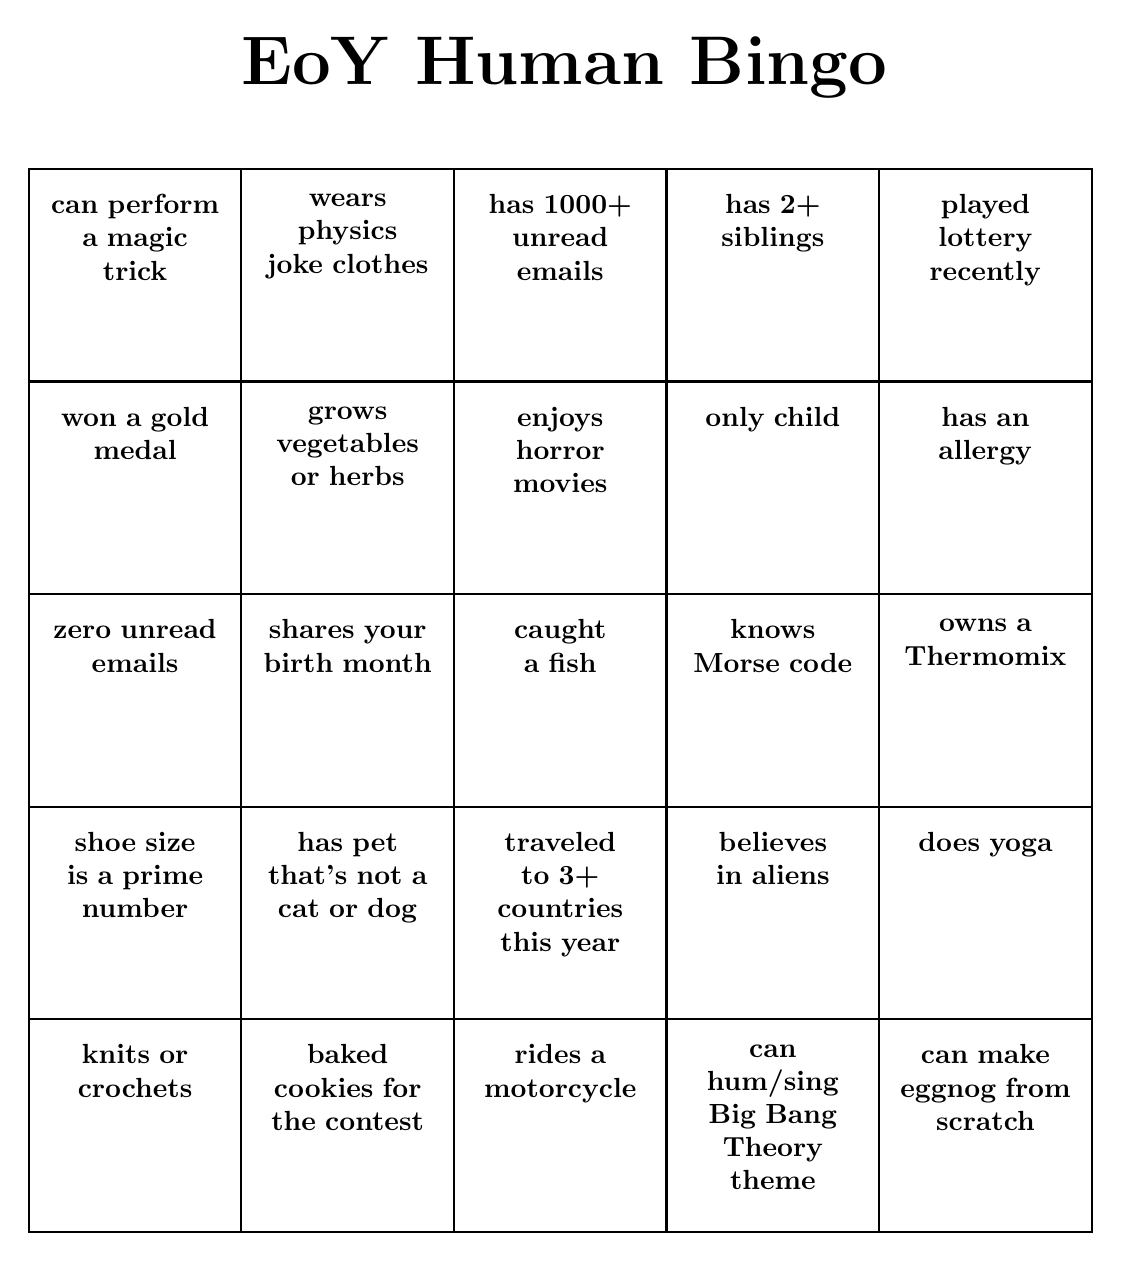
\begin{tikzpicture}
% Set the grid dimensions
\def\cellsize{2.7cm} % Each cell will be 2x2 cm

% Draw the grid and insert the numbers
\draw[thick] (0.0, 0.0) rectangle +(2.7, 2.7);
\node[anchor=north, align=center, text width=2.2cm] at (1.35, 2.5) {\textbf{can perform a magic trick}};
\draw[thick] (2.7, 0.0) rectangle +(2.7, 2.7);
\node[anchor=north, align=center, text width=2.2cm] at (4.050000000000001, 2.5) {\textbf{wears physics joke clothes}};
\draw[thick] (5.4, 0.0) rectangle +(2.7, 2.7);
\node[anchor=north, align=center, text width=2.2cm] at (6.75, 2.5) {\textbf{has 1000+ unread emails}};
\draw[thick] (8.100000000000001, 0.0) rectangle +(2.7, 2.7);
\node[anchor=north, align=center, text width=2.2cm] at (9.450000000000001, 2.5) {\textbf{has 2+ siblings}};
\draw[thick] (10.8, 0.0) rectangle +(2.7, 2.7);
\node[anchor=north, align=center, text width=2.2cm] at (12.15, 2.5) {\textbf{played lottery recently}};
\draw[thick] (0.0, -2.7) rectangle +(2.7, 2.7);
\node[anchor=north, align=center, text width=2.2cm] at (1.35, -0.2) {\textbf{won a gold medal}};
\draw[thick] (2.7, -2.7) rectangle +(2.7, 2.7);
\node[anchor=north, align=center, text width=2.2cm] at (4.050000000000001, -0.2) {\textbf{grows vegetables or herbs}};
\draw[thick] (5.4, -2.7) rectangle +(2.7, 2.7);
\node[anchor=north, align=center, text width=2.2cm] at (6.75, -0.2) {\textbf{enjoys horror movies}};
\draw[thick] (8.100000000000001, -2.7) rectangle +(2.7, 2.7);
\node[anchor=north, align=center, text width=2.2cm] at (9.450000000000001, -0.2) {\textbf{only child}};
\draw[thick] (10.8, -2.7) rectangle +(2.7, 2.7);
\node[anchor=north, align=center, text width=2.2cm] at (12.15, -0.2) {\textbf{has an allergy}};
\draw[thick] (0.0, -5.4) rectangle +(2.7, 2.7);
\node[anchor=north, align=center, text width=2.2cm] at (1.35, -2.9000000000000004) {\textbf{zero unread emails}};
\draw[thick] (2.7, -5.4) rectangle +(2.7, 2.7);
\node[anchor=north, align=center, text width=2.2cm] at (4.050000000000001, -2.9000000000000004) {\textbf{shares your birth month}};
\draw[thick] (5.4, -5.4) rectangle +(2.7, 2.7);
\node[anchor=north, align=center, text width=2.2cm] at (6.75, -2.9000000000000004) {\textbf{caught a fish}};
\draw[thick] (8.100000000000001, -5.4) rectangle +(2.7, 2.7);
\node[anchor=north, align=center, text width=2.2cm] at (9.450000000000001, -2.9000000000000004) {\textbf{knows Morse code}};
\draw[thick] (10.8, -5.4) rectangle +(2.7, 2.7);
\node[anchor=north, align=center, text width=2.2cm] at (12.15, -2.9000000000000004) {\textbf{owns a Thermomix}};
\draw[thick] (0.0, -8.100000000000001) rectangle +(2.7, 2.7);
\node[anchor=north, align=center, text width=2.2cm] at (1.35, -5.600000000000001) {\textbf{shoe size is a prime number}};
\draw[thick] (2.7, -8.100000000000001) rectangle +(2.7, 2.7);
\node[anchor=north, align=center, text width=2.2cm] at (4.050000000000001, -5.600000000000001) {\textbf{has pet that's not a cat or dog}};
\draw[thick] (5.4, -8.100000000000001) rectangle +(2.7, 2.7);
\node[anchor=north, align=center, text width=2.2cm] at (6.75, -5.600000000000001) {\textbf{traveled to 3+ countries this year}};
\draw[thick] (8.100000000000001, -8.100000000000001) rectangle +(2.7, 2.7);
\node[anchor=north, align=center, text width=2.2cm] at (9.450000000000001, -5.600000000000001) {\textbf{believes in aliens}};
\draw[thick] (10.8, -8.100000000000001) rectangle +(2.7, 2.7);
\node[anchor=north, align=center, text width=2.2cm] at (12.15, -5.600000000000001) {\textbf{does yoga}};
\draw[thick] (0.0, -10.8) rectangle +(2.7, 2.7);
\node[anchor=north, align=center, text width=2.2cm] at (1.35, -8.3) {\textbf{knits or crochets}};
\draw[thick] (2.7, -10.8) rectangle +(2.7, 2.7);
\node[anchor=north, align=center, text width=2.2cm] at (4.050000000000001, -8.3) {\textbf{baked cookies for the contest}};
\draw[thick] (5.4, -10.8) rectangle +(2.7, 2.7);
\node[anchor=north, align=center, text width=2.2cm] at (6.75, -8.3) {\textbf{rides a motorcycle}};
\draw[thick] (8.100000000000001, -10.8) rectangle +(2.7, 2.7);
\node[anchor=north, align=center, text width=2.2cm] at (9.450000000000001, -8.3) {\textbf{can hum/sing Big Bang Theory theme}};
\draw[thick] (10.8, -10.8) rectangle +(2.7, 2.7);
\node[anchor=north, align=center, text width=2.2cm] at (12.15, -8.3) {\textbf{can make eggnog from scratch}};
\node[anchor=north, font = \Huge] at (6.8, 4.5){\textbf{EoY Human Bingo}};
\end{tikzpicture}
\end{center}
\newpage\begin{center}
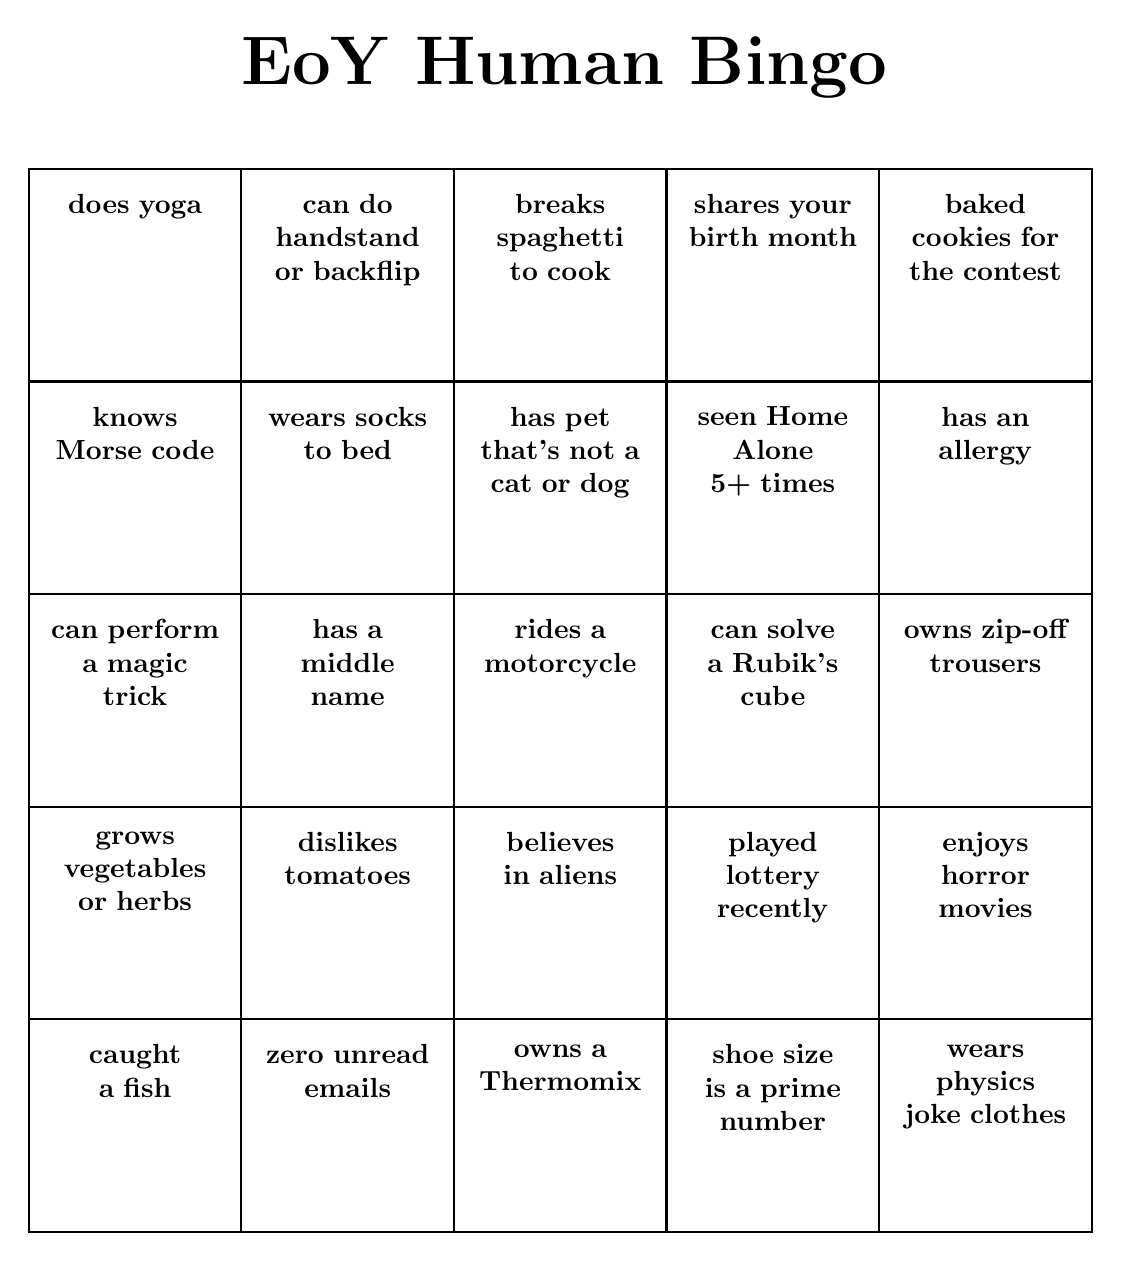
\begin{tikzpicture}
% Set the grid dimensions
\def\cellsize{2.7cm} % Each cell will be 2x2 cm

% Draw the grid and insert the numbers
\draw[thick] (0.0, 0.0) rectangle +(2.7, 2.7);
\node[anchor=north, align=center, text width=2.2cm] at (1.35, 2.5) {\textbf{does yoga}};
\draw[thick] (2.7, 0.0) rectangle +(2.7, 2.7);
\node[anchor=north, align=center, text width=2.2cm] at (4.050000000000001, 2.5) {\textbf{can do handstand or backflip}};
\draw[thick] (5.4, 0.0) rectangle +(2.7, 2.7);
\node[anchor=north, align=center, text width=2.2cm] at (6.75, 2.5) {\textbf{breaks spaghetti to cook}};
\draw[thick] (8.100000000000001, 0.0) rectangle +(2.7, 2.7);
\node[anchor=north, align=center, text width=2.2cm] at (9.450000000000001, 2.5) {\textbf{shares your birth month}};
\draw[thick] (10.8, 0.0) rectangle +(2.7, 2.7);
\node[anchor=north, align=center, text width=2.2cm] at (12.15, 2.5) {\textbf{baked cookies for the contest}};
\draw[thick] (0.0, -2.7) rectangle +(2.7, 2.7);
\node[anchor=north, align=center, text width=2.2cm] at (1.35, -0.2) {\textbf{knows Morse code}};
\draw[thick] (2.7, -2.7) rectangle +(2.7, 2.7);
\node[anchor=north, align=center, text width=2.2cm] at (4.050000000000001, -0.2) {\textbf{wears socks to bed}};
\draw[thick] (5.4, -2.7) rectangle +(2.7, 2.7);
\node[anchor=north, align=center, text width=2.2cm] at (6.75, -0.2) {\textbf{has pet that's not a cat or dog}};
\draw[thick] (8.100000000000001, -2.7) rectangle +(2.7, 2.7);
\node[anchor=north, align=center, text width=2.2cm] at (9.450000000000001, -0.2) {\textbf{seen Home Alone 5+ times}};
\draw[thick] (10.8, -2.7) rectangle +(2.7, 2.7);
\node[anchor=north, align=center, text width=2.2cm] at (12.15, -0.2) {\textbf{has an allergy}};
\draw[thick] (0.0, -5.4) rectangle +(2.7, 2.7);
\node[anchor=north, align=center, text width=2.2cm] at (1.35, -2.9000000000000004) {\textbf{can perform a magic trick}};
\draw[thick] (2.7, -5.4) rectangle +(2.7, 2.7);
\node[anchor=north, align=center, text width=2.2cm] at (4.050000000000001, -2.9000000000000004) {\textbf{has a middle name}};
\draw[thick] (5.4, -5.4) rectangle +(2.7, 2.7);
\node[anchor=north, align=center, text width=2.2cm] at (6.75, -2.9000000000000004) {\textbf{rides a motorcycle}};
\draw[thick] (8.100000000000001, -5.4) rectangle +(2.7, 2.7);
\node[anchor=north, align=center, text width=2.2cm] at (9.450000000000001, -2.9000000000000004) {\textbf{can solve a Rubik's cube}};
\draw[thick] (10.8, -5.4) rectangle +(2.7, 2.7);
\node[anchor=north, align=center, text width=2.2cm] at (12.15, -2.9000000000000004) {\textbf{owns zip-off trousers}};
\draw[thick] (0.0, -8.100000000000001) rectangle +(2.7, 2.7);
\node[anchor=north, align=center, text width=2.2cm] at (1.35, -5.600000000000001) {\textbf{grows vegetables or herbs}};
\draw[thick] (2.7, -8.100000000000001) rectangle +(2.7, 2.7);
\node[anchor=north, align=center, text width=2.2cm] at (4.050000000000001, -5.600000000000001) {\textbf{dislikes tomatoes}};
\draw[thick] (5.4, -8.100000000000001) rectangle +(2.7, 2.7);
\node[anchor=north, align=center, text width=2.2cm] at (6.75, -5.600000000000001) {\textbf{believes in aliens}};
\draw[thick] (8.100000000000001, -8.100000000000001) rectangle +(2.7, 2.7);
\node[anchor=north, align=center, text width=2.2cm] at (9.450000000000001, -5.600000000000001) {\textbf{played lottery recently}};
\draw[thick] (10.8, -8.100000000000001) rectangle +(2.7, 2.7);
\node[anchor=north, align=center, text width=2.2cm] at (12.15, -5.600000000000001) {\textbf{enjoys horror movies}};
\draw[thick] (0.0, -10.8) rectangle +(2.7, 2.7);
\node[anchor=north, align=center, text width=2.2cm] at (1.35, -8.3) {\textbf{caught a fish}};
\draw[thick] (2.7, -10.8) rectangle +(2.7, 2.7);
\node[anchor=north, align=center, text width=2.2cm] at (4.050000000000001, -8.3) {\textbf{zero unread emails}};
\draw[thick] (5.4, -10.8) rectangle +(2.7, 2.7);
\node[anchor=north, align=center, text width=2.2cm] at (6.75, -8.3) {\textbf{owns a Thermomix}};
\draw[thick] (8.100000000000001, -10.8) rectangle +(2.7, 2.7);
\node[anchor=north, align=center, text width=2.2cm] at (9.450000000000001, -8.3) {\textbf{shoe size is a prime number}};
\draw[thick] (10.8, -10.8) rectangle +(2.7, 2.7);
\node[anchor=north, align=center, text width=2.2cm] at (12.15, -8.3) {\textbf{wears physics joke clothes}};
\node[anchor=north, font = \Huge] at (6.8, 4.5){\textbf{EoY Human Bingo}};
\end{tikzpicture}
\end{center}
\newpage\begin{center}
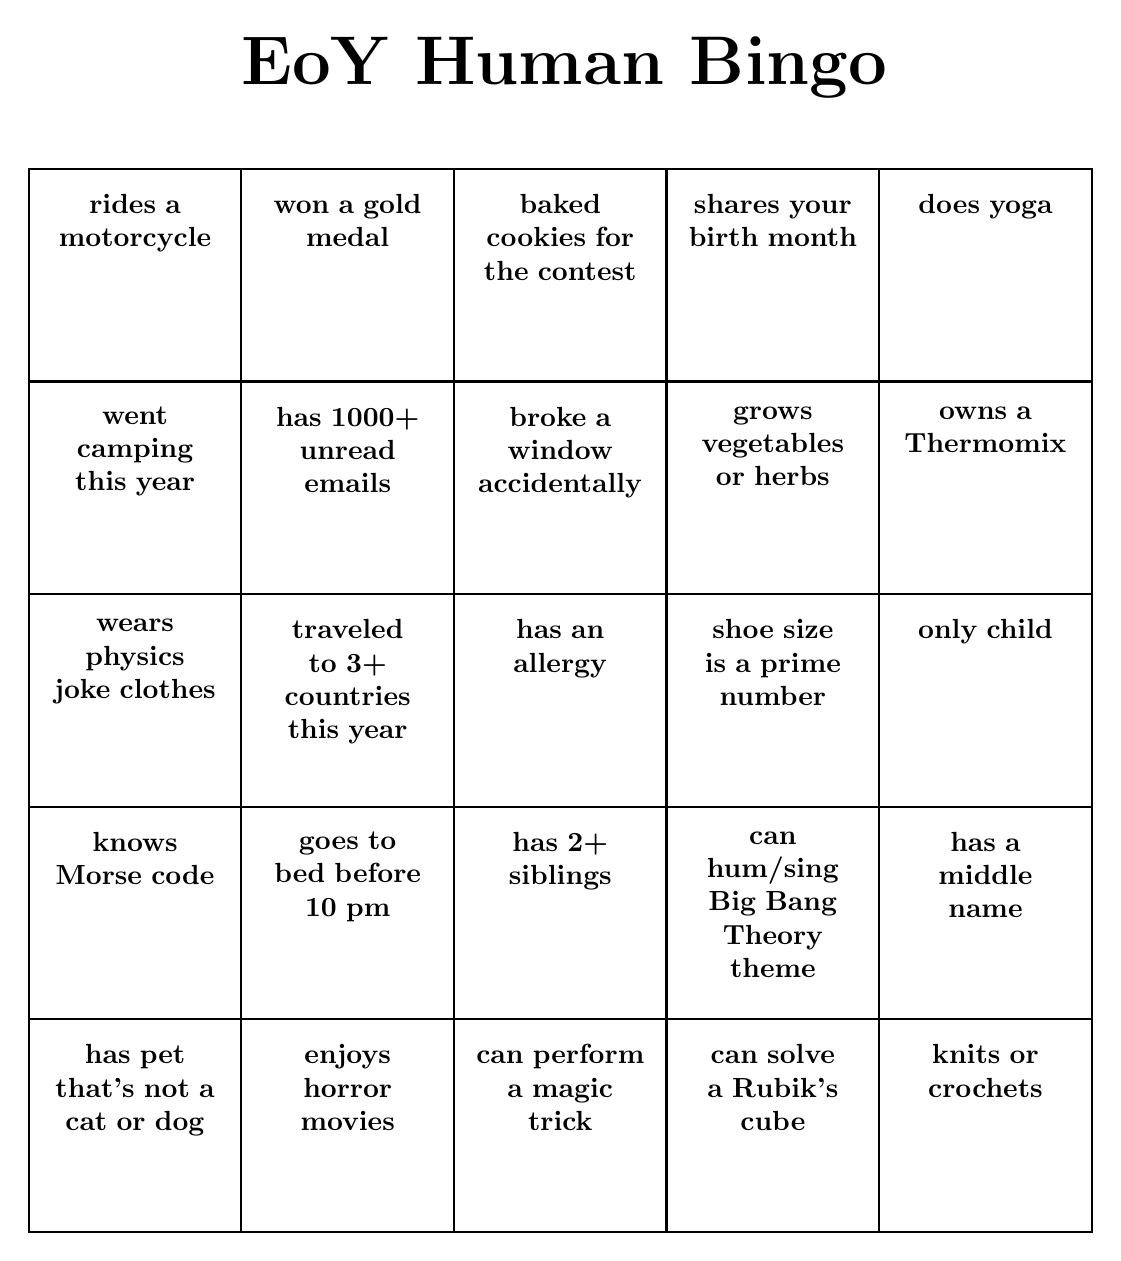
\begin{tikzpicture}
% Set the grid dimensions
\def\cellsize{2.7cm} % Each cell will be 2x2 cm

% Draw the grid and insert the numbers
\draw[thick] (0.0, 0.0) rectangle +(2.7, 2.7);
\node[anchor=north, align=center, text width=2.2cm] at (1.35, 2.5) {\textbf{rides a motorcycle}};
\draw[thick] (2.7, 0.0) rectangle +(2.7, 2.7);
\node[anchor=north, align=center, text width=2.2cm] at (4.050000000000001, 2.5) {\textbf{won a gold medal}};
\draw[thick] (5.4, 0.0) rectangle +(2.7, 2.7);
\node[anchor=north, align=center, text width=2.2cm] at (6.75, 2.5) {\textbf{baked cookies for the contest}};
\draw[thick] (8.100000000000001, 0.0) rectangle +(2.7, 2.7);
\node[anchor=north, align=center, text width=2.2cm] at (9.450000000000001, 2.5) {\textbf{shares your birth month}};
\draw[thick] (10.8, 0.0) rectangle +(2.7, 2.7);
\node[anchor=north, align=center, text width=2.2cm] at (12.15, 2.5) {\textbf{does yoga}};
\draw[thick] (0.0, -2.7) rectangle +(2.7, 2.7);
\node[anchor=north, align=center, text width=2.2cm] at (1.35, -0.2) {\textbf{went camping this year}};
\draw[thick] (2.7, -2.7) rectangle +(2.7, 2.7);
\node[anchor=north, align=center, text width=2.2cm] at (4.050000000000001, -0.2) {\textbf{has 1000+ unread emails}};
\draw[thick] (5.4, -2.7) rectangle +(2.7, 2.7);
\node[anchor=north, align=center, text width=2.2cm] at (6.75, -0.2) {\textbf{broke a window accidentally}};
\draw[thick] (8.100000000000001, -2.7) rectangle +(2.7, 2.7);
\node[anchor=north, align=center, text width=2.2cm] at (9.450000000000001, -0.2) {\textbf{grows vegetables or herbs}};
\draw[thick] (10.8, -2.7) rectangle +(2.7, 2.7);
\node[anchor=north, align=center, text width=2.2cm] at (12.15, -0.2) {\textbf{owns a Thermomix}};
\draw[thick] (0.0, -5.4) rectangle +(2.7, 2.7);
\node[anchor=north, align=center, text width=2.2cm] at (1.35, -2.9000000000000004) {\textbf{wears physics joke clothes}};
\draw[thick] (2.7, -5.4) rectangle +(2.7, 2.7);
\node[anchor=north, align=center, text width=2.2cm] at (4.050000000000001, -2.9000000000000004) {\textbf{traveled to 3+ countries this year}};
\draw[thick] (5.4, -5.4) rectangle +(2.7, 2.7);
\node[anchor=north, align=center, text width=2.2cm] at (6.75, -2.9000000000000004) {\textbf{has an allergy}};
\draw[thick] (8.100000000000001, -5.4) rectangle +(2.7, 2.7);
\node[anchor=north, align=center, text width=2.2cm] at (9.450000000000001, -2.9000000000000004) {\textbf{shoe size is a prime number}};
\draw[thick] (10.8, -5.4) rectangle +(2.7, 2.7);
\node[anchor=north, align=center, text width=2.2cm] at (12.15, -2.9000000000000004) {\textbf{only child}};
\draw[thick] (0.0, -8.100000000000001) rectangle +(2.7, 2.7);
\node[anchor=north, align=center, text width=2.2cm] at (1.35, -5.600000000000001) {\textbf{knows Morse code}};
\draw[thick] (2.7, -8.100000000000001) rectangle +(2.7, 2.7);
\node[anchor=north, align=center, text width=2.2cm] at (4.050000000000001, -5.600000000000001) {\textbf{goes to bed before 10 pm}};
\draw[thick] (5.4, -8.100000000000001) rectangle +(2.7, 2.7);
\node[anchor=north, align=center, text width=2.2cm] at (6.75, -5.600000000000001) {\textbf{has 2+ siblings}};
\draw[thick] (8.100000000000001, -8.100000000000001) rectangle +(2.7, 2.7);
\node[anchor=north, align=center, text width=2.2cm] at (9.450000000000001, -5.600000000000001) {\textbf{can hum/sing Big Bang Theory theme}};
\draw[thick] (10.8, -8.100000000000001) rectangle +(2.7, 2.7);
\node[anchor=north, align=center, text width=2.2cm] at (12.15, -5.600000000000001) {\textbf{has a middle name}};
\draw[thick] (0.0, -10.8) rectangle +(2.7, 2.7);
\node[anchor=north, align=center, text width=2.2cm] at (1.35, -8.3) {\textbf{has pet that's not a cat or dog}};
\draw[thick] (2.7, -10.8) rectangle +(2.7, 2.7);
\node[anchor=north, align=center, text width=2.2cm] at (4.050000000000001, -8.3) {\textbf{enjoys horror movies}};
\draw[thick] (5.4, -10.8) rectangle +(2.7, 2.7);
\node[anchor=north, align=center, text width=2.2cm] at (6.75, -8.3) {\textbf{can perform a magic trick}};
\draw[thick] (8.100000000000001, -10.8) rectangle +(2.7, 2.7);
\node[anchor=north, align=center, text width=2.2cm] at (9.450000000000001, -8.3) {\textbf{can solve a Rubik's cube}};
\draw[thick] (10.8, -10.8) rectangle +(2.7, 2.7);
\node[anchor=north, align=center, text width=2.2cm] at (12.15, -8.3) {\textbf{knits or crochets}};
\node[anchor=north, font = \Huge] at (6.8, 4.5){\textbf{EoY Human Bingo}};
\end{tikzpicture}
\end{center}
\newpage\begin{center}
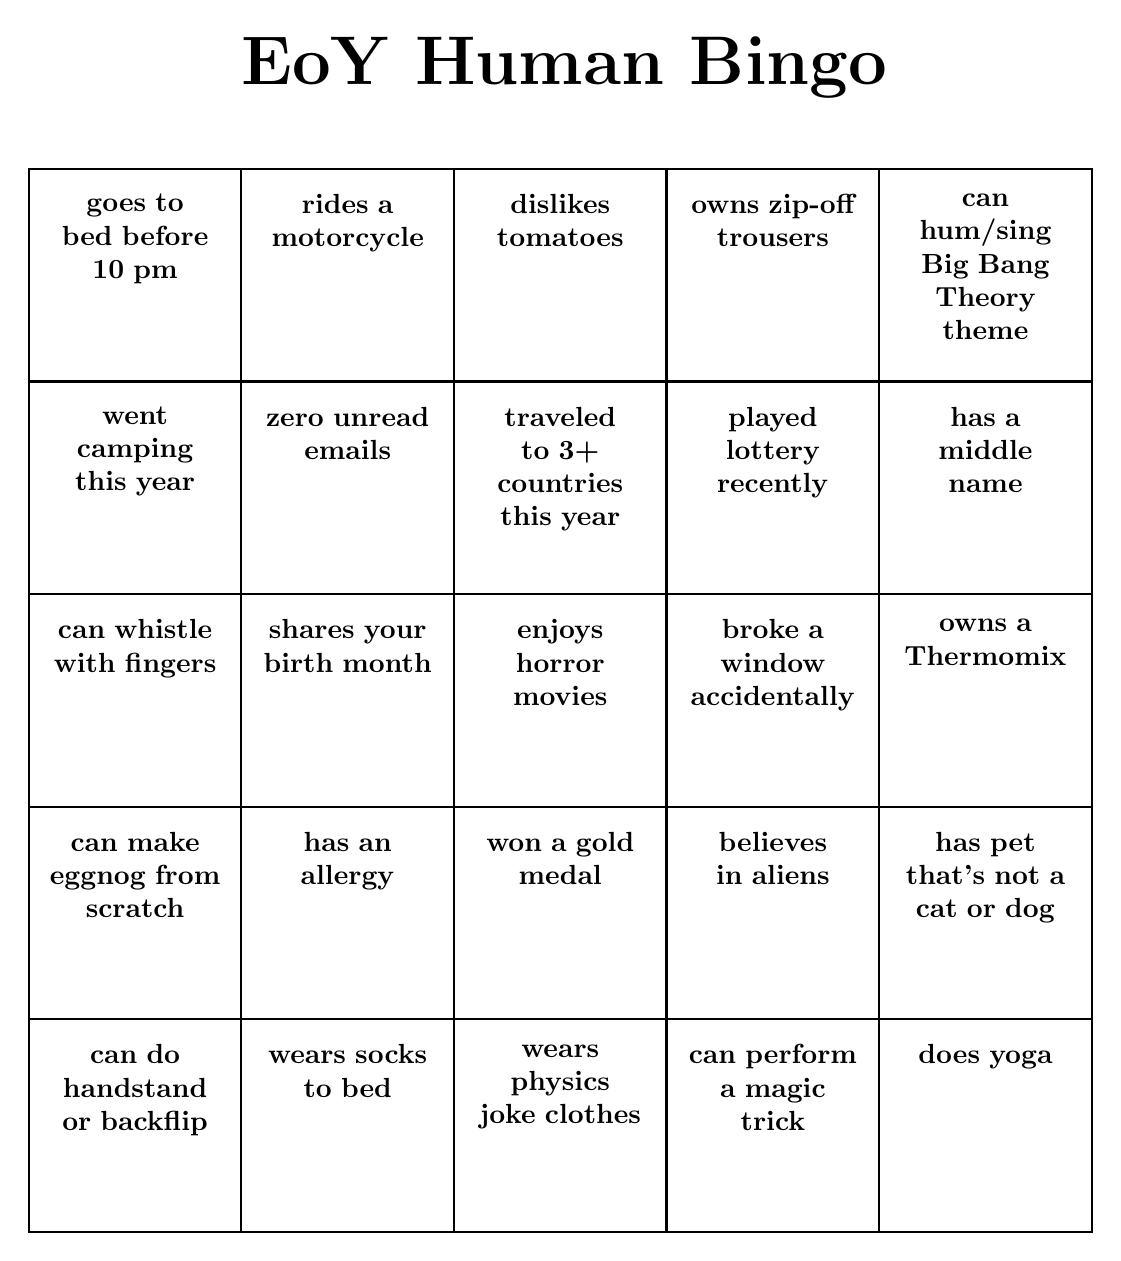
\begin{tikzpicture}
% Set the grid dimensions
\def\cellsize{2.7cm} % Each cell will be 2x2 cm

% Draw the grid and insert the numbers
\draw[thick] (0.0, 0.0) rectangle +(2.7, 2.7);
\node[anchor=north, align=center, text width=2.2cm] at (1.35, 2.5) {\textbf{goes to bed before 10 pm}};
\draw[thick] (2.7, 0.0) rectangle +(2.7, 2.7);
\node[anchor=north, align=center, text width=2.2cm] at (4.050000000000001, 2.5) {\textbf{rides a motorcycle}};
\draw[thick] (5.4, 0.0) rectangle +(2.7, 2.7);
\node[anchor=north, align=center, text width=2.2cm] at (6.75, 2.5) {\textbf{dislikes tomatoes}};
\draw[thick] (8.100000000000001, 0.0) rectangle +(2.7, 2.7);
\node[anchor=north, align=center, text width=2.2cm] at (9.450000000000001, 2.5) {\textbf{owns zip-off trousers}};
\draw[thick] (10.8, 0.0) rectangle +(2.7, 2.7);
\node[anchor=north, align=center, text width=2.2cm] at (12.15, 2.5) {\textbf{can hum/sing Big Bang Theory theme}};
\draw[thick] (0.0, -2.7) rectangle +(2.7, 2.7);
\node[anchor=north, align=center, text width=2.2cm] at (1.35, -0.2) {\textbf{went camping this year}};
\draw[thick] (2.7, -2.7) rectangle +(2.7, 2.7);
\node[anchor=north, align=center, text width=2.2cm] at (4.050000000000001, -0.2) {\textbf{zero unread emails}};
\draw[thick] (5.4, -2.7) rectangle +(2.7, 2.7);
\node[anchor=north, align=center, text width=2.2cm] at (6.75, -0.2) {\textbf{traveled to 3+ countries this year}};
\draw[thick] (8.100000000000001, -2.7) rectangle +(2.7, 2.7);
\node[anchor=north, align=center, text width=2.2cm] at (9.450000000000001, -0.2) {\textbf{played lottery recently}};
\draw[thick] (10.8, -2.7) rectangle +(2.7, 2.7);
\node[anchor=north, align=center, text width=2.2cm] at (12.15, -0.2) {\textbf{has a middle name}};
\draw[thick] (0.0, -5.4) rectangle +(2.7, 2.7);
\node[anchor=north, align=center, text width=2.2cm] at (1.35, -2.9000000000000004) {\textbf{can whistle with fingers}};
\draw[thick] (2.7, -5.4) rectangle +(2.7, 2.7);
\node[anchor=north, align=center, text width=2.2cm] at (4.050000000000001, -2.9000000000000004) {\textbf{shares your birth month}};
\draw[thick] (5.4, -5.4) rectangle +(2.7, 2.7);
\node[anchor=north, align=center, text width=2.2cm] at (6.75, -2.9000000000000004) {\textbf{enjoys horror movies}};
\draw[thick] (8.100000000000001, -5.4) rectangle +(2.7, 2.7);
\node[anchor=north, align=center, text width=2.2cm] at (9.450000000000001, -2.9000000000000004) {\textbf{broke a window accidentally}};
\draw[thick] (10.8, -5.4) rectangle +(2.7, 2.7);
\node[anchor=north, align=center, text width=2.2cm] at (12.15, -2.9000000000000004) {\textbf{owns a Thermomix}};
\draw[thick] (0.0, -8.100000000000001) rectangle +(2.7, 2.7);
\node[anchor=north, align=center, text width=2.2cm] at (1.35, -5.600000000000001) {\textbf{can make eggnog from scratch}};
\draw[thick] (2.7, -8.100000000000001) rectangle +(2.7, 2.7);
\node[anchor=north, align=center, text width=2.2cm] at (4.050000000000001, -5.600000000000001) {\textbf{has an allergy}};
\draw[thick] (5.4, -8.100000000000001) rectangle +(2.7, 2.7);
\node[anchor=north, align=center, text width=2.2cm] at (6.75, -5.600000000000001) {\textbf{won a gold medal}};
\draw[thick] (8.100000000000001, -8.100000000000001) rectangle +(2.7, 2.7);
\node[anchor=north, align=center, text width=2.2cm] at (9.450000000000001, -5.600000000000001) {\textbf{believes in aliens}};
\draw[thick] (10.8, -8.100000000000001) rectangle +(2.7, 2.7);
\node[anchor=north, align=center, text width=2.2cm] at (12.15, -5.600000000000001) {\textbf{has pet that's not a cat or dog}};
\draw[thick] (0.0, -10.8) rectangle +(2.7, 2.7);
\node[anchor=north, align=center, text width=2.2cm] at (1.35, -8.3) {\textbf{can do handstand or backflip}};
\draw[thick] (2.7, -10.8) rectangle +(2.7, 2.7);
\node[anchor=north, align=center, text width=2.2cm] at (4.050000000000001, -8.3) {\textbf{wears socks to bed}};
\draw[thick] (5.4, -10.8) rectangle +(2.7, 2.7);
\node[anchor=north, align=center, text width=2.2cm] at (6.75, -8.3) {\textbf{wears physics joke clothes}};
\draw[thick] (8.100000000000001, -10.8) rectangle +(2.7, 2.7);
\node[anchor=north, align=center, text width=2.2cm] at (9.450000000000001, -8.3) {\textbf{can perform a magic trick}};
\draw[thick] (10.8, -10.8) rectangle +(2.7, 2.7);
\node[anchor=north, align=center, text width=2.2cm] at (12.15, -8.3) {\textbf{does yoga}};
\node[anchor=north, font = \Huge] at (6.8, 4.5){\textbf{EoY Human Bingo}};
\end{tikzpicture}
\end{center}
\newpage\begin{center}
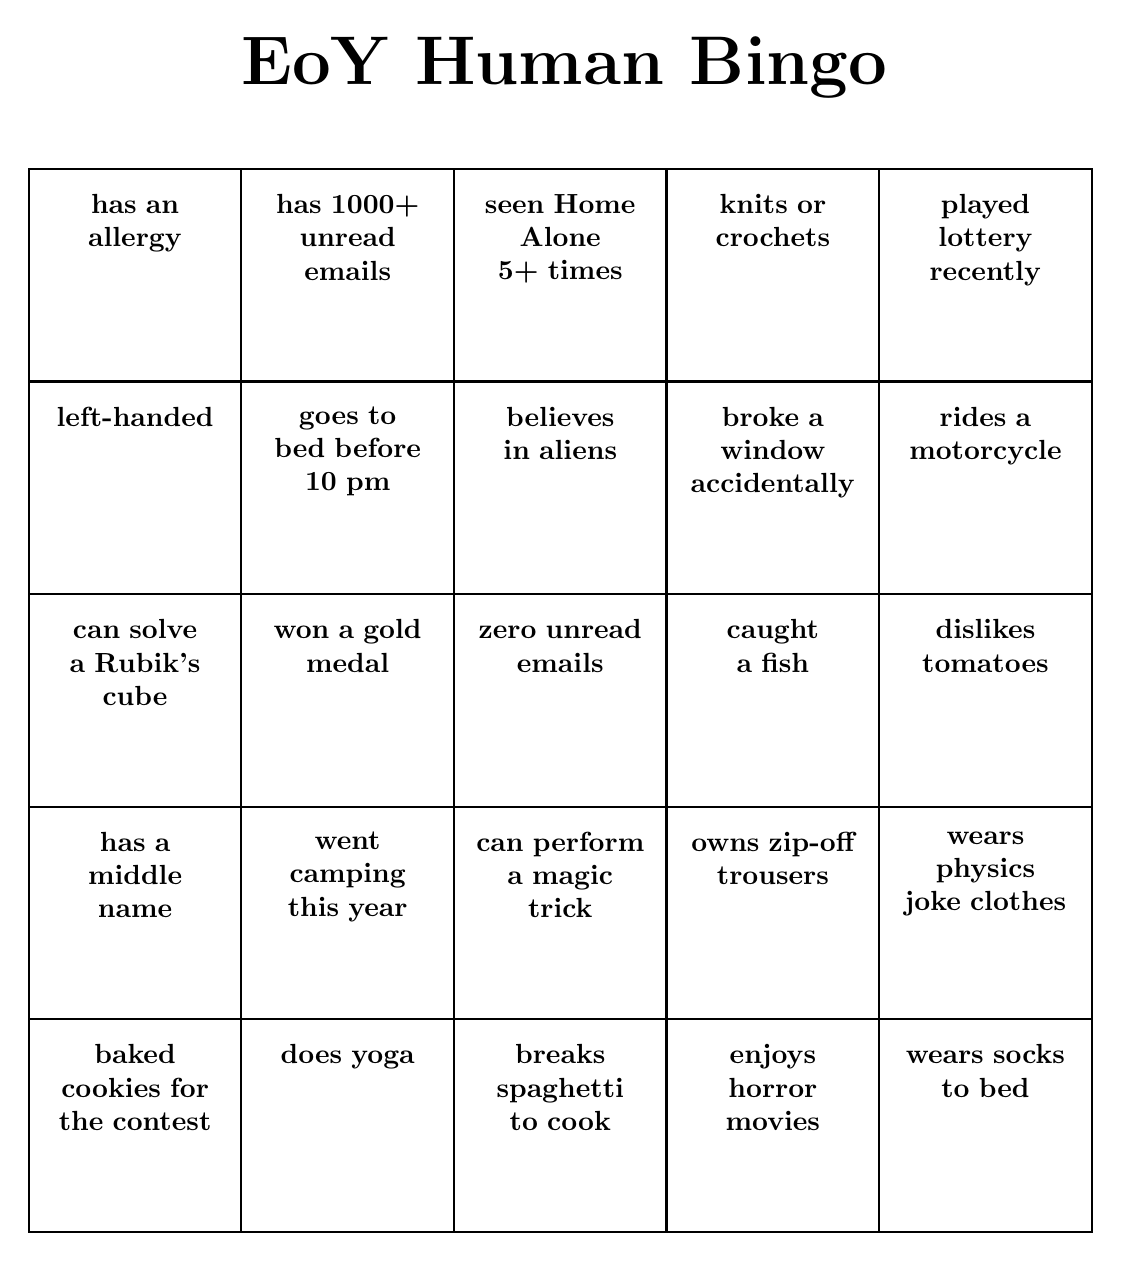
\begin{tikzpicture}
% Set the grid dimensions
\def\cellsize{2.7cm} % Each cell will be 2x2 cm

% Draw the grid and insert the numbers
\draw[thick] (0.0, 0.0) rectangle +(2.7, 2.7);
\node[anchor=north, align=center, text width=2.2cm] at (1.35, 2.5) {\textbf{has an allergy}};
\draw[thick] (2.7, 0.0) rectangle +(2.7, 2.7);
\node[anchor=north, align=center, text width=2.2cm] at (4.050000000000001, 2.5) {\textbf{has 1000+ unread emails}};
\draw[thick] (5.4, 0.0) rectangle +(2.7, 2.7);
\node[anchor=north, align=center, text width=2.2cm] at (6.75, 2.5) {\textbf{seen Home Alone 5+ times}};
\draw[thick] (8.100000000000001, 0.0) rectangle +(2.7, 2.7);
\node[anchor=north, align=center, text width=2.2cm] at (9.450000000000001, 2.5) {\textbf{knits or crochets}};
\draw[thick] (10.8, 0.0) rectangle +(2.7, 2.7);
\node[anchor=north, align=center, text width=2.2cm] at (12.15, 2.5) {\textbf{played lottery recently}};
\draw[thick] (0.0, -2.7) rectangle +(2.7, 2.7);
\node[anchor=north, align=center, text width=2.2cm] at (1.35, -0.2) {\textbf{left-handed}};
\draw[thick] (2.7, -2.7) rectangle +(2.7, 2.7);
\node[anchor=north, align=center, text width=2.2cm] at (4.050000000000001, -0.2) {\textbf{goes to bed before 10 pm}};
\draw[thick] (5.4, -2.7) rectangle +(2.7, 2.7);
\node[anchor=north, align=center, text width=2.2cm] at (6.75, -0.2) {\textbf{believes in aliens}};
\draw[thick] (8.100000000000001, -2.7) rectangle +(2.7, 2.7);
\node[anchor=north, align=center, text width=2.2cm] at (9.450000000000001, -0.2) {\textbf{broke a window accidentally}};
\draw[thick] (10.8, -2.7) rectangle +(2.7, 2.7);
\node[anchor=north, align=center, text width=2.2cm] at (12.15, -0.2) {\textbf{rides a motorcycle}};
\draw[thick] (0.0, -5.4) rectangle +(2.7, 2.7);
\node[anchor=north, align=center, text width=2.2cm] at (1.35, -2.9000000000000004) {\textbf{can solve a Rubik's cube}};
\draw[thick] (2.7, -5.4) rectangle +(2.7, 2.7);
\node[anchor=north, align=center, text width=2.2cm] at (4.050000000000001, -2.9000000000000004) {\textbf{won a gold medal}};
\draw[thick] (5.4, -5.4) rectangle +(2.7, 2.7);
\node[anchor=north, align=center, text width=2.2cm] at (6.75, -2.9000000000000004) {\textbf{zero unread emails}};
\draw[thick] (8.100000000000001, -5.4) rectangle +(2.7, 2.7);
\node[anchor=north, align=center, text width=2.2cm] at (9.450000000000001, -2.9000000000000004) {\textbf{caught a fish}};
\draw[thick] (10.8, -5.4) rectangle +(2.7, 2.7);
\node[anchor=north, align=center, text width=2.2cm] at (12.15, -2.9000000000000004) {\textbf{dislikes tomatoes}};
\draw[thick] (0.0, -8.100000000000001) rectangle +(2.7, 2.7);
\node[anchor=north, align=center, text width=2.2cm] at (1.35, -5.600000000000001) {\textbf{has a middle name}};
\draw[thick] (2.7, -8.100000000000001) rectangle +(2.7, 2.7);
\node[anchor=north, align=center, text width=2.2cm] at (4.050000000000001, -5.600000000000001) {\textbf{went camping this year}};
\draw[thick] (5.4, -8.100000000000001) rectangle +(2.7, 2.7);
\node[anchor=north, align=center, text width=2.2cm] at (6.75, -5.600000000000001) {\textbf{can perform a magic trick}};
\draw[thick] (8.100000000000001, -8.100000000000001) rectangle +(2.7, 2.7);
\node[anchor=north, align=center, text width=2.2cm] at (9.450000000000001, -5.600000000000001) {\textbf{owns zip-off trousers}};
\draw[thick] (10.8, -8.100000000000001) rectangle +(2.7, 2.7);
\node[anchor=north, align=center, text width=2.2cm] at (12.15, -5.600000000000001) {\textbf{wears physics joke clothes}};
\draw[thick] (0.0, -10.8) rectangle +(2.7, 2.7);
\node[anchor=north, align=center, text width=2.2cm] at (1.35, -8.3) {\textbf{baked cookies for the contest}};
\draw[thick] (2.7, -10.8) rectangle +(2.7, 2.7);
\node[anchor=north, align=center, text width=2.2cm] at (4.050000000000001, -8.3) {\textbf{does yoga}};
\draw[thick] (5.4, -10.8) rectangle +(2.7, 2.7);
\node[anchor=north, align=center, text width=2.2cm] at (6.75, -8.3) {\textbf{breaks spaghetti to cook}};
\draw[thick] (8.100000000000001, -10.8) rectangle +(2.7, 2.7);
\node[anchor=north, align=center, text width=2.2cm] at (9.450000000000001, -8.3) {\textbf{enjoys horror movies}};
\draw[thick] (10.8, -10.8) rectangle +(2.7, 2.7);
\node[anchor=north, align=center, text width=2.2cm] at (12.15, -8.3) {\textbf{wears socks to bed}};
\node[anchor=north, font = \Huge] at (6.8, 4.5){\textbf{EoY Human Bingo}};
\end{tikzpicture}
\end{center}
\newpage\begin{center}
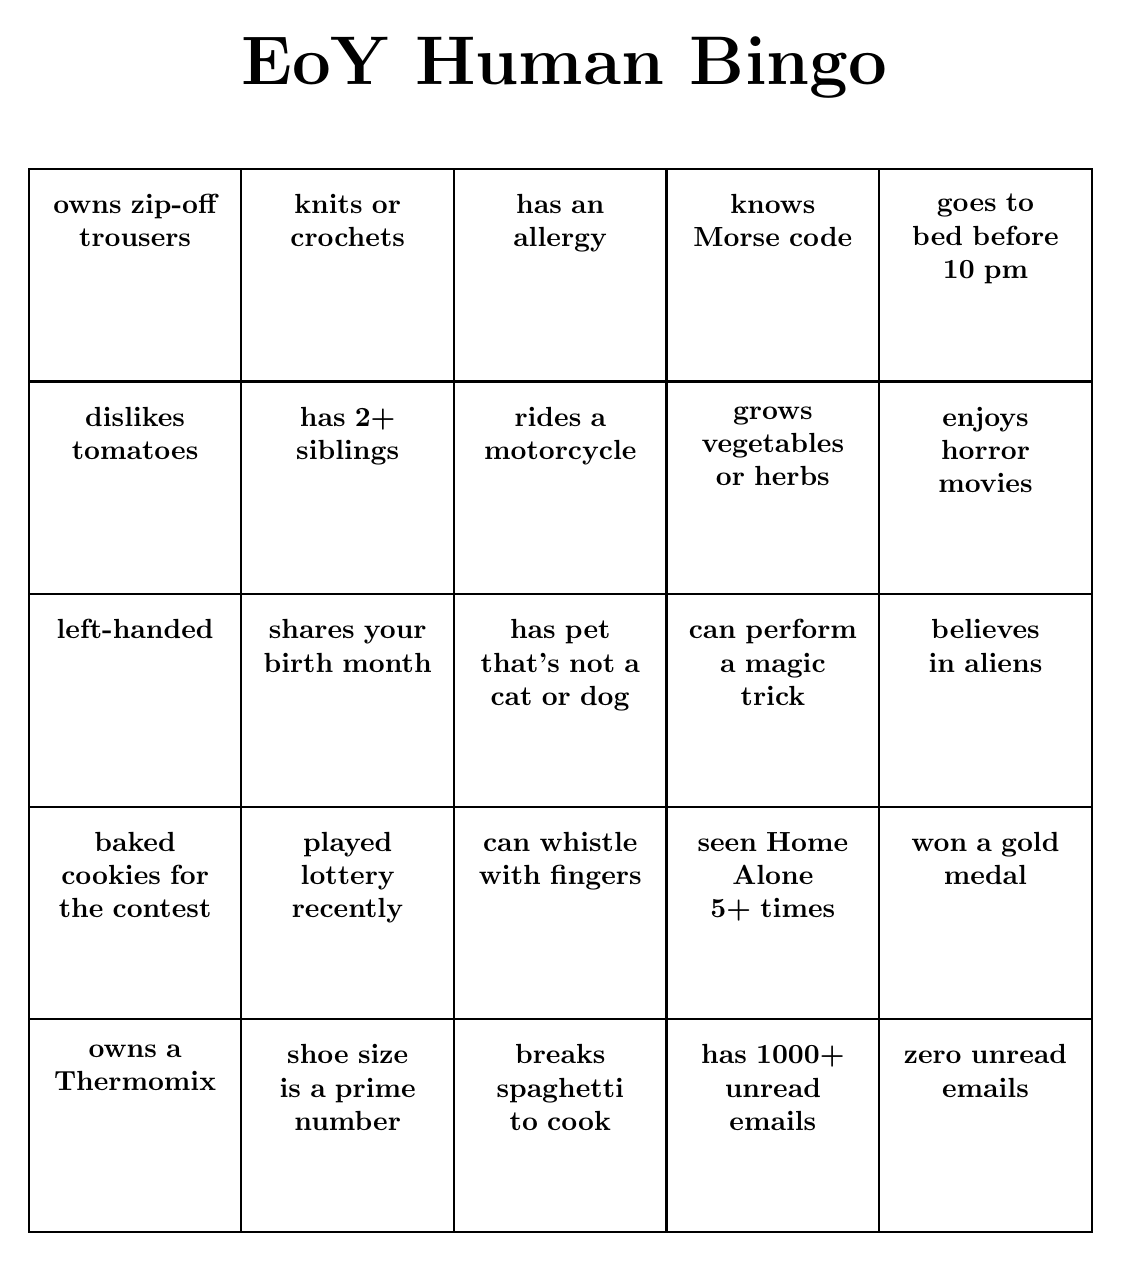
\begin{tikzpicture}
% Set the grid dimensions
\def\cellsize{2.7cm} % Each cell will be 2x2 cm

% Draw the grid and insert the numbers
\draw[thick] (0.0, 0.0) rectangle +(2.7, 2.7);
\node[anchor=north, align=center, text width=2.2cm] at (1.35, 2.5) {\textbf{owns zip-off trousers}};
\draw[thick] (2.7, 0.0) rectangle +(2.7, 2.7);
\node[anchor=north, align=center, text width=2.2cm] at (4.050000000000001, 2.5) {\textbf{knits or crochets}};
\draw[thick] (5.4, 0.0) rectangle +(2.7, 2.7);
\node[anchor=north, align=center, text width=2.2cm] at (6.75, 2.5) {\textbf{has an allergy}};
\draw[thick] (8.100000000000001, 0.0) rectangle +(2.7, 2.7);
\node[anchor=north, align=center, text width=2.2cm] at (9.450000000000001, 2.5) {\textbf{knows Morse code}};
\draw[thick] (10.8, 0.0) rectangle +(2.7, 2.7);
\node[anchor=north, align=center, text width=2.2cm] at (12.15, 2.5) {\textbf{goes to bed before 10 pm}};
\draw[thick] (0.0, -2.7) rectangle +(2.7, 2.7);
\node[anchor=north, align=center, text width=2.2cm] at (1.35, -0.2) {\textbf{dislikes tomatoes}};
\draw[thick] (2.7, -2.7) rectangle +(2.7, 2.7);
\node[anchor=north, align=center, text width=2.2cm] at (4.050000000000001, -0.2) {\textbf{has 2+ siblings}};
\draw[thick] (5.4, -2.7) rectangle +(2.7, 2.7);
\node[anchor=north, align=center, text width=2.2cm] at (6.75, -0.2) {\textbf{rides a motorcycle}};
\draw[thick] (8.100000000000001, -2.7) rectangle +(2.7, 2.7);
\node[anchor=north, align=center, text width=2.2cm] at (9.450000000000001, -0.2) {\textbf{grows vegetables or herbs}};
\draw[thick] (10.8, -2.7) rectangle +(2.7, 2.7);
\node[anchor=north, align=center, text width=2.2cm] at (12.15, -0.2) {\textbf{enjoys horror movies}};
\draw[thick] (0.0, -5.4) rectangle +(2.7, 2.7);
\node[anchor=north, align=center, text width=2.2cm] at (1.35, -2.9000000000000004) {\textbf{left-handed}};
\draw[thick] (2.7, -5.4) rectangle +(2.7, 2.7);
\node[anchor=north, align=center, text width=2.2cm] at (4.050000000000001, -2.9000000000000004) {\textbf{shares your birth month}};
\draw[thick] (5.4, -5.4) rectangle +(2.7, 2.7);
\node[anchor=north, align=center, text width=2.2cm] at (6.75, -2.9000000000000004) {\textbf{has pet that's not a cat or dog}};
\draw[thick] (8.100000000000001, -5.4) rectangle +(2.7, 2.7);
\node[anchor=north, align=center, text width=2.2cm] at (9.450000000000001, -2.9000000000000004) {\textbf{can perform a magic trick}};
\draw[thick] (10.8, -5.4) rectangle +(2.7, 2.7);
\node[anchor=north, align=center, text width=2.2cm] at (12.15, -2.9000000000000004) {\textbf{believes in aliens}};
\draw[thick] (0.0, -8.100000000000001) rectangle +(2.7, 2.7);
\node[anchor=north, align=center, text width=2.2cm] at (1.35, -5.600000000000001) {\textbf{baked cookies for the contest}};
\draw[thick] (2.7, -8.100000000000001) rectangle +(2.7, 2.7);
\node[anchor=north, align=center, text width=2.2cm] at (4.050000000000001, -5.600000000000001) {\textbf{played lottery recently}};
\draw[thick] (5.4, -8.100000000000001) rectangle +(2.7, 2.7);
\node[anchor=north, align=center, text width=2.2cm] at (6.75, -5.600000000000001) {\textbf{can whistle with fingers}};
\draw[thick] (8.100000000000001, -8.100000000000001) rectangle +(2.7, 2.7);
\node[anchor=north, align=center, text width=2.2cm] at (9.450000000000001, -5.600000000000001) {\textbf{seen Home Alone 5+ times}};
\draw[thick] (10.8, -8.100000000000001) rectangle +(2.7, 2.7);
\node[anchor=north, align=center, text width=2.2cm] at (12.15, -5.600000000000001) {\textbf{won a gold medal}};
\draw[thick] (0.0, -10.8) rectangle +(2.7, 2.7);
\node[anchor=north, align=center, text width=2.2cm] at (1.35, -8.3) {\textbf{owns a Thermomix}};
\draw[thick] (2.7, -10.8) rectangle +(2.7, 2.7);
\node[anchor=north, align=center, text width=2.2cm] at (4.050000000000001, -8.3) {\textbf{shoe size is a prime number}};
\draw[thick] (5.4, -10.8) rectangle +(2.7, 2.7);
\node[anchor=north, align=center, text width=2.2cm] at (6.75, -8.3) {\textbf{breaks spaghetti to cook}};
\draw[thick] (8.100000000000001, -10.8) rectangle +(2.7, 2.7);
\node[anchor=north, align=center, text width=2.2cm] at (9.450000000000001, -8.3) {\textbf{has 1000+ unread emails}};
\draw[thick] (10.8, -10.8) rectangle +(2.7, 2.7);
\node[anchor=north, align=center, text width=2.2cm] at (12.15, -8.3) {\textbf{zero unread emails}};
\node[anchor=north, font = \Huge] at (6.8, 4.5){\textbf{EoY Human Bingo}};
\end{tikzpicture}
\end{center}
\newpage\begin{center}
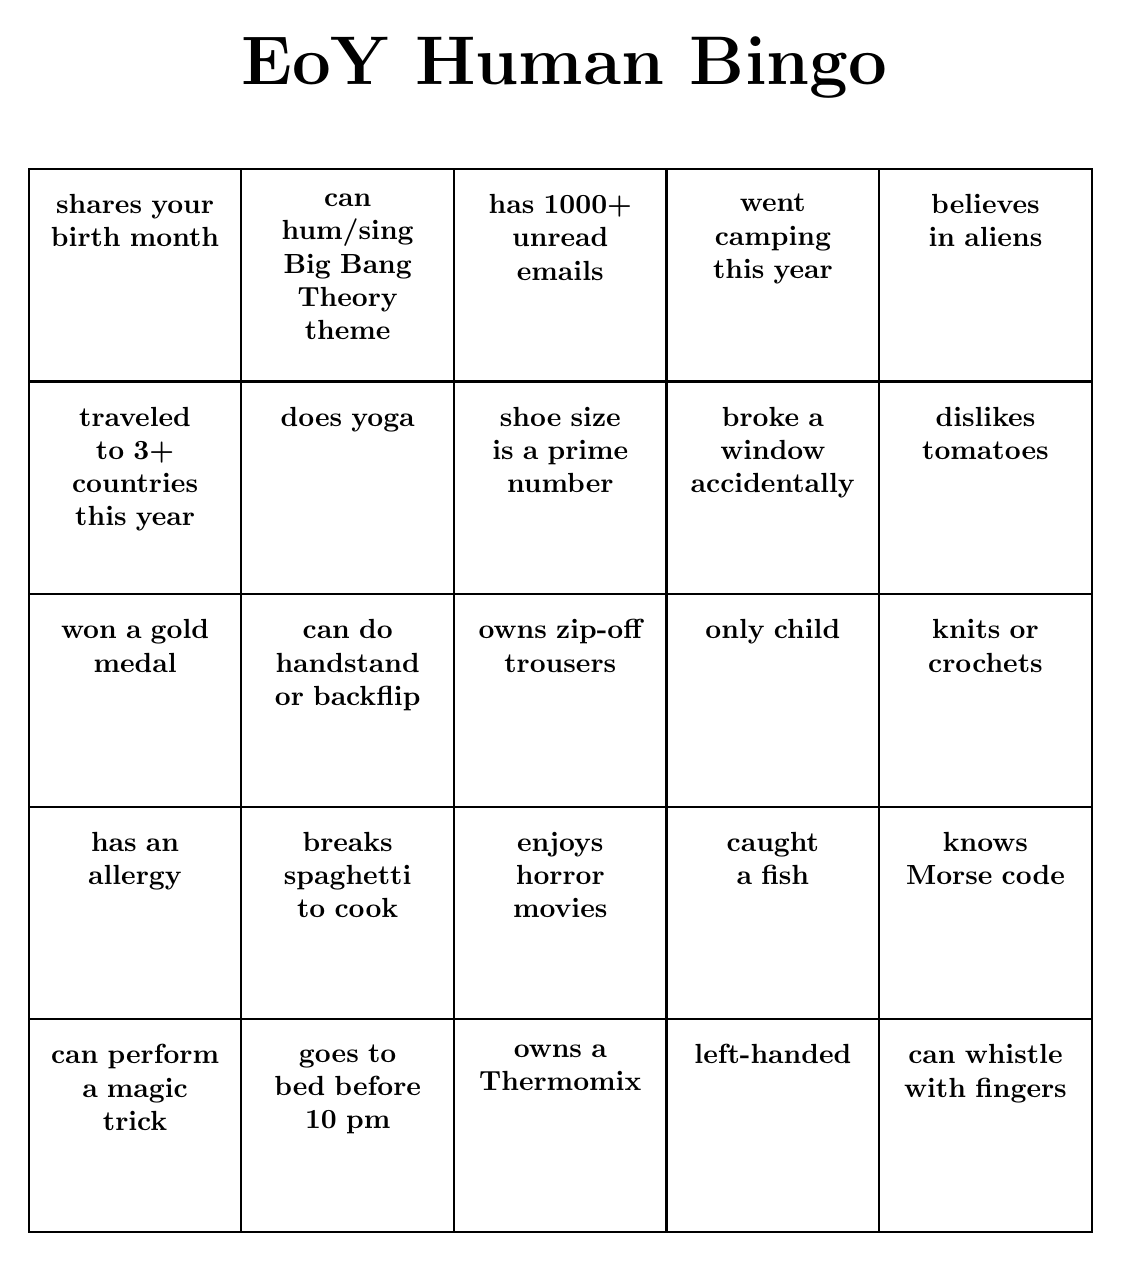
\begin{tikzpicture}
% Set the grid dimensions
\def\cellsize{2.7cm} % Each cell will be 2x2 cm

% Draw the grid and insert the numbers
\draw[thick] (0.0, 0.0) rectangle +(2.7, 2.7);
\node[anchor=north, align=center, text width=2.2cm] at (1.35, 2.5) {\textbf{shares your birth month}};
\draw[thick] (2.7, 0.0) rectangle +(2.7, 2.7);
\node[anchor=north, align=center, text width=2.2cm] at (4.050000000000001, 2.5) {\textbf{can hum/sing Big Bang Theory theme}};
\draw[thick] (5.4, 0.0) rectangle +(2.7, 2.7);
\node[anchor=north, align=center, text width=2.2cm] at (6.75, 2.5) {\textbf{has 1000+ unread emails}};
\draw[thick] (8.100000000000001, 0.0) rectangle +(2.7, 2.7);
\node[anchor=north, align=center, text width=2.2cm] at (9.450000000000001, 2.5) {\textbf{went camping this year}};
\draw[thick] (10.8, 0.0) rectangle +(2.7, 2.7);
\node[anchor=north, align=center, text width=2.2cm] at (12.15, 2.5) {\textbf{believes in aliens}};
\draw[thick] (0.0, -2.7) rectangle +(2.7, 2.7);
\node[anchor=north, align=center, text width=2.2cm] at (1.35, -0.2) {\textbf{traveled to 3+ countries this year}};
\draw[thick] (2.7, -2.7) rectangle +(2.7, 2.7);
\node[anchor=north, align=center, text width=2.2cm] at (4.050000000000001, -0.2) {\textbf{does yoga}};
\draw[thick] (5.4, -2.7) rectangle +(2.7, 2.7);
\node[anchor=north, align=center, text width=2.2cm] at (6.75, -0.2) {\textbf{shoe size is a prime number}};
\draw[thick] (8.100000000000001, -2.7) rectangle +(2.7, 2.7);
\node[anchor=north, align=center, text width=2.2cm] at (9.450000000000001, -0.2) {\textbf{broke a window accidentally}};
\draw[thick] (10.8, -2.7) rectangle +(2.7, 2.7);
\node[anchor=north, align=center, text width=2.2cm] at (12.15, -0.2) {\textbf{dislikes tomatoes}};
\draw[thick] (0.0, -5.4) rectangle +(2.7, 2.7);
\node[anchor=north, align=center, text width=2.2cm] at (1.35, -2.9000000000000004) {\textbf{won a gold medal}};
\draw[thick] (2.7, -5.4) rectangle +(2.7, 2.7);
\node[anchor=north, align=center, text width=2.2cm] at (4.050000000000001, -2.9000000000000004) {\textbf{can do handstand or backflip}};
\draw[thick] (5.4, -5.4) rectangle +(2.7, 2.7);
\node[anchor=north, align=center, text width=2.2cm] at (6.75, -2.9000000000000004) {\textbf{owns zip-off trousers}};
\draw[thick] (8.100000000000001, -5.4) rectangle +(2.7, 2.7);
\node[anchor=north, align=center, text width=2.2cm] at (9.450000000000001, -2.9000000000000004) {\textbf{only child}};
\draw[thick] (10.8, -5.4) rectangle +(2.7, 2.7);
\node[anchor=north, align=center, text width=2.2cm] at (12.15, -2.9000000000000004) {\textbf{knits or crochets}};
\draw[thick] (0.0, -8.100000000000001) rectangle +(2.7, 2.7);
\node[anchor=north, align=center, text width=2.2cm] at (1.35, -5.600000000000001) {\textbf{has an allergy}};
\draw[thick] (2.7, -8.100000000000001) rectangle +(2.7, 2.7);
\node[anchor=north, align=center, text width=2.2cm] at (4.050000000000001, -5.600000000000001) {\textbf{breaks spaghetti to cook}};
\draw[thick] (5.4, -8.100000000000001) rectangle +(2.7, 2.7);
\node[anchor=north, align=center, text width=2.2cm] at (6.75, -5.600000000000001) {\textbf{enjoys horror movies}};
\draw[thick] (8.100000000000001, -8.100000000000001) rectangle +(2.7, 2.7);
\node[anchor=north, align=center, text width=2.2cm] at (9.450000000000001, -5.600000000000001) {\textbf{caught a fish}};
\draw[thick] (10.8, -8.100000000000001) rectangle +(2.7, 2.7);
\node[anchor=north, align=center, text width=2.2cm] at (12.15, -5.600000000000001) {\textbf{knows Morse code}};
\draw[thick] (0.0, -10.8) rectangle +(2.7, 2.7);
\node[anchor=north, align=center, text width=2.2cm] at (1.35, -8.3) {\textbf{can perform a magic trick}};
\draw[thick] (2.7, -10.8) rectangle +(2.7, 2.7);
\node[anchor=north, align=center, text width=2.2cm] at (4.050000000000001, -8.3) {\textbf{goes to bed before 10 pm}};
\draw[thick] (5.4, -10.8) rectangle +(2.7, 2.7);
\node[anchor=north, align=center, text width=2.2cm] at (6.75, -8.3) {\textbf{owns a Thermomix}};
\draw[thick] (8.100000000000001, -10.8) rectangle +(2.7, 2.7);
\node[anchor=north, align=center, text width=2.2cm] at (9.450000000000001, -8.3) {\textbf{left-handed}};
\draw[thick] (10.8, -10.8) rectangle +(2.7, 2.7);
\node[anchor=north, align=center, text width=2.2cm] at (12.15, -8.3) {\textbf{can whistle with fingers}};
\node[anchor=north, font = \Huge] at (6.8, 4.5){\textbf{EoY Human Bingo}};
\end{tikzpicture}
\end{center}
\newpage\begin{center}
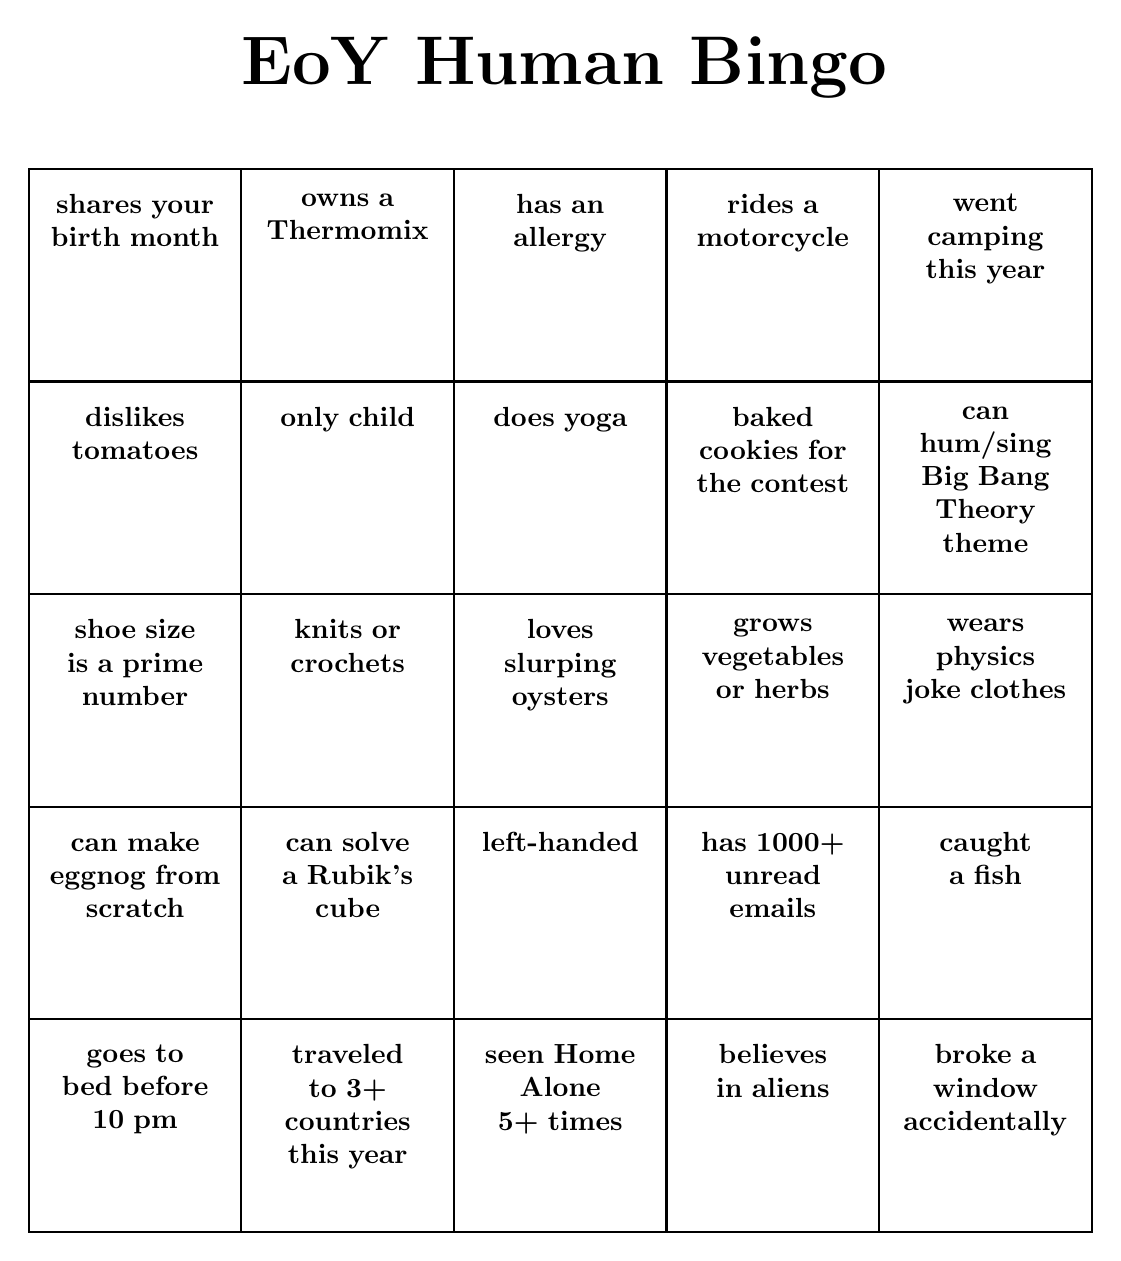
\begin{tikzpicture}
% Set the grid dimensions
\def\cellsize{2.7cm} % Each cell will be 2x2 cm

% Draw the grid and insert the numbers
\draw[thick] (0.0, 0.0) rectangle +(2.7, 2.7);
\node[anchor=north, align=center, text width=2.2cm] at (1.35, 2.5) {\textbf{shares your birth month}};
\draw[thick] (2.7, 0.0) rectangle +(2.7, 2.7);
\node[anchor=north, align=center, text width=2.2cm] at (4.050000000000001, 2.5) {\textbf{owns a Thermomix}};
\draw[thick] (5.4, 0.0) rectangle +(2.7, 2.7);
\node[anchor=north, align=center, text width=2.2cm] at (6.75, 2.5) {\textbf{has an allergy}};
\draw[thick] (8.100000000000001, 0.0) rectangle +(2.7, 2.7);
\node[anchor=north, align=center, text width=2.2cm] at (9.450000000000001, 2.5) {\textbf{rides a motorcycle}};
\draw[thick] (10.8, 0.0) rectangle +(2.7, 2.7);
\node[anchor=north, align=center, text width=2.2cm] at (12.15, 2.5) {\textbf{went camping this year}};
\draw[thick] (0.0, -2.7) rectangle +(2.7, 2.7);
\node[anchor=north, align=center, text width=2.2cm] at (1.35, -0.2) {\textbf{dislikes tomatoes}};
\draw[thick] (2.7, -2.7) rectangle +(2.7, 2.7);
\node[anchor=north, align=center, text width=2.2cm] at (4.050000000000001, -0.2) {\textbf{only child}};
\draw[thick] (5.4, -2.7) rectangle +(2.7, 2.7);
\node[anchor=north, align=center, text width=2.2cm] at (6.75, -0.2) {\textbf{does yoga}};
\draw[thick] (8.100000000000001, -2.7) rectangle +(2.7, 2.7);
\node[anchor=north, align=center, text width=2.2cm] at (9.450000000000001, -0.2) {\textbf{baked cookies for the contest}};
\draw[thick] (10.8, -2.7) rectangle +(2.7, 2.7);
\node[anchor=north, align=center, text width=2.2cm] at (12.15, -0.2) {\textbf{can hum/sing Big Bang Theory theme}};
\draw[thick] (0.0, -5.4) rectangle +(2.7, 2.7);
\node[anchor=north, align=center, text width=2.2cm] at (1.35, -2.9000000000000004) {\textbf{shoe size is a prime number}};
\draw[thick] (2.7, -5.4) rectangle +(2.7, 2.7);
\node[anchor=north, align=center, text width=2.2cm] at (4.050000000000001, -2.9000000000000004) {\textbf{knits or crochets}};
\draw[thick] (5.4, -5.4) rectangle +(2.7, 2.7);
\node[anchor=north, align=center, text width=2.2cm] at (6.75, -2.9000000000000004) {\textbf{loves slurping oysters}};
\draw[thick] (8.100000000000001, -5.4) rectangle +(2.7, 2.7);
\node[anchor=north, align=center, text width=2.2cm] at (9.450000000000001, -2.9000000000000004) {\textbf{grows vegetables or herbs}};
\draw[thick] (10.8, -5.4) rectangle +(2.7, 2.7);
\node[anchor=north, align=center, text width=2.2cm] at (12.15, -2.9000000000000004) {\textbf{wears physics joke clothes}};
\draw[thick] (0.0, -8.100000000000001) rectangle +(2.7, 2.7);
\node[anchor=north, align=center, text width=2.2cm] at (1.35, -5.600000000000001) {\textbf{can make eggnog from scratch}};
\draw[thick] (2.7, -8.100000000000001) rectangle +(2.7, 2.7);
\node[anchor=north, align=center, text width=2.2cm] at (4.050000000000001, -5.600000000000001) {\textbf{can solve a Rubik's cube}};
\draw[thick] (5.4, -8.100000000000001) rectangle +(2.7, 2.7);
\node[anchor=north, align=center, text width=2.2cm] at (6.75, -5.600000000000001) {\textbf{left-handed}};
\draw[thick] (8.100000000000001, -8.100000000000001) rectangle +(2.7, 2.7);
\node[anchor=north, align=center, text width=2.2cm] at (9.450000000000001, -5.600000000000001) {\textbf{has 1000+ unread emails}};
\draw[thick] (10.8, -8.100000000000001) rectangle +(2.7, 2.7);
\node[anchor=north, align=center, text width=2.2cm] at (12.15, -5.600000000000001) {\textbf{caught a fish}};
\draw[thick] (0.0, -10.8) rectangle +(2.7, 2.7);
\node[anchor=north, align=center, text width=2.2cm] at (1.35, -8.3) {\textbf{goes to bed before 10 pm}};
\draw[thick] (2.7, -10.8) rectangle +(2.7, 2.7);
\node[anchor=north, align=center, text width=2.2cm] at (4.050000000000001, -8.3) {\textbf{traveled to 3+ countries this year}};
\draw[thick] (5.4, -10.8) rectangle +(2.7, 2.7);
\node[anchor=north, align=center, text width=2.2cm] at (6.75, -8.3) {\textbf{seen Home Alone 5+ times}};
\draw[thick] (8.100000000000001, -10.8) rectangle +(2.7, 2.7);
\node[anchor=north, align=center, text width=2.2cm] at (9.450000000000001, -8.3) {\textbf{believes in aliens}};
\draw[thick] (10.8, -10.8) rectangle +(2.7, 2.7);
\node[anchor=north, align=center, text width=2.2cm] at (12.15, -8.3) {\textbf{broke a window accidentally}};
\node[anchor=north, font = \Huge] at (6.8, 4.5){\textbf{EoY Human Bingo}};
\end{tikzpicture}
\end{center}
\newpage\begin{center}
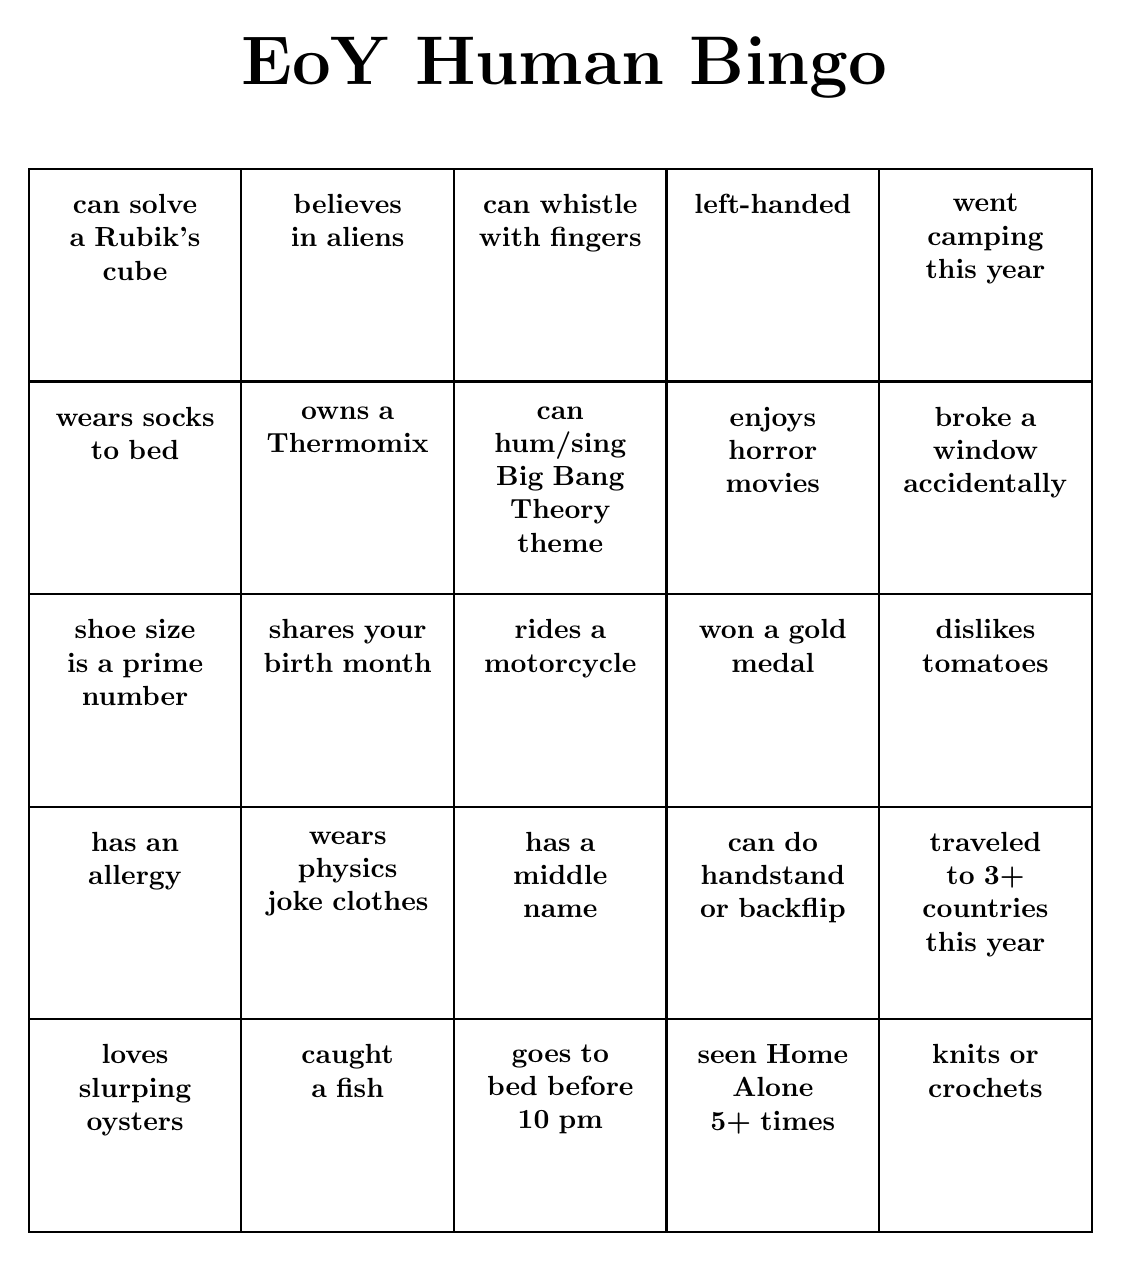
\begin{tikzpicture}
% Set the grid dimensions
\def\cellsize{2.7cm} % Each cell will be 2x2 cm

% Draw the grid and insert the numbers
\draw[thick] (0.0, 0.0) rectangle +(2.7, 2.7);
\node[anchor=north, align=center, text width=2.2cm] at (1.35, 2.5) {\textbf{can solve a Rubik's cube}};
\draw[thick] (2.7, 0.0) rectangle +(2.7, 2.7);
\node[anchor=north, align=center, text width=2.2cm] at (4.050000000000001, 2.5) {\textbf{believes in aliens}};
\draw[thick] (5.4, 0.0) rectangle +(2.7, 2.7);
\node[anchor=north, align=center, text width=2.2cm] at (6.75, 2.5) {\textbf{can whistle with fingers}};
\draw[thick] (8.100000000000001, 0.0) rectangle +(2.7, 2.7);
\node[anchor=north, align=center, text width=2.2cm] at (9.450000000000001, 2.5) {\textbf{left-handed}};
\draw[thick] (10.8, 0.0) rectangle +(2.7, 2.7);
\node[anchor=north, align=center, text width=2.2cm] at (12.15, 2.5) {\textbf{went camping this year}};
\draw[thick] (0.0, -2.7) rectangle +(2.7, 2.7);
\node[anchor=north, align=center, text width=2.2cm] at (1.35, -0.2) {\textbf{wears socks to bed}};
\draw[thick] (2.7, -2.7) rectangle +(2.7, 2.7);
\node[anchor=north, align=center, text width=2.2cm] at (4.050000000000001, -0.2) {\textbf{owns a Thermomix}};
\draw[thick] (5.4, -2.7) rectangle +(2.7, 2.7);
\node[anchor=north, align=center, text width=2.2cm] at (6.75, -0.2) {\textbf{can hum/sing Big Bang Theory theme}};
\draw[thick] (8.100000000000001, -2.7) rectangle +(2.7, 2.7);
\node[anchor=north, align=center, text width=2.2cm] at (9.450000000000001, -0.2) {\textbf{enjoys horror movies}};
\draw[thick] (10.8, -2.7) rectangle +(2.7, 2.7);
\node[anchor=north, align=center, text width=2.2cm] at (12.15, -0.2) {\textbf{broke a window accidentally}};
\draw[thick] (0.0, -5.4) rectangle +(2.7, 2.7);
\node[anchor=north, align=center, text width=2.2cm] at (1.35, -2.9000000000000004) {\textbf{shoe size is a prime number}};
\draw[thick] (2.7, -5.4) rectangle +(2.7, 2.7);
\node[anchor=north, align=center, text width=2.2cm] at (4.050000000000001, -2.9000000000000004) {\textbf{shares your birth month}};
\draw[thick] (5.4, -5.4) rectangle +(2.7, 2.7);
\node[anchor=north, align=center, text width=2.2cm] at (6.75, -2.9000000000000004) {\textbf{rides a motorcycle}};
\draw[thick] (8.100000000000001, -5.4) rectangle +(2.7, 2.7);
\node[anchor=north, align=center, text width=2.2cm] at (9.450000000000001, -2.9000000000000004) {\textbf{won a gold medal}};
\draw[thick] (10.8, -5.4) rectangle +(2.7, 2.7);
\node[anchor=north, align=center, text width=2.2cm] at (12.15, -2.9000000000000004) {\textbf{dislikes tomatoes}};
\draw[thick] (0.0, -8.100000000000001) rectangle +(2.7, 2.7);
\node[anchor=north, align=center, text width=2.2cm] at (1.35, -5.600000000000001) {\textbf{has an allergy}};
\draw[thick] (2.7, -8.100000000000001) rectangle +(2.7, 2.7);
\node[anchor=north, align=center, text width=2.2cm] at (4.050000000000001, -5.600000000000001) {\textbf{wears physics joke clothes}};
\draw[thick] (5.4, -8.100000000000001) rectangle +(2.7, 2.7);
\node[anchor=north, align=center, text width=2.2cm] at (6.75, -5.600000000000001) {\textbf{has a middle name}};
\draw[thick] (8.100000000000001, -8.100000000000001) rectangle +(2.7, 2.7);
\node[anchor=north, align=center, text width=2.2cm] at (9.450000000000001, -5.600000000000001) {\textbf{can do handstand or backflip}};
\draw[thick] (10.8, -8.100000000000001) rectangle +(2.7, 2.7);
\node[anchor=north, align=center, text width=2.2cm] at (12.15, -5.600000000000001) {\textbf{traveled to 3+ countries this year}};
\draw[thick] (0.0, -10.8) rectangle +(2.7, 2.7);
\node[anchor=north, align=center, text width=2.2cm] at (1.35, -8.3) {\textbf{loves slurping oysters}};
\draw[thick] (2.7, -10.8) rectangle +(2.7, 2.7);
\node[anchor=north, align=center, text width=2.2cm] at (4.050000000000001, -8.3) {\textbf{caught a fish}};
\draw[thick] (5.4, -10.8) rectangle +(2.7, 2.7);
\node[anchor=north, align=center, text width=2.2cm] at (6.75, -8.3) {\textbf{goes to bed before 10 pm}};
\draw[thick] (8.100000000000001, -10.8) rectangle +(2.7, 2.7);
\node[anchor=north, align=center, text width=2.2cm] at (9.450000000000001, -8.3) {\textbf{seen Home Alone 5+ times}};
\draw[thick] (10.8, -10.8) rectangle +(2.7, 2.7);
\node[anchor=north, align=center, text width=2.2cm] at (12.15, -8.3) {\textbf{knits or crochets}};
\node[anchor=north, font = \Huge] at (6.8, 4.5){\textbf{EoY Human Bingo}};
\end{tikzpicture}
\end{center}
\newpage\begin{center}
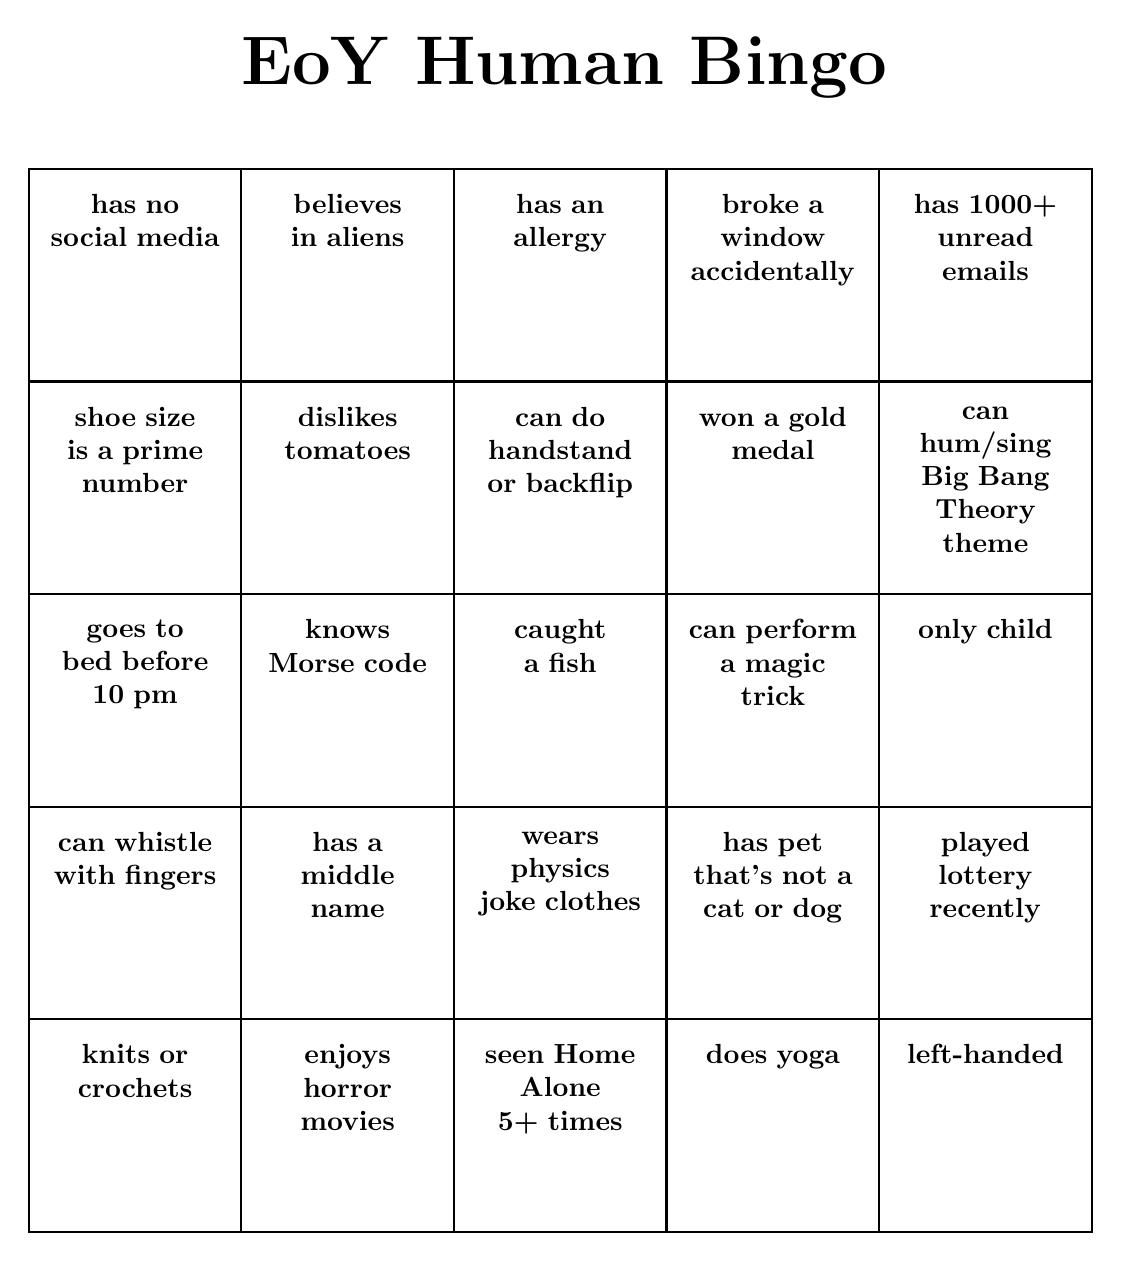
\begin{tikzpicture}
% Set the grid dimensions
\def\cellsize{2.7cm} % Each cell will be 2x2 cm

% Draw the grid and insert the numbers
\draw[thick] (0.0, 0.0) rectangle +(2.7, 2.7);
\node[anchor=north, align=center, text width=2.2cm] at (1.35, 2.5) {\textbf{has no social media}};
\draw[thick] (2.7, 0.0) rectangle +(2.7, 2.7);
\node[anchor=north, align=center, text width=2.2cm] at (4.050000000000001, 2.5) {\textbf{believes in aliens}};
\draw[thick] (5.4, 0.0) rectangle +(2.7, 2.7);
\node[anchor=north, align=center, text width=2.2cm] at (6.75, 2.5) {\textbf{has an allergy}};
\draw[thick] (8.100000000000001, 0.0) rectangle +(2.7, 2.7);
\node[anchor=north, align=center, text width=2.2cm] at (9.450000000000001, 2.5) {\textbf{broke a window accidentally}};
\draw[thick] (10.8, 0.0) rectangle +(2.7, 2.7);
\node[anchor=north, align=center, text width=2.2cm] at (12.15, 2.5) {\textbf{has 1000+ unread emails}};
\draw[thick] (0.0, -2.7) rectangle +(2.7, 2.7);
\node[anchor=north, align=center, text width=2.2cm] at (1.35, -0.2) {\textbf{shoe size is a prime number}};
\draw[thick] (2.7, -2.7) rectangle +(2.7, 2.7);
\node[anchor=north, align=center, text width=2.2cm] at (4.050000000000001, -0.2) {\textbf{dislikes tomatoes}};
\draw[thick] (5.4, -2.7) rectangle +(2.7, 2.7);
\node[anchor=north, align=center, text width=2.2cm] at (6.75, -0.2) {\textbf{can do handstand or backflip}};
\draw[thick] (8.100000000000001, -2.7) rectangle +(2.7, 2.7);
\node[anchor=north, align=center, text width=2.2cm] at (9.450000000000001, -0.2) {\textbf{won a gold medal}};
\draw[thick] (10.8, -2.7) rectangle +(2.7, 2.7);
\node[anchor=north, align=center, text width=2.2cm] at (12.15, -0.2) {\textbf{can hum/sing Big Bang Theory theme}};
\draw[thick] (0.0, -5.4) rectangle +(2.7, 2.7);
\node[anchor=north, align=center, text width=2.2cm] at (1.35, -2.9000000000000004) {\textbf{goes to bed before 10 pm}};
\draw[thick] (2.7, -5.4) rectangle +(2.7, 2.7);
\node[anchor=north, align=center, text width=2.2cm] at (4.050000000000001, -2.9000000000000004) {\textbf{knows Morse code}};
\draw[thick] (5.4, -5.4) rectangle +(2.7, 2.7);
\node[anchor=north, align=center, text width=2.2cm] at (6.75, -2.9000000000000004) {\textbf{caught a fish}};
\draw[thick] (8.100000000000001, -5.4) rectangle +(2.7, 2.7);
\node[anchor=north, align=center, text width=2.2cm] at (9.450000000000001, -2.9000000000000004) {\textbf{can perform a magic trick}};
\draw[thick] (10.8, -5.4) rectangle +(2.7, 2.7);
\node[anchor=north, align=center, text width=2.2cm] at (12.15, -2.9000000000000004) {\textbf{only child}};
\draw[thick] (0.0, -8.100000000000001) rectangle +(2.7, 2.7);
\node[anchor=north, align=center, text width=2.2cm] at (1.35, -5.600000000000001) {\textbf{can whistle with fingers}};
\draw[thick] (2.7, -8.100000000000001) rectangle +(2.7, 2.7);
\node[anchor=north, align=center, text width=2.2cm] at (4.050000000000001, -5.600000000000001) {\textbf{has a middle name}};
\draw[thick] (5.4, -8.100000000000001) rectangle +(2.7, 2.7);
\node[anchor=north, align=center, text width=2.2cm] at (6.75, -5.600000000000001) {\textbf{wears physics joke clothes}};
\draw[thick] (8.100000000000001, -8.100000000000001) rectangle +(2.7, 2.7);
\node[anchor=north, align=center, text width=2.2cm] at (9.450000000000001, -5.600000000000001) {\textbf{has pet that's not a cat or dog}};
\draw[thick] (10.8, -8.100000000000001) rectangle +(2.7, 2.7);
\node[anchor=north, align=center, text width=2.2cm] at (12.15, -5.600000000000001) {\textbf{played lottery recently}};
\draw[thick] (0.0, -10.8) rectangle +(2.7, 2.7);
\node[anchor=north, align=center, text width=2.2cm] at (1.35, -8.3) {\textbf{knits or crochets}};
\draw[thick] (2.7, -10.8) rectangle +(2.7, 2.7);
\node[anchor=north, align=center, text width=2.2cm] at (4.050000000000001, -8.3) {\textbf{enjoys horror movies}};
\draw[thick] (5.4, -10.8) rectangle +(2.7, 2.7);
\node[anchor=north, align=center, text width=2.2cm] at (6.75, -8.3) {\textbf{seen Home Alone 5+ times}};
\draw[thick] (8.100000000000001, -10.8) rectangle +(2.7, 2.7);
\node[anchor=north, align=center, text width=2.2cm] at (9.450000000000001, -8.3) {\textbf{does yoga}};
\draw[thick] (10.8, -10.8) rectangle +(2.7, 2.7);
\node[anchor=north, align=center, text width=2.2cm] at (12.15, -8.3) {\textbf{left-handed}};
\node[anchor=north, font = \Huge] at (6.8, 4.5){\textbf{EoY Human Bingo}};
\end{tikzpicture}
\end{center}
\newpage\begin{center}
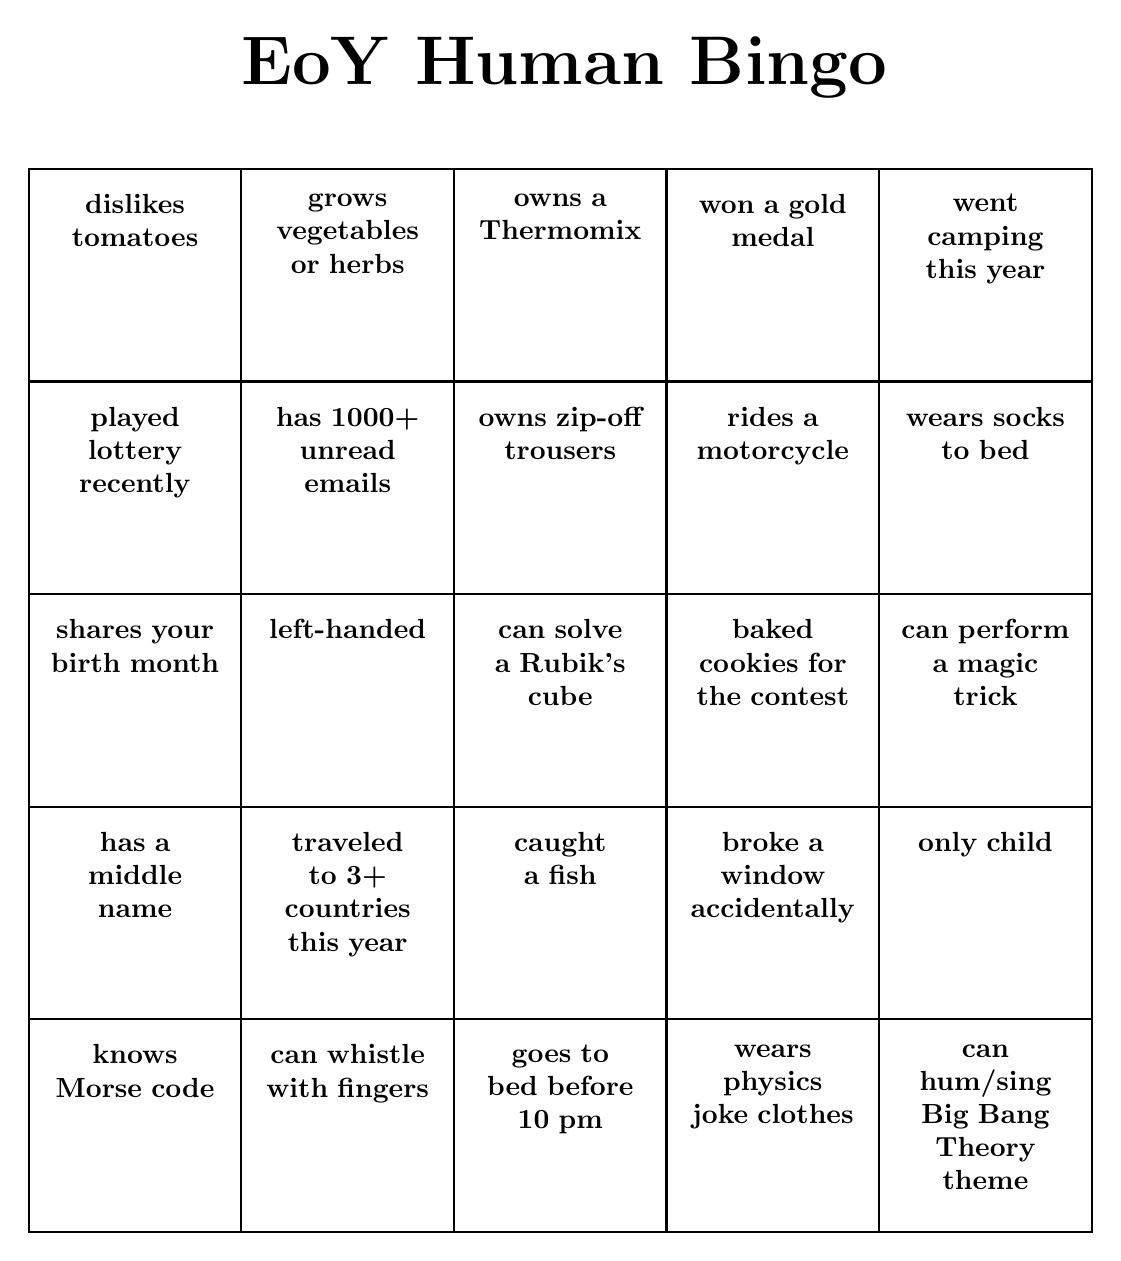
\begin{tikzpicture}
% Set the grid dimensions
\def\cellsize{2.7cm} % Each cell will be 2x2 cm

% Draw the grid and insert the numbers
\draw[thick] (0.0, 0.0) rectangle +(2.7, 2.7);
\node[anchor=north, align=center, text width=2.2cm] at (1.35, 2.5) {\textbf{dislikes tomatoes}};
\draw[thick] (2.7, 0.0) rectangle +(2.7, 2.7);
\node[anchor=north, align=center, text width=2.2cm] at (4.050000000000001, 2.5) {\textbf{grows vegetables or herbs}};
\draw[thick] (5.4, 0.0) rectangle +(2.7, 2.7);
\node[anchor=north, align=center, text width=2.2cm] at (6.75, 2.5) {\textbf{owns a Thermomix}};
\draw[thick] (8.100000000000001, 0.0) rectangle +(2.7, 2.7);
\node[anchor=north, align=center, text width=2.2cm] at (9.450000000000001, 2.5) {\textbf{won a gold medal}};
\draw[thick] (10.8, 0.0) rectangle +(2.7, 2.7);
\node[anchor=north, align=center, text width=2.2cm] at (12.15, 2.5) {\textbf{went camping this year}};
\draw[thick] (0.0, -2.7) rectangle +(2.7, 2.7);
\node[anchor=north, align=center, text width=2.2cm] at (1.35, -0.2) {\textbf{played lottery recently}};
\draw[thick] (2.7, -2.7) rectangle +(2.7, 2.7);
\node[anchor=north, align=center, text width=2.2cm] at (4.050000000000001, -0.2) {\textbf{has 1000+ unread emails}};
\draw[thick] (5.4, -2.7) rectangle +(2.7, 2.7);
\node[anchor=north, align=center, text width=2.2cm] at (6.75, -0.2) {\textbf{owns zip-off trousers}};
\draw[thick] (8.100000000000001, -2.7) rectangle +(2.7, 2.7);
\node[anchor=north, align=center, text width=2.2cm] at (9.450000000000001, -0.2) {\textbf{rides a motorcycle}};
\draw[thick] (10.8, -2.7) rectangle +(2.7, 2.7);
\node[anchor=north, align=center, text width=2.2cm] at (12.15, -0.2) {\textbf{wears socks to bed}};
\draw[thick] (0.0, -5.4) rectangle +(2.7, 2.7);
\node[anchor=north, align=center, text width=2.2cm] at (1.35, -2.9000000000000004) {\textbf{shares your birth month}};
\draw[thick] (2.7, -5.4) rectangle +(2.7, 2.7);
\node[anchor=north, align=center, text width=2.2cm] at (4.050000000000001, -2.9000000000000004) {\textbf{left-handed}};
\draw[thick] (5.4, -5.4) rectangle +(2.7, 2.7);
\node[anchor=north, align=center, text width=2.2cm] at (6.75, -2.9000000000000004) {\textbf{can solve a Rubik's cube}};
\draw[thick] (8.100000000000001, -5.4) rectangle +(2.7, 2.7);
\node[anchor=north, align=center, text width=2.2cm] at (9.450000000000001, -2.9000000000000004) {\textbf{baked cookies for the contest}};
\draw[thick] (10.8, -5.4) rectangle +(2.7, 2.7);
\node[anchor=north, align=center, text width=2.2cm] at (12.15, -2.9000000000000004) {\textbf{can perform a magic trick}};
\draw[thick] (0.0, -8.100000000000001) rectangle +(2.7, 2.7);
\node[anchor=north, align=center, text width=2.2cm] at (1.35, -5.600000000000001) {\textbf{has a middle name}};
\draw[thick] (2.7, -8.100000000000001) rectangle +(2.7, 2.7);
\node[anchor=north, align=center, text width=2.2cm] at (4.050000000000001, -5.600000000000001) {\textbf{traveled to 3+ countries this year}};
\draw[thick] (5.4, -8.100000000000001) rectangle +(2.7, 2.7);
\node[anchor=north, align=center, text width=2.2cm] at (6.75, -5.600000000000001) {\textbf{caught a fish}};
\draw[thick] (8.100000000000001, -8.100000000000001) rectangle +(2.7, 2.7);
\node[anchor=north, align=center, text width=2.2cm] at (9.450000000000001, -5.600000000000001) {\textbf{broke a window accidentally}};
\draw[thick] (10.8, -8.100000000000001) rectangle +(2.7, 2.7);
\node[anchor=north, align=center, text width=2.2cm] at (12.15, -5.600000000000001) {\textbf{only child}};
\draw[thick] (0.0, -10.8) rectangle +(2.7, 2.7);
\node[anchor=north, align=center, text width=2.2cm] at (1.35, -8.3) {\textbf{knows Morse code}};
\draw[thick] (2.7, -10.8) rectangle +(2.7, 2.7);
\node[anchor=north, align=center, text width=2.2cm] at (4.050000000000001, -8.3) {\textbf{can whistle with fingers}};
\draw[thick] (5.4, -10.8) rectangle +(2.7, 2.7);
\node[anchor=north, align=center, text width=2.2cm] at (6.75, -8.3) {\textbf{goes to bed before 10 pm}};
\draw[thick] (8.100000000000001, -10.8) rectangle +(2.7, 2.7);
\node[anchor=north, align=center, text width=2.2cm] at (9.450000000000001, -8.3) {\textbf{wears physics joke clothes}};
\draw[thick] (10.8, -10.8) rectangle +(2.7, 2.7);
\node[anchor=north, align=center, text width=2.2cm] at (12.15, -8.3) {\textbf{can hum/sing Big Bang Theory theme}};
\node[anchor=north, font = \Huge] at (6.8, 4.5){\textbf{EoY Human Bingo}};
\end{tikzpicture}
\end{center}
\newpage\begin{center}
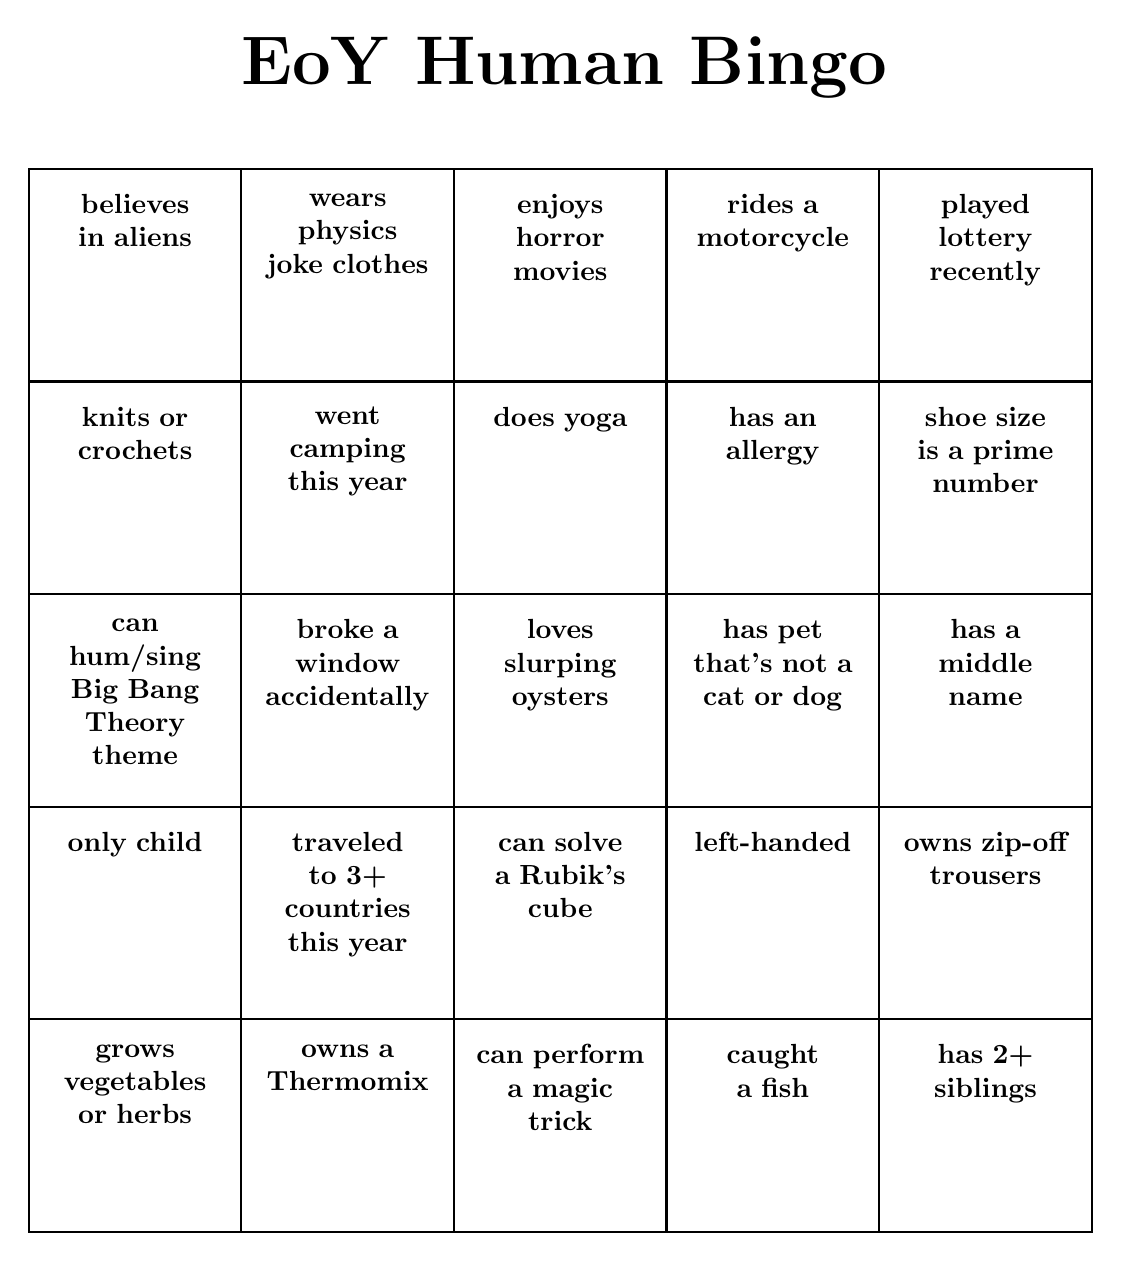
\begin{tikzpicture}
% Set the grid dimensions
\def\cellsize{2.7cm} % Each cell will be 2x2 cm

% Draw the grid and insert the numbers
\draw[thick] (0.0, 0.0) rectangle +(2.7, 2.7);
\node[anchor=north, align=center, text width=2.2cm] at (1.35, 2.5) {\textbf{believes in aliens}};
\draw[thick] (2.7, 0.0) rectangle +(2.7, 2.7);
\node[anchor=north, align=center, text width=2.2cm] at (4.050000000000001, 2.5) {\textbf{wears physics joke clothes}};
\draw[thick] (5.4, 0.0) rectangle +(2.7, 2.7);
\node[anchor=north, align=center, text width=2.2cm] at (6.75, 2.5) {\textbf{enjoys horror movies}};
\draw[thick] (8.100000000000001, 0.0) rectangle +(2.7, 2.7);
\node[anchor=north, align=center, text width=2.2cm] at (9.450000000000001, 2.5) {\textbf{rides a motorcycle}};
\draw[thick] (10.8, 0.0) rectangle +(2.7, 2.7);
\node[anchor=north, align=center, text width=2.2cm] at (12.15, 2.5) {\textbf{played lottery recently}};
\draw[thick] (0.0, -2.7) rectangle +(2.7, 2.7);
\node[anchor=north, align=center, text width=2.2cm] at (1.35, -0.2) {\textbf{knits or crochets}};
\draw[thick] (2.7, -2.7) rectangle +(2.7, 2.7);
\node[anchor=north, align=center, text width=2.2cm] at (4.050000000000001, -0.2) {\textbf{went camping this year}};
\draw[thick] (5.4, -2.7) rectangle +(2.7, 2.7);
\node[anchor=north, align=center, text width=2.2cm] at (6.75, -0.2) {\textbf{does yoga}};
\draw[thick] (8.100000000000001, -2.7) rectangle +(2.7, 2.7);
\node[anchor=north, align=center, text width=2.2cm] at (9.450000000000001, -0.2) {\textbf{has an allergy}};
\draw[thick] (10.8, -2.7) rectangle +(2.7, 2.7);
\node[anchor=north, align=center, text width=2.2cm] at (12.15, -0.2) {\textbf{shoe size is a prime number}};
\draw[thick] (0.0, -5.4) rectangle +(2.7, 2.7);
\node[anchor=north, align=center, text width=2.2cm] at (1.35, -2.9000000000000004) {\textbf{can hum/sing Big Bang Theory theme}};
\draw[thick] (2.7, -5.4) rectangle +(2.7, 2.7);
\node[anchor=north, align=center, text width=2.2cm] at (4.050000000000001, -2.9000000000000004) {\textbf{broke a window accidentally}};
\draw[thick] (5.4, -5.4) rectangle +(2.7, 2.7);
\node[anchor=north, align=center, text width=2.2cm] at (6.75, -2.9000000000000004) {\textbf{loves slurping oysters}};
\draw[thick] (8.100000000000001, -5.4) rectangle +(2.7, 2.7);
\node[anchor=north, align=center, text width=2.2cm] at (9.450000000000001, -2.9000000000000004) {\textbf{has pet that's not a cat or dog}};
\draw[thick] (10.8, -5.4) rectangle +(2.7, 2.7);
\node[anchor=north, align=center, text width=2.2cm] at (12.15, -2.9000000000000004) {\textbf{has a middle name}};
\draw[thick] (0.0, -8.100000000000001) rectangle +(2.7, 2.7);
\node[anchor=north, align=center, text width=2.2cm] at (1.35, -5.600000000000001) {\textbf{only child}};
\draw[thick] (2.7, -8.100000000000001) rectangle +(2.7, 2.7);
\node[anchor=north, align=center, text width=2.2cm] at (4.050000000000001, -5.600000000000001) {\textbf{traveled to 3+ countries this year}};
\draw[thick] (5.4, -8.100000000000001) rectangle +(2.7, 2.7);
\node[anchor=north, align=center, text width=2.2cm] at (6.75, -5.600000000000001) {\textbf{can solve a Rubik's cube}};
\draw[thick] (8.100000000000001, -8.100000000000001) rectangle +(2.7, 2.7);
\node[anchor=north, align=center, text width=2.2cm] at (9.450000000000001, -5.600000000000001) {\textbf{left-handed}};
\draw[thick] (10.8, -8.100000000000001) rectangle +(2.7, 2.7);
\node[anchor=north, align=center, text width=2.2cm] at (12.15, -5.600000000000001) {\textbf{owns zip-off trousers}};
\draw[thick] (0.0, -10.8) rectangle +(2.7, 2.7);
\node[anchor=north, align=center, text width=2.2cm] at (1.35, -8.3) {\textbf{grows vegetables or herbs}};
\draw[thick] (2.7, -10.8) rectangle +(2.7, 2.7);
\node[anchor=north, align=center, text width=2.2cm] at (4.050000000000001, -8.3) {\textbf{owns a Thermomix}};
\draw[thick] (5.4, -10.8) rectangle +(2.7, 2.7);
\node[anchor=north, align=center, text width=2.2cm] at (6.75, -8.3) {\textbf{can perform a magic trick}};
\draw[thick] (8.100000000000001, -10.8) rectangle +(2.7, 2.7);
\node[anchor=north, align=center, text width=2.2cm] at (9.450000000000001, -8.3) {\textbf{caught a fish}};
\draw[thick] (10.8, -10.8) rectangle +(2.7, 2.7);
\node[anchor=north, align=center, text width=2.2cm] at (12.15, -8.3) {\textbf{has 2+ siblings}};
\node[anchor=north, font = \Huge] at (6.8, 4.5){\textbf{EoY Human Bingo}};
\end{tikzpicture}
\end{center}
\newpage\begin{center}
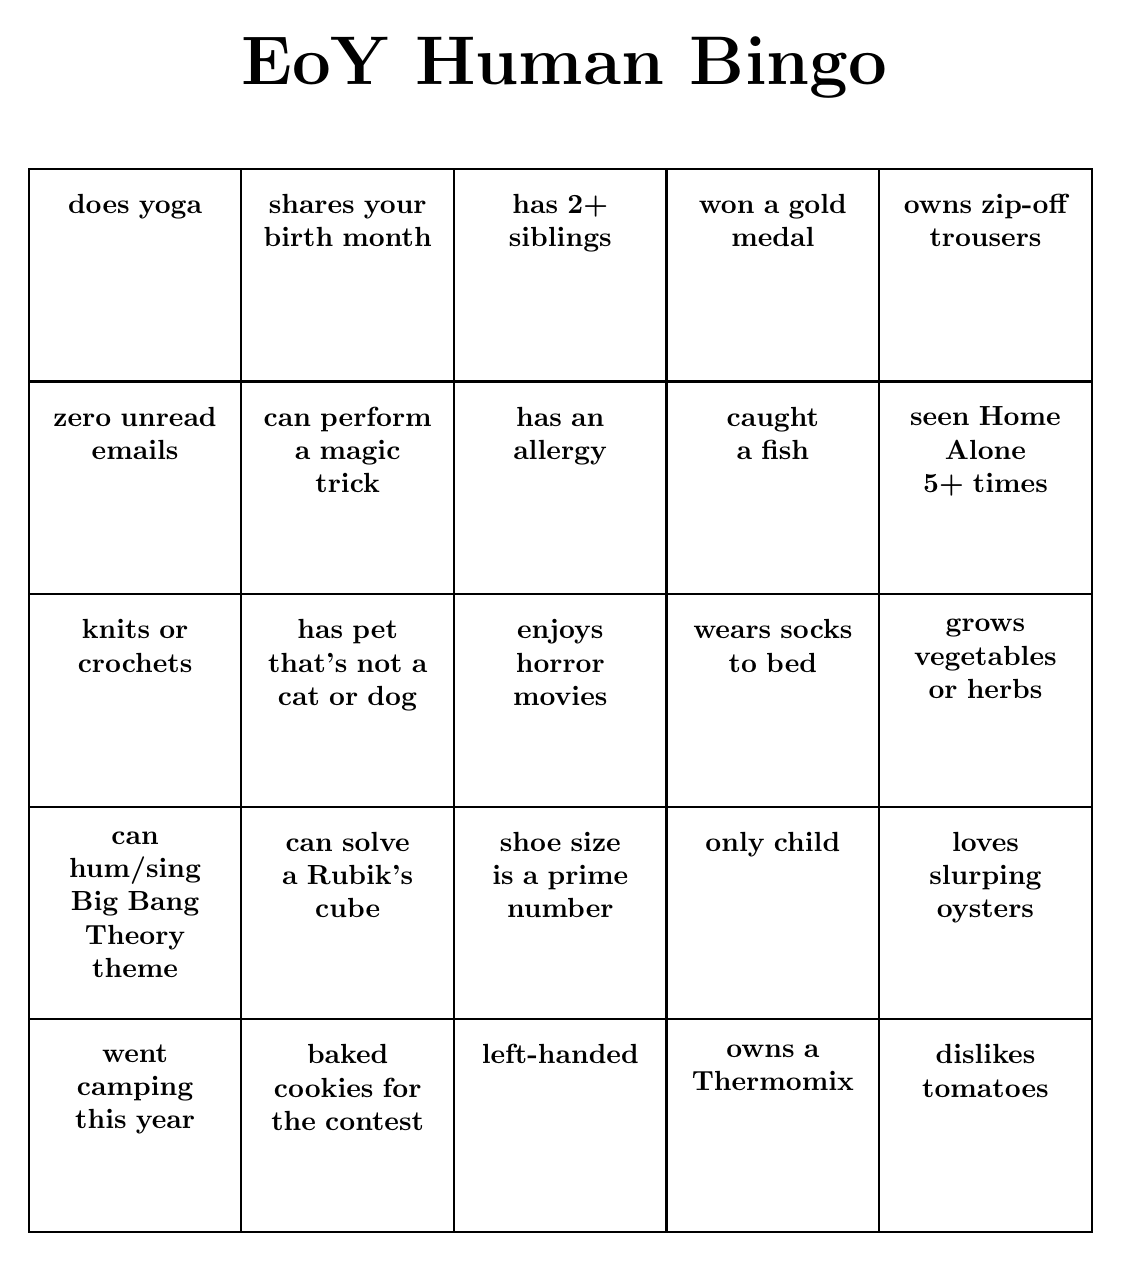
\begin{tikzpicture}
% Set the grid dimensions
\def\cellsize{2.7cm} % Each cell will be 2x2 cm

% Draw the grid and insert the numbers
\draw[thick] (0.0, 0.0) rectangle +(2.7, 2.7);
\node[anchor=north, align=center, text width=2.2cm] at (1.35, 2.5) {\textbf{does yoga}};
\draw[thick] (2.7, 0.0) rectangle +(2.7, 2.7);
\node[anchor=north, align=center, text width=2.2cm] at (4.050000000000001, 2.5) {\textbf{shares your birth month}};
\draw[thick] (5.4, 0.0) rectangle +(2.7, 2.7);
\node[anchor=north, align=center, text width=2.2cm] at (6.75, 2.5) {\textbf{has 2+ siblings}};
\draw[thick] (8.100000000000001, 0.0) rectangle +(2.7, 2.7);
\node[anchor=north, align=center, text width=2.2cm] at (9.450000000000001, 2.5) {\textbf{won a gold medal}};
\draw[thick] (10.8, 0.0) rectangle +(2.7, 2.7);
\node[anchor=north, align=center, text width=2.2cm] at (12.15, 2.5) {\textbf{owns zip-off trousers}};
\draw[thick] (0.0, -2.7) rectangle +(2.7, 2.7);
\node[anchor=north, align=center, text width=2.2cm] at (1.35, -0.2) {\textbf{zero unread emails}};
\draw[thick] (2.7, -2.7) rectangle +(2.7, 2.7);
\node[anchor=north, align=center, text width=2.2cm] at (4.050000000000001, -0.2) {\textbf{can perform a magic trick}};
\draw[thick] (5.4, -2.7) rectangle +(2.7, 2.7);
\node[anchor=north, align=center, text width=2.2cm] at (6.75, -0.2) {\textbf{has an allergy}};
\draw[thick] (8.100000000000001, -2.7) rectangle +(2.7, 2.7);
\node[anchor=north, align=center, text width=2.2cm] at (9.450000000000001, -0.2) {\textbf{caught a fish}};
\draw[thick] (10.8, -2.7) rectangle +(2.7, 2.7);
\node[anchor=north, align=center, text width=2.2cm] at (12.15, -0.2) {\textbf{seen Home Alone 5+ times}};
\draw[thick] (0.0, -5.4) rectangle +(2.7, 2.7);
\node[anchor=north, align=center, text width=2.2cm] at (1.35, -2.9000000000000004) {\textbf{knits or crochets}};
\draw[thick] (2.7, -5.4) rectangle +(2.7, 2.7);
\node[anchor=north, align=center, text width=2.2cm] at (4.050000000000001, -2.9000000000000004) {\textbf{has pet that's not a cat or dog}};
\draw[thick] (5.4, -5.4) rectangle +(2.7, 2.7);
\node[anchor=north, align=center, text width=2.2cm] at (6.75, -2.9000000000000004) {\textbf{enjoys horror movies}};
\draw[thick] (8.100000000000001, -5.4) rectangle +(2.7, 2.7);
\node[anchor=north, align=center, text width=2.2cm] at (9.450000000000001, -2.9000000000000004) {\textbf{wears socks to bed}};
\draw[thick] (10.8, -5.4) rectangle +(2.7, 2.7);
\node[anchor=north, align=center, text width=2.2cm] at (12.15, -2.9000000000000004) {\textbf{grows vegetables or herbs}};
\draw[thick] (0.0, -8.100000000000001) rectangle +(2.7, 2.7);
\node[anchor=north, align=center, text width=2.2cm] at (1.35, -5.600000000000001) {\textbf{can hum/sing Big Bang Theory theme}};
\draw[thick] (2.7, -8.100000000000001) rectangle +(2.7, 2.7);
\node[anchor=north, align=center, text width=2.2cm] at (4.050000000000001, -5.600000000000001) {\textbf{can solve a Rubik's cube}};
\draw[thick] (5.4, -8.100000000000001) rectangle +(2.7, 2.7);
\node[anchor=north, align=center, text width=2.2cm] at (6.75, -5.600000000000001) {\textbf{shoe size is a prime number}};
\draw[thick] (8.100000000000001, -8.100000000000001) rectangle +(2.7, 2.7);
\node[anchor=north, align=center, text width=2.2cm] at (9.450000000000001, -5.600000000000001) {\textbf{only child}};
\draw[thick] (10.8, -8.100000000000001) rectangle +(2.7, 2.7);
\node[anchor=north, align=center, text width=2.2cm] at (12.15, -5.600000000000001) {\textbf{loves slurping oysters}};
\draw[thick] (0.0, -10.8) rectangle +(2.7, 2.7);
\node[anchor=north, align=center, text width=2.2cm] at (1.35, -8.3) {\textbf{went camping this year}};
\draw[thick] (2.7, -10.8) rectangle +(2.7, 2.7);
\node[anchor=north, align=center, text width=2.2cm] at (4.050000000000001, -8.3) {\textbf{baked cookies for the contest}};
\draw[thick] (5.4, -10.8) rectangle +(2.7, 2.7);
\node[anchor=north, align=center, text width=2.2cm] at (6.75, -8.3) {\textbf{left-handed}};
\draw[thick] (8.100000000000001, -10.8) rectangle +(2.7, 2.7);
\node[anchor=north, align=center, text width=2.2cm] at (9.450000000000001, -8.3) {\textbf{owns a Thermomix}};
\draw[thick] (10.8, -10.8) rectangle +(2.7, 2.7);
\node[anchor=north, align=center, text width=2.2cm] at (12.15, -8.3) {\textbf{dislikes tomatoes}};
\node[anchor=north, font = \Huge] at (6.8, 4.5){\textbf{EoY Human Bingo}};
\end{tikzpicture}
\end{center}
\newpage\begin{center}
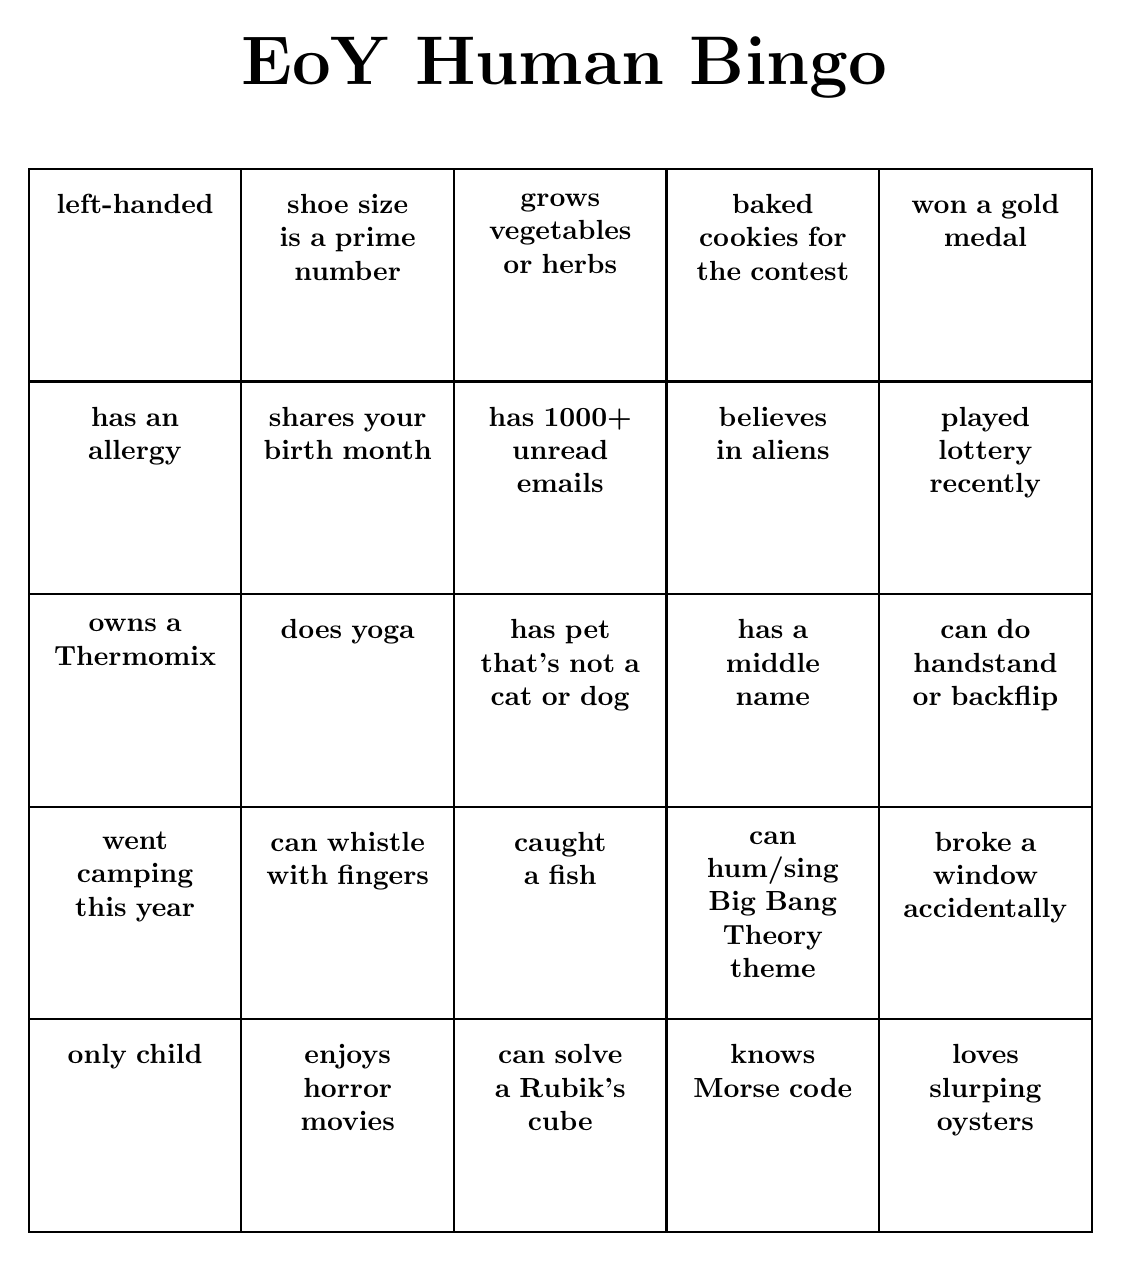
\begin{tikzpicture}
% Set the grid dimensions
\def\cellsize{2.7cm} % Each cell will be 2x2 cm

% Draw the grid and insert the numbers
\draw[thick] (0.0, 0.0) rectangle +(2.7, 2.7);
\node[anchor=north, align=center, text width=2.2cm] at (1.35, 2.5) {\textbf{left-handed}};
\draw[thick] (2.7, 0.0) rectangle +(2.7, 2.7);
\node[anchor=north, align=center, text width=2.2cm] at (4.050000000000001, 2.5) {\textbf{shoe size is a prime number}};
\draw[thick] (5.4, 0.0) rectangle +(2.7, 2.7);
\node[anchor=north, align=center, text width=2.2cm] at (6.75, 2.5) {\textbf{grows vegetables or herbs}};
\draw[thick] (8.100000000000001, 0.0) rectangle +(2.7, 2.7);
\node[anchor=north, align=center, text width=2.2cm] at (9.450000000000001, 2.5) {\textbf{baked cookies for the contest}};
\draw[thick] (10.8, 0.0) rectangle +(2.7, 2.7);
\node[anchor=north, align=center, text width=2.2cm] at (12.15, 2.5) {\textbf{won a gold medal}};
\draw[thick] (0.0, -2.7) rectangle +(2.7, 2.7);
\node[anchor=north, align=center, text width=2.2cm] at (1.35, -0.2) {\textbf{has an allergy}};
\draw[thick] (2.7, -2.7) rectangle +(2.7, 2.7);
\node[anchor=north, align=center, text width=2.2cm] at (4.050000000000001, -0.2) {\textbf{shares your birth month}};
\draw[thick] (5.4, -2.7) rectangle +(2.7, 2.7);
\node[anchor=north, align=center, text width=2.2cm] at (6.75, -0.2) {\textbf{has 1000+ unread emails}};
\draw[thick] (8.100000000000001, -2.7) rectangle +(2.7, 2.7);
\node[anchor=north, align=center, text width=2.2cm] at (9.450000000000001, -0.2) {\textbf{believes in aliens}};
\draw[thick] (10.8, -2.7) rectangle +(2.7, 2.7);
\node[anchor=north, align=center, text width=2.2cm] at (12.15, -0.2) {\textbf{played lottery recently}};
\draw[thick] (0.0, -5.4) rectangle +(2.7, 2.7);
\node[anchor=north, align=center, text width=2.2cm] at (1.35, -2.9000000000000004) {\textbf{owns a Thermomix}};
\draw[thick] (2.7, -5.4) rectangle +(2.7, 2.7);
\node[anchor=north, align=center, text width=2.2cm] at (4.050000000000001, -2.9000000000000004) {\textbf{does yoga}};
\draw[thick] (5.4, -5.4) rectangle +(2.7, 2.7);
\node[anchor=north, align=center, text width=2.2cm] at (6.75, -2.9000000000000004) {\textbf{has pet that's not a cat or dog}};
\draw[thick] (8.100000000000001, -5.4) rectangle +(2.7, 2.7);
\node[anchor=north, align=center, text width=2.2cm] at (9.450000000000001, -2.9000000000000004) {\textbf{has a middle name}};
\draw[thick] (10.8, -5.4) rectangle +(2.7, 2.7);
\node[anchor=north, align=center, text width=2.2cm] at (12.15, -2.9000000000000004) {\textbf{can do handstand or backflip}};
\draw[thick] (0.0, -8.100000000000001) rectangle +(2.7, 2.7);
\node[anchor=north, align=center, text width=2.2cm] at (1.35, -5.600000000000001) {\textbf{went camping this year}};
\draw[thick] (2.7, -8.100000000000001) rectangle +(2.7, 2.7);
\node[anchor=north, align=center, text width=2.2cm] at (4.050000000000001, -5.600000000000001) {\textbf{can whistle with fingers}};
\draw[thick] (5.4, -8.100000000000001) rectangle +(2.7, 2.7);
\node[anchor=north, align=center, text width=2.2cm] at (6.75, -5.600000000000001) {\textbf{caught a fish}};
\draw[thick] (8.100000000000001, -8.100000000000001) rectangle +(2.7, 2.7);
\node[anchor=north, align=center, text width=2.2cm] at (9.450000000000001, -5.600000000000001) {\textbf{can hum/sing Big Bang Theory theme}};
\draw[thick] (10.8, -8.100000000000001) rectangle +(2.7, 2.7);
\node[anchor=north, align=center, text width=2.2cm] at (12.15, -5.600000000000001) {\textbf{broke a window accidentally}};
\draw[thick] (0.0, -10.8) rectangle +(2.7, 2.7);
\node[anchor=north, align=center, text width=2.2cm] at (1.35, -8.3) {\textbf{only child}};
\draw[thick] (2.7, -10.8) rectangle +(2.7, 2.7);
\node[anchor=north, align=center, text width=2.2cm] at (4.050000000000001, -8.3) {\textbf{enjoys horror movies}};
\draw[thick] (5.4, -10.8) rectangle +(2.7, 2.7);
\node[anchor=north, align=center, text width=2.2cm] at (6.75, -8.3) {\textbf{can solve a Rubik's cube}};
\draw[thick] (8.100000000000001, -10.8) rectangle +(2.7, 2.7);
\node[anchor=north, align=center, text width=2.2cm] at (9.450000000000001, -8.3) {\textbf{knows Morse code}};
\draw[thick] (10.8, -10.8) rectangle +(2.7, 2.7);
\node[anchor=north, align=center, text width=2.2cm] at (12.15, -8.3) {\textbf{loves slurping oysters}};
\node[anchor=north, font = \Huge] at (6.8, 4.5){\textbf{EoY Human Bingo}};
\end{tikzpicture}
\end{center}
\newpage\begin{center}
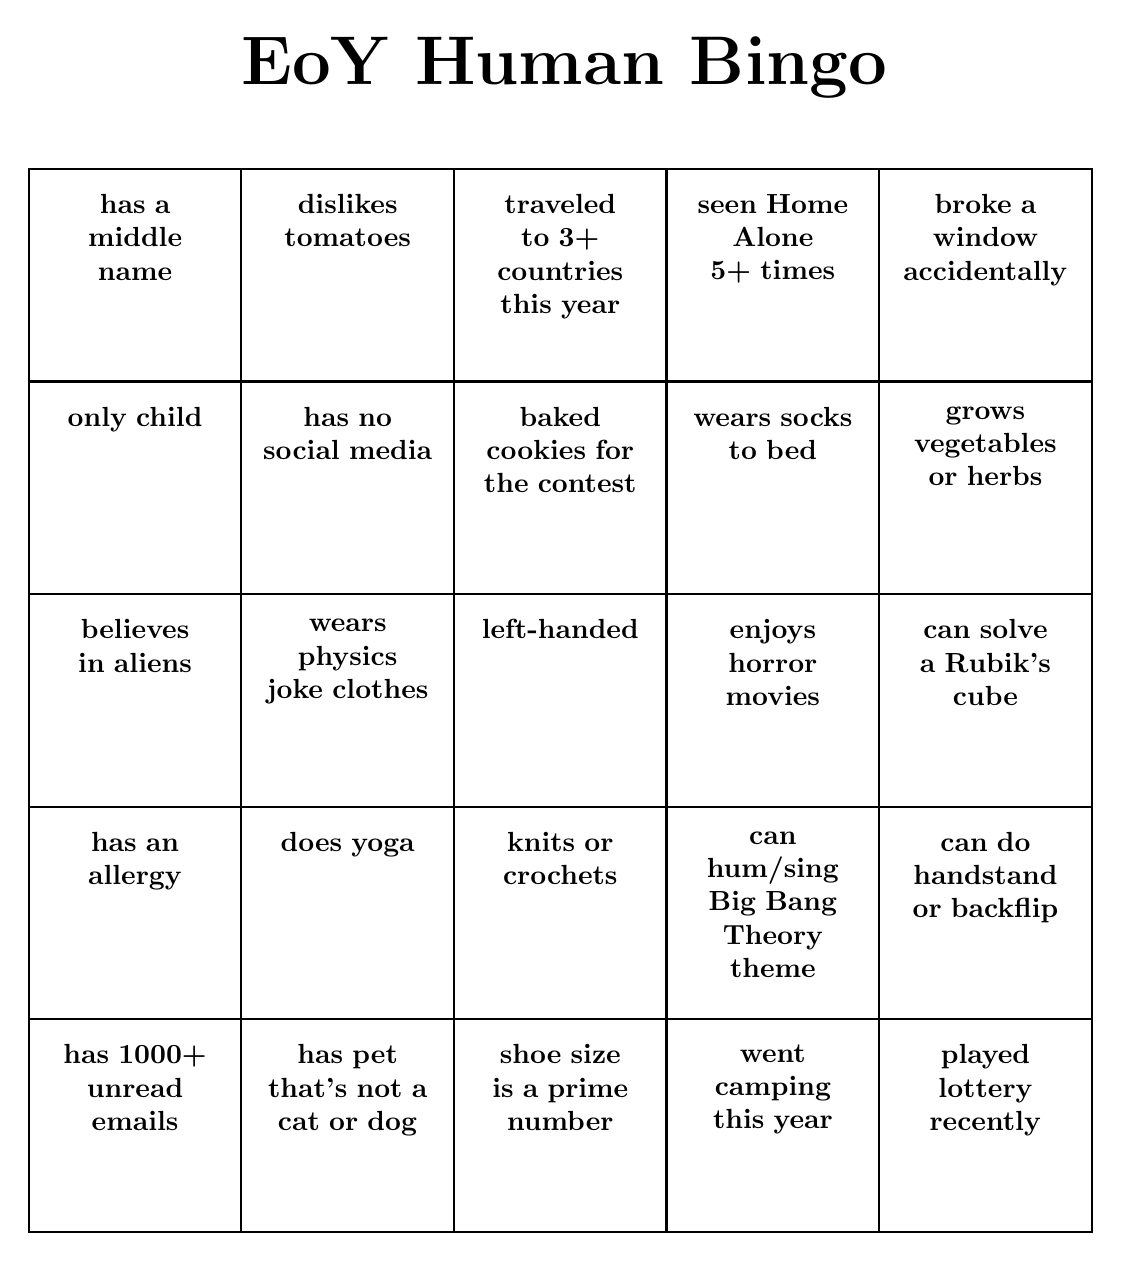
\begin{tikzpicture}
% Set the grid dimensions
\def\cellsize{2.7cm} % Each cell will be 2x2 cm

% Draw the grid and insert the numbers
\draw[thick] (0.0, 0.0) rectangle +(2.7, 2.7);
\node[anchor=north, align=center, text width=2.2cm] at (1.35, 2.5) {\textbf{has a middle name}};
\draw[thick] (2.7, 0.0) rectangle +(2.7, 2.7);
\node[anchor=north, align=center, text width=2.2cm] at (4.050000000000001, 2.5) {\textbf{dislikes tomatoes}};
\draw[thick] (5.4, 0.0) rectangle +(2.7, 2.7);
\node[anchor=north, align=center, text width=2.2cm] at (6.75, 2.5) {\textbf{traveled to 3+ countries this year}};
\draw[thick] (8.100000000000001, 0.0) rectangle +(2.7, 2.7);
\node[anchor=north, align=center, text width=2.2cm] at (9.450000000000001, 2.5) {\textbf{seen Home Alone 5+ times}};
\draw[thick] (10.8, 0.0) rectangle +(2.7, 2.7);
\node[anchor=north, align=center, text width=2.2cm] at (12.15, 2.5) {\textbf{broke a window accidentally}};
\draw[thick] (0.0, -2.7) rectangle +(2.7, 2.7);
\node[anchor=north, align=center, text width=2.2cm] at (1.35, -0.2) {\textbf{only child}};
\draw[thick] (2.7, -2.7) rectangle +(2.7, 2.7);
\node[anchor=north, align=center, text width=2.2cm] at (4.050000000000001, -0.2) {\textbf{has no social media}};
\draw[thick] (5.4, -2.7) rectangle +(2.7, 2.7);
\node[anchor=north, align=center, text width=2.2cm] at (6.75, -0.2) {\textbf{baked cookies for the contest}};
\draw[thick] (8.100000000000001, -2.7) rectangle +(2.7, 2.7);
\node[anchor=north, align=center, text width=2.2cm] at (9.450000000000001, -0.2) {\textbf{wears socks to bed}};
\draw[thick] (10.8, -2.7) rectangle +(2.7, 2.7);
\node[anchor=north, align=center, text width=2.2cm] at (12.15, -0.2) {\textbf{grows vegetables or herbs}};
\draw[thick] (0.0, -5.4) rectangle +(2.7, 2.7);
\node[anchor=north, align=center, text width=2.2cm] at (1.35, -2.9000000000000004) {\textbf{believes in aliens}};
\draw[thick] (2.7, -5.4) rectangle +(2.7, 2.7);
\node[anchor=north, align=center, text width=2.2cm] at (4.050000000000001, -2.9000000000000004) {\textbf{wears physics joke clothes}};
\draw[thick] (5.4, -5.4) rectangle +(2.7, 2.7);
\node[anchor=north, align=center, text width=2.2cm] at (6.75, -2.9000000000000004) {\textbf{left-handed}};
\draw[thick] (8.100000000000001, -5.4) rectangle +(2.7, 2.7);
\node[anchor=north, align=center, text width=2.2cm] at (9.450000000000001, -2.9000000000000004) {\textbf{enjoys horror movies}};
\draw[thick] (10.8, -5.4) rectangle +(2.7, 2.7);
\node[anchor=north, align=center, text width=2.2cm] at (12.15, -2.9000000000000004) {\textbf{can solve a Rubik's cube}};
\draw[thick] (0.0, -8.100000000000001) rectangle +(2.7, 2.7);
\node[anchor=north, align=center, text width=2.2cm] at (1.35, -5.600000000000001) {\textbf{has an allergy}};
\draw[thick] (2.7, -8.100000000000001) rectangle +(2.7, 2.7);
\node[anchor=north, align=center, text width=2.2cm] at (4.050000000000001, -5.600000000000001) {\textbf{does yoga}};
\draw[thick] (5.4, -8.100000000000001) rectangle +(2.7, 2.7);
\node[anchor=north, align=center, text width=2.2cm] at (6.75, -5.600000000000001) {\textbf{knits or crochets}};
\draw[thick] (8.100000000000001, -8.100000000000001) rectangle +(2.7, 2.7);
\node[anchor=north, align=center, text width=2.2cm] at (9.450000000000001, -5.600000000000001) {\textbf{can hum/sing Big Bang Theory theme}};
\draw[thick] (10.8, -8.100000000000001) rectangle +(2.7, 2.7);
\node[anchor=north, align=center, text width=2.2cm] at (12.15, -5.600000000000001) {\textbf{can do handstand or backflip}};
\draw[thick] (0.0, -10.8) rectangle +(2.7, 2.7);
\node[anchor=north, align=center, text width=2.2cm] at (1.35, -8.3) {\textbf{has 1000+ unread emails}};
\draw[thick] (2.7, -10.8) rectangle +(2.7, 2.7);
\node[anchor=north, align=center, text width=2.2cm] at (4.050000000000001, -8.3) {\textbf{has pet that's not a cat or dog}};
\draw[thick] (5.4, -10.8) rectangle +(2.7, 2.7);
\node[anchor=north, align=center, text width=2.2cm] at (6.75, -8.3) {\textbf{shoe size is a prime number}};
\draw[thick] (8.100000000000001, -10.8) rectangle +(2.7, 2.7);
\node[anchor=north, align=center, text width=2.2cm] at (9.450000000000001, -8.3) {\textbf{went camping this year}};
\draw[thick] (10.8, -10.8) rectangle +(2.7, 2.7);
\node[anchor=north, align=center, text width=2.2cm] at (12.15, -8.3) {\textbf{played lottery recently}};
\node[anchor=north, font = \Huge] at (6.8, 4.5){\textbf{EoY Human Bingo}};
\end{tikzpicture}
\end{center}
\newpage\begin{center}
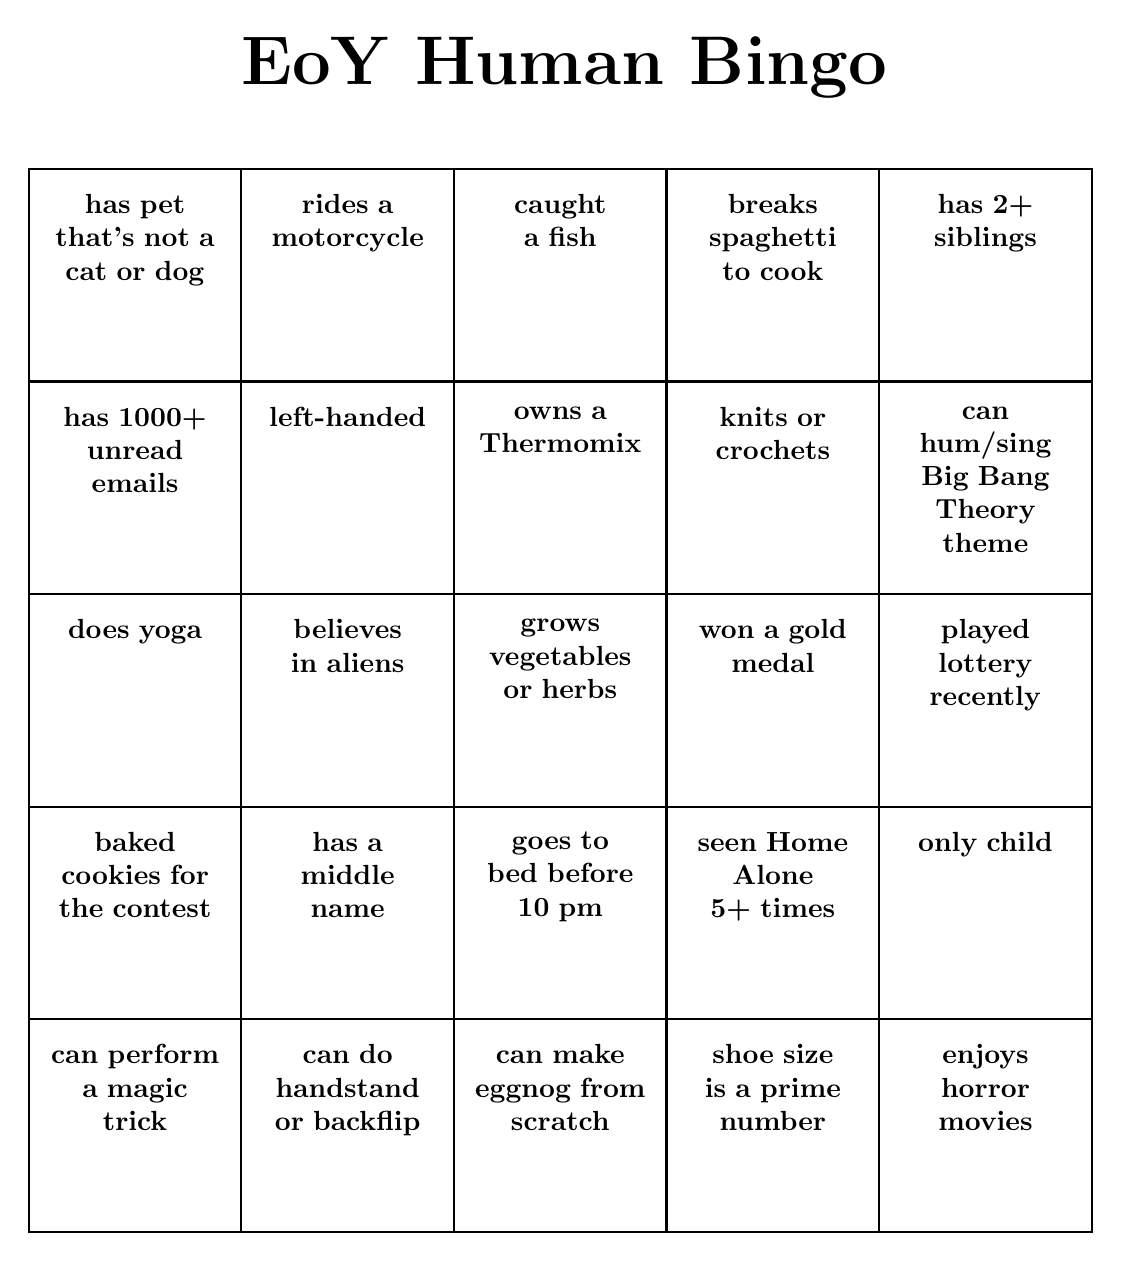
\begin{tikzpicture}
% Set the grid dimensions
\def\cellsize{2.7cm} % Each cell will be 2x2 cm

% Draw the grid and insert the numbers
\draw[thick] (0.0, 0.0) rectangle +(2.7, 2.7);
\node[anchor=north, align=center, text width=2.2cm] at (1.35, 2.5) {\textbf{has pet that's not a cat or dog}};
\draw[thick] (2.7, 0.0) rectangle +(2.7, 2.7);
\node[anchor=north, align=center, text width=2.2cm] at (4.050000000000001, 2.5) {\textbf{rides a motorcycle}};
\draw[thick] (5.4, 0.0) rectangle +(2.7, 2.7);
\node[anchor=north, align=center, text width=2.2cm] at (6.75, 2.5) {\textbf{caught a fish}};
\draw[thick] (8.100000000000001, 0.0) rectangle +(2.7, 2.7);
\node[anchor=north, align=center, text width=2.2cm] at (9.450000000000001, 2.5) {\textbf{breaks spaghetti to cook}};
\draw[thick] (10.8, 0.0) rectangle +(2.7, 2.7);
\node[anchor=north, align=center, text width=2.2cm] at (12.15, 2.5) {\textbf{has 2+ siblings}};
\draw[thick] (0.0, -2.7) rectangle +(2.7, 2.7);
\node[anchor=north, align=center, text width=2.2cm] at (1.35, -0.2) {\textbf{has 1000+ unread emails}};
\draw[thick] (2.7, -2.7) rectangle +(2.7, 2.7);
\node[anchor=north, align=center, text width=2.2cm] at (4.050000000000001, -0.2) {\textbf{left-handed}};
\draw[thick] (5.4, -2.7) rectangle +(2.7, 2.7);
\node[anchor=north, align=center, text width=2.2cm] at (6.75, -0.2) {\textbf{owns a Thermomix}};
\draw[thick] (8.100000000000001, -2.7) rectangle +(2.7, 2.7);
\node[anchor=north, align=center, text width=2.2cm] at (9.450000000000001, -0.2) {\textbf{knits or crochets}};
\draw[thick] (10.8, -2.7) rectangle +(2.7, 2.7);
\node[anchor=north, align=center, text width=2.2cm] at (12.15, -0.2) {\textbf{can hum/sing Big Bang Theory theme}};
\draw[thick] (0.0, -5.4) rectangle +(2.7, 2.7);
\node[anchor=north, align=center, text width=2.2cm] at (1.35, -2.9000000000000004) {\textbf{does yoga}};
\draw[thick] (2.7, -5.4) rectangle +(2.7, 2.7);
\node[anchor=north, align=center, text width=2.2cm] at (4.050000000000001, -2.9000000000000004) {\textbf{believes in aliens}};
\draw[thick] (5.4, -5.4) rectangle +(2.7, 2.7);
\node[anchor=north, align=center, text width=2.2cm] at (6.75, -2.9000000000000004) {\textbf{grows vegetables or herbs}};
\draw[thick] (8.100000000000001, -5.4) rectangle +(2.7, 2.7);
\node[anchor=north, align=center, text width=2.2cm] at (9.450000000000001, -2.9000000000000004) {\textbf{won a gold medal}};
\draw[thick] (10.8, -5.4) rectangle +(2.7, 2.7);
\node[anchor=north, align=center, text width=2.2cm] at (12.15, -2.9000000000000004) {\textbf{played lottery recently}};
\draw[thick] (0.0, -8.100000000000001) rectangle +(2.7, 2.7);
\node[anchor=north, align=center, text width=2.2cm] at (1.35, -5.600000000000001) {\textbf{baked cookies for the contest}};
\draw[thick] (2.7, -8.100000000000001) rectangle +(2.7, 2.7);
\node[anchor=north, align=center, text width=2.2cm] at (4.050000000000001, -5.600000000000001) {\textbf{has a middle name}};
\draw[thick] (5.4, -8.100000000000001) rectangle +(2.7, 2.7);
\node[anchor=north, align=center, text width=2.2cm] at (6.75, -5.600000000000001) {\textbf{goes to bed before 10 pm}};
\draw[thick] (8.100000000000001, -8.100000000000001) rectangle +(2.7, 2.7);
\node[anchor=north, align=center, text width=2.2cm] at (9.450000000000001, -5.600000000000001) {\textbf{seen Home Alone 5+ times}};
\draw[thick] (10.8, -8.100000000000001) rectangle +(2.7, 2.7);
\node[anchor=north, align=center, text width=2.2cm] at (12.15, -5.600000000000001) {\textbf{only child}};
\draw[thick] (0.0, -10.8) rectangle +(2.7, 2.7);
\node[anchor=north, align=center, text width=2.2cm] at (1.35, -8.3) {\textbf{can perform a magic trick}};
\draw[thick] (2.7, -10.8) rectangle +(2.7, 2.7);
\node[anchor=north, align=center, text width=2.2cm] at (4.050000000000001, -8.3) {\textbf{can do handstand or backflip}};
\draw[thick] (5.4, -10.8) rectangle +(2.7, 2.7);
\node[anchor=north, align=center, text width=2.2cm] at (6.75, -8.3) {\textbf{can make eggnog from scratch}};
\draw[thick] (8.100000000000001, -10.8) rectangle +(2.7, 2.7);
\node[anchor=north, align=center, text width=2.2cm] at (9.450000000000001, -8.3) {\textbf{shoe size is a prime number}};
\draw[thick] (10.8, -10.8) rectangle +(2.7, 2.7);
\node[anchor=north, align=center, text width=2.2cm] at (12.15, -8.3) {\textbf{enjoys horror movies}};
\node[anchor=north, font = \Huge] at (6.8, 4.5){\textbf{EoY Human Bingo}};
\end{tikzpicture}
\end{center}
\newpage\begin{center}
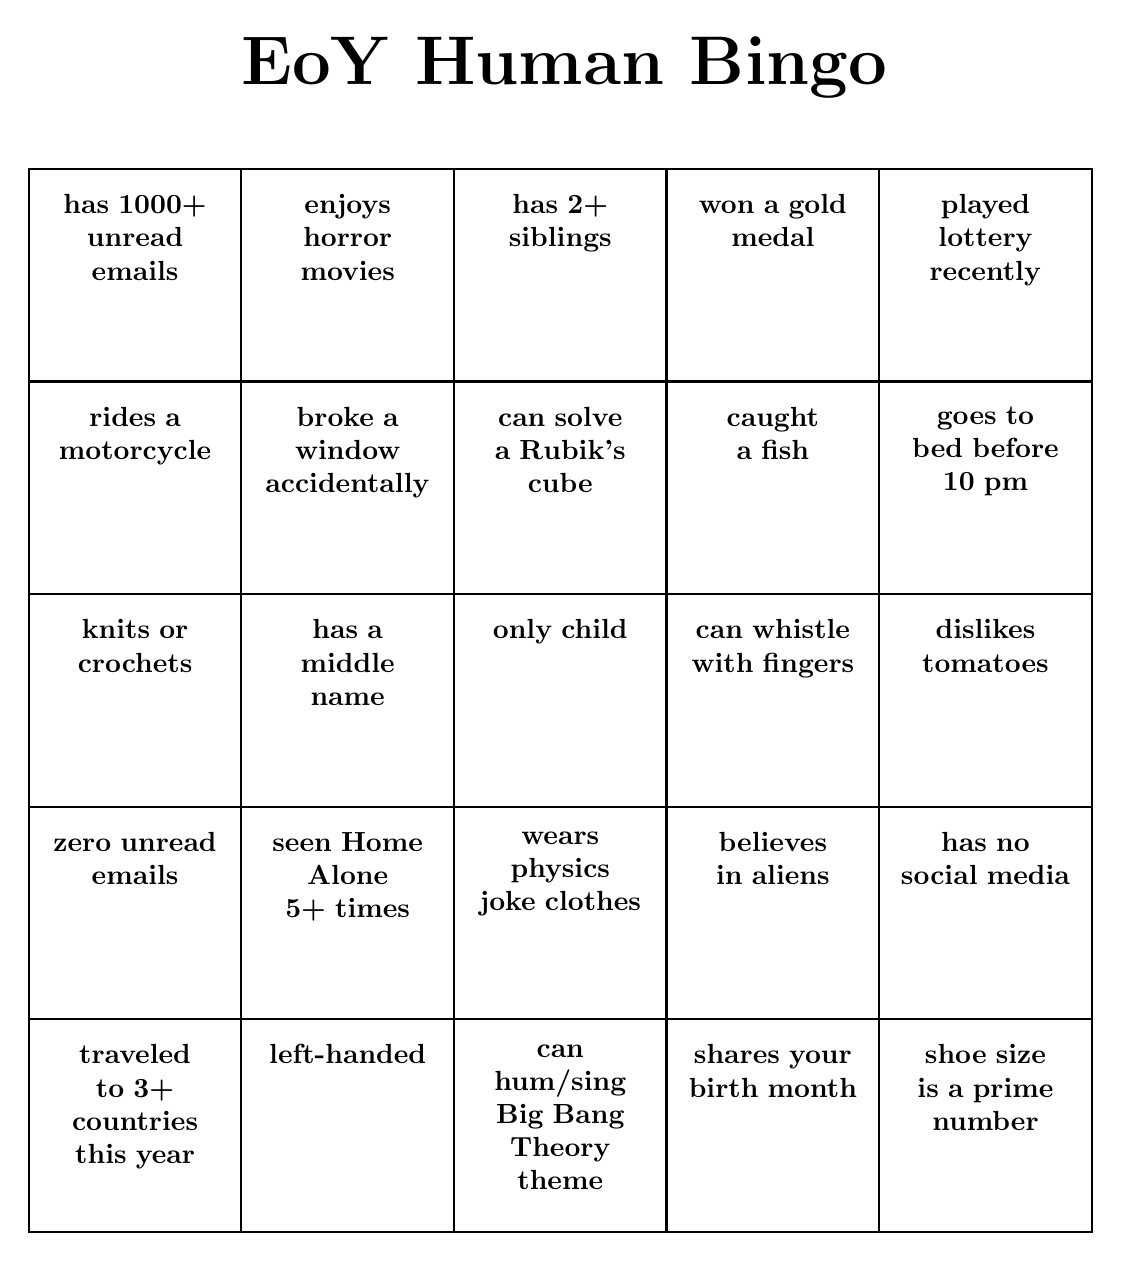
\begin{tikzpicture}
% Set the grid dimensions
\def\cellsize{2.7cm} % Each cell will be 2x2 cm

% Draw the grid and insert the numbers
\draw[thick] (0.0, 0.0) rectangle +(2.7, 2.7);
\node[anchor=north, align=center, text width=2.2cm] at (1.35, 2.5) {\textbf{has 1000+ unread emails}};
\draw[thick] (2.7, 0.0) rectangle +(2.7, 2.7);
\node[anchor=north, align=center, text width=2.2cm] at (4.050000000000001, 2.5) {\textbf{enjoys horror movies}};
\draw[thick] (5.4, 0.0) rectangle +(2.7, 2.7);
\node[anchor=north, align=center, text width=2.2cm] at (6.75, 2.5) {\textbf{has 2+ siblings}};
\draw[thick] (8.100000000000001, 0.0) rectangle +(2.7, 2.7);
\node[anchor=north, align=center, text width=2.2cm] at (9.450000000000001, 2.5) {\textbf{won a gold medal}};
\draw[thick] (10.8, 0.0) rectangle +(2.7, 2.7);
\node[anchor=north, align=center, text width=2.2cm] at (12.15, 2.5) {\textbf{played lottery recently}};
\draw[thick] (0.0, -2.7) rectangle +(2.7, 2.7);
\node[anchor=north, align=center, text width=2.2cm] at (1.35, -0.2) {\textbf{rides a motorcycle}};
\draw[thick] (2.7, -2.7) rectangle +(2.7, 2.7);
\node[anchor=north, align=center, text width=2.2cm] at (4.050000000000001, -0.2) {\textbf{broke a window accidentally}};
\draw[thick] (5.4, -2.7) rectangle +(2.7, 2.7);
\node[anchor=north, align=center, text width=2.2cm] at (6.75, -0.2) {\textbf{can solve a Rubik's cube}};
\draw[thick] (8.100000000000001, -2.7) rectangle +(2.7, 2.7);
\node[anchor=north, align=center, text width=2.2cm] at (9.450000000000001, -0.2) {\textbf{caught a fish}};
\draw[thick] (10.8, -2.7) rectangle +(2.7, 2.7);
\node[anchor=north, align=center, text width=2.2cm] at (12.15, -0.2) {\textbf{goes to bed before 10 pm}};
\draw[thick] (0.0, -5.4) rectangle +(2.7, 2.7);
\node[anchor=north, align=center, text width=2.2cm] at (1.35, -2.9000000000000004) {\textbf{knits or crochets}};
\draw[thick] (2.7, -5.4) rectangle +(2.7, 2.7);
\node[anchor=north, align=center, text width=2.2cm] at (4.050000000000001, -2.9000000000000004) {\textbf{has a middle name}};
\draw[thick] (5.4, -5.4) rectangle +(2.7, 2.7);
\node[anchor=north, align=center, text width=2.2cm] at (6.75, -2.9000000000000004) {\textbf{only child}};
\draw[thick] (8.100000000000001, -5.4) rectangle +(2.7, 2.7);
\node[anchor=north, align=center, text width=2.2cm] at (9.450000000000001, -2.9000000000000004) {\textbf{can whistle with fingers}};
\draw[thick] (10.8, -5.4) rectangle +(2.7, 2.7);
\node[anchor=north, align=center, text width=2.2cm] at (12.15, -2.9000000000000004) {\textbf{dislikes tomatoes}};
\draw[thick] (0.0, -8.100000000000001) rectangle +(2.7, 2.7);
\node[anchor=north, align=center, text width=2.2cm] at (1.35, -5.600000000000001) {\textbf{zero unread emails}};
\draw[thick] (2.7, -8.100000000000001) rectangle +(2.7, 2.7);
\node[anchor=north, align=center, text width=2.2cm] at (4.050000000000001, -5.600000000000001) {\textbf{seen Home Alone 5+ times}};
\draw[thick] (5.4, -8.100000000000001) rectangle +(2.7, 2.7);
\node[anchor=north, align=center, text width=2.2cm] at (6.75, -5.600000000000001) {\textbf{wears physics joke clothes}};
\draw[thick] (8.100000000000001, -8.100000000000001) rectangle +(2.7, 2.7);
\node[anchor=north, align=center, text width=2.2cm] at (9.450000000000001, -5.600000000000001) {\textbf{believes in aliens}};
\draw[thick] (10.8, -8.100000000000001) rectangle +(2.7, 2.7);
\node[anchor=north, align=center, text width=2.2cm] at (12.15, -5.600000000000001) {\textbf{has no social media}};
\draw[thick] (0.0, -10.8) rectangle +(2.7, 2.7);
\node[anchor=north, align=center, text width=2.2cm] at (1.35, -8.3) {\textbf{traveled to 3+ countries this year}};
\draw[thick] (2.7, -10.8) rectangle +(2.7, 2.7);
\node[anchor=north, align=center, text width=2.2cm] at (4.050000000000001, -8.3) {\textbf{left-handed}};
\draw[thick] (5.4, -10.8) rectangle +(2.7, 2.7);
\node[anchor=north, align=center, text width=2.2cm] at (6.75, -8.3) {\textbf{can hum/sing Big Bang Theory theme}};
\draw[thick] (8.100000000000001, -10.8) rectangle +(2.7, 2.7);
\node[anchor=north, align=center, text width=2.2cm] at (9.450000000000001, -8.3) {\textbf{shares your birth month}};
\draw[thick] (10.8, -10.8) rectangle +(2.7, 2.7);
\node[anchor=north, align=center, text width=2.2cm] at (12.15, -8.3) {\textbf{shoe size is a prime number}};
\node[anchor=north, font = \Huge] at (6.8, 4.5){\textbf{EoY Human Bingo}};
\end{tikzpicture}
\end{center}
\newpage\begin{center}
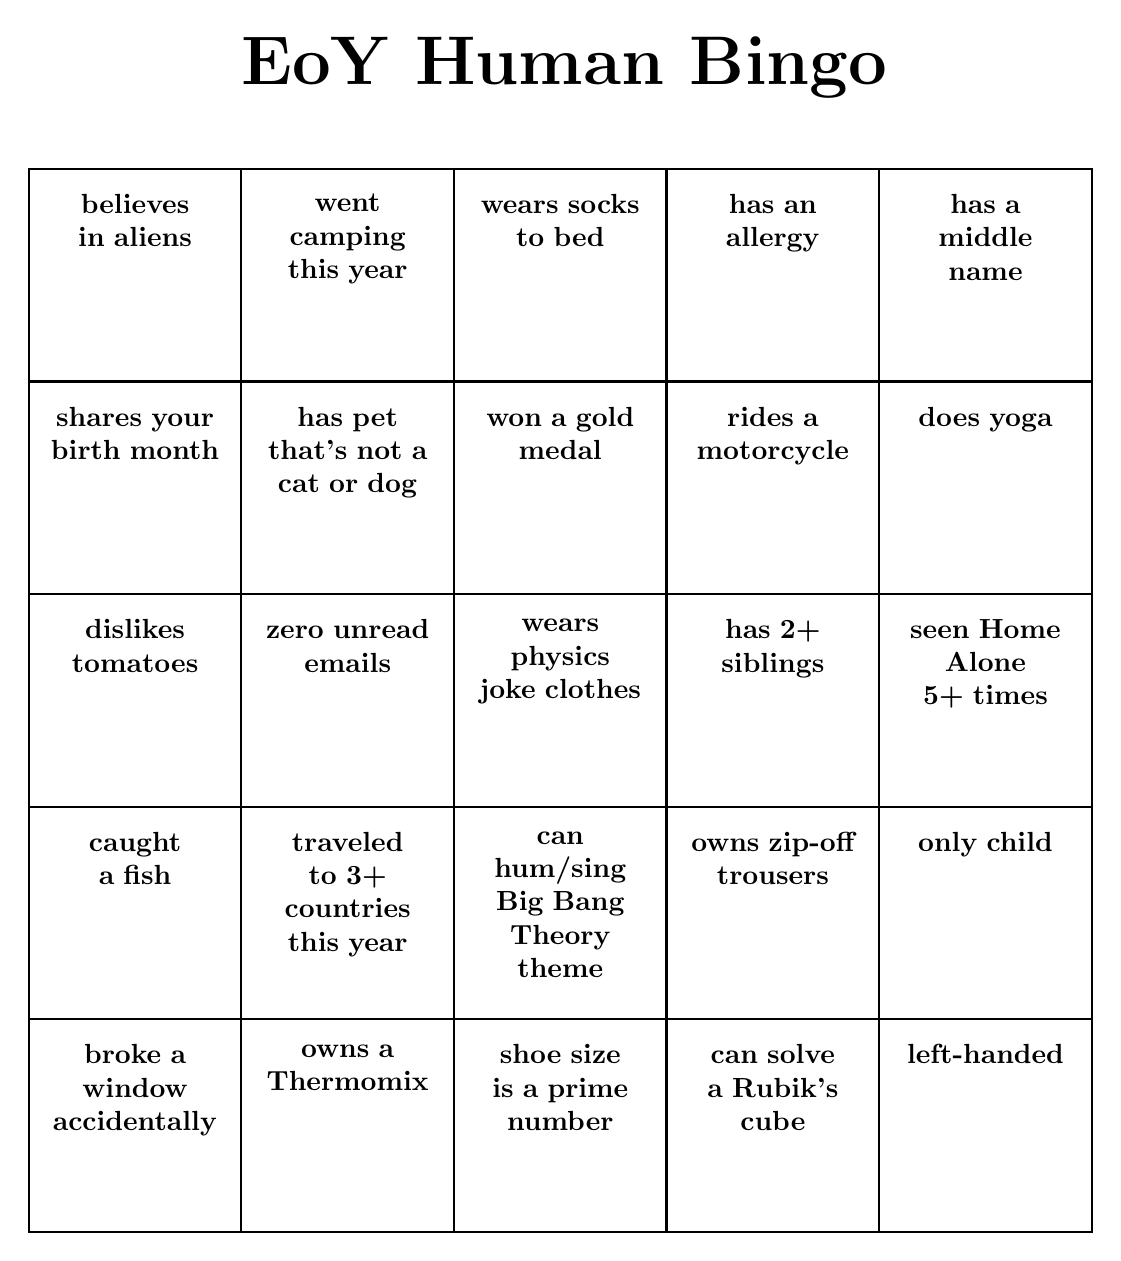
\begin{tikzpicture}
% Set the grid dimensions
\def\cellsize{2.7cm} % Each cell will be 2x2 cm

% Draw the grid and insert the numbers
\draw[thick] (0.0, 0.0) rectangle +(2.7, 2.7);
\node[anchor=north, align=center, text width=2.2cm] at (1.35, 2.5) {\textbf{believes in aliens}};
\draw[thick] (2.7, 0.0) rectangle +(2.7, 2.7);
\node[anchor=north, align=center, text width=2.2cm] at (4.050000000000001, 2.5) {\textbf{went camping this year}};
\draw[thick] (5.4, 0.0) rectangle +(2.7, 2.7);
\node[anchor=north, align=center, text width=2.2cm] at (6.75, 2.5) {\textbf{wears socks to bed}};
\draw[thick] (8.100000000000001, 0.0) rectangle +(2.7, 2.7);
\node[anchor=north, align=center, text width=2.2cm] at (9.450000000000001, 2.5) {\textbf{has an allergy}};
\draw[thick] (10.8, 0.0) rectangle +(2.7, 2.7);
\node[anchor=north, align=center, text width=2.2cm] at (12.15, 2.5) {\textbf{has a middle name}};
\draw[thick] (0.0, -2.7) rectangle +(2.7, 2.7);
\node[anchor=north, align=center, text width=2.2cm] at (1.35, -0.2) {\textbf{shares your birth month}};
\draw[thick] (2.7, -2.7) rectangle +(2.7, 2.7);
\node[anchor=north, align=center, text width=2.2cm] at (4.050000000000001, -0.2) {\textbf{has pet that's not a cat or dog}};
\draw[thick] (5.4, -2.7) rectangle +(2.7, 2.7);
\node[anchor=north, align=center, text width=2.2cm] at (6.75, -0.2) {\textbf{won a gold medal}};
\draw[thick] (8.100000000000001, -2.7) rectangle +(2.7, 2.7);
\node[anchor=north, align=center, text width=2.2cm] at (9.450000000000001, -0.2) {\textbf{rides a motorcycle}};
\draw[thick] (10.8, -2.7) rectangle +(2.7, 2.7);
\node[anchor=north, align=center, text width=2.2cm] at (12.15, -0.2) {\textbf{does yoga}};
\draw[thick] (0.0, -5.4) rectangle +(2.7, 2.7);
\node[anchor=north, align=center, text width=2.2cm] at (1.35, -2.9000000000000004) {\textbf{dislikes tomatoes}};
\draw[thick] (2.7, -5.4) rectangle +(2.7, 2.7);
\node[anchor=north, align=center, text width=2.2cm] at (4.050000000000001, -2.9000000000000004) {\textbf{zero unread emails}};
\draw[thick] (5.4, -5.4) rectangle +(2.7, 2.7);
\node[anchor=north, align=center, text width=2.2cm] at (6.75, -2.9000000000000004) {\textbf{wears physics joke clothes}};
\draw[thick] (8.100000000000001, -5.4) rectangle +(2.7, 2.7);
\node[anchor=north, align=center, text width=2.2cm] at (9.450000000000001, -2.9000000000000004) {\textbf{has 2+ siblings}};
\draw[thick] (10.8, -5.4) rectangle +(2.7, 2.7);
\node[anchor=north, align=center, text width=2.2cm] at (12.15, -2.9000000000000004) {\textbf{seen Home Alone 5+ times}};
\draw[thick] (0.0, -8.100000000000001) rectangle +(2.7, 2.7);
\node[anchor=north, align=center, text width=2.2cm] at (1.35, -5.600000000000001) {\textbf{caught a fish}};
\draw[thick] (2.7, -8.100000000000001) rectangle +(2.7, 2.7);
\node[anchor=north, align=center, text width=2.2cm] at (4.050000000000001, -5.600000000000001) {\textbf{traveled to 3+ countries this year}};
\draw[thick] (5.4, -8.100000000000001) rectangle +(2.7, 2.7);
\node[anchor=north, align=center, text width=2.2cm] at (6.75, -5.600000000000001) {\textbf{can hum/sing Big Bang Theory theme}};
\draw[thick] (8.100000000000001, -8.100000000000001) rectangle +(2.7, 2.7);
\node[anchor=north, align=center, text width=2.2cm] at (9.450000000000001, -5.600000000000001) {\textbf{owns zip-off trousers}};
\draw[thick] (10.8, -8.100000000000001) rectangle +(2.7, 2.7);
\node[anchor=north, align=center, text width=2.2cm] at (12.15, -5.600000000000001) {\textbf{only child}};
\draw[thick] (0.0, -10.8) rectangle +(2.7, 2.7);
\node[anchor=north, align=center, text width=2.2cm] at (1.35, -8.3) {\textbf{broke a window accidentally}};
\draw[thick] (2.7, -10.8) rectangle +(2.7, 2.7);
\node[anchor=north, align=center, text width=2.2cm] at (4.050000000000001, -8.3) {\textbf{owns a Thermomix}};
\draw[thick] (5.4, -10.8) rectangle +(2.7, 2.7);
\node[anchor=north, align=center, text width=2.2cm] at (6.75, -8.3) {\textbf{shoe size is a prime number}};
\draw[thick] (8.100000000000001, -10.8) rectangle +(2.7, 2.7);
\node[anchor=north, align=center, text width=2.2cm] at (9.450000000000001, -8.3) {\textbf{can solve a Rubik's cube}};
\draw[thick] (10.8, -10.8) rectangle +(2.7, 2.7);
\node[anchor=north, align=center, text width=2.2cm] at (12.15, -8.3) {\textbf{left-handed}};
\node[anchor=north, font = \Huge] at (6.8, 4.5){\textbf{EoY Human Bingo}};
\end{tikzpicture}
\end{center}
\newpage\begin{center}
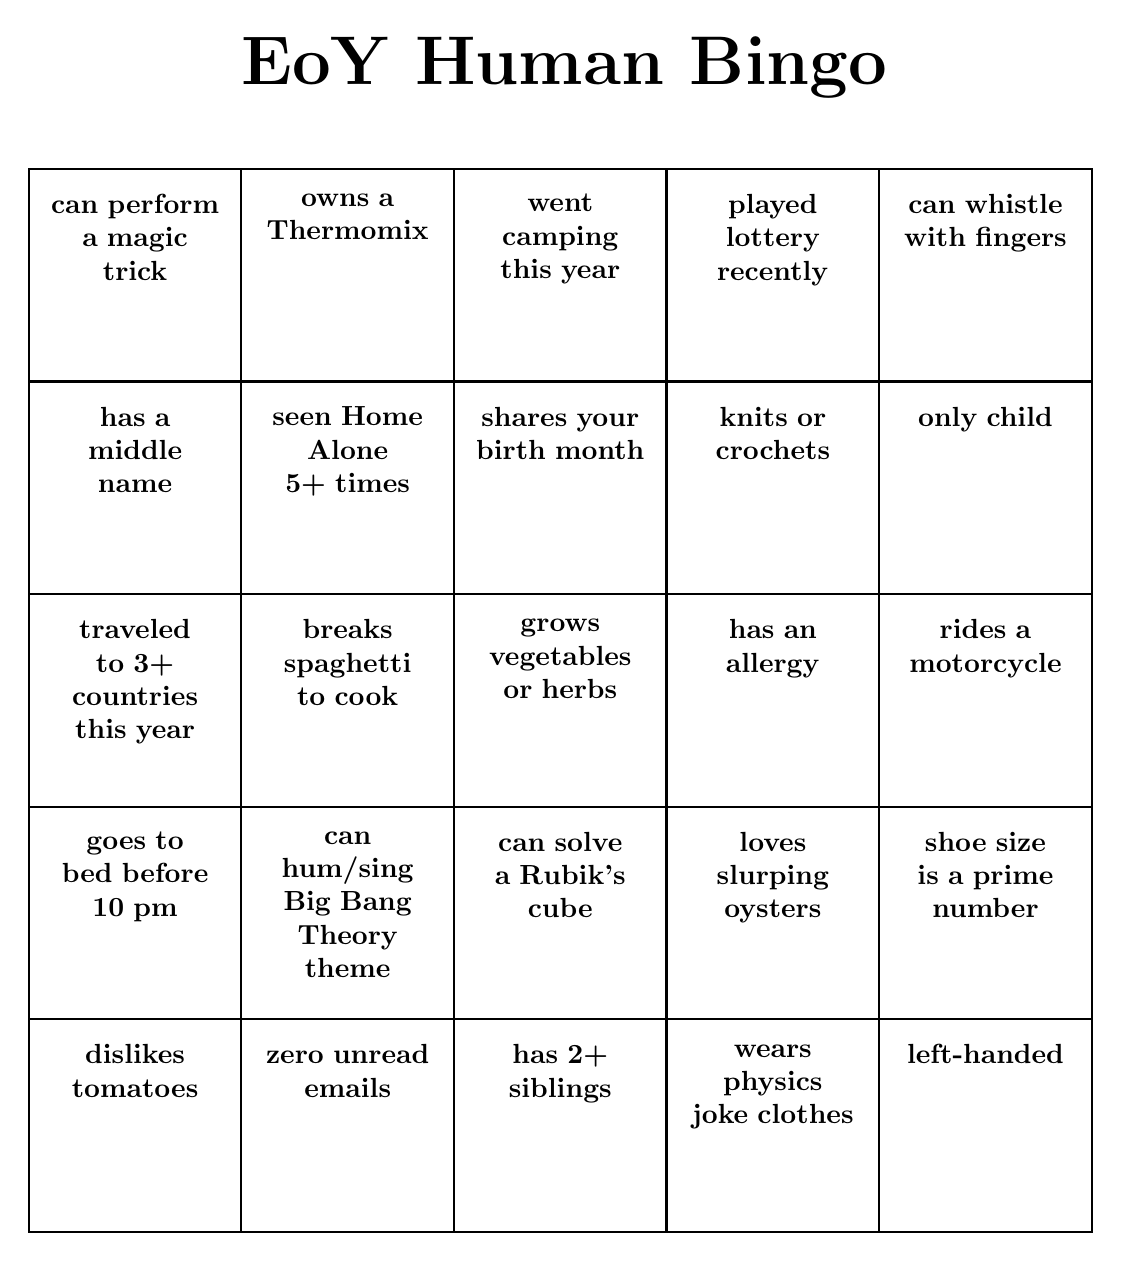
\begin{tikzpicture}
% Set the grid dimensions
\def\cellsize{2.7cm} % Each cell will be 2x2 cm

% Draw the grid and insert the numbers
\draw[thick] (0.0, 0.0) rectangle +(2.7, 2.7);
\node[anchor=north, align=center, text width=2.2cm] at (1.35, 2.5) {\textbf{can perform a magic trick}};
\draw[thick] (2.7, 0.0) rectangle +(2.7, 2.7);
\node[anchor=north, align=center, text width=2.2cm] at (4.050000000000001, 2.5) {\textbf{owns a Thermomix}};
\draw[thick] (5.4, 0.0) rectangle +(2.7, 2.7);
\node[anchor=north, align=center, text width=2.2cm] at (6.75, 2.5) {\textbf{went camping this year}};
\draw[thick] (8.100000000000001, 0.0) rectangle +(2.7, 2.7);
\node[anchor=north, align=center, text width=2.2cm] at (9.450000000000001, 2.5) {\textbf{played lottery recently}};
\draw[thick] (10.8, 0.0) rectangle +(2.7, 2.7);
\node[anchor=north, align=center, text width=2.2cm] at (12.15, 2.5) {\textbf{can whistle with fingers}};
\draw[thick] (0.0, -2.7) rectangle +(2.7, 2.7);
\node[anchor=north, align=center, text width=2.2cm] at (1.35, -0.2) {\textbf{has a middle name}};
\draw[thick] (2.7, -2.7) rectangle +(2.7, 2.7);
\node[anchor=north, align=center, text width=2.2cm] at (4.050000000000001, -0.2) {\textbf{seen Home Alone 5+ times}};
\draw[thick] (5.4, -2.7) rectangle +(2.7, 2.7);
\node[anchor=north, align=center, text width=2.2cm] at (6.75, -0.2) {\textbf{shares your birth month}};
\draw[thick] (8.100000000000001, -2.7) rectangle +(2.7, 2.7);
\node[anchor=north, align=center, text width=2.2cm] at (9.450000000000001, -0.2) {\textbf{knits or crochets}};
\draw[thick] (10.8, -2.7) rectangle +(2.7, 2.7);
\node[anchor=north, align=center, text width=2.2cm] at (12.15, -0.2) {\textbf{only child}};
\draw[thick] (0.0, -5.4) rectangle +(2.7, 2.7);
\node[anchor=north, align=center, text width=2.2cm] at (1.35, -2.9000000000000004) {\textbf{traveled to 3+ countries this year}};
\draw[thick] (2.7, -5.4) rectangle +(2.7, 2.7);
\node[anchor=north, align=center, text width=2.2cm] at (4.050000000000001, -2.9000000000000004) {\textbf{breaks spaghetti to cook}};
\draw[thick] (5.4, -5.4) rectangle +(2.7, 2.7);
\node[anchor=north, align=center, text width=2.2cm] at (6.75, -2.9000000000000004) {\textbf{grows vegetables or herbs}};
\draw[thick] (8.100000000000001, -5.4) rectangle +(2.7, 2.7);
\node[anchor=north, align=center, text width=2.2cm] at (9.450000000000001, -2.9000000000000004) {\textbf{has an allergy}};
\draw[thick] (10.8, -5.4) rectangle +(2.7, 2.7);
\node[anchor=north, align=center, text width=2.2cm] at (12.15, -2.9000000000000004) {\textbf{rides a motorcycle}};
\draw[thick] (0.0, -8.100000000000001) rectangle +(2.7, 2.7);
\node[anchor=north, align=center, text width=2.2cm] at (1.35, -5.600000000000001) {\textbf{goes to bed before 10 pm}};
\draw[thick] (2.7, -8.100000000000001) rectangle +(2.7, 2.7);
\node[anchor=north, align=center, text width=2.2cm] at (4.050000000000001, -5.600000000000001) {\textbf{can hum/sing Big Bang Theory theme}};
\draw[thick] (5.4, -8.100000000000001) rectangle +(2.7, 2.7);
\node[anchor=north, align=center, text width=2.2cm] at (6.75, -5.600000000000001) {\textbf{can solve a Rubik's cube}};
\draw[thick] (8.100000000000001, -8.100000000000001) rectangle +(2.7, 2.7);
\node[anchor=north, align=center, text width=2.2cm] at (9.450000000000001, -5.600000000000001) {\textbf{loves slurping oysters}};
\draw[thick] (10.8, -8.100000000000001) rectangle +(2.7, 2.7);
\node[anchor=north, align=center, text width=2.2cm] at (12.15, -5.600000000000001) {\textbf{shoe size is a prime number}};
\draw[thick] (0.0, -10.8) rectangle +(2.7, 2.7);
\node[anchor=north, align=center, text width=2.2cm] at (1.35, -8.3) {\textbf{dislikes tomatoes}};
\draw[thick] (2.7, -10.8) rectangle +(2.7, 2.7);
\node[anchor=north, align=center, text width=2.2cm] at (4.050000000000001, -8.3) {\textbf{zero unread emails}};
\draw[thick] (5.4, -10.8) rectangle +(2.7, 2.7);
\node[anchor=north, align=center, text width=2.2cm] at (6.75, -8.3) {\textbf{has 2+ siblings}};
\draw[thick] (8.100000000000001, -10.8) rectangle +(2.7, 2.7);
\node[anchor=north, align=center, text width=2.2cm] at (9.450000000000001, -8.3) {\textbf{wears physics joke clothes}};
\draw[thick] (10.8, -10.8) rectangle +(2.7, 2.7);
\node[anchor=north, align=center, text width=2.2cm] at (12.15, -8.3) {\textbf{left-handed}};
\node[anchor=north, font = \Huge] at (6.8, 4.5){\textbf{EoY Human Bingo}};
\end{tikzpicture}
\end{center}
\newpage\begin{center}
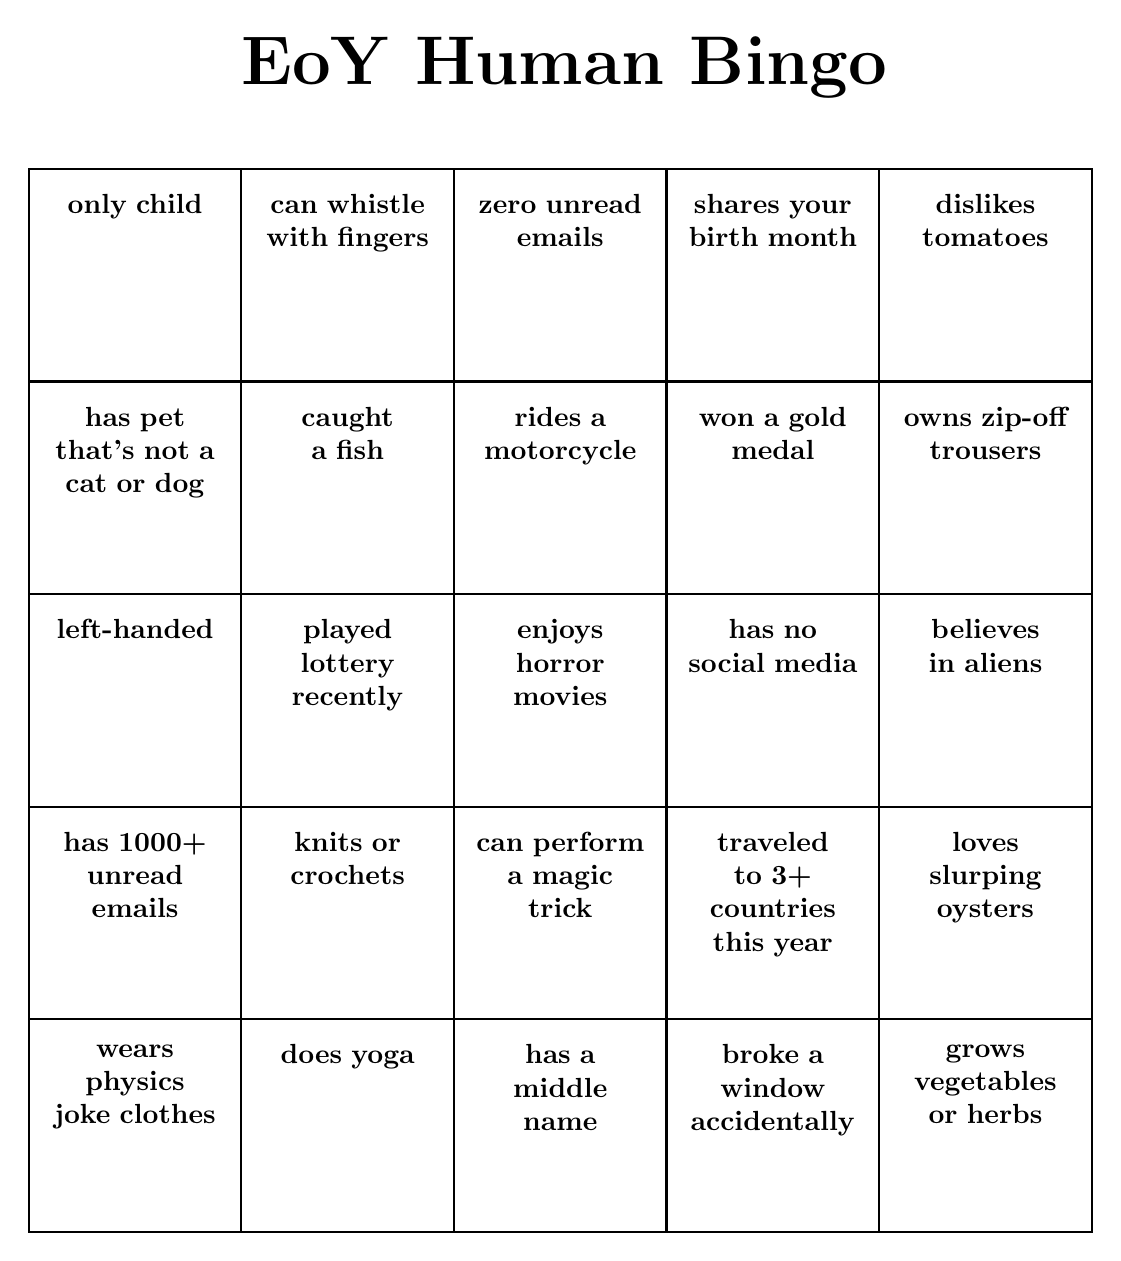
\begin{tikzpicture}
% Set the grid dimensions
\def\cellsize{2.7cm} % Each cell will be 2x2 cm

% Draw the grid and insert the numbers
\draw[thick] (0.0, 0.0) rectangle +(2.7, 2.7);
\node[anchor=north, align=center, text width=2.2cm] at (1.35, 2.5) {\textbf{only child}};
\draw[thick] (2.7, 0.0) rectangle +(2.7, 2.7);
\node[anchor=north, align=center, text width=2.2cm] at (4.050000000000001, 2.5) {\textbf{can whistle with fingers}};
\draw[thick] (5.4, 0.0) rectangle +(2.7, 2.7);
\node[anchor=north, align=center, text width=2.2cm] at (6.75, 2.5) {\textbf{zero unread emails}};
\draw[thick] (8.100000000000001, 0.0) rectangle +(2.7, 2.7);
\node[anchor=north, align=center, text width=2.2cm] at (9.450000000000001, 2.5) {\textbf{shares your birth month}};
\draw[thick] (10.8, 0.0) rectangle +(2.7, 2.7);
\node[anchor=north, align=center, text width=2.2cm] at (12.15, 2.5) {\textbf{dislikes tomatoes}};
\draw[thick] (0.0, -2.7) rectangle +(2.7, 2.7);
\node[anchor=north, align=center, text width=2.2cm] at (1.35, -0.2) {\textbf{has pet that's not a cat or dog}};
\draw[thick] (2.7, -2.7) rectangle +(2.7, 2.7);
\node[anchor=north, align=center, text width=2.2cm] at (4.050000000000001, -0.2) {\textbf{caught a fish}};
\draw[thick] (5.4, -2.7) rectangle +(2.7, 2.7);
\node[anchor=north, align=center, text width=2.2cm] at (6.75, -0.2) {\textbf{rides a motorcycle}};
\draw[thick] (8.100000000000001, -2.7) rectangle +(2.7, 2.7);
\node[anchor=north, align=center, text width=2.2cm] at (9.450000000000001, -0.2) {\textbf{won a gold medal}};
\draw[thick] (10.8, -2.7) rectangle +(2.7, 2.7);
\node[anchor=north, align=center, text width=2.2cm] at (12.15, -0.2) {\textbf{owns zip-off trousers}};
\draw[thick] (0.0, -5.4) rectangle +(2.7, 2.7);
\node[anchor=north, align=center, text width=2.2cm] at (1.35, -2.9000000000000004) {\textbf{left-handed}};
\draw[thick] (2.7, -5.4) rectangle +(2.7, 2.7);
\node[anchor=north, align=center, text width=2.2cm] at (4.050000000000001, -2.9000000000000004) {\textbf{played lottery recently}};
\draw[thick] (5.4, -5.4) rectangle +(2.7, 2.7);
\node[anchor=north, align=center, text width=2.2cm] at (6.75, -2.9000000000000004) {\textbf{enjoys horror movies}};
\draw[thick] (8.100000000000001, -5.4) rectangle +(2.7, 2.7);
\node[anchor=north, align=center, text width=2.2cm] at (9.450000000000001, -2.9000000000000004) {\textbf{has no social media}};
\draw[thick] (10.8, -5.4) rectangle +(2.7, 2.7);
\node[anchor=north, align=center, text width=2.2cm] at (12.15, -2.9000000000000004) {\textbf{believes in aliens}};
\draw[thick] (0.0, -8.100000000000001) rectangle +(2.7, 2.7);
\node[anchor=north, align=center, text width=2.2cm] at (1.35, -5.600000000000001) {\textbf{has 1000+ unread emails}};
\draw[thick] (2.7, -8.100000000000001) rectangle +(2.7, 2.7);
\node[anchor=north, align=center, text width=2.2cm] at (4.050000000000001, -5.600000000000001) {\textbf{knits or crochets}};
\draw[thick] (5.4, -8.100000000000001) rectangle +(2.7, 2.7);
\node[anchor=north, align=center, text width=2.2cm] at (6.75, -5.600000000000001) {\textbf{can perform a magic trick}};
\draw[thick] (8.100000000000001, -8.100000000000001) rectangle +(2.7, 2.7);
\node[anchor=north, align=center, text width=2.2cm] at (9.450000000000001, -5.600000000000001) {\textbf{traveled to 3+ countries this year}};
\draw[thick] (10.8, -8.100000000000001) rectangle +(2.7, 2.7);
\node[anchor=north, align=center, text width=2.2cm] at (12.15, -5.600000000000001) {\textbf{loves slurping oysters}};
\draw[thick] (0.0, -10.8) rectangle +(2.7, 2.7);
\node[anchor=north, align=center, text width=2.2cm] at (1.35, -8.3) {\textbf{wears physics joke clothes}};
\draw[thick] (2.7, -10.8) rectangle +(2.7, 2.7);
\node[anchor=north, align=center, text width=2.2cm] at (4.050000000000001, -8.3) {\textbf{does yoga}};
\draw[thick] (5.4, -10.8) rectangle +(2.7, 2.7);
\node[anchor=north, align=center, text width=2.2cm] at (6.75, -8.3) {\textbf{has a middle name}};
\draw[thick] (8.100000000000001, -10.8) rectangle +(2.7, 2.7);
\node[anchor=north, align=center, text width=2.2cm] at (9.450000000000001, -8.3) {\textbf{broke a window accidentally}};
\draw[thick] (10.8, -10.8) rectangle +(2.7, 2.7);
\node[anchor=north, align=center, text width=2.2cm] at (12.15, -8.3) {\textbf{grows vegetables or herbs}};
\node[anchor=north, font = \Huge] at (6.8, 4.5){\textbf{EoY Human Bingo}};
\end{tikzpicture}
\end{center}
\newpage\begin{center}
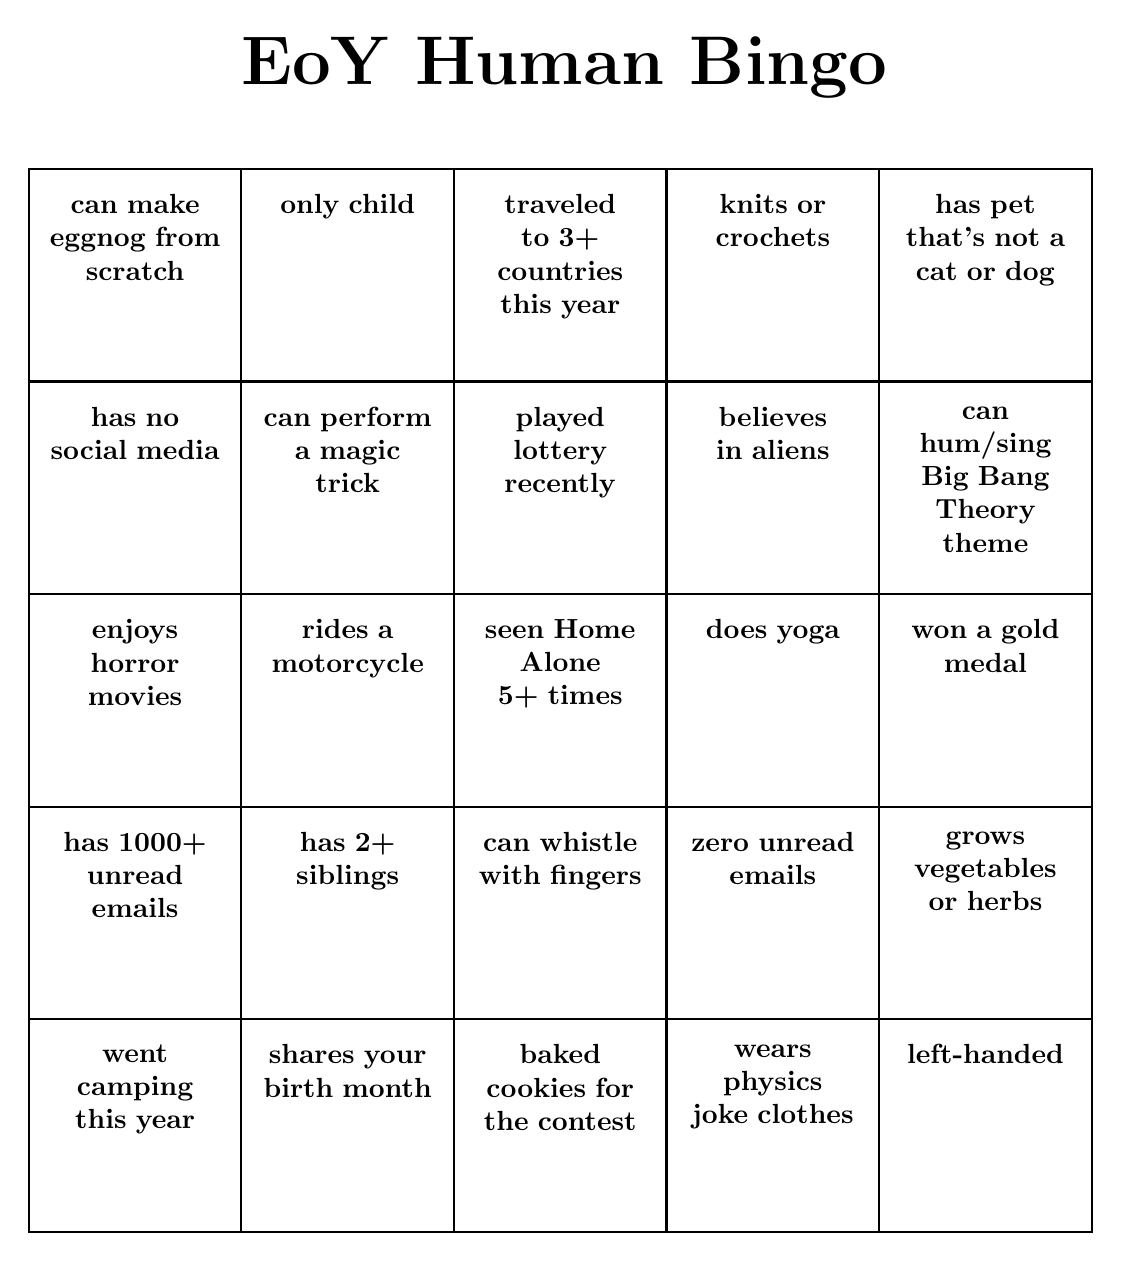
\begin{tikzpicture}
% Set the grid dimensions
\def\cellsize{2.7cm} % Each cell will be 2x2 cm

% Draw the grid and insert the numbers
\draw[thick] (0.0, 0.0) rectangle +(2.7, 2.7);
\node[anchor=north, align=center, text width=2.2cm] at (1.35, 2.5) {\textbf{can make eggnog from scratch}};
\draw[thick] (2.7, 0.0) rectangle +(2.7, 2.7);
\node[anchor=north, align=center, text width=2.2cm] at (4.050000000000001, 2.5) {\textbf{only child}};
\draw[thick] (5.4, 0.0) rectangle +(2.7, 2.7);
\node[anchor=north, align=center, text width=2.2cm] at (6.75, 2.5) {\textbf{traveled to 3+ countries this year}};
\draw[thick] (8.100000000000001, 0.0) rectangle +(2.7, 2.7);
\node[anchor=north, align=center, text width=2.2cm] at (9.450000000000001, 2.5) {\textbf{knits or crochets}};
\draw[thick] (10.8, 0.0) rectangle +(2.7, 2.7);
\node[anchor=north, align=center, text width=2.2cm] at (12.15, 2.5) {\textbf{has pet that's not a cat or dog}};
\draw[thick] (0.0, -2.7) rectangle +(2.7, 2.7);
\node[anchor=north, align=center, text width=2.2cm] at (1.35, -0.2) {\textbf{has no social media}};
\draw[thick] (2.7, -2.7) rectangle +(2.7, 2.7);
\node[anchor=north, align=center, text width=2.2cm] at (4.050000000000001, -0.2) {\textbf{can perform a magic trick}};
\draw[thick] (5.4, -2.7) rectangle +(2.7, 2.7);
\node[anchor=north, align=center, text width=2.2cm] at (6.75, -0.2) {\textbf{played lottery recently}};
\draw[thick] (8.100000000000001, -2.7) rectangle +(2.7, 2.7);
\node[anchor=north, align=center, text width=2.2cm] at (9.450000000000001, -0.2) {\textbf{believes in aliens}};
\draw[thick] (10.8, -2.7) rectangle +(2.7, 2.7);
\node[anchor=north, align=center, text width=2.2cm] at (12.15, -0.2) {\textbf{can hum/sing Big Bang Theory theme}};
\draw[thick] (0.0, -5.4) rectangle +(2.7, 2.7);
\node[anchor=north, align=center, text width=2.2cm] at (1.35, -2.9000000000000004) {\textbf{enjoys horror movies}};
\draw[thick] (2.7, -5.4) rectangle +(2.7, 2.7);
\node[anchor=north, align=center, text width=2.2cm] at (4.050000000000001, -2.9000000000000004) {\textbf{rides a motorcycle}};
\draw[thick] (5.4, -5.4) rectangle +(2.7, 2.7);
\node[anchor=north, align=center, text width=2.2cm] at (6.75, -2.9000000000000004) {\textbf{seen Home Alone 5+ times}};
\draw[thick] (8.100000000000001, -5.4) rectangle +(2.7, 2.7);
\node[anchor=north, align=center, text width=2.2cm] at (9.450000000000001, -2.9000000000000004) {\textbf{does yoga}};
\draw[thick] (10.8, -5.4) rectangle +(2.7, 2.7);
\node[anchor=north, align=center, text width=2.2cm] at (12.15, -2.9000000000000004) {\textbf{won a gold medal}};
\draw[thick] (0.0, -8.100000000000001) rectangle +(2.7, 2.7);
\node[anchor=north, align=center, text width=2.2cm] at (1.35, -5.600000000000001) {\textbf{has 1000+ unread emails}};
\draw[thick] (2.7, -8.100000000000001) rectangle +(2.7, 2.7);
\node[anchor=north, align=center, text width=2.2cm] at (4.050000000000001, -5.600000000000001) {\textbf{has 2+ siblings}};
\draw[thick] (5.4, -8.100000000000001) rectangle +(2.7, 2.7);
\node[anchor=north, align=center, text width=2.2cm] at (6.75, -5.600000000000001) {\textbf{can whistle with fingers}};
\draw[thick] (8.100000000000001, -8.100000000000001) rectangle +(2.7, 2.7);
\node[anchor=north, align=center, text width=2.2cm] at (9.450000000000001, -5.600000000000001) {\textbf{zero unread emails}};
\draw[thick] (10.8, -8.100000000000001) rectangle +(2.7, 2.7);
\node[anchor=north, align=center, text width=2.2cm] at (12.15, -5.600000000000001) {\textbf{grows vegetables or herbs}};
\draw[thick] (0.0, -10.8) rectangle +(2.7, 2.7);
\node[anchor=north, align=center, text width=2.2cm] at (1.35, -8.3) {\textbf{went camping this year}};
\draw[thick] (2.7, -10.8) rectangle +(2.7, 2.7);
\node[anchor=north, align=center, text width=2.2cm] at (4.050000000000001, -8.3) {\textbf{shares your birth month}};
\draw[thick] (5.4, -10.8) rectangle +(2.7, 2.7);
\node[anchor=north, align=center, text width=2.2cm] at (6.75, -8.3) {\textbf{baked cookies for the contest}};
\draw[thick] (8.100000000000001, -10.8) rectangle +(2.7, 2.7);
\node[anchor=north, align=center, text width=2.2cm] at (9.450000000000001, -8.3) {\textbf{wears physics joke clothes}};
\draw[thick] (10.8, -10.8) rectangle +(2.7, 2.7);
\node[anchor=north, align=center, text width=2.2cm] at (12.15, -8.3) {\textbf{left-handed}};
\node[anchor=north, font = \Huge] at (6.8, 4.5){\textbf{EoY Human Bingo}};
\end{tikzpicture}
\end{center}
\newpage\begin{center}
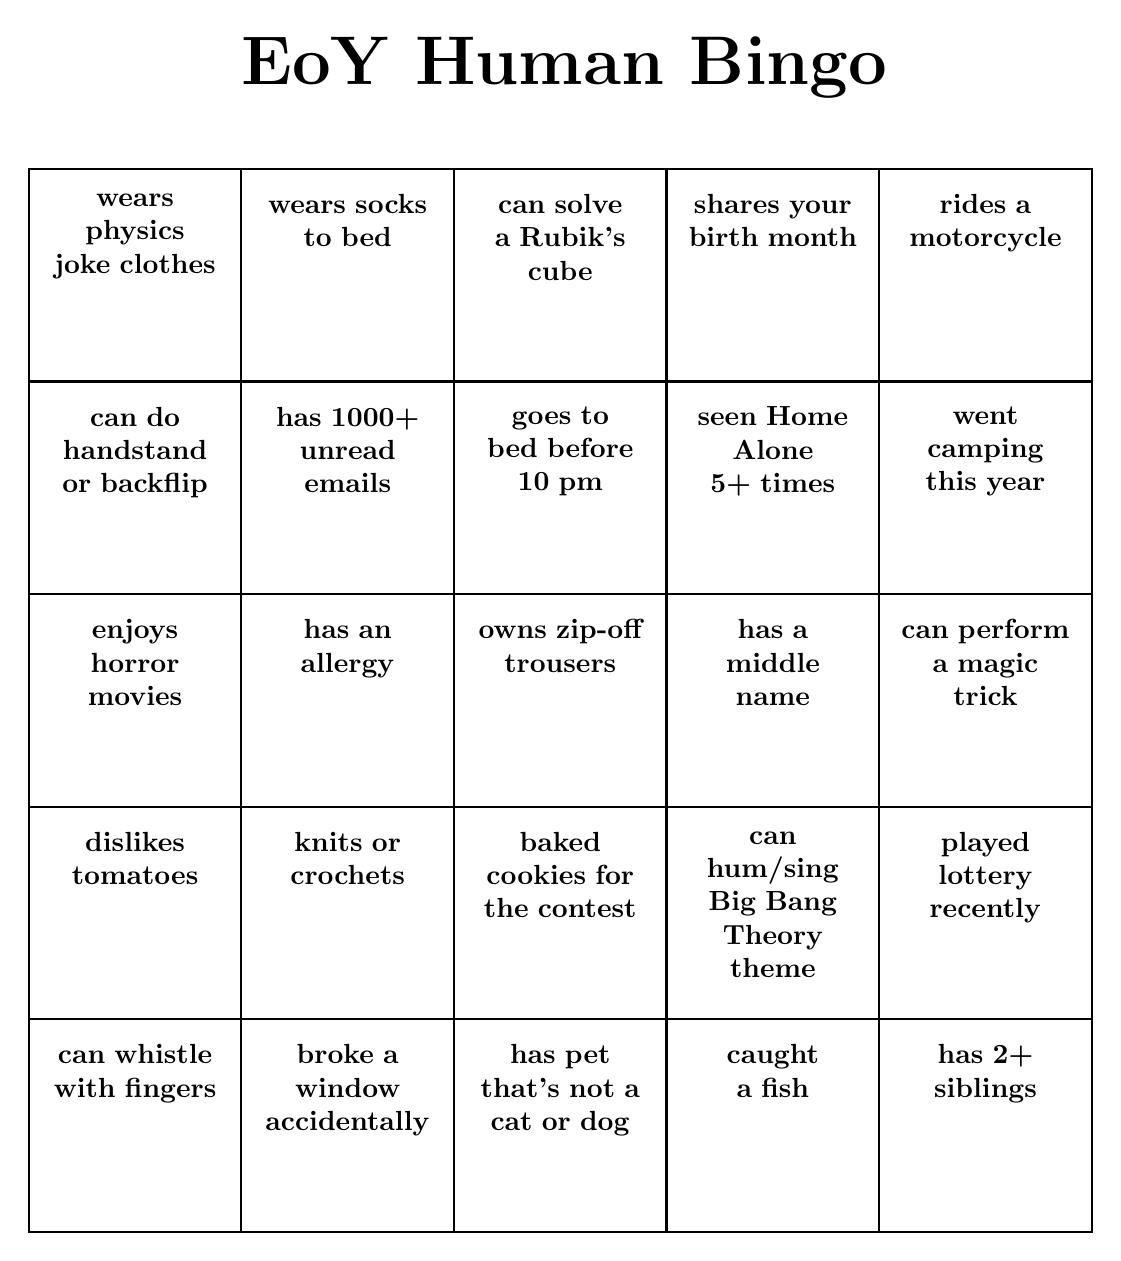
\begin{tikzpicture}
% Set the grid dimensions
\def\cellsize{2.7cm} % Each cell will be 2x2 cm

% Draw the grid and insert the numbers
\draw[thick] (0.0, 0.0) rectangle +(2.7, 2.7);
\node[anchor=north, align=center, text width=2.2cm] at (1.35, 2.5) {\textbf{wears physics joke clothes}};
\draw[thick] (2.7, 0.0) rectangle +(2.7, 2.7);
\node[anchor=north, align=center, text width=2.2cm] at (4.050000000000001, 2.5) {\textbf{wears socks to bed}};
\draw[thick] (5.4, 0.0) rectangle +(2.7, 2.7);
\node[anchor=north, align=center, text width=2.2cm] at (6.75, 2.5) {\textbf{can solve a Rubik's cube}};
\draw[thick] (8.100000000000001, 0.0) rectangle +(2.7, 2.7);
\node[anchor=north, align=center, text width=2.2cm] at (9.450000000000001, 2.5) {\textbf{shares your birth month}};
\draw[thick] (10.8, 0.0) rectangle +(2.7, 2.7);
\node[anchor=north, align=center, text width=2.2cm] at (12.15, 2.5) {\textbf{rides a motorcycle}};
\draw[thick] (0.0, -2.7) rectangle +(2.7, 2.7);
\node[anchor=north, align=center, text width=2.2cm] at (1.35, -0.2) {\textbf{can do handstand or backflip}};
\draw[thick] (2.7, -2.7) rectangle +(2.7, 2.7);
\node[anchor=north, align=center, text width=2.2cm] at (4.050000000000001, -0.2) {\textbf{has 1000+ unread emails}};
\draw[thick] (5.4, -2.7) rectangle +(2.7, 2.7);
\node[anchor=north, align=center, text width=2.2cm] at (6.75, -0.2) {\textbf{goes to bed before 10 pm}};
\draw[thick] (8.100000000000001, -2.7) rectangle +(2.7, 2.7);
\node[anchor=north, align=center, text width=2.2cm] at (9.450000000000001, -0.2) {\textbf{seen Home Alone 5+ times}};
\draw[thick] (10.8, -2.7) rectangle +(2.7, 2.7);
\node[anchor=north, align=center, text width=2.2cm] at (12.15, -0.2) {\textbf{went camping this year}};
\draw[thick] (0.0, -5.4) rectangle +(2.7, 2.7);
\node[anchor=north, align=center, text width=2.2cm] at (1.35, -2.9000000000000004) {\textbf{enjoys horror movies}};
\draw[thick] (2.7, -5.4) rectangle +(2.7, 2.7);
\node[anchor=north, align=center, text width=2.2cm] at (4.050000000000001, -2.9000000000000004) {\textbf{has an allergy}};
\draw[thick] (5.4, -5.4) rectangle +(2.7, 2.7);
\node[anchor=north, align=center, text width=2.2cm] at (6.75, -2.9000000000000004) {\textbf{owns zip-off trousers}};
\draw[thick] (8.100000000000001, -5.4) rectangle +(2.7, 2.7);
\node[anchor=north, align=center, text width=2.2cm] at (9.450000000000001, -2.9000000000000004) {\textbf{has a middle name}};
\draw[thick] (10.8, -5.4) rectangle +(2.7, 2.7);
\node[anchor=north, align=center, text width=2.2cm] at (12.15, -2.9000000000000004) {\textbf{can perform a magic trick}};
\draw[thick] (0.0, -8.100000000000001) rectangle +(2.7, 2.7);
\node[anchor=north, align=center, text width=2.2cm] at (1.35, -5.600000000000001) {\textbf{dislikes tomatoes}};
\draw[thick] (2.7, -8.100000000000001) rectangle +(2.7, 2.7);
\node[anchor=north, align=center, text width=2.2cm] at (4.050000000000001, -5.600000000000001) {\textbf{knits or crochets}};
\draw[thick] (5.4, -8.100000000000001) rectangle +(2.7, 2.7);
\node[anchor=north, align=center, text width=2.2cm] at (6.75, -5.600000000000001) {\textbf{baked cookies for the contest}};
\draw[thick] (8.100000000000001, -8.100000000000001) rectangle +(2.7, 2.7);
\node[anchor=north, align=center, text width=2.2cm] at (9.450000000000001, -5.600000000000001) {\textbf{can hum/sing Big Bang Theory theme}};
\draw[thick] (10.8, -8.100000000000001) rectangle +(2.7, 2.7);
\node[anchor=north, align=center, text width=2.2cm] at (12.15, -5.600000000000001) {\textbf{played lottery recently}};
\draw[thick] (0.0, -10.8) rectangle +(2.7, 2.7);
\node[anchor=north, align=center, text width=2.2cm] at (1.35, -8.3) {\textbf{can whistle with fingers}};
\draw[thick] (2.7, -10.8) rectangle +(2.7, 2.7);
\node[anchor=north, align=center, text width=2.2cm] at (4.050000000000001, -8.3) {\textbf{broke a window accidentally}};
\draw[thick] (5.4, -10.8) rectangle +(2.7, 2.7);
\node[anchor=north, align=center, text width=2.2cm] at (6.75, -8.3) {\textbf{has pet that's not a cat or dog}};
\draw[thick] (8.100000000000001, -10.8) rectangle +(2.7, 2.7);
\node[anchor=north, align=center, text width=2.2cm] at (9.450000000000001, -8.3) {\textbf{caught a fish}};
\draw[thick] (10.8, -10.8) rectangle +(2.7, 2.7);
\node[anchor=north, align=center, text width=2.2cm] at (12.15, -8.3) {\textbf{has 2+ siblings}};
\node[anchor=north, font = \Huge] at (6.8, 4.5){\textbf{EoY Human Bingo}};
\end{tikzpicture}
\end{center}
\newpage\begin{center}
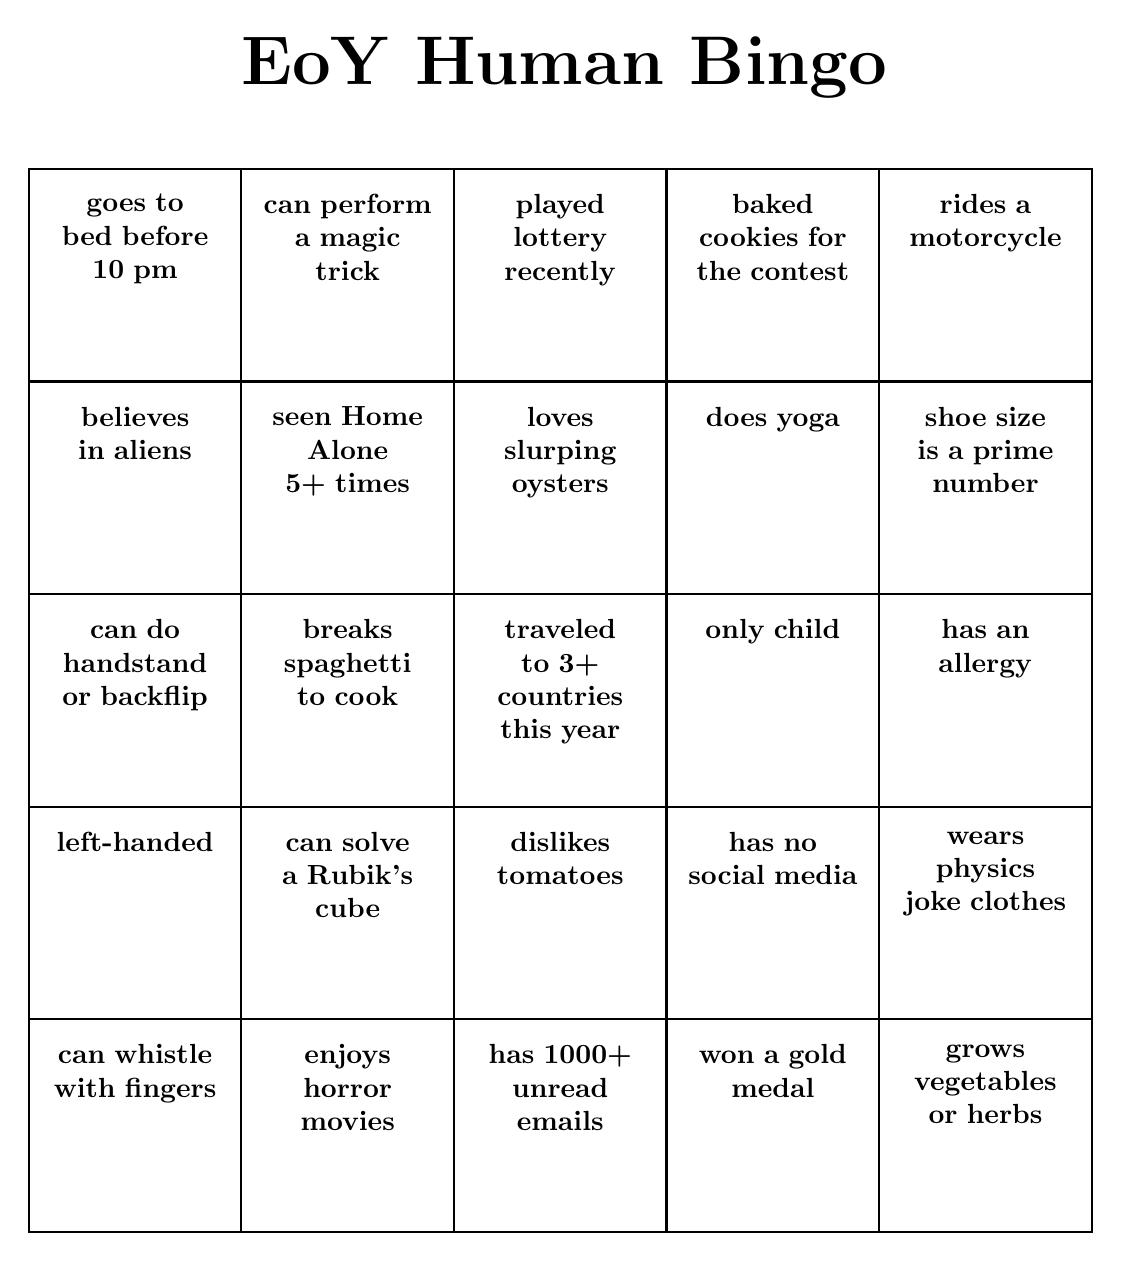
\begin{tikzpicture}
% Set the grid dimensions
\def\cellsize{2.7cm} % Each cell will be 2x2 cm

% Draw the grid and insert the numbers
\draw[thick] (0.0, 0.0) rectangle +(2.7, 2.7);
\node[anchor=north, align=center, text width=2.2cm] at (1.35, 2.5) {\textbf{goes to bed before 10 pm}};
\draw[thick] (2.7, 0.0) rectangle +(2.7, 2.7);
\node[anchor=north, align=center, text width=2.2cm] at (4.050000000000001, 2.5) {\textbf{can perform a magic trick}};
\draw[thick] (5.4, 0.0) rectangle +(2.7, 2.7);
\node[anchor=north, align=center, text width=2.2cm] at (6.75, 2.5) {\textbf{played lottery recently}};
\draw[thick] (8.100000000000001, 0.0) rectangle +(2.7, 2.7);
\node[anchor=north, align=center, text width=2.2cm] at (9.450000000000001, 2.5) {\textbf{baked cookies for the contest}};
\draw[thick] (10.8, 0.0) rectangle +(2.7, 2.7);
\node[anchor=north, align=center, text width=2.2cm] at (12.15, 2.5) {\textbf{rides a motorcycle}};
\draw[thick] (0.0, -2.7) rectangle +(2.7, 2.7);
\node[anchor=north, align=center, text width=2.2cm] at (1.35, -0.2) {\textbf{believes in aliens}};
\draw[thick] (2.7, -2.7) rectangle +(2.7, 2.7);
\node[anchor=north, align=center, text width=2.2cm] at (4.050000000000001, -0.2) {\textbf{seen Home Alone 5+ times}};
\draw[thick] (5.4, -2.7) rectangle +(2.7, 2.7);
\node[anchor=north, align=center, text width=2.2cm] at (6.75, -0.2) {\textbf{loves slurping oysters}};
\draw[thick] (8.100000000000001, -2.7) rectangle +(2.7, 2.7);
\node[anchor=north, align=center, text width=2.2cm] at (9.450000000000001, -0.2) {\textbf{does yoga}};
\draw[thick] (10.8, -2.7) rectangle +(2.7, 2.7);
\node[anchor=north, align=center, text width=2.2cm] at (12.15, -0.2) {\textbf{shoe size is a prime number}};
\draw[thick] (0.0, -5.4) rectangle +(2.7, 2.7);
\node[anchor=north, align=center, text width=2.2cm] at (1.35, -2.9000000000000004) {\textbf{can do handstand or backflip}};
\draw[thick] (2.7, -5.4) rectangle +(2.7, 2.7);
\node[anchor=north, align=center, text width=2.2cm] at (4.050000000000001, -2.9000000000000004) {\textbf{breaks spaghetti to cook}};
\draw[thick] (5.4, -5.4) rectangle +(2.7, 2.7);
\node[anchor=north, align=center, text width=2.2cm] at (6.75, -2.9000000000000004) {\textbf{traveled to 3+ countries this year}};
\draw[thick] (8.100000000000001, -5.4) rectangle +(2.7, 2.7);
\node[anchor=north, align=center, text width=2.2cm] at (9.450000000000001, -2.9000000000000004) {\textbf{only child}};
\draw[thick] (10.8, -5.4) rectangle +(2.7, 2.7);
\node[anchor=north, align=center, text width=2.2cm] at (12.15, -2.9000000000000004) {\textbf{has an allergy}};
\draw[thick] (0.0, -8.100000000000001) rectangle +(2.7, 2.7);
\node[anchor=north, align=center, text width=2.2cm] at (1.35, -5.600000000000001) {\textbf{left-handed}};
\draw[thick] (2.7, -8.100000000000001) rectangle +(2.7, 2.7);
\node[anchor=north, align=center, text width=2.2cm] at (4.050000000000001, -5.600000000000001) {\textbf{can solve a Rubik's cube}};
\draw[thick] (5.4, -8.100000000000001) rectangle +(2.7, 2.7);
\node[anchor=north, align=center, text width=2.2cm] at (6.75, -5.600000000000001) {\textbf{dislikes tomatoes}};
\draw[thick] (8.100000000000001, -8.100000000000001) rectangle +(2.7, 2.7);
\node[anchor=north, align=center, text width=2.2cm] at (9.450000000000001, -5.600000000000001) {\textbf{has no social media}};
\draw[thick] (10.8, -8.100000000000001) rectangle +(2.7, 2.7);
\node[anchor=north, align=center, text width=2.2cm] at (12.15, -5.600000000000001) {\textbf{wears physics joke clothes}};
\draw[thick] (0.0, -10.8) rectangle +(2.7, 2.7);
\node[anchor=north, align=center, text width=2.2cm] at (1.35, -8.3) {\textbf{can whistle with fingers}};
\draw[thick] (2.7, -10.8) rectangle +(2.7, 2.7);
\node[anchor=north, align=center, text width=2.2cm] at (4.050000000000001, -8.3) {\textbf{enjoys horror movies}};
\draw[thick] (5.4, -10.8) rectangle +(2.7, 2.7);
\node[anchor=north, align=center, text width=2.2cm] at (6.75, -8.3) {\textbf{has 1000+ unread emails}};
\draw[thick] (8.100000000000001, -10.8) rectangle +(2.7, 2.7);
\node[anchor=north, align=center, text width=2.2cm] at (9.450000000000001, -8.3) {\textbf{won a gold medal}};
\draw[thick] (10.8, -10.8) rectangle +(2.7, 2.7);
\node[anchor=north, align=center, text width=2.2cm] at (12.15, -8.3) {\textbf{grows vegetables or herbs}};
\node[anchor=north, font = \Huge] at (6.8, 4.5){\textbf{EoY Human Bingo}};
\end{tikzpicture}
\end{center}
\newpage\begin{center}
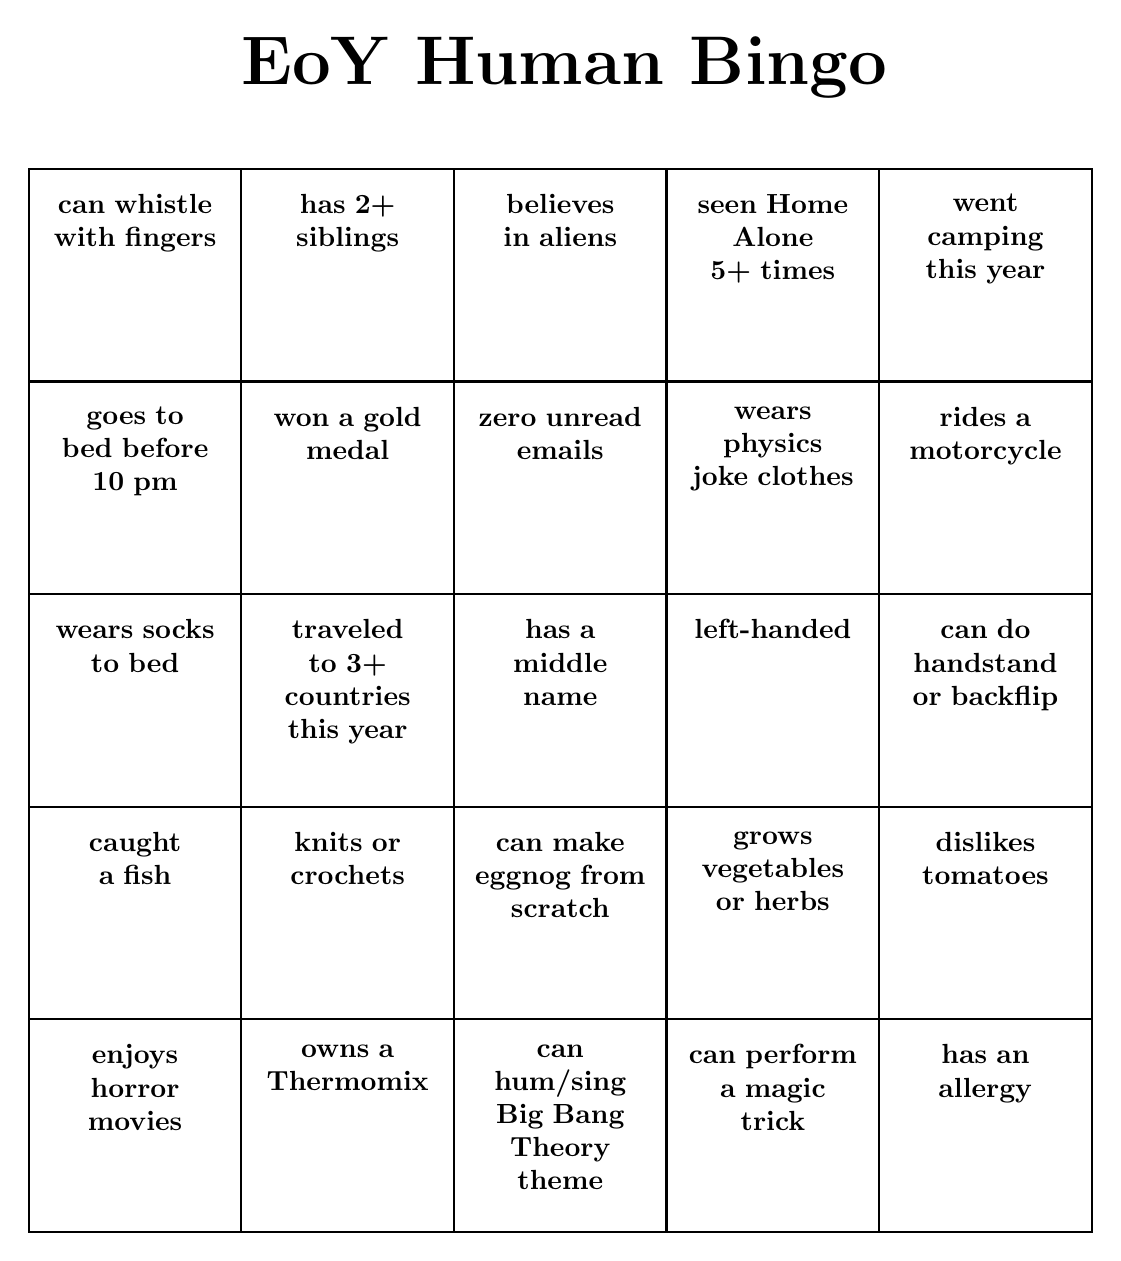
\begin{tikzpicture}
% Set the grid dimensions
\def\cellsize{2.7cm} % Each cell will be 2x2 cm

% Draw the grid and insert the numbers
\draw[thick] (0.0, 0.0) rectangle +(2.7, 2.7);
\node[anchor=north, align=center, text width=2.2cm] at (1.35, 2.5) {\textbf{can whistle with fingers}};
\draw[thick] (2.7, 0.0) rectangle +(2.7, 2.7);
\node[anchor=north, align=center, text width=2.2cm] at (4.050000000000001, 2.5) {\textbf{has 2+ siblings}};
\draw[thick] (5.4, 0.0) rectangle +(2.7, 2.7);
\node[anchor=north, align=center, text width=2.2cm] at (6.75, 2.5) {\textbf{believes in aliens}};
\draw[thick] (8.100000000000001, 0.0) rectangle +(2.7, 2.7);
\node[anchor=north, align=center, text width=2.2cm] at (9.450000000000001, 2.5) {\textbf{seen Home Alone 5+ times}};
\draw[thick] (10.8, 0.0) rectangle +(2.7, 2.7);
\node[anchor=north, align=center, text width=2.2cm] at (12.15, 2.5) {\textbf{went camping this year}};
\draw[thick] (0.0, -2.7) rectangle +(2.7, 2.7);
\node[anchor=north, align=center, text width=2.2cm] at (1.35, -0.2) {\textbf{goes to bed before 10 pm}};
\draw[thick] (2.7, -2.7) rectangle +(2.7, 2.7);
\node[anchor=north, align=center, text width=2.2cm] at (4.050000000000001, -0.2) {\textbf{won a gold medal}};
\draw[thick] (5.4, -2.7) rectangle +(2.7, 2.7);
\node[anchor=north, align=center, text width=2.2cm] at (6.75, -0.2) {\textbf{zero unread emails}};
\draw[thick] (8.100000000000001, -2.7) rectangle +(2.7, 2.7);
\node[anchor=north, align=center, text width=2.2cm] at (9.450000000000001, -0.2) {\textbf{wears physics joke clothes}};
\draw[thick] (10.8, -2.7) rectangle +(2.7, 2.7);
\node[anchor=north, align=center, text width=2.2cm] at (12.15, -0.2) {\textbf{rides a motorcycle}};
\draw[thick] (0.0, -5.4) rectangle +(2.7, 2.7);
\node[anchor=north, align=center, text width=2.2cm] at (1.35, -2.9000000000000004) {\textbf{wears socks to bed}};
\draw[thick] (2.7, -5.4) rectangle +(2.7, 2.7);
\node[anchor=north, align=center, text width=2.2cm] at (4.050000000000001, -2.9000000000000004) {\textbf{traveled to 3+ countries this year}};
\draw[thick] (5.4, -5.4) rectangle +(2.7, 2.7);
\node[anchor=north, align=center, text width=2.2cm] at (6.75, -2.9000000000000004) {\textbf{has a middle name}};
\draw[thick] (8.100000000000001, -5.4) rectangle +(2.7, 2.7);
\node[anchor=north, align=center, text width=2.2cm] at (9.450000000000001, -2.9000000000000004) {\textbf{left-handed}};
\draw[thick] (10.8, -5.4) rectangle +(2.7, 2.7);
\node[anchor=north, align=center, text width=2.2cm] at (12.15, -2.9000000000000004) {\textbf{can do handstand or backflip}};
\draw[thick] (0.0, -8.100000000000001) rectangle +(2.7, 2.7);
\node[anchor=north, align=center, text width=2.2cm] at (1.35, -5.600000000000001) {\textbf{caught a fish}};
\draw[thick] (2.7, -8.100000000000001) rectangle +(2.7, 2.7);
\node[anchor=north, align=center, text width=2.2cm] at (4.050000000000001, -5.600000000000001) {\textbf{knits or crochets}};
\draw[thick] (5.4, -8.100000000000001) rectangle +(2.7, 2.7);
\node[anchor=north, align=center, text width=2.2cm] at (6.75, -5.600000000000001) {\textbf{can make eggnog from scratch}};
\draw[thick] (8.100000000000001, -8.100000000000001) rectangle +(2.7, 2.7);
\node[anchor=north, align=center, text width=2.2cm] at (9.450000000000001, -5.600000000000001) {\textbf{grows vegetables or herbs}};
\draw[thick] (10.8, -8.100000000000001) rectangle +(2.7, 2.7);
\node[anchor=north, align=center, text width=2.2cm] at (12.15, -5.600000000000001) {\textbf{dislikes tomatoes}};
\draw[thick] (0.0, -10.8) rectangle +(2.7, 2.7);
\node[anchor=north, align=center, text width=2.2cm] at (1.35, -8.3) {\textbf{enjoys horror movies}};
\draw[thick] (2.7, -10.8) rectangle +(2.7, 2.7);
\node[anchor=north, align=center, text width=2.2cm] at (4.050000000000001, -8.3) {\textbf{owns a Thermomix}};
\draw[thick] (5.4, -10.8) rectangle +(2.7, 2.7);
\node[anchor=north, align=center, text width=2.2cm] at (6.75, -8.3) {\textbf{can hum/sing Big Bang Theory theme}};
\draw[thick] (8.100000000000001, -10.8) rectangle +(2.7, 2.7);
\node[anchor=north, align=center, text width=2.2cm] at (9.450000000000001, -8.3) {\textbf{can perform a magic trick}};
\draw[thick] (10.8, -10.8) rectangle +(2.7, 2.7);
\node[anchor=north, align=center, text width=2.2cm] at (12.15, -8.3) {\textbf{has an allergy}};
\node[anchor=north, font = \Huge] at (6.8, 4.5){\textbf{EoY Human Bingo}};
\end{tikzpicture}
\end{center}
\newpage\begin{center}
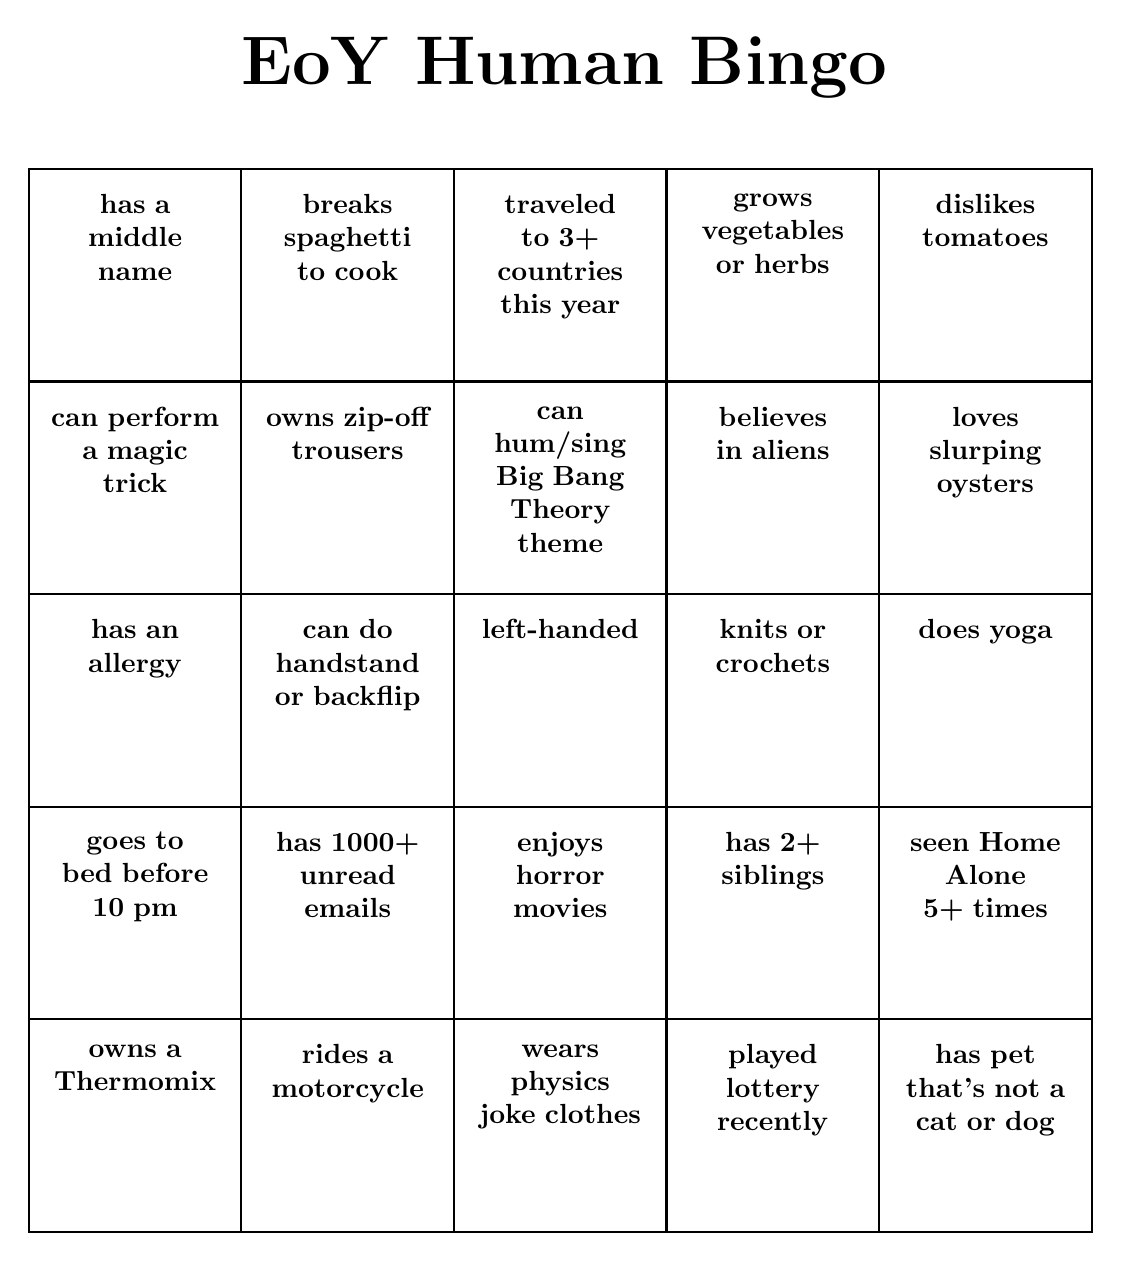
\begin{tikzpicture}
% Set the grid dimensions
\def\cellsize{2.7cm} % Each cell will be 2x2 cm

% Draw the grid and insert the numbers
\draw[thick] (0.0, 0.0) rectangle +(2.7, 2.7);
\node[anchor=north, align=center, text width=2.2cm] at (1.35, 2.5) {\textbf{has a middle name}};
\draw[thick] (2.7, 0.0) rectangle +(2.7, 2.7);
\node[anchor=north, align=center, text width=2.2cm] at (4.050000000000001, 2.5) {\textbf{breaks spaghetti to cook}};
\draw[thick] (5.4, 0.0) rectangle +(2.7, 2.7);
\node[anchor=north, align=center, text width=2.2cm] at (6.75, 2.5) {\textbf{traveled to 3+ countries this year}};
\draw[thick] (8.100000000000001, 0.0) rectangle +(2.7, 2.7);
\node[anchor=north, align=center, text width=2.2cm] at (9.450000000000001, 2.5) {\textbf{grows vegetables or herbs}};
\draw[thick] (10.8, 0.0) rectangle +(2.7, 2.7);
\node[anchor=north, align=center, text width=2.2cm] at (12.15, 2.5) {\textbf{dislikes tomatoes}};
\draw[thick] (0.0, -2.7) rectangle +(2.7, 2.7);
\node[anchor=north, align=center, text width=2.2cm] at (1.35, -0.2) {\textbf{can perform a magic trick}};
\draw[thick] (2.7, -2.7) rectangle +(2.7, 2.7);
\node[anchor=north, align=center, text width=2.2cm] at (4.050000000000001, -0.2) {\textbf{owns zip-off trousers}};
\draw[thick] (5.4, -2.7) rectangle +(2.7, 2.7);
\node[anchor=north, align=center, text width=2.2cm] at (6.75, -0.2) {\textbf{can hum/sing Big Bang Theory theme}};
\draw[thick] (8.100000000000001, -2.7) rectangle +(2.7, 2.7);
\node[anchor=north, align=center, text width=2.2cm] at (9.450000000000001, -0.2) {\textbf{believes in aliens}};
\draw[thick] (10.8, -2.7) rectangle +(2.7, 2.7);
\node[anchor=north, align=center, text width=2.2cm] at (12.15, -0.2) {\textbf{loves slurping oysters}};
\draw[thick] (0.0, -5.4) rectangle +(2.7, 2.7);
\node[anchor=north, align=center, text width=2.2cm] at (1.35, -2.9000000000000004) {\textbf{has an allergy}};
\draw[thick] (2.7, -5.4) rectangle +(2.7, 2.7);
\node[anchor=north, align=center, text width=2.2cm] at (4.050000000000001, -2.9000000000000004) {\textbf{can do handstand or backflip}};
\draw[thick] (5.4, -5.4) rectangle +(2.7, 2.7);
\node[anchor=north, align=center, text width=2.2cm] at (6.75, -2.9000000000000004) {\textbf{left-handed}};
\draw[thick] (8.100000000000001, -5.4) rectangle +(2.7, 2.7);
\node[anchor=north, align=center, text width=2.2cm] at (9.450000000000001, -2.9000000000000004) {\textbf{knits or crochets}};
\draw[thick] (10.8, -5.4) rectangle +(2.7, 2.7);
\node[anchor=north, align=center, text width=2.2cm] at (12.15, -2.9000000000000004) {\textbf{does yoga}};
\draw[thick] (0.0, -8.100000000000001) rectangle +(2.7, 2.7);
\node[anchor=north, align=center, text width=2.2cm] at (1.35, -5.600000000000001) {\textbf{goes to bed before 10 pm}};
\draw[thick] (2.7, -8.100000000000001) rectangle +(2.7, 2.7);
\node[anchor=north, align=center, text width=2.2cm] at (4.050000000000001, -5.600000000000001) {\textbf{has 1000+ unread emails}};
\draw[thick] (5.4, -8.100000000000001) rectangle +(2.7, 2.7);
\node[anchor=north, align=center, text width=2.2cm] at (6.75, -5.600000000000001) {\textbf{enjoys horror movies}};
\draw[thick] (8.100000000000001, -8.100000000000001) rectangle +(2.7, 2.7);
\node[anchor=north, align=center, text width=2.2cm] at (9.450000000000001, -5.600000000000001) {\textbf{has 2+ siblings}};
\draw[thick] (10.8, -8.100000000000001) rectangle +(2.7, 2.7);
\node[anchor=north, align=center, text width=2.2cm] at (12.15, -5.600000000000001) {\textbf{seen Home Alone 5+ times}};
\draw[thick] (0.0, -10.8) rectangle +(2.7, 2.7);
\node[anchor=north, align=center, text width=2.2cm] at (1.35, -8.3) {\textbf{owns a Thermomix}};
\draw[thick] (2.7, -10.8) rectangle +(2.7, 2.7);
\node[anchor=north, align=center, text width=2.2cm] at (4.050000000000001, -8.3) {\textbf{rides a motorcycle}};
\draw[thick] (5.4, -10.8) rectangle +(2.7, 2.7);
\node[anchor=north, align=center, text width=2.2cm] at (6.75, -8.3) {\textbf{wears physics joke clothes}};
\draw[thick] (8.100000000000001, -10.8) rectangle +(2.7, 2.7);
\node[anchor=north, align=center, text width=2.2cm] at (9.450000000000001, -8.3) {\textbf{played lottery recently}};
\draw[thick] (10.8, -10.8) rectangle +(2.7, 2.7);
\node[anchor=north, align=center, text width=2.2cm] at (12.15, -8.3) {\textbf{has pet that's not a cat or dog}};
\node[anchor=north, font = \Huge] at (6.8, 4.5){\textbf{EoY Human Bingo}};
\end{tikzpicture}
\end{center}
\newpage\begin{center}
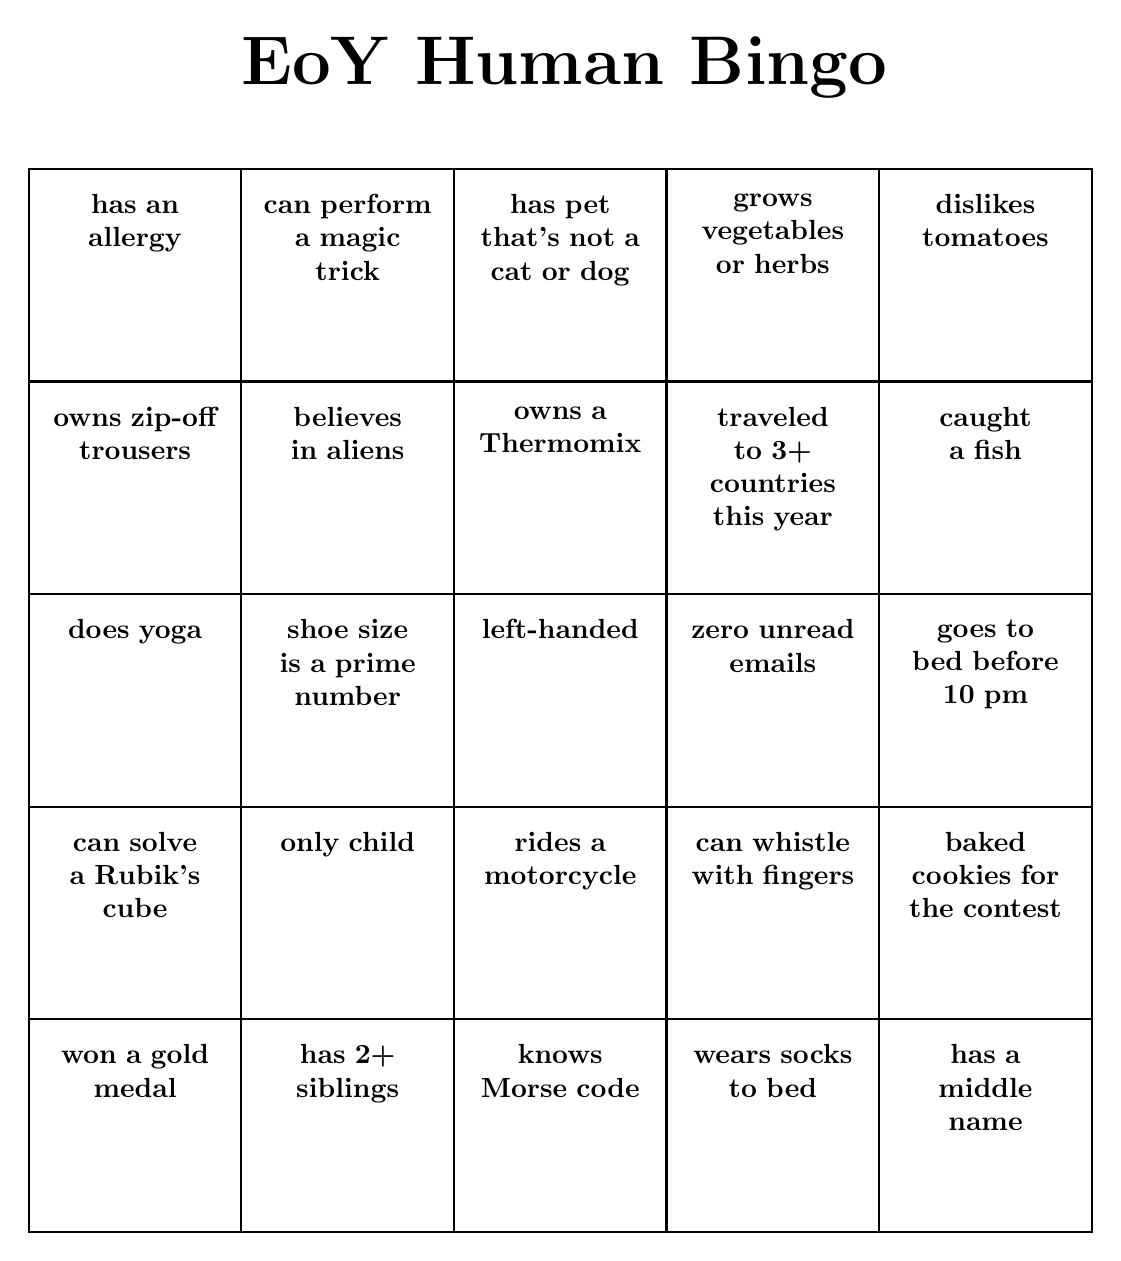
\begin{tikzpicture}
% Set the grid dimensions
\def\cellsize{2.7cm} % Each cell will be 2x2 cm

% Draw the grid and insert the numbers
\draw[thick] (0.0, 0.0) rectangle +(2.7, 2.7);
\node[anchor=north, align=center, text width=2.2cm] at (1.35, 2.5) {\textbf{has an allergy}};
\draw[thick] (2.7, 0.0) rectangle +(2.7, 2.7);
\node[anchor=north, align=center, text width=2.2cm] at (4.050000000000001, 2.5) {\textbf{can perform a magic trick}};
\draw[thick] (5.4, 0.0) rectangle +(2.7, 2.7);
\node[anchor=north, align=center, text width=2.2cm] at (6.75, 2.5) {\textbf{has pet that's not a cat or dog}};
\draw[thick] (8.100000000000001, 0.0) rectangle +(2.7, 2.7);
\node[anchor=north, align=center, text width=2.2cm] at (9.450000000000001, 2.5) {\textbf{grows vegetables or herbs}};
\draw[thick] (10.8, 0.0) rectangle +(2.7, 2.7);
\node[anchor=north, align=center, text width=2.2cm] at (12.15, 2.5) {\textbf{dislikes tomatoes}};
\draw[thick] (0.0, -2.7) rectangle +(2.7, 2.7);
\node[anchor=north, align=center, text width=2.2cm] at (1.35, -0.2) {\textbf{owns zip-off trousers}};
\draw[thick] (2.7, -2.7) rectangle +(2.7, 2.7);
\node[anchor=north, align=center, text width=2.2cm] at (4.050000000000001, -0.2) {\textbf{believes in aliens}};
\draw[thick] (5.4, -2.7) rectangle +(2.7, 2.7);
\node[anchor=north, align=center, text width=2.2cm] at (6.75, -0.2) {\textbf{owns a Thermomix}};
\draw[thick] (8.100000000000001, -2.7) rectangle +(2.7, 2.7);
\node[anchor=north, align=center, text width=2.2cm] at (9.450000000000001, -0.2) {\textbf{traveled to 3+ countries this year}};
\draw[thick] (10.8, -2.7) rectangle +(2.7, 2.7);
\node[anchor=north, align=center, text width=2.2cm] at (12.15, -0.2) {\textbf{caught a fish}};
\draw[thick] (0.0, -5.4) rectangle +(2.7, 2.7);
\node[anchor=north, align=center, text width=2.2cm] at (1.35, -2.9000000000000004) {\textbf{does yoga}};
\draw[thick] (2.7, -5.4) rectangle +(2.7, 2.7);
\node[anchor=north, align=center, text width=2.2cm] at (4.050000000000001, -2.9000000000000004) {\textbf{shoe size is a prime number}};
\draw[thick] (5.4, -5.4) rectangle +(2.7, 2.7);
\node[anchor=north, align=center, text width=2.2cm] at (6.75, -2.9000000000000004) {\textbf{left-handed}};
\draw[thick] (8.100000000000001, -5.4) rectangle +(2.7, 2.7);
\node[anchor=north, align=center, text width=2.2cm] at (9.450000000000001, -2.9000000000000004) {\textbf{zero unread emails}};
\draw[thick] (10.8, -5.4) rectangle +(2.7, 2.7);
\node[anchor=north, align=center, text width=2.2cm] at (12.15, -2.9000000000000004) {\textbf{goes to bed before 10 pm}};
\draw[thick] (0.0, -8.100000000000001) rectangle +(2.7, 2.7);
\node[anchor=north, align=center, text width=2.2cm] at (1.35, -5.600000000000001) {\textbf{can solve a Rubik's cube}};
\draw[thick] (2.7, -8.100000000000001) rectangle +(2.7, 2.7);
\node[anchor=north, align=center, text width=2.2cm] at (4.050000000000001, -5.600000000000001) {\textbf{only child}};
\draw[thick] (5.4, -8.100000000000001) rectangle +(2.7, 2.7);
\node[anchor=north, align=center, text width=2.2cm] at (6.75, -5.600000000000001) {\textbf{rides a motorcycle}};
\draw[thick] (8.100000000000001, -8.100000000000001) rectangle +(2.7, 2.7);
\node[anchor=north, align=center, text width=2.2cm] at (9.450000000000001, -5.600000000000001) {\textbf{can whistle with fingers}};
\draw[thick] (10.8, -8.100000000000001) rectangle +(2.7, 2.7);
\node[anchor=north, align=center, text width=2.2cm] at (12.15, -5.600000000000001) {\textbf{baked cookies for the contest}};
\draw[thick] (0.0, -10.8) rectangle +(2.7, 2.7);
\node[anchor=north, align=center, text width=2.2cm] at (1.35, -8.3) {\textbf{won a gold medal}};
\draw[thick] (2.7, -10.8) rectangle +(2.7, 2.7);
\node[anchor=north, align=center, text width=2.2cm] at (4.050000000000001, -8.3) {\textbf{has 2+ siblings}};
\draw[thick] (5.4, -10.8) rectangle +(2.7, 2.7);
\node[anchor=north, align=center, text width=2.2cm] at (6.75, -8.3) {\textbf{knows Morse code}};
\draw[thick] (8.100000000000001, -10.8) rectangle +(2.7, 2.7);
\node[anchor=north, align=center, text width=2.2cm] at (9.450000000000001, -8.3) {\textbf{wears socks to bed}};
\draw[thick] (10.8, -10.8) rectangle +(2.7, 2.7);
\node[anchor=north, align=center, text width=2.2cm] at (12.15, -8.3) {\textbf{has a middle name}};
\node[anchor=north, font = \Huge] at (6.8, 4.5){\textbf{EoY Human Bingo}};
\end{tikzpicture}
\end{center}
\newpage\begin{center}
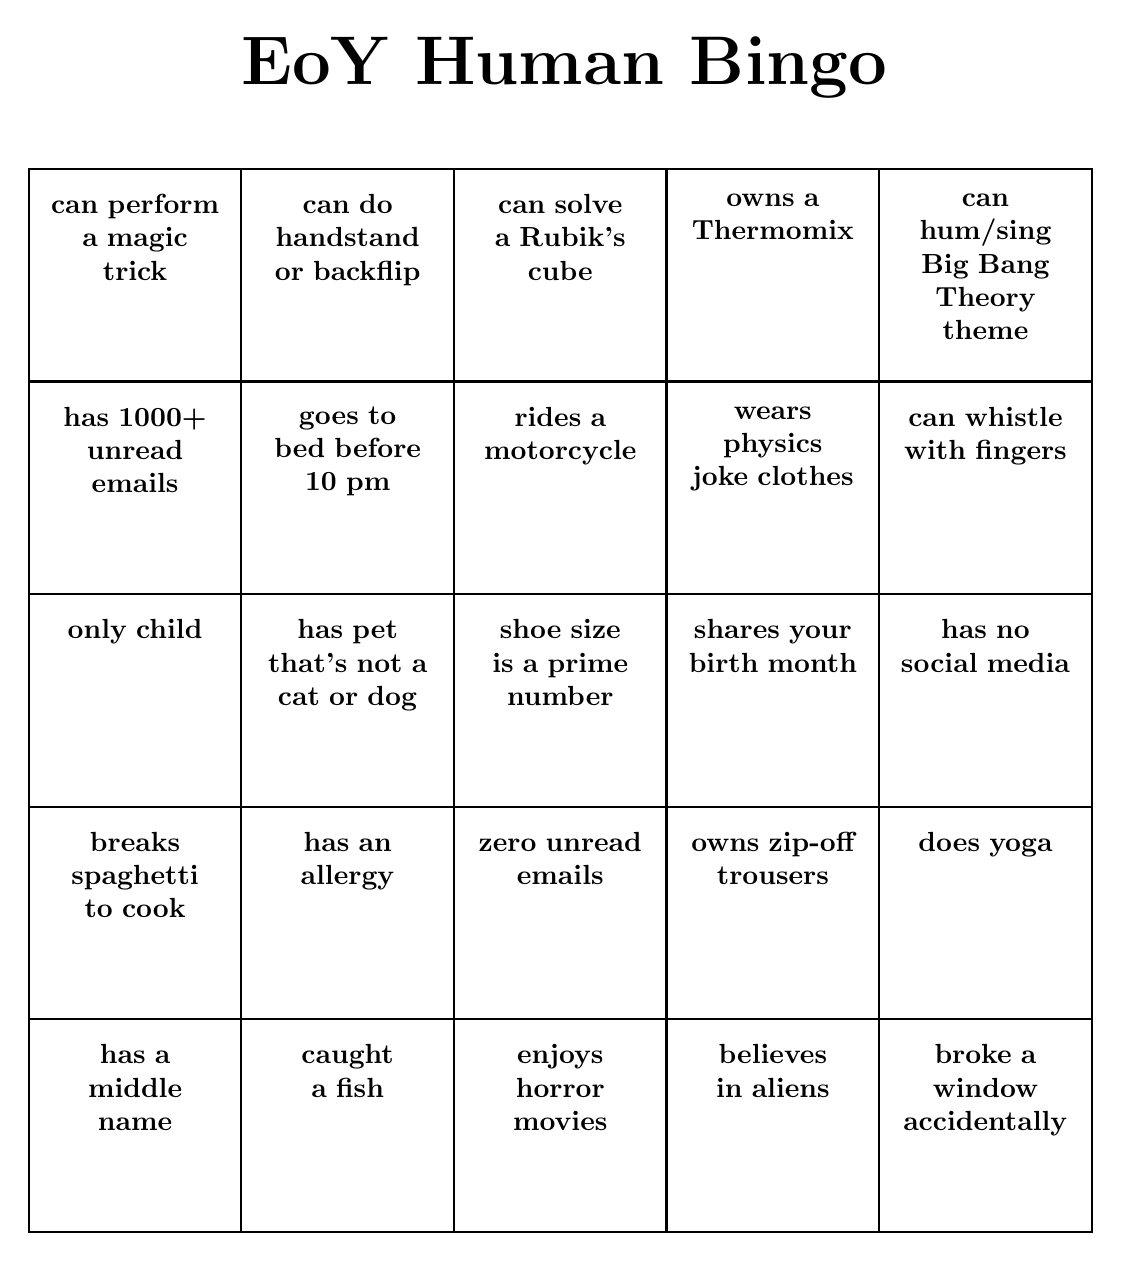
\begin{tikzpicture}
% Set the grid dimensions
\def\cellsize{2.7cm} % Each cell will be 2x2 cm

% Draw the grid and insert the numbers
\draw[thick] (0.0, 0.0) rectangle +(2.7, 2.7);
\node[anchor=north, align=center, text width=2.2cm] at (1.35, 2.5) {\textbf{can perform a magic trick}};
\draw[thick] (2.7, 0.0) rectangle +(2.7, 2.7);
\node[anchor=north, align=center, text width=2.2cm] at (4.050000000000001, 2.5) {\textbf{can do handstand or backflip}};
\draw[thick] (5.4, 0.0) rectangle +(2.7, 2.7);
\node[anchor=north, align=center, text width=2.2cm] at (6.75, 2.5) {\textbf{can solve a Rubik's cube}};
\draw[thick] (8.100000000000001, 0.0) rectangle +(2.7, 2.7);
\node[anchor=north, align=center, text width=2.2cm] at (9.450000000000001, 2.5) {\textbf{owns a Thermomix}};
\draw[thick] (10.8, 0.0) rectangle +(2.7, 2.7);
\node[anchor=north, align=center, text width=2.2cm] at (12.15, 2.5) {\textbf{can hum/sing Big Bang Theory theme}};
\draw[thick] (0.0, -2.7) rectangle +(2.7, 2.7);
\node[anchor=north, align=center, text width=2.2cm] at (1.35, -0.2) {\textbf{has 1000+ unread emails}};
\draw[thick] (2.7, -2.7) rectangle +(2.7, 2.7);
\node[anchor=north, align=center, text width=2.2cm] at (4.050000000000001, -0.2) {\textbf{goes to bed before 10 pm}};
\draw[thick] (5.4, -2.7) rectangle +(2.7, 2.7);
\node[anchor=north, align=center, text width=2.2cm] at (6.75, -0.2) {\textbf{rides a motorcycle}};
\draw[thick] (8.100000000000001, -2.7) rectangle +(2.7, 2.7);
\node[anchor=north, align=center, text width=2.2cm] at (9.450000000000001, -0.2) {\textbf{wears physics joke clothes}};
\draw[thick] (10.8, -2.7) rectangle +(2.7, 2.7);
\node[anchor=north, align=center, text width=2.2cm] at (12.15, -0.2) {\textbf{can whistle with fingers}};
\draw[thick] (0.0, -5.4) rectangle +(2.7, 2.7);
\node[anchor=north, align=center, text width=2.2cm] at (1.35, -2.9000000000000004) {\textbf{only child}};
\draw[thick] (2.7, -5.4) rectangle +(2.7, 2.7);
\node[anchor=north, align=center, text width=2.2cm] at (4.050000000000001, -2.9000000000000004) {\textbf{has pet that's not a cat or dog}};
\draw[thick] (5.4, -5.4) rectangle +(2.7, 2.7);
\node[anchor=north, align=center, text width=2.2cm] at (6.75, -2.9000000000000004) {\textbf{shoe size is a prime number}};
\draw[thick] (8.100000000000001, -5.4) rectangle +(2.7, 2.7);
\node[anchor=north, align=center, text width=2.2cm] at (9.450000000000001, -2.9000000000000004) {\textbf{shares your birth month}};
\draw[thick] (10.8, -5.4) rectangle +(2.7, 2.7);
\node[anchor=north, align=center, text width=2.2cm] at (12.15, -2.9000000000000004) {\textbf{has no social media}};
\draw[thick] (0.0, -8.100000000000001) rectangle +(2.7, 2.7);
\node[anchor=north, align=center, text width=2.2cm] at (1.35, -5.600000000000001) {\textbf{breaks spaghetti to cook}};
\draw[thick] (2.7, -8.100000000000001) rectangle +(2.7, 2.7);
\node[anchor=north, align=center, text width=2.2cm] at (4.050000000000001, -5.600000000000001) {\textbf{has an allergy}};
\draw[thick] (5.4, -8.100000000000001) rectangle +(2.7, 2.7);
\node[anchor=north, align=center, text width=2.2cm] at (6.75, -5.600000000000001) {\textbf{zero unread emails}};
\draw[thick] (8.100000000000001, -8.100000000000001) rectangle +(2.7, 2.7);
\node[anchor=north, align=center, text width=2.2cm] at (9.450000000000001, -5.600000000000001) {\textbf{owns zip-off trousers}};
\draw[thick] (10.8, -8.100000000000001) rectangle +(2.7, 2.7);
\node[anchor=north, align=center, text width=2.2cm] at (12.15, -5.600000000000001) {\textbf{does yoga}};
\draw[thick] (0.0, -10.8) rectangle +(2.7, 2.7);
\node[anchor=north, align=center, text width=2.2cm] at (1.35, -8.3) {\textbf{has a middle name}};
\draw[thick] (2.7, -10.8) rectangle +(2.7, 2.7);
\node[anchor=north, align=center, text width=2.2cm] at (4.050000000000001, -8.3) {\textbf{caught a fish}};
\draw[thick] (5.4, -10.8) rectangle +(2.7, 2.7);
\node[anchor=north, align=center, text width=2.2cm] at (6.75, -8.3) {\textbf{enjoys horror movies}};
\draw[thick] (8.100000000000001, -10.8) rectangle +(2.7, 2.7);
\node[anchor=north, align=center, text width=2.2cm] at (9.450000000000001, -8.3) {\textbf{believes in aliens}};
\draw[thick] (10.8, -10.8) rectangle +(2.7, 2.7);
\node[anchor=north, align=center, text width=2.2cm] at (12.15, -8.3) {\textbf{broke a window accidentally}};
\node[anchor=north, font = \Huge] at (6.8, 4.5){\textbf{EoY Human Bingo}};
\end{tikzpicture}
\end{center}
\newpage\begin{center}
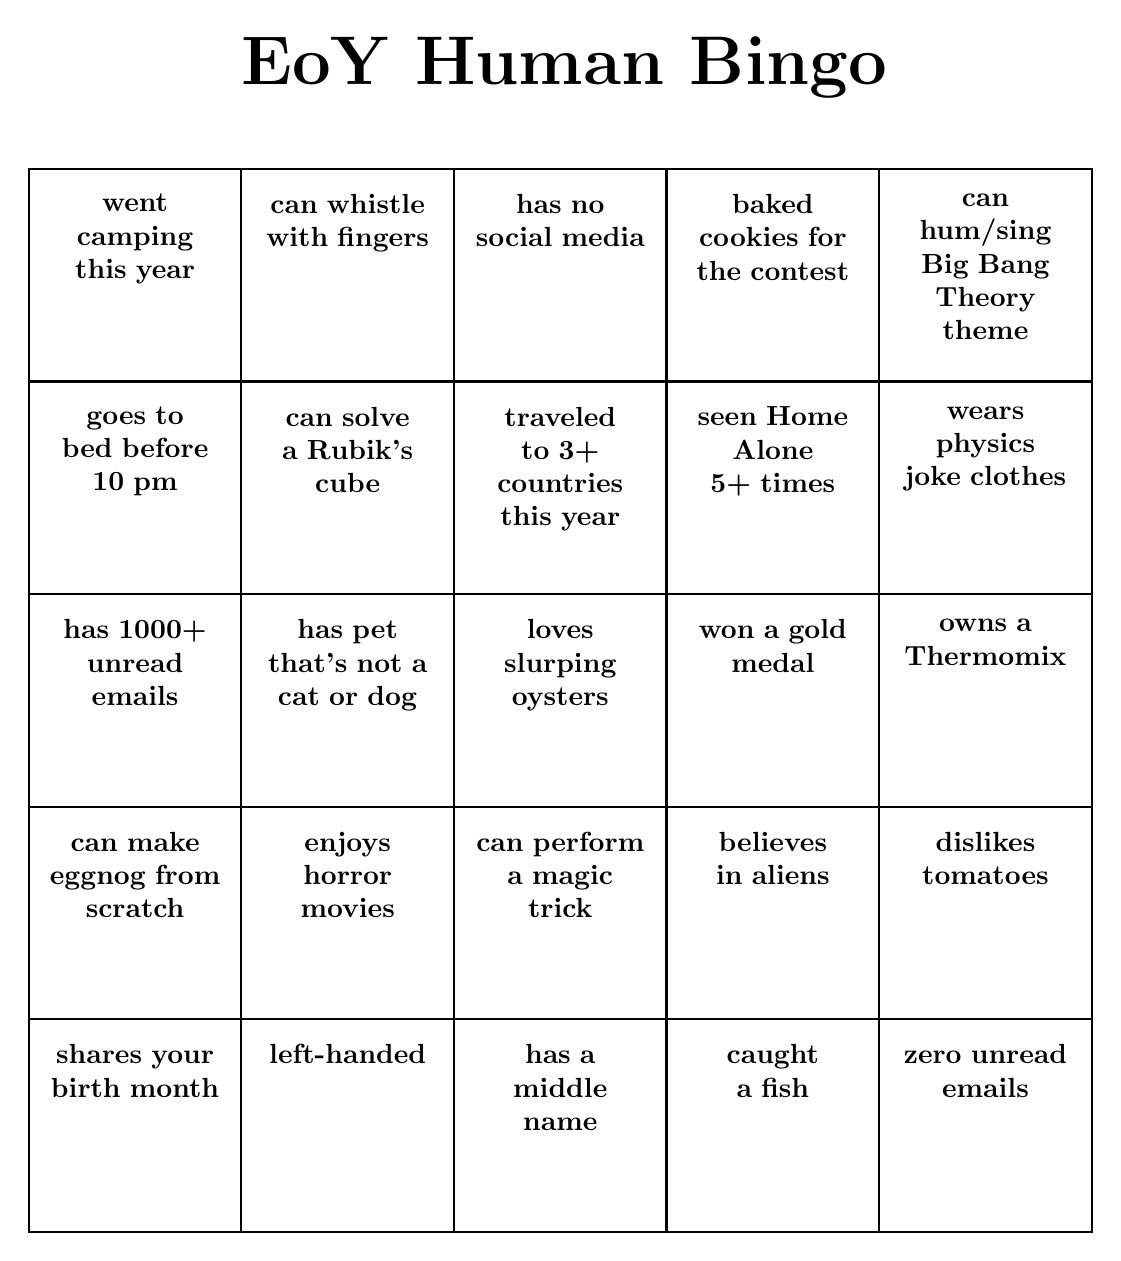
\begin{tikzpicture}
% Set the grid dimensions
\def\cellsize{2.7cm} % Each cell will be 2x2 cm

% Draw the grid and insert the numbers
\draw[thick] (0.0, 0.0) rectangle +(2.7, 2.7);
\node[anchor=north, align=center, text width=2.2cm] at (1.35, 2.5) {\textbf{went camping this year}};
\draw[thick] (2.7, 0.0) rectangle +(2.7, 2.7);
\node[anchor=north, align=center, text width=2.2cm] at (4.050000000000001, 2.5) {\textbf{can whistle with fingers}};
\draw[thick] (5.4, 0.0) rectangle +(2.7, 2.7);
\node[anchor=north, align=center, text width=2.2cm] at (6.75, 2.5) {\textbf{has no social media}};
\draw[thick] (8.100000000000001, 0.0) rectangle +(2.7, 2.7);
\node[anchor=north, align=center, text width=2.2cm] at (9.450000000000001, 2.5) {\textbf{baked cookies for the contest}};
\draw[thick] (10.8, 0.0) rectangle +(2.7, 2.7);
\node[anchor=north, align=center, text width=2.2cm] at (12.15, 2.5) {\textbf{can hum/sing Big Bang Theory theme}};
\draw[thick] (0.0, -2.7) rectangle +(2.7, 2.7);
\node[anchor=north, align=center, text width=2.2cm] at (1.35, -0.2) {\textbf{goes to bed before 10 pm}};
\draw[thick] (2.7, -2.7) rectangle +(2.7, 2.7);
\node[anchor=north, align=center, text width=2.2cm] at (4.050000000000001, -0.2) {\textbf{can solve a Rubik's cube}};
\draw[thick] (5.4, -2.7) rectangle +(2.7, 2.7);
\node[anchor=north, align=center, text width=2.2cm] at (6.75, -0.2) {\textbf{traveled to 3+ countries this year}};
\draw[thick] (8.100000000000001, -2.7) rectangle +(2.7, 2.7);
\node[anchor=north, align=center, text width=2.2cm] at (9.450000000000001, -0.2) {\textbf{seen Home Alone 5+ times}};
\draw[thick] (10.8, -2.7) rectangle +(2.7, 2.7);
\node[anchor=north, align=center, text width=2.2cm] at (12.15, -0.2) {\textbf{wears physics joke clothes}};
\draw[thick] (0.0, -5.4) rectangle +(2.7, 2.7);
\node[anchor=north, align=center, text width=2.2cm] at (1.35, -2.9000000000000004) {\textbf{has 1000+ unread emails}};
\draw[thick] (2.7, -5.4) rectangle +(2.7, 2.7);
\node[anchor=north, align=center, text width=2.2cm] at (4.050000000000001, -2.9000000000000004) {\textbf{has pet that's not a cat or dog}};
\draw[thick] (5.4, -5.4) rectangle +(2.7, 2.7);
\node[anchor=north, align=center, text width=2.2cm] at (6.75, -2.9000000000000004) {\textbf{loves slurping oysters}};
\draw[thick] (8.100000000000001, -5.4) rectangle +(2.7, 2.7);
\node[anchor=north, align=center, text width=2.2cm] at (9.450000000000001, -2.9000000000000004) {\textbf{won a gold medal}};
\draw[thick] (10.8, -5.4) rectangle +(2.7, 2.7);
\node[anchor=north, align=center, text width=2.2cm] at (12.15, -2.9000000000000004) {\textbf{owns a Thermomix}};
\draw[thick] (0.0, -8.100000000000001) rectangle +(2.7, 2.7);
\node[anchor=north, align=center, text width=2.2cm] at (1.35, -5.600000000000001) {\textbf{can make eggnog from scratch}};
\draw[thick] (2.7, -8.100000000000001) rectangle +(2.7, 2.7);
\node[anchor=north, align=center, text width=2.2cm] at (4.050000000000001, -5.600000000000001) {\textbf{enjoys horror movies}};
\draw[thick] (5.4, -8.100000000000001) rectangle +(2.7, 2.7);
\node[anchor=north, align=center, text width=2.2cm] at (6.75, -5.600000000000001) {\textbf{can perform a magic trick}};
\draw[thick] (8.100000000000001, -8.100000000000001) rectangle +(2.7, 2.7);
\node[anchor=north, align=center, text width=2.2cm] at (9.450000000000001, -5.600000000000001) {\textbf{believes in aliens}};
\draw[thick] (10.8, -8.100000000000001) rectangle +(2.7, 2.7);
\node[anchor=north, align=center, text width=2.2cm] at (12.15, -5.600000000000001) {\textbf{dislikes tomatoes}};
\draw[thick] (0.0, -10.8) rectangle +(2.7, 2.7);
\node[anchor=north, align=center, text width=2.2cm] at (1.35, -8.3) {\textbf{shares your birth month}};
\draw[thick] (2.7, -10.8) rectangle +(2.7, 2.7);
\node[anchor=north, align=center, text width=2.2cm] at (4.050000000000001, -8.3) {\textbf{left-handed}};
\draw[thick] (5.4, -10.8) rectangle +(2.7, 2.7);
\node[anchor=north, align=center, text width=2.2cm] at (6.75, -8.3) {\textbf{has a middle name}};
\draw[thick] (8.100000000000001, -10.8) rectangle +(2.7, 2.7);
\node[anchor=north, align=center, text width=2.2cm] at (9.450000000000001, -8.3) {\textbf{caught a fish}};
\draw[thick] (10.8, -10.8) rectangle +(2.7, 2.7);
\node[anchor=north, align=center, text width=2.2cm] at (12.15, -8.3) {\textbf{zero unread emails}};
\node[anchor=north, font = \Huge] at (6.8, 4.5){\textbf{EoY Human Bingo}};
\end{tikzpicture}
\end{center}
\newpage\begin{center}
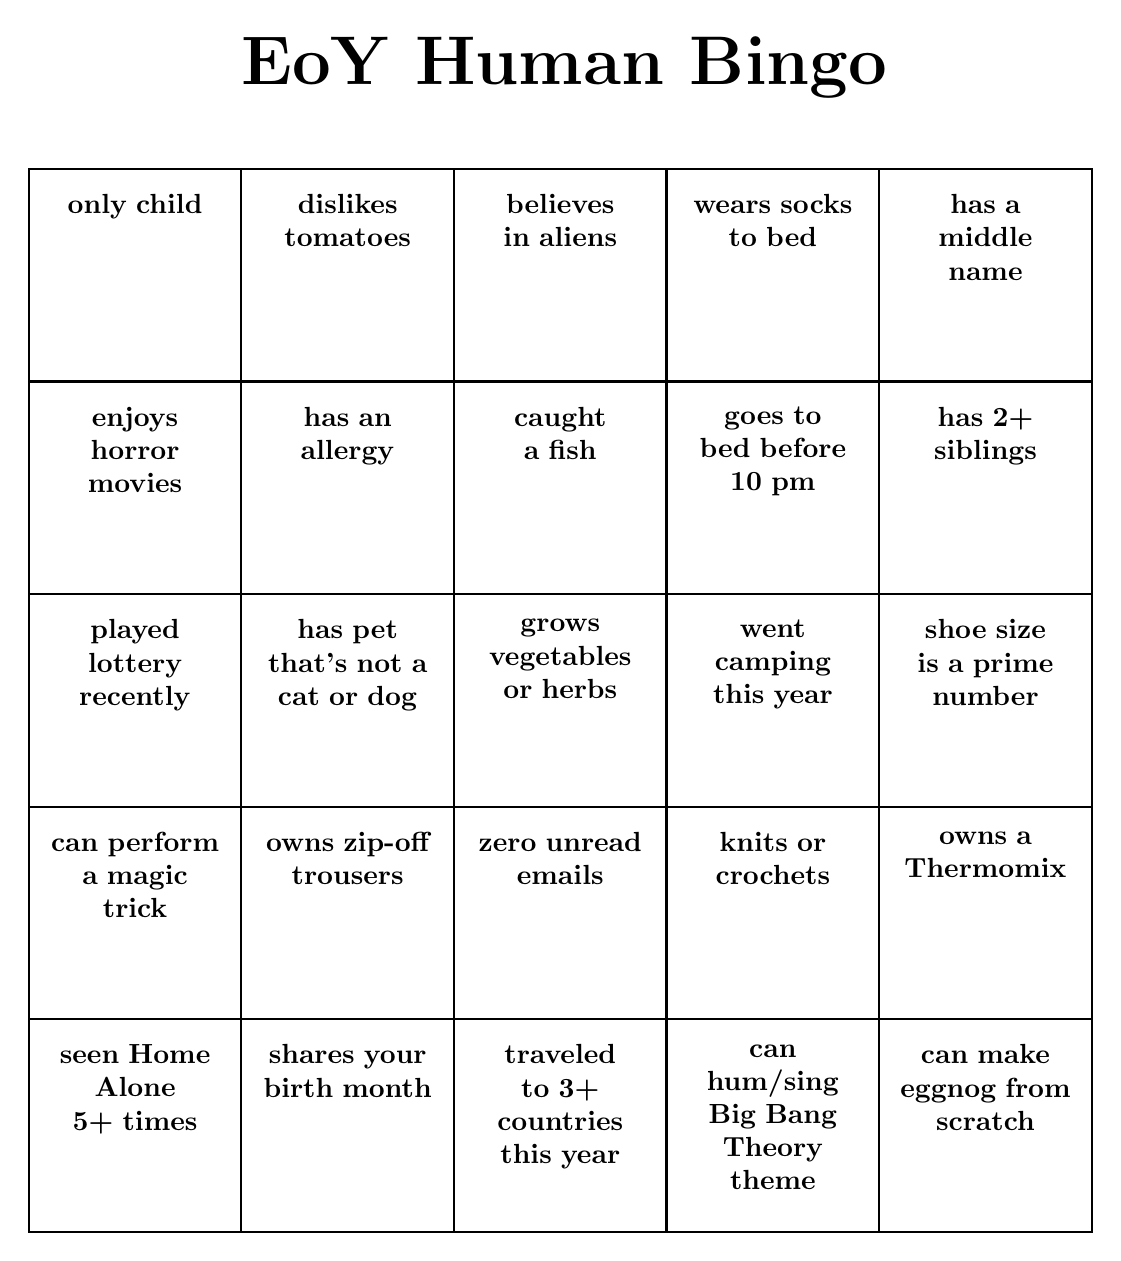
\begin{tikzpicture}
% Set the grid dimensions
\def\cellsize{2.7cm} % Each cell will be 2x2 cm

% Draw the grid and insert the numbers
\draw[thick] (0.0, 0.0) rectangle +(2.7, 2.7);
\node[anchor=north, align=center, text width=2.2cm] at (1.35, 2.5) {\textbf{only child}};
\draw[thick] (2.7, 0.0) rectangle +(2.7, 2.7);
\node[anchor=north, align=center, text width=2.2cm] at (4.050000000000001, 2.5) {\textbf{dislikes tomatoes}};
\draw[thick] (5.4, 0.0) rectangle +(2.7, 2.7);
\node[anchor=north, align=center, text width=2.2cm] at (6.75, 2.5) {\textbf{believes in aliens}};
\draw[thick] (8.100000000000001, 0.0) rectangle +(2.7, 2.7);
\node[anchor=north, align=center, text width=2.2cm] at (9.450000000000001, 2.5) {\textbf{wears socks to bed}};
\draw[thick] (10.8, 0.0) rectangle +(2.7, 2.7);
\node[anchor=north, align=center, text width=2.2cm] at (12.15, 2.5) {\textbf{has a middle name}};
\draw[thick] (0.0, -2.7) rectangle +(2.7, 2.7);
\node[anchor=north, align=center, text width=2.2cm] at (1.35, -0.2) {\textbf{enjoys horror movies}};
\draw[thick] (2.7, -2.7) rectangle +(2.7, 2.7);
\node[anchor=north, align=center, text width=2.2cm] at (4.050000000000001, -0.2) {\textbf{has an allergy}};
\draw[thick] (5.4, -2.7) rectangle +(2.7, 2.7);
\node[anchor=north, align=center, text width=2.2cm] at (6.75, -0.2) {\textbf{caught a fish}};
\draw[thick] (8.100000000000001, -2.7) rectangle +(2.7, 2.7);
\node[anchor=north, align=center, text width=2.2cm] at (9.450000000000001, -0.2) {\textbf{goes to bed before 10 pm}};
\draw[thick] (10.8, -2.7) rectangle +(2.7, 2.7);
\node[anchor=north, align=center, text width=2.2cm] at (12.15, -0.2) {\textbf{has 2+ siblings}};
\draw[thick] (0.0, -5.4) rectangle +(2.7, 2.7);
\node[anchor=north, align=center, text width=2.2cm] at (1.35, -2.9000000000000004) {\textbf{played lottery recently}};
\draw[thick] (2.7, -5.4) rectangle +(2.7, 2.7);
\node[anchor=north, align=center, text width=2.2cm] at (4.050000000000001, -2.9000000000000004) {\textbf{has pet that's not a cat or dog}};
\draw[thick] (5.4, -5.4) rectangle +(2.7, 2.7);
\node[anchor=north, align=center, text width=2.2cm] at (6.75, -2.9000000000000004) {\textbf{grows vegetables or herbs}};
\draw[thick] (8.100000000000001, -5.4) rectangle +(2.7, 2.7);
\node[anchor=north, align=center, text width=2.2cm] at (9.450000000000001, -2.9000000000000004) {\textbf{went camping this year}};
\draw[thick] (10.8, -5.4) rectangle +(2.7, 2.7);
\node[anchor=north, align=center, text width=2.2cm] at (12.15, -2.9000000000000004) {\textbf{shoe size is a prime number}};
\draw[thick] (0.0, -8.100000000000001) rectangle +(2.7, 2.7);
\node[anchor=north, align=center, text width=2.2cm] at (1.35, -5.600000000000001) {\textbf{can perform a magic trick}};
\draw[thick] (2.7, -8.100000000000001) rectangle +(2.7, 2.7);
\node[anchor=north, align=center, text width=2.2cm] at (4.050000000000001, -5.600000000000001) {\textbf{owns zip-off trousers}};
\draw[thick] (5.4, -8.100000000000001) rectangle +(2.7, 2.7);
\node[anchor=north, align=center, text width=2.2cm] at (6.75, -5.600000000000001) {\textbf{zero unread emails}};
\draw[thick] (8.100000000000001, -8.100000000000001) rectangle +(2.7, 2.7);
\node[anchor=north, align=center, text width=2.2cm] at (9.450000000000001, -5.600000000000001) {\textbf{knits or crochets}};
\draw[thick] (10.8, -8.100000000000001) rectangle +(2.7, 2.7);
\node[anchor=north, align=center, text width=2.2cm] at (12.15, -5.600000000000001) {\textbf{owns a Thermomix}};
\draw[thick] (0.0, -10.8) rectangle +(2.7, 2.7);
\node[anchor=north, align=center, text width=2.2cm] at (1.35, -8.3) {\textbf{seen Home Alone 5+ times}};
\draw[thick] (2.7, -10.8) rectangle +(2.7, 2.7);
\node[anchor=north, align=center, text width=2.2cm] at (4.050000000000001, -8.3) {\textbf{shares your birth month}};
\draw[thick] (5.4, -10.8) rectangle +(2.7, 2.7);
\node[anchor=north, align=center, text width=2.2cm] at (6.75, -8.3) {\textbf{traveled to 3+ countries this year}};
\draw[thick] (8.100000000000001, -10.8) rectangle +(2.7, 2.7);
\node[anchor=north, align=center, text width=2.2cm] at (9.450000000000001, -8.3) {\textbf{can hum/sing Big Bang Theory theme}};
\draw[thick] (10.8, -10.8) rectangle +(2.7, 2.7);
\node[anchor=north, align=center, text width=2.2cm] at (12.15, -8.3) {\textbf{can make eggnog from scratch}};
\node[anchor=north, font = \Huge] at (6.8, 4.5){\textbf{EoY Human Bingo}};
\end{tikzpicture}
\end{center}
\newpage\begin{center}
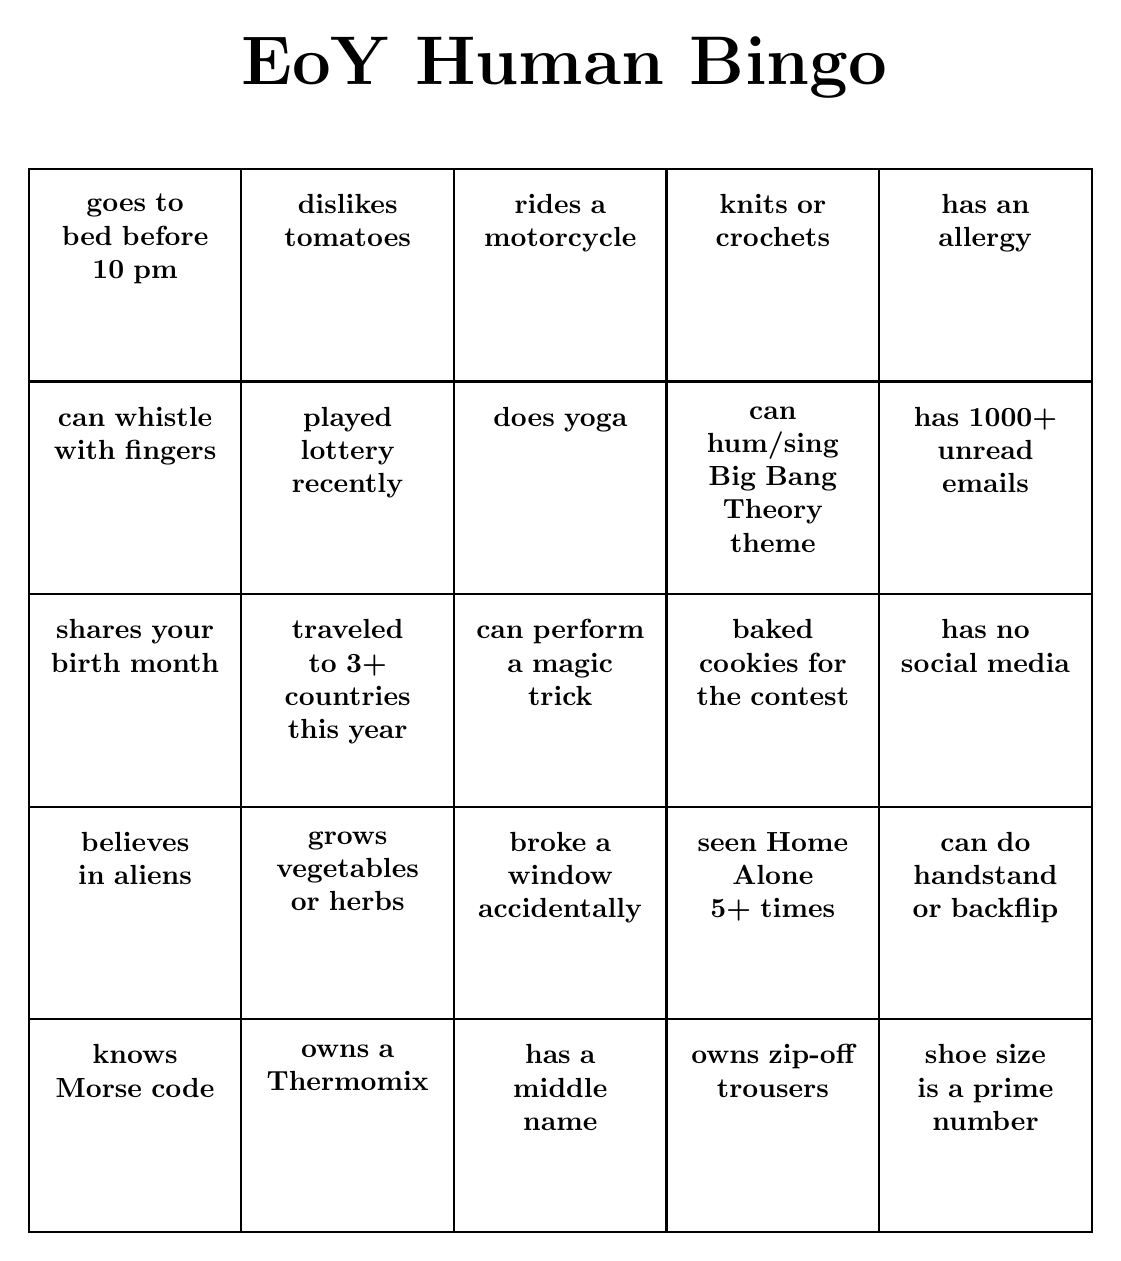
\begin{tikzpicture}
% Set the grid dimensions
\def\cellsize{2.7cm} % Each cell will be 2x2 cm

% Draw the grid and insert the numbers
\draw[thick] (0.0, 0.0) rectangle +(2.7, 2.7);
\node[anchor=north, align=center, text width=2.2cm] at (1.35, 2.5) {\textbf{goes to bed before 10 pm}};
\draw[thick] (2.7, 0.0) rectangle +(2.7, 2.7);
\node[anchor=north, align=center, text width=2.2cm] at (4.050000000000001, 2.5) {\textbf{dislikes tomatoes}};
\draw[thick] (5.4, 0.0) rectangle +(2.7, 2.7);
\node[anchor=north, align=center, text width=2.2cm] at (6.75, 2.5) {\textbf{rides a motorcycle}};
\draw[thick] (8.100000000000001, 0.0) rectangle +(2.7, 2.7);
\node[anchor=north, align=center, text width=2.2cm] at (9.450000000000001, 2.5) {\textbf{knits or crochets}};
\draw[thick] (10.8, 0.0) rectangle +(2.7, 2.7);
\node[anchor=north, align=center, text width=2.2cm] at (12.15, 2.5) {\textbf{has an allergy}};
\draw[thick] (0.0, -2.7) rectangle +(2.7, 2.7);
\node[anchor=north, align=center, text width=2.2cm] at (1.35, -0.2) {\textbf{can whistle with fingers}};
\draw[thick] (2.7, -2.7) rectangle +(2.7, 2.7);
\node[anchor=north, align=center, text width=2.2cm] at (4.050000000000001, -0.2) {\textbf{played lottery recently}};
\draw[thick] (5.4, -2.7) rectangle +(2.7, 2.7);
\node[anchor=north, align=center, text width=2.2cm] at (6.75, -0.2) {\textbf{does yoga}};
\draw[thick] (8.100000000000001, -2.7) rectangle +(2.7, 2.7);
\node[anchor=north, align=center, text width=2.2cm] at (9.450000000000001, -0.2) {\textbf{can hum/sing Big Bang Theory theme}};
\draw[thick] (10.8, -2.7) rectangle +(2.7, 2.7);
\node[anchor=north, align=center, text width=2.2cm] at (12.15, -0.2) {\textbf{has 1000+ unread emails}};
\draw[thick] (0.0, -5.4) rectangle +(2.7, 2.7);
\node[anchor=north, align=center, text width=2.2cm] at (1.35, -2.9000000000000004) {\textbf{shares your birth month}};
\draw[thick] (2.7, -5.4) rectangle +(2.7, 2.7);
\node[anchor=north, align=center, text width=2.2cm] at (4.050000000000001, -2.9000000000000004) {\textbf{traveled to 3+ countries this year}};
\draw[thick] (5.4, -5.4) rectangle +(2.7, 2.7);
\node[anchor=north, align=center, text width=2.2cm] at (6.75, -2.9000000000000004) {\textbf{can perform a magic trick}};
\draw[thick] (8.100000000000001, -5.4) rectangle +(2.7, 2.7);
\node[anchor=north, align=center, text width=2.2cm] at (9.450000000000001, -2.9000000000000004) {\textbf{baked cookies for the contest}};
\draw[thick] (10.8, -5.4) rectangle +(2.7, 2.7);
\node[anchor=north, align=center, text width=2.2cm] at (12.15, -2.9000000000000004) {\textbf{has no social media}};
\draw[thick] (0.0, -8.100000000000001) rectangle +(2.7, 2.7);
\node[anchor=north, align=center, text width=2.2cm] at (1.35, -5.600000000000001) {\textbf{believes in aliens}};
\draw[thick] (2.7, -8.100000000000001) rectangle +(2.7, 2.7);
\node[anchor=north, align=center, text width=2.2cm] at (4.050000000000001, -5.600000000000001) {\textbf{grows vegetables or herbs}};
\draw[thick] (5.4, -8.100000000000001) rectangle +(2.7, 2.7);
\node[anchor=north, align=center, text width=2.2cm] at (6.75, -5.600000000000001) {\textbf{broke a window accidentally}};
\draw[thick] (8.100000000000001, -8.100000000000001) rectangle +(2.7, 2.7);
\node[anchor=north, align=center, text width=2.2cm] at (9.450000000000001, -5.600000000000001) {\textbf{seen Home Alone 5+ times}};
\draw[thick] (10.8, -8.100000000000001) rectangle +(2.7, 2.7);
\node[anchor=north, align=center, text width=2.2cm] at (12.15, -5.600000000000001) {\textbf{can do handstand or backflip}};
\draw[thick] (0.0, -10.8) rectangle +(2.7, 2.7);
\node[anchor=north, align=center, text width=2.2cm] at (1.35, -8.3) {\textbf{knows Morse code}};
\draw[thick] (2.7, -10.8) rectangle +(2.7, 2.7);
\node[anchor=north, align=center, text width=2.2cm] at (4.050000000000001, -8.3) {\textbf{owns a Thermomix}};
\draw[thick] (5.4, -10.8) rectangle +(2.7, 2.7);
\node[anchor=north, align=center, text width=2.2cm] at (6.75, -8.3) {\textbf{has a middle name}};
\draw[thick] (8.100000000000001, -10.8) rectangle +(2.7, 2.7);
\node[anchor=north, align=center, text width=2.2cm] at (9.450000000000001, -8.3) {\textbf{owns zip-off trousers}};
\draw[thick] (10.8, -10.8) rectangle +(2.7, 2.7);
\node[anchor=north, align=center, text width=2.2cm] at (12.15, -8.3) {\textbf{shoe size is a prime number}};
\node[anchor=north, font = \Huge] at (6.8, 4.5){\textbf{EoY Human Bingo}};
\end{tikzpicture}
\end{center}
\newpage\begin{center}
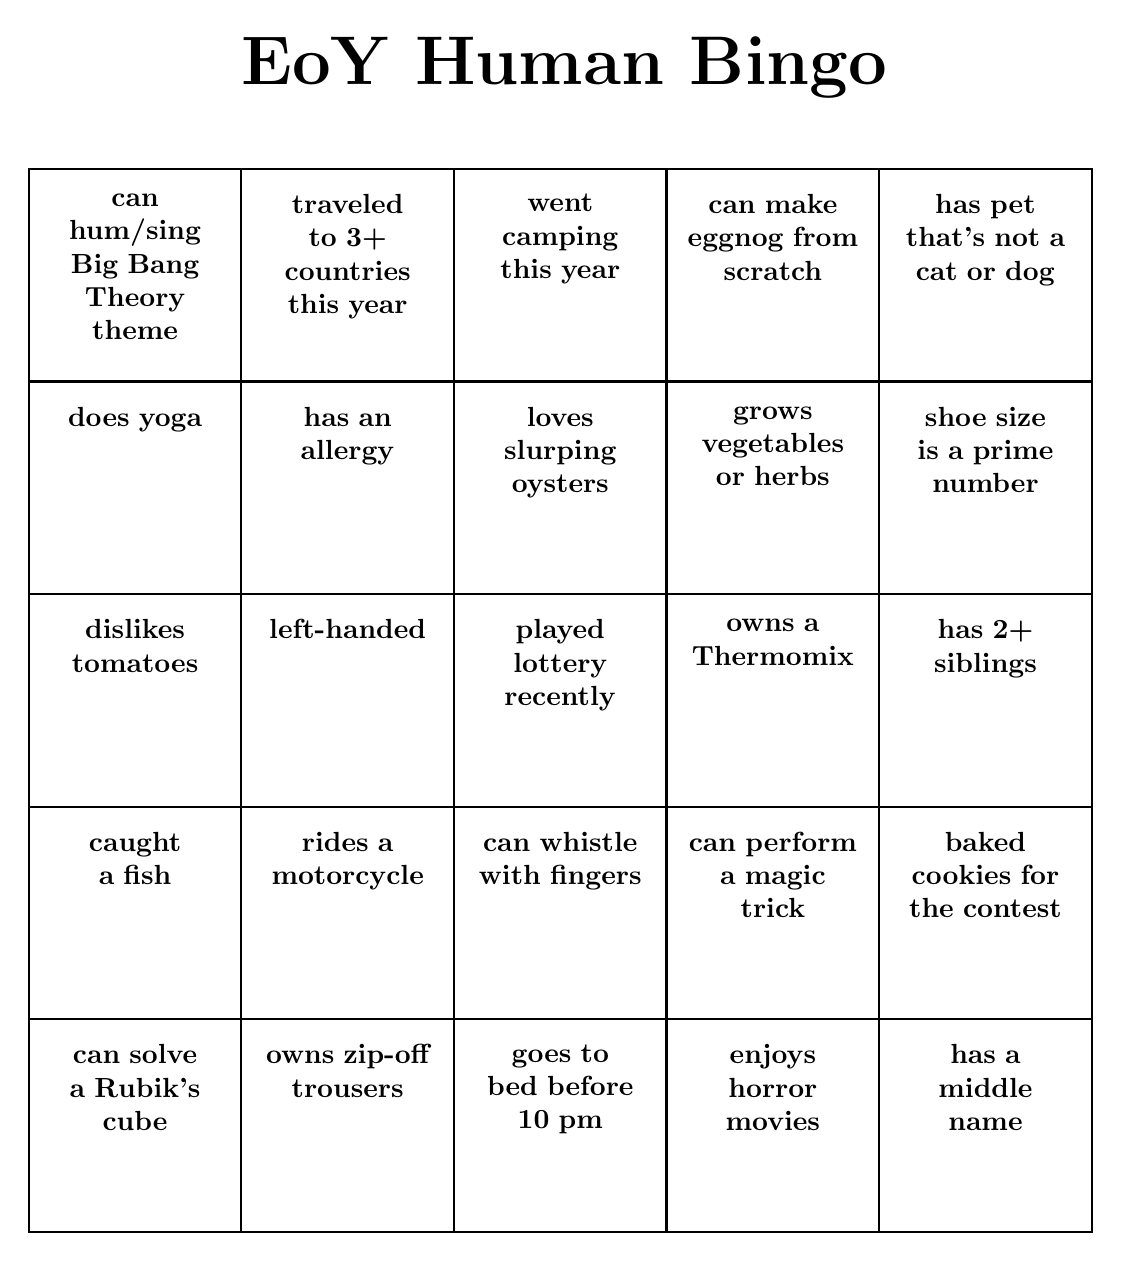
\begin{tikzpicture}
% Set the grid dimensions
\def\cellsize{2.7cm} % Each cell will be 2x2 cm

% Draw the grid and insert the numbers
\draw[thick] (0.0, 0.0) rectangle +(2.7, 2.7);
\node[anchor=north, align=center, text width=2.2cm] at (1.35, 2.5) {\textbf{can hum/sing Big Bang Theory theme}};
\draw[thick] (2.7, 0.0) rectangle +(2.7, 2.7);
\node[anchor=north, align=center, text width=2.2cm] at (4.050000000000001, 2.5) {\textbf{traveled to 3+ countries this year}};
\draw[thick] (5.4, 0.0) rectangle +(2.7, 2.7);
\node[anchor=north, align=center, text width=2.2cm] at (6.75, 2.5) {\textbf{went camping this year}};
\draw[thick] (8.100000000000001, 0.0) rectangle +(2.7, 2.7);
\node[anchor=north, align=center, text width=2.2cm] at (9.450000000000001, 2.5) {\textbf{can make eggnog from scratch}};
\draw[thick] (10.8, 0.0) rectangle +(2.7, 2.7);
\node[anchor=north, align=center, text width=2.2cm] at (12.15, 2.5) {\textbf{has pet that's not a cat or dog}};
\draw[thick] (0.0, -2.7) rectangle +(2.7, 2.7);
\node[anchor=north, align=center, text width=2.2cm] at (1.35, -0.2) {\textbf{does yoga}};
\draw[thick] (2.7, -2.7) rectangle +(2.7, 2.7);
\node[anchor=north, align=center, text width=2.2cm] at (4.050000000000001, -0.2) {\textbf{has an allergy}};
\draw[thick] (5.4, -2.7) rectangle +(2.7, 2.7);
\node[anchor=north, align=center, text width=2.2cm] at (6.75, -0.2) {\textbf{loves slurping oysters}};
\draw[thick] (8.100000000000001, -2.7) rectangle +(2.7, 2.7);
\node[anchor=north, align=center, text width=2.2cm] at (9.450000000000001, -0.2) {\textbf{grows vegetables or herbs}};
\draw[thick] (10.8, -2.7) rectangle +(2.7, 2.7);
\node[anchor=north, align=center, text width=2.2cm] at (12.15, -0.2) {\textbf{shoe size is a prime number}};
\draw[thick] (0.0, -5.4) rectangle +(2.7, 2.7);
\node[anchor=north, align=center, text width=2.2cm] at (1.35, -2.9000000000000004) {\textbf{dislikes tomatoes}};
\draw[thick] (2.7, -5.4) rectangle +(2.7, 2.7);
\node[anchor=north, align=center, text width=2.2cm] at (4.050000000000001, -2.9000000000000004) {\textbf{left-handed}};
\draw[thick] (5.4, -5.4) rectangle +(2.7, 2.7);
\node[anchor=north, align=center, text width=2.2cm] at (6.75, -2.9000000000000004) {\textbf{played lottery recently}};
\draw[thick] (8.100000000000001, -5.4) rectangle +(2.7, 2.7);
\node[anchor=north, align=center, text width=2.2cm] at (9.450000000000001, -2.9000000000000004) {\textbf{owns a Thermomix}};
\draw[thick] (10.8, -5.4) rectangle +(2.7, 2.7);
\node[anchor=north, align=center, text width=2.2cm] at (12.15, -2.9000000000000004) {\textbf{has 2+ siblings}};
\draw[thick] (0.0, -8.100000000000001) rectangle +(2.7, 2.7);
\node[anchor=north, align=center, text width=2.2cm] at (1.35, -5.600000000000001) {\textbf{caught a fish}};
\draw[thick] (2.7, -8.100000000000001) rectangle +(2.7, 2.7);
\node[anchor=north, align=center, text width=2.2cm] at (4.050000000000001, -5.600000000000001) {\textbf{rides a motorcycle}};
\draw[thick] (5.4, -8.100000000000001) rectangle +(2.7, 2.7);
\node[anchor=north, align=center, text width=2.2cm] at (6.75, -5.600000000000001) {\textbf{can whistle with fingers}};
\draw[thick] (8.100000000000001, -8.100000000000001) rectangle +(2.7, 2.7);
\node[anchor=north, align=center, text width=2.2cm] at (9.450000000000001, -5.600000000000001) {\textbf{can perform a magic trick}};
\draw[thick] (10.8, -8.100000000000001) rectangle +(2.7, 2.7);
\node[anchor=north, align=center, text width=2.2cm] at (12.15, -5.600000000000001) {\textbf{baked cookies for the contest}};
\draw[thick] (0.0, -10.8) rectangle +(2.7, 2.7);
\node[anchor=north, align=center, text width=2.2cm] at (1.35, -8.3) {\textbf{can solve a Rubik's cube}};
\draw[thick] (2.7, -10.8) rectangle +(2.7, 2.7);
\node[anchor=north, align=center, text width=2.2cm] at (4.050000000000001, -8.3) {\textbf{owns zip-off trousers}};
\draw[thick] (5.4, -10.8) rectangle +(2.7, 2.7);
\node[anchor=north, align=center, text width=2.2cm] at (6.75, -8.3) {\textbf{goes to bed before 10 pm}};
\draw[thick] (8.100000000000001, -10.8) rectangle +(2.7, 2.7);
\node[anchor=north, align=center, text width=2.2cm] at (9.450000000000001, -8.3) {\textbf{enjoys horror movies}};
\draw[thick] (10.8, -10.8) rectangle +(2.7, 2.7);
\node[anchor=north, align=center, text width=2.2cm] at (12.15, -8.3) {\textbf{has a middle name}};
\node[anchor=north, font = \Huge] at (6.8, 4.5){\textbf{EoY Human Bingo}};
\end{tikzpicture}
\end{center}
\newpage\begin{center}
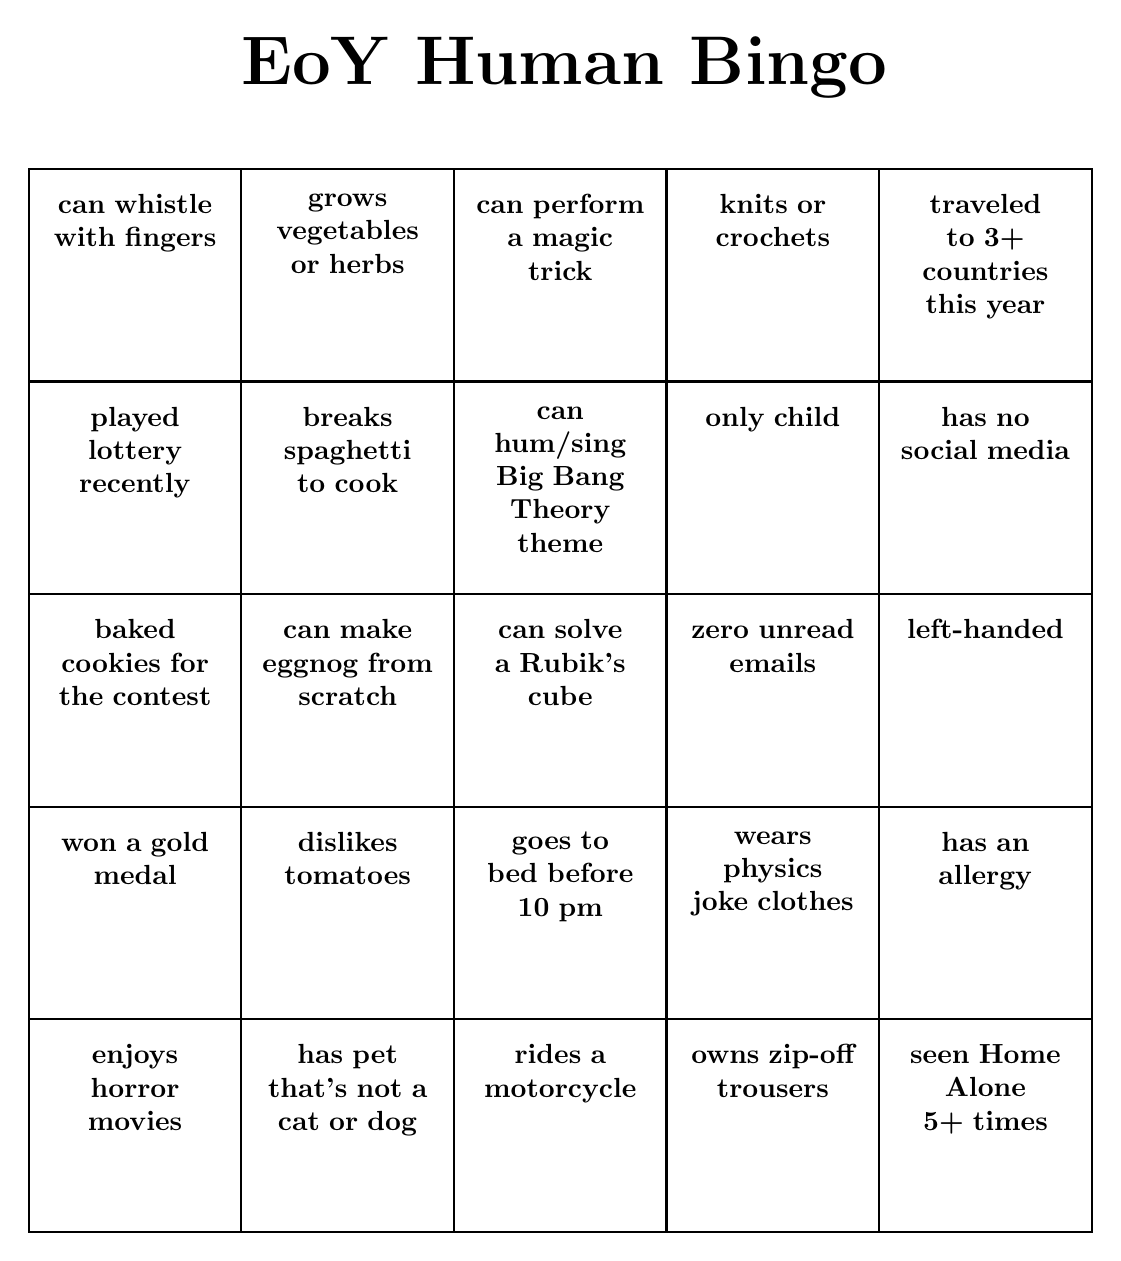
\begin{tikzpicture}
% Set the grid dimensions
\def\cellsize{2.7cm} % Each cell will be 2x2 cm

% Draw the grid and insert the numbers
\draw[thick] (0.0, 0.0) rectangle +(2.7, 2.7);
\node[anchor=north, align=center, text width=2.2cm] at (1.35, 2.5) {\textbf{can whistle with fingers}};
\draw[thick] (2.7, 0.0) rectangle +(2.7, 2.7);
\node[anchor=north, align=center, text width=2.2cm] at (4.050000000000001, 2.5) {\textbf{grows vegetables or herbs}};
\draw[thick] (5.4, 0.0) rectangle +(2.7, 2.7);
\node[anchor=north, align=center, text width=2.2cm] at (6.75, 2.5) {\textbf{can perform a magic trick}};
\draw[thick] (8.100000000000001, 0.0) rectangle +(2.7, 2.7);
\node[anchor=north, align=center, text width=2.2cm] at (9.450000000000001, 2.5) {\textbf{knits or crochets}};
\draw[thick] (10.8, 0.0) rectangle +(2.7, 2.7);
\node[anchor=north, align=center, text width=2.2cm] at (12.15, 2.5) {\textbf{traveled to 3+ countries this year}};
\draw[thick] (0.0, -2.7) rectangle +(2.7, 2.7);
\node[anchor=north, align=center, text width=2.2cm] at (1.35, -0.2) {\textbf{played lottery recently}};
\draw[thick] (2.7, -2.7) rectangle +(2.7, 2.7);
\node[anchor=north, align=center, text width=2.2cm] at (4.050000000000001, -0.2) {\textbf{breaks spaghetti to cook}};
\draw[thick] (5.4, -2.7) rectangle +(2.7, 2.7);
\node[anchor=north, align=center, text width=2.2cm] at (6.75, -0.2) {\textbf{can hum/sing Big Bang Theory theme}};
\draw[thick] (8.100000000000001, -2.7) rectangle +(2.7, 2.7);
\node[anchor=north, align=center, text width=2.2cm] at (9.450000000000001, -0.2) {\textbf{only child}};
\draw[thick] (10.8, -2.7) rectangle +(2.7, 2.7);
\node[anchor=north, align=center, text width=2.2cm] at (12.15, -0.2) {\textbf{has no social media}};
\draw[thick] (0.0, -5.4) rectangle +(2.7, 2.7);
\node[anchor=north, align=center, text width=2.2cm] at (1.35, -2.9000000000000004) {\textbf{baked cookies for the contest}};
\draw[thick] (2.7, -5.4) rectangle +(2.7, 2.7);
\node[anchor=north, align=center, text width=2.2cm] at (4.050000000000001, -2.9000000000000004) {\textbf{can make eggnog from scratch}};
\draw[thick] (5.4, -5.4) rectangle +(2.7, 2.7);
\node[anchor=north, align=center, text width=2.2cm] at (6.75, -2.9000000000000004) {\textbf{can solve a Rubik's cube}};
\draw[thick] (8.100000000000001, -5.4) rectangle +(2.7, 2.7);
\node[anchor=north, align=center, text width=2.2cm] at (9.450000000000001, -2.9000000000000004) {\textbf{zero unread emails}};
\draw[thick] (10.8, -5.4) rectangle +(2.7, 2.7);
\node[anchor=north, align=center, text width=2.2cm] at (12.15, -2.9000000000000004) {\textbf{left-handed}};
\draw[thick] (0.0, -8.100000000000001) rectangle +(2.7, 2.7);
\node[anchor=north, align=center, text width=2.2cm] at (1.35, -5.600000000000001) {\textbf{won a gold medal}};
\draw[thick] (2.7, -8.100000000000001) rectangle +(2.7, 2.7);
\node[anchor=north, align=center, text width=2.2cm] at (4.050000000000001, -5.600000000000001) {\textbf{dislikes tomatoes}};
\draw[thick] (5.4, -8.100000000000001) rectangle +(2.7, 2.7);
\node[anchor=north, align=center, text width=2.2cm] at (6.75, -5.600000000000001) {\textbf{goes to bed before 10 pm}};
\draw[thick] (8.100000000000001, -8.100000000000001) rectangle +(2.7, 2.7);
\node[anchor=north, align=center, text width=2.2cm] at (9.450000000000001, -5.600000000000001) {\textbf{wears physics joke clothes}};
\draw[thick] (10.8, -8.100000000000001) rectangle +(2.7, 2.7);
\node[anchor=north, align=center, text width=2.2cm] at (12.15, -5.600000000000001) {\textbf{has an allergy}};
\draw[thick] (0.0, -10.8) rectangle +(2.7, 2.7);
\node[anchor=north, align=center, text width=2.2cm] at (1.35, -8.3) {\textbf{enjoys horror movies}};
\draw[thick] (2.7, -10.8) rectangle +(2.7, 2.7);
\node[anchor=north, align=center, text width=2.2cm] at (4.050000000000001, -8.3) {\textbf{has pet that's not a cat or dog}};
\draw[thick] (5.4, -10.8) rectangle +(2.7, 2.7);
\node[anchor=north, align=center, text width=2.2cm] at (6.75, -8.3) {\textbf{rides a motorcycle}};
\draw[thick] (8.100000000000001, -10.8) rectangle +(2.7, 2.7);
\node[anchor=north, align=center, text width=2.2cm] at (9.450000000000001, -8.3) {\textbf{owns zip-off trousers}};
\draw[thick] (10.8, -10.8) rectangle +(2.7, 2.7);
\node[anchor=north, align=center, text width=2.2cm] at (12.15, -8.3) {\textbf{seen Home Alone 5+ times}};
\node[anchor=north, font = \Huge] at (6.8, 4.5){\textbf{EoY Human Bingo}};
\end{tikzpicture}
\end{center}
\newpage\begin{center}
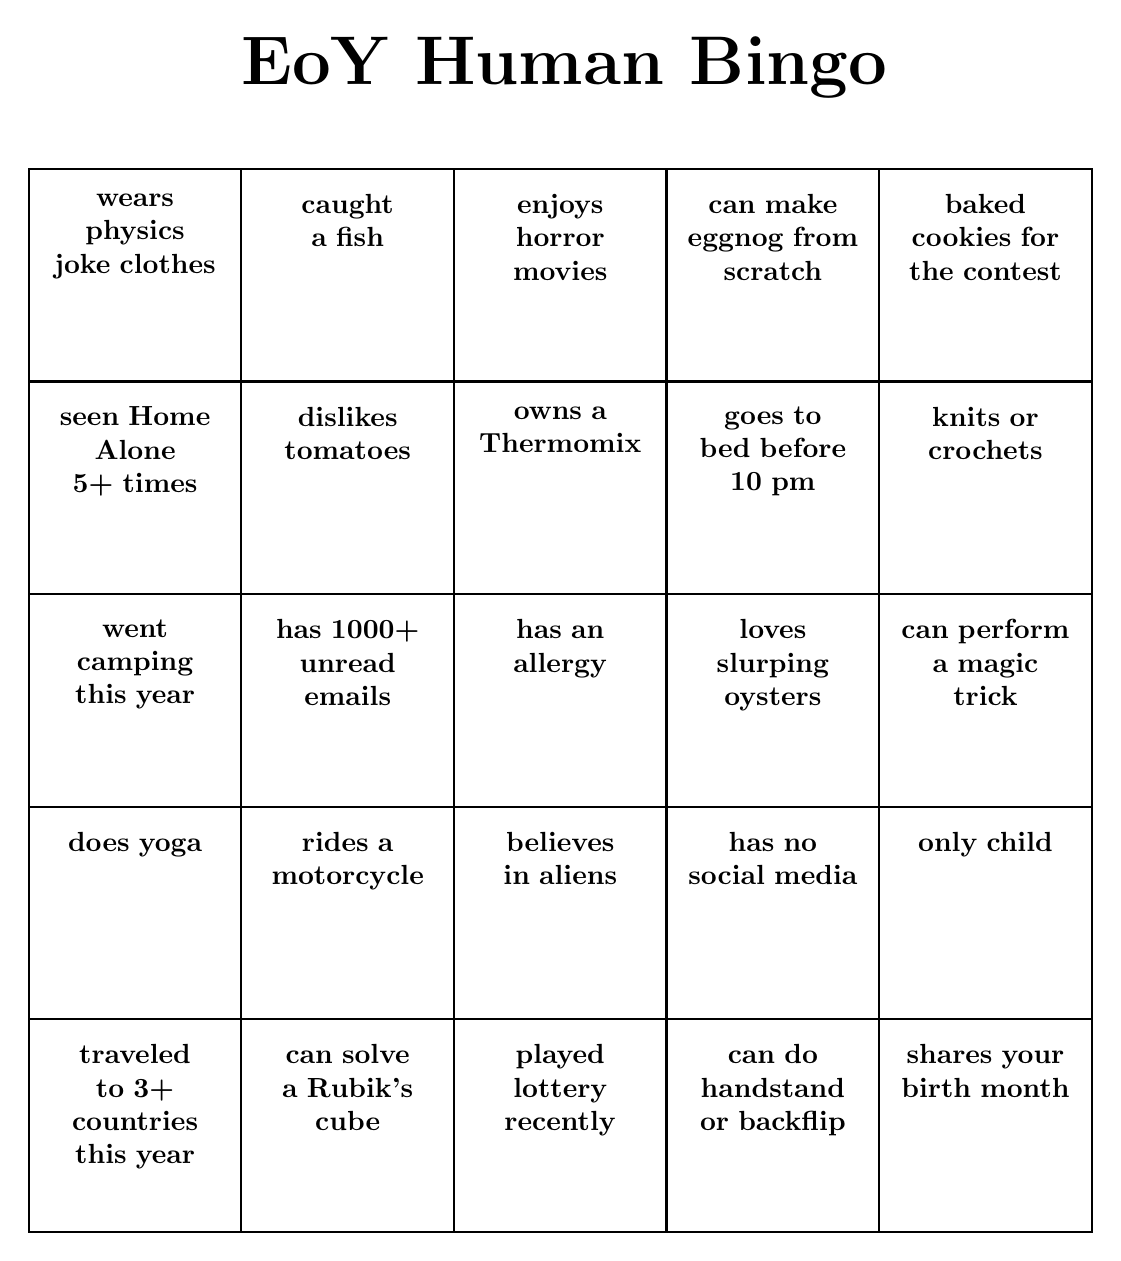
\begin{tikzpicture}
% Set the grid dimensions
\def\cellsize{2.7cm} % Each cell will be 2x2 cm

% Draw the grid and insert the numbers
\draw[thick] (0.0, 0.0) rectangle +(2.7, 2.7);
\node[anchor=north, align=center, text width=2.2cm] at (1.35, 2.5) {\textbf{wears physics joke clothes}};
\draw[thick] (2.7, 0.0) rectangle +(2.7, 2.7);
\node[anchor=north, align=center, text width=2.2cm] at (4.050000000000001, 2.5) {\textbf{caught a fish}};
\draw[thick] (5.4, 0.0) rectangle +(2.7, 2.7);
\node[anchor=north, align=center, text width=2.2cm] at (6.75, 2.5) {\textbf{enjoys horror movies}};
\draw[thick] (8.100000000000001, 0.0) rectangle +(2.7, 2.7);
\node[anchor=north, align=center, text width=2.2cm] at (9.450000000000001, 2.5) {\textbf{can make eggnog from scratch}};
\draw[thick] (10.8, 0.0) rectangle +(2.7, 2.7);
\node[anchor=north, align=center, text width=2.2cm] at (12.15, 2.5) {\textbf{baked cookies for the contest}};
\draw[thick] (0.0, -2.7) rectangle +(2.7, 2.7);
\node[anchor=north, align=center, text width=2.2cm] at (1.35, -0.2) {\textbf{seen Home Alone 5+ times}};
\draw[thick] (2.7, -2.7) rectangle +(2.7, 2.7);
\node[anchor=north, align=center, text width=2.2cm] at (4.050000000000001, -0.2) {\textbf{dislikes tomatoes}};
\draw[thick] (5.4, -2.7) rectangle +(2.7, 2.7);
\node[anchor=north, align=center, text width=2.2cm] at (6.75, -0.2) {\textbf{owns a Thermomix}};
\draw[thick] (8.100000000000001, -2.7) rectangle +(2.7, 2.7);
\node[anchor=north, align=center, text width=2.2cm] at (9.450000000000001, -0.2) {\textbf{goes to bed before 10 pm}};
\draw[thick] (10.8, -2.7) rectangle +(2.7, 2.7);
\node[anchor=north, align=center, text width=2.2cm] at (12.15, -0.2) {\textbf{knits or crochets}};
\draw[thick] (0.0, -5.4) rectangle +(2.7, 2.7);
\node[anchor=north, align=center, text width=2.2cm] at (1.35, -2.9000000000000004) {\textbf{went camping this year}};
\draw[thick] (2.7, -5.4) rectangle +(2.7, 2.7);
\node[anchor=north, align=center, text width=2.2cm] at (4.050000000000001, -2.9000000000000004) {\textbf{has 1000+ unread emails}};
\draw[thick] (5.4, -5.4) rectangle +(2.7, 2.7);
\node[anchor=north, align=center, text width=2.2cm] at (6.75, -2.9000000000000004) {\textbf{has an allergy}};
\draw[thick] (8.100000000000001, -5.4) rectangle +(2.7, 2.7);
\node[anchor=north, align=center, text width=2.2cm] at (9.450000000000001, -2.9000000000000004) {\textbf{loves slurping oysters}};
\draw[thick] (10.8, -5.4) rectangle +(2.7, 2.7);
\node[anchor=north, align=center, text width=2.2cm] at (12.15, -2.9000000000000004) {\textbf{can perform a magic trick}};
\draw[thick] (0.0, -8.100000000000001) rectangle +(2.7, 2.7);
\node[anchor=north, align=center, text width=2.2cm] at (1.35, -5.600000000000001) {\textbf{does yoga}};
\draw[thick] (2.7, -8.100000000000001) rectangle +(2.7, 2.7);
\node[anchor=north, align=center, text width=2.2cm] at (4.050000000000001, -5.600000000000001) {\textbf{rides a motorcycle}};
\draw[thick] (5.4, -8.100000000000001) rectangle +(2.7, 2.7);
\node[anchor=north, align=center, text width=2.2cm] at (6.75, -5.600000000000001) {\textbf{believes in aliens}};
\draw[thick] (8.100000000000001, -8.100000000000001) rectangle +(2.7, 2.7);
\node[anchor=north, align=center, text width=2.2cm] at (9.450000000000001, -5.600000000000001) {\textbf{has no social media}};
\draw[thick] (10.8, -8.100000000000001) rectangle +(2.7, 2.7);
\node[anchor=north, align=center, text width=2.2cm] at (12.15, -5.600000000000001) {\textbf{only child}};
\draw[thick] (0.0, -10.8) rectangle +(2.7, 2.7);
\node[anchor=north, align=center, text width=2.2cm] at (1.35, -8.3) {\textbf{traveled to 3+ countries this year}};
\draw[thick] (2.7, -10.8) rectangle +(2.7, 2.7);
\node[anchor=north, align=center, text width=2.2cm] at (4.050000000000001, -8.3) {\textbf{can solve a Rubik's cube}};
\draw[thick] (5.4, -10.8) rectangle +(2.7, 2.7);
\node[anchor=north, align=center, text width=2.2cm] at (6.75, -8.3) {\textbf{played lottery recently}};
\draw[thick] (8.100000000000001, -10.8) rectangle +(2.7, 2.7);
\node[anchor=north, align=center, text width=2.2cm] at (9.450000000000001, -8.3) {\textbf{can do handstand or backflip}};
\draw[thick] (10.8, -10.8) rectangle +(2.7, 2.7);
\node[anchor=north, align=center, text width=2.2cm] at (12.15, -8.3) {\textbf{shares your birth month}};
\node[anchor=north, font = \Huge] at (6.8, 4.5){\textbf{EoY Human Bingo}};
\end{tikzpicture}
\end{center}
\newpage\begin{center}
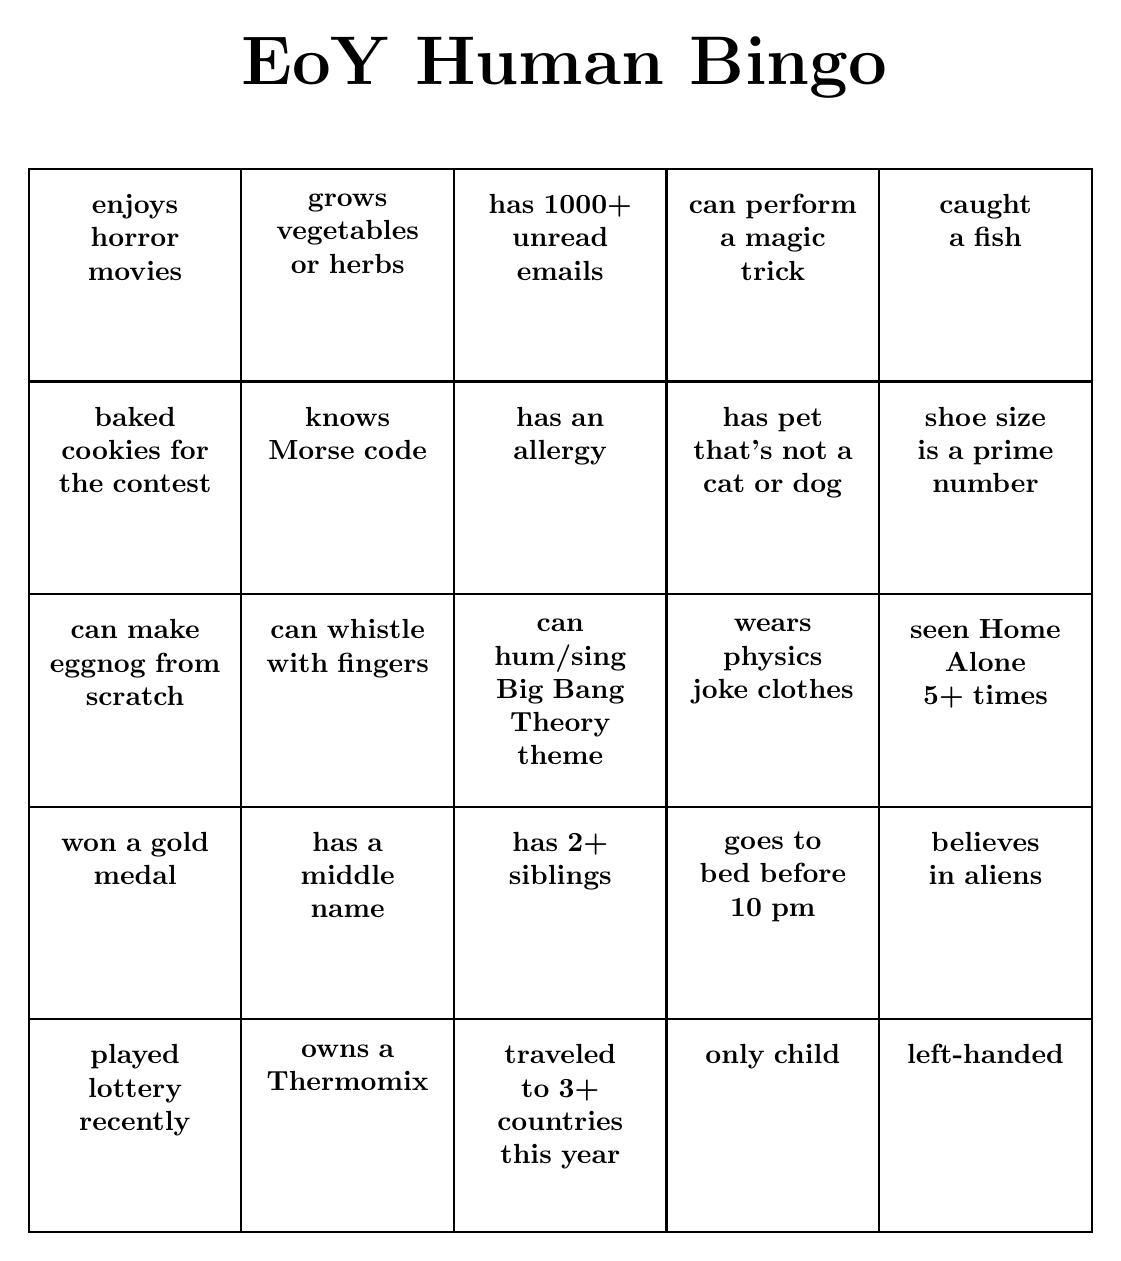
\begin{tikzpicture}
% Set the grid dimensions
\def\cellsize{2.7cm} % Each cell will be 2x2 cm

% Draw the grid and insert the numbers
\draw[thick] (0.0, 0.0) rectangle +(2.7, 2.7);
\node[anchor=north, align=center, text width=2.2cm] at (1.35, 2.5) {\textbf{enjoys horror movies}};
\draw[thick] (2.7, 0.0) rectangle +(2.7, 2.7);
\node[anchor=north, align=center, text width=2.2cm] at (4.050000000000001, 2.5) {\textbf{grows vegetables or herbs}};
\draw[thick] (5.4, 0.0) rectangle +(2.7, 2.7);
\node[anchor=north, align=center, text width=2.2cm] at (6.75, 2.5) {\textbf{has 1000+ unread emails}};
\draw[thick] (8.100000000000001, 0.0) rectangle +(2.7, 2.7);
\node[anchor=north, align=center, text width=2.2cm] at (9.450000000000001, 2.5) {\textbf{can perform a magic trick}};
\draw[thick] (10.8, 0.0) rectangle +(2.7, 2.7);
\node[anchor=north, align=center, text width=2.2cm] at (12.15, 2.5) {\textbf{caught a fish}};
\draw[thick] (0.0, -2.7) rectangle +(2.7, 2.7);
\node[anchor=north, align=center, text width=2.2cm] at (1.35, -0.2) {\textbf{baked cookies for the contest}};
\draw[thick] (2.7, -2.7) rectangle +(2.7, 2.7);
\node[anchor=north, align=center, text width=2.2cm] at (4.050000000000001, -0.2) {\textbf{knows Morse code}};
\draw[thick] (5.4, -2.7) rectangle +(2.7, 2.7);
\node[anchor=north, align=center, text width=2.2cm] at (6.75, -0.2) {\textbf{has an allergy}};
\draw[thick] (8.100000000000001, -2.7) rectangle +(2.7, 2.7);
\node[anchor=north, align=center, text width=2.2cm] at (9.450000000000001, -0.2) {\textbf{has pet that's not a cat or dog}};
\draw[thick] (10.8, -2.7) rectangle +(2.7, 2.7);
\node[anchor=north, align=center, text width=2.2cm] at (12.15, -0.2) {\textbf{shoe size is a prime number}};
\draw[thick] (0.0, -5.4) rectangle +(2.7, 2.7);
\node[anchor=north, align=center, text width=2.2cm] at (1.35, -2.9000000000000004) {\textbf{can make eggnog from scratch}};
\draw[thick] (2.7, -5.4) rectangle +(2.7, 2.7);
\node[anchor=north, align=center, text width=2.2cm] at (4.050000000000001, -2.9000000000000004) {\textbf{can whistle with fingers}};
\draw[thick] (5.4, -5.4) rectangle +(2.7, 2.7);
\node[anchor=north, align=center, text width=2.2cm] at (6.75, -2.9000000000000004) {\textbf{can hum/sing Big Bang Theory theme}};
\draw[thick] (8.100000000000001, -5.4) rectangle +(2.7, 2.7);
\node[anchor=north, align=center, text width=2.2cm] at (9.450000000000001, -2.9000000000000004) {\textbf{wears physics joke clothes}};
\draw[thick] (10.8, -5.4) rectangle +(2.7, 2.7);
\node[anchor=north, align=center, text width=2.2cm] at (12.15, -2.9000000000000004) {\textbf{seen Home Alone 5+ times}};
\draw[thick] (0.0, -8.100000000000001) rectangle +(2.7, 2.7);
\node[anchor=north, align=center, text width=2.2cm] at (1.35, -5.600000000000001) {\textbf{won a gold medal}};
\draw[thick] (2.7, -8.100000000000001) rectangle +(2.7, 2.7);
\node[anchor=north, align=center, text width=2.2cm] at (4.050000000000001, -5.600000000000001) {\textbf{has a middle name}};
\draw[thick] (5.4, -8.100000000000001) rectangle +(2.7, 2.7);
\node[anchor=north, align=center, text width=2.2cm] at (6.75, -5.600000000000001) {\textbf{has 2+ siblings}};
\draw[thick] (8.100000000000001, -8.100000000000001) rectangle +(2.7, 2.7);
\node[anchor=north, align=center, text width=2.2cm] at (9.450000000000001, -5.600000000000001) {\textbf{goes to bed before 10 pm}};
\draw[thick] (10.8, -8.100000000000001) rectangle +(2.7, 2.7);
\node[anchor=north, align=center, text width=2.2cm] at (12.15, -5.600000000000001) {\textbf{believes in aliens}};
\draw[thick] (0.0, -10.8) rectangle +(2.7, 2.7);
\node[anchor=north, align=center, text width=2.2cm] at (1.35, -8.3) {\textbf{played lottery recently}};
\draw[thick] (2.7, -10.8) rectangle +(2.7, 2.7);
\node[anchor=north, align=center, text width=2.2cm] at (4.050000000000001, -8.3) {\textbf{owns a Thermomix}};
\draw[thick] (5.4, -10.8) rectangle +(2.7, 2.7);
\node[anchor=north, align=center, text width=2.2cm] at (6.75, -8.3) {\textbf{traveled to 3+ countries this year}};
\draw[thick] (8.100000000000001, -10.8) rectangle +(2.7, 2.7);
\node[anchor=north, align=center, text width=2.2cm] at (9.450000000000001, -8.3) {\textbf{only child}};
\draw[thick] (10.8, -10.8) rectangle +(2.7, 2.7);
\node[anchor=north, align=center, text width=2.2cm] at (12.15, -8.3) {\textbf{left-handed}};
\node[anchor=north, font = \Huge] at (6.8, 4.5){\textbf{EoY Human Bingo}};
\end{tikzpicture}
\end{center}
\newpage\begin{center}
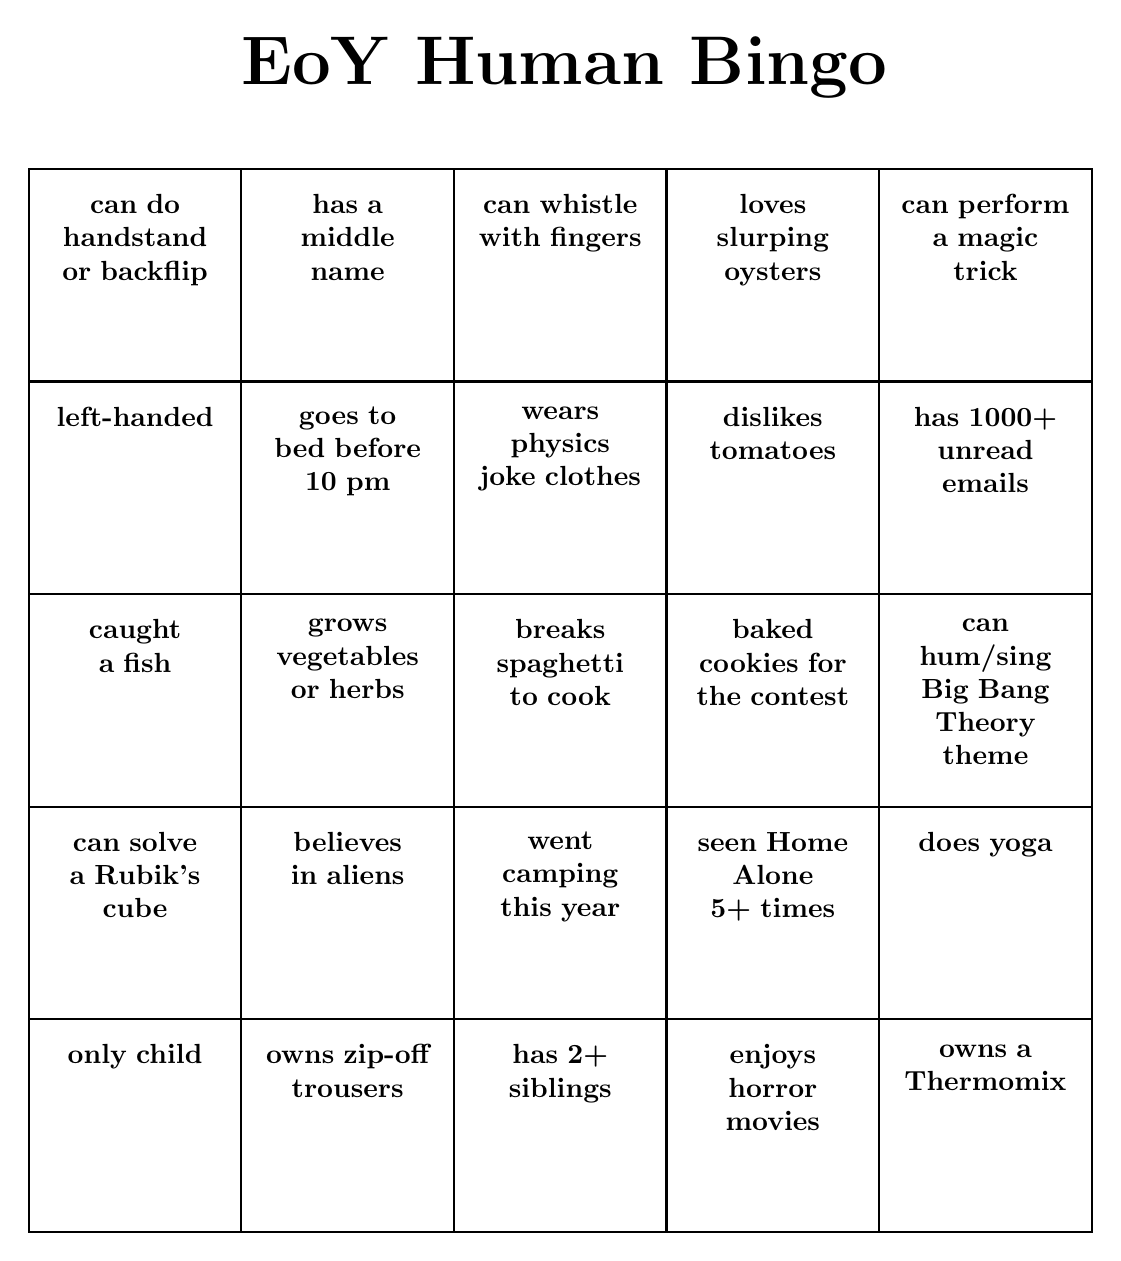
\begin{tikzpicture}
% Set the grid dimensions
\def\cellsize{2.7cm} % Each cell will be 2x2 cm

% Draw the grid and insert the numbers
\draw[thick] (0.0, 0.0) rectangle +(2.7, 2.7);
\node[anchor=north, align=center, text width=2.2cm] at (1.35, 2.5) {\textbf{can do handstand or backflip}};
\draw[thick] (2.7, 0.0) rectangle +(2.7, 2.7);
\node[anchor=north, align=center, text width=2.2cm] at (4.050000000000001, 2.5) {\textbf{has a middle name}};
\draw[thick] (5.4, 0.0) rectangle +(2.7, 2.7);
\node[anchor=north, align=center, text width=2.2cm] at (6.75, 2.5) {\textbf{can whistle with fingers}};
\draw[thick] (8.100000000000001, 0.0) rectangle +(2.7, 2.7);
\node[anchor=north, align=center, text width=2.2cm] at (9.450000000000001, 2.5) {\textbf{loves slurping oysters}};
\draw[thick] (10.8, 0.0) rectangle +(2.7, 2.7);
\node[anchor=north, align=center, text width=2.2cm] at (12.15, 2.5) {\textbf{can perform a magic trick}};
\draw[thick] (0.0, -2.7) rectangle +(2.7, 2.7);
\node[anchor=north, align=center, text width=2.2cm] at (1.35, -0.2) {\textbf{left-handed}};
\draw[thick] (2.7, -2.7) rectangle +(2.7, 2.7);
\node[anchor=north, align=center, text width=2.2cm] at (4.050000000000001, -0.2) {\textbf{goes to bed before 10 pm}};
\draw[thick] (5.4, -2.7) rectangle +(2.7, 2.7);
\node[anchor=north, align=center, text width=2.2cm] at (6.75, -0.2) {\textbf{wears physics joke clothes}};
\draw[thick] (8.100000000000001, -2.7) rectangle +(2.7, 2.7);
\node[anchor=north, align=center, text width=2.2cm] at (9.450000000000001, -0.2) {\textbf{dislikes tomatoes}};
\draw[thick] (10.8, -2.7) rectangle +(2.7, 2.7);
\node[anchor=north, align=center, text width=2.2cm] at (12.15, -0.2) {\textbf{has 1000+ unread emails}};
\draw[thick] (0.0, -5.4) rectangle +(2.7, 2.7);
\node[anchor=north, align=center, text width=2.2cm] at (1.35, -2.9000000000000004) {\textbf{caught a fish}};
\draw[thick] (2.7, -5.4) rectangle +(2.7, 2.7);
\node[anchor=north, align=center, text width=2.2cm] at (4.050000000000001, -2.9000000000000004) {\textbf{grows vegetables or herbs}};
\draw[thick] (5.4, -5.4) rectangle +(2.7, 2.7);
\node[anchor=north, align=center, text width=2.2cm] at (6.75, -2.9000000000000004) {\textbf{breaks spaghetti to cook}};
\draw[thick] (8.100000000000001, -5.4) rectangle +(2.7, 2.7);
\node[anchor=north, align=center, text width=2.2cm] at (9.450000000000001, -2.9000000000000004) {\textbf{baked cookies for the contest}};
\draw[thick] (10.8, -5.4) rectangle +(2.7, 2.7);
\node[anchor=north, align=center, text width=2.2cm] at (12.15, -2.9000000000000004) {\textbf{can hum/sing Big Bang Theory theme}};
\draw[thick] (0.0, -8.100000000000001) rectangle +(2.7, 2.7);
\node[anchor=north, align=center, text width=2.2cm] at (1.35, -5.600000000000001) {\textbf{can solve a Rubik's cube}};
\draw[thick] (2.7, -8.100000000000001) rectangle +(2.7, 2.7);
\node[anchor=north, align=center, text width=2.2cm] at (4.050000000000001, -5.600000000000001) {\textbf{believes in aliens}};
\draw[thick] (5.4, -8.100000000000001) rectangle +(2.7, 2.7);
\node[anchor=north, align=center, text width=2.2cm] at (6.75, -5.600000000000001) {\textbf{went camping this year}};
\draw[thick] (8.100000000000001, -8.100000000000001) rectangle +(2.7, 2.7);
\node[anchor=north, align=center, text width=2.2cm] at (9.450000000000001, -5.600000000000001) {\textbf{seen Home Alone 5+ times}};
\draw[thick] (10.8, -8.100000000000001) rectangle +(2.7, 2.7);
\node[anchor=north, align=center, text width=2.2cm] at (12.15, -5.600000000000001) {\textbf{does yoga}};
\draw[thick] (0.0, -10.8) rectangle +(2.7, 2.7);
\node[anchor=north, align=center, text width=2.2cm] at (1.35, -8.3) {\textbf{only child}};
\draw[thick] (2.7, -10.8) rectangle +(2.7, 2.7);
\node[anchor=north, align=center, text width=2.2cm] at (4.050000000000001, -8.3) {\textbf{owns zip-off trousers}};
\draw[thick] (5.4, -10.8) rectangle +(2.7, 2.7);
\node[anchor=north, align=center, text width=2.2cm] at (6.75, -8.3) {\textbf{has 2+ siblings}};
\draw[thick] (8.100000000000001, -10.8) rectangle +(2.7, 2.7);
\node[anchor=north, align=center, text width=2.2cm] at (9.450000000000001, -8.3) {\textbf{enjoys horror movies}};
\draw[thick] (10.8, -10.8) rectangle +(2.7, 2.7);
\node[anchor=north, align=center, text width=2.2cm] at (12.15, -8.3) {\textbf{owns a Thermomix}};
\node[anchor=north, font = \Huge] at (6.8, 4.5){\textbf{EoY Human Bingo}};
\end{tikzpicture}
\end{center}
\newpage\begin{center}
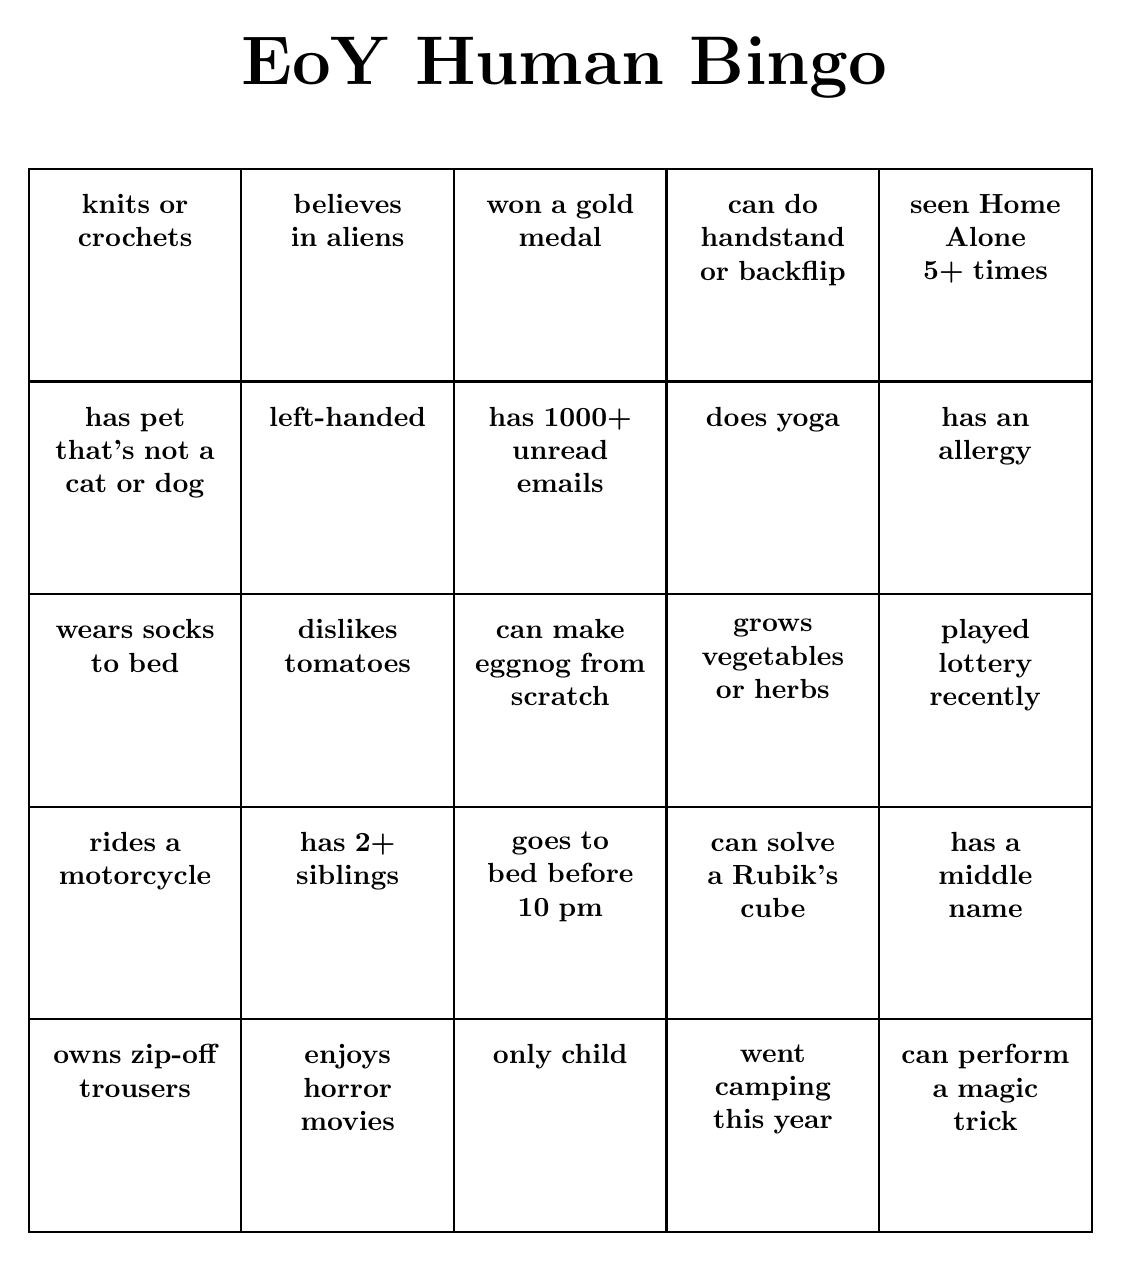
\begin{tikzpicture}
% Set the grid dimensions
\def\cellsize{2.7cm} % Each cell will be 2x2 cm

% Draw the grid and insert the numbers
\draw[thick] (0.0, 0.0) rectangle +(2.7, 2.7);
\node[anchor=north, align=center, text width=2.2cm] at (1.35, 2.5) {\textbf{knits or crochets}};
\draw[thick] (2.7, 0.0) rectangle +(2.7, 2.7);
\node[anchor=north, align=center, text width=2.2cm] at (4.050000000000001, 2.5) {\textbf{believes in aliens}};
\draw[thick] (5.4, 0.0) rectangle +(2.7, 2.7);
\node[anchor=north, align=center, text width=2.2cm] at (6.75, 2.5) {\textbf{won a gold medal}};
\draw[thick] (8.100000000000001, 0.0) rectangle +(2.7, 2.7);
\node[anchor=north, align=center, text width=2.2cm] at (9.450000000000001, 2.5) {\textbf{can do handstand or backflip}};
\draw[thick] (10.8, 0.0) rectangle +(2.7, 2.7);
\node[anchor=north, align=center, text width=2.2cm] at (12.15, 2.5) {\textbf{seen Home Alone 5+ times}};
\draw[thick] (0.0, -2.7) rectangle +(2.7, 2.7);
\node[anchor=north, align=center, text width=2.2cm] at (1.35, -0.2) {\textbf{has pet that's not a cat or dog}};
\draw[thick] (2.7, -2.7) rectangle +(2.7, 2.7);
\node[anchor=north, align=center, text width=2.2cm] at (4.050000000000001, -0.2) {\textbf{left-handed}};
\draw[thick] (5.4, -2.7) rectangle +(2.7, 2.7);
\node[anchor=north, align=center, text width=2.2cm] at (6.75, -0.2) {\textbf{has 1000+ unread emails}};
\draw[thick] (8.100000000000001, -2.7) rectangle +(2.7, 2.7);
\node[anchor=north, align=center, text width=2.2cm] at (9.450000000000001, -0.2) {\textbf{does yoga}};
\draw[thick] (10.8, -2.7) rectangle +(2.7, 2.7);
\node[anchor=north, align=center, text width=2.2cm] at (12.15, -0.2) {\textbf{has an allergy}};
\draw[thick] (0.0, -5.4) rectangle +(2.7, 2.7);
\node[anchor=north, align=center, text width=2.2cm] at (1.35, -2.9000000000000004) {\textbf{wears socks to bed}};
\draw[thick] (2.7, -5.4) rectangle +(2.7, 2.7);
\node[anchor=north, align=center, text width=2.2cm] at (4.050000000000001, -2.9000000000000004) {\textbf{dislikes tomatoes}};
\draw[thick] (5.4, -5.4) rectangle +(2.7, 2.7);
\node[anchor=north, align=center, text width=2.2cm] at (6.75, -2.9000000000000004) {\textbf{can make eggnog from scratch}};
\draw[thick] (8.100000000000001, -5.4) rectangle +(2.7, 2.7);
\node[anchor=north, align=center, text width=2.2cm] at (9.450000000000001, -2.9000000000000004) {\textbf{grows vegetables or herbs}};
\draw[thick] (10.8, -5.4) rectangle +(2.7, 2.7);
\node[anchor=north, align=center, text width=2.2cm] at (12.15, -2.9000000000000004) {\textbf{played lottery recently}};
\draw[thick] (0.0, -8.100000000000001) rectangle +(2.7, 2.7);
\node[anchor=north, align=center, text width=2.2cm] at (1.35, -5.600000000000001) {\textbf{rides a motorcycle}};
\draw[thick] (2.7, -8.100000000000001) rectangle +(2.7, 2.7);
\node[anchor=north, align=center, text width=2.2cm] at (4.050000000000001, -5.600000000000001) {\textbf{has 2+ siblings}};
\draw[thick] (5.4, -8.100000000000001) rectangle +(2.7, 2.7);
\node[anchor=north, align=center, text width=2.2cm] at (6.75, -5.600000000000001) {\textbf{goes to bed before 10 pm}};
\draw[thick] (8.100000000000001, -8.100000000000001) rectangle +(2.7, 2.7);
\node[anchor=north, align=center, text width=2.2cm] at (9.450000000000001, -5.600000000000001) {\textbf{can solve a Rubik's cube}};
\draw[thick] (10.8, -8.100000000000001) rectangle +(2.7, 2.7);
\node[anchor=north, align=center, text width=2.2cm] at (12.15, -5.600000000000001) {\textbf{has a middle name}};
\draw[thick] (0.0, -10.8) rectangle +(2.7, 2.7);
\node[anchor=north, align=center, text width=2.2cm] at (1.35, -8.3) {\textbf{owns zip-off trousers}};
\draw[thick] (2.7, -10.8) rectangle +(2.7, 2.7);
\node[anchor=north, align=center, text width=2.2cm] at (4.050000000000001, -8.3) {\textbf{enjoys horror movies}};
\draw[thick] (5.4, -10.8) rectangle +(2.7, 2.7);
\node[anchor=north, align=center, text width=2.2cm] at (6.75, -8.3) {\textbf{only child}};
\draw[thick] (8.100000000000001, -10.8) rectangle +(2.7, 2.7);
\node[anchor=north, align=center, text width=2.2cm] at (9.450000000000001, -8.3) {\textbf{went camping this year}};
\draw[thick] (10.8, -10.8) rectangle +(2.7, 2.7);
\node[anchor=north, align=center, text width=2.2cm] at (12.15, -8.3) {\textbf{can perform a magic trick}};
\node[anchor=north, font = \Huge] at (6.8, 4.5){\textbf{EoY Human Bingo}};
\end{tikzpicture}
\end{center}
\newpage\begin{center}
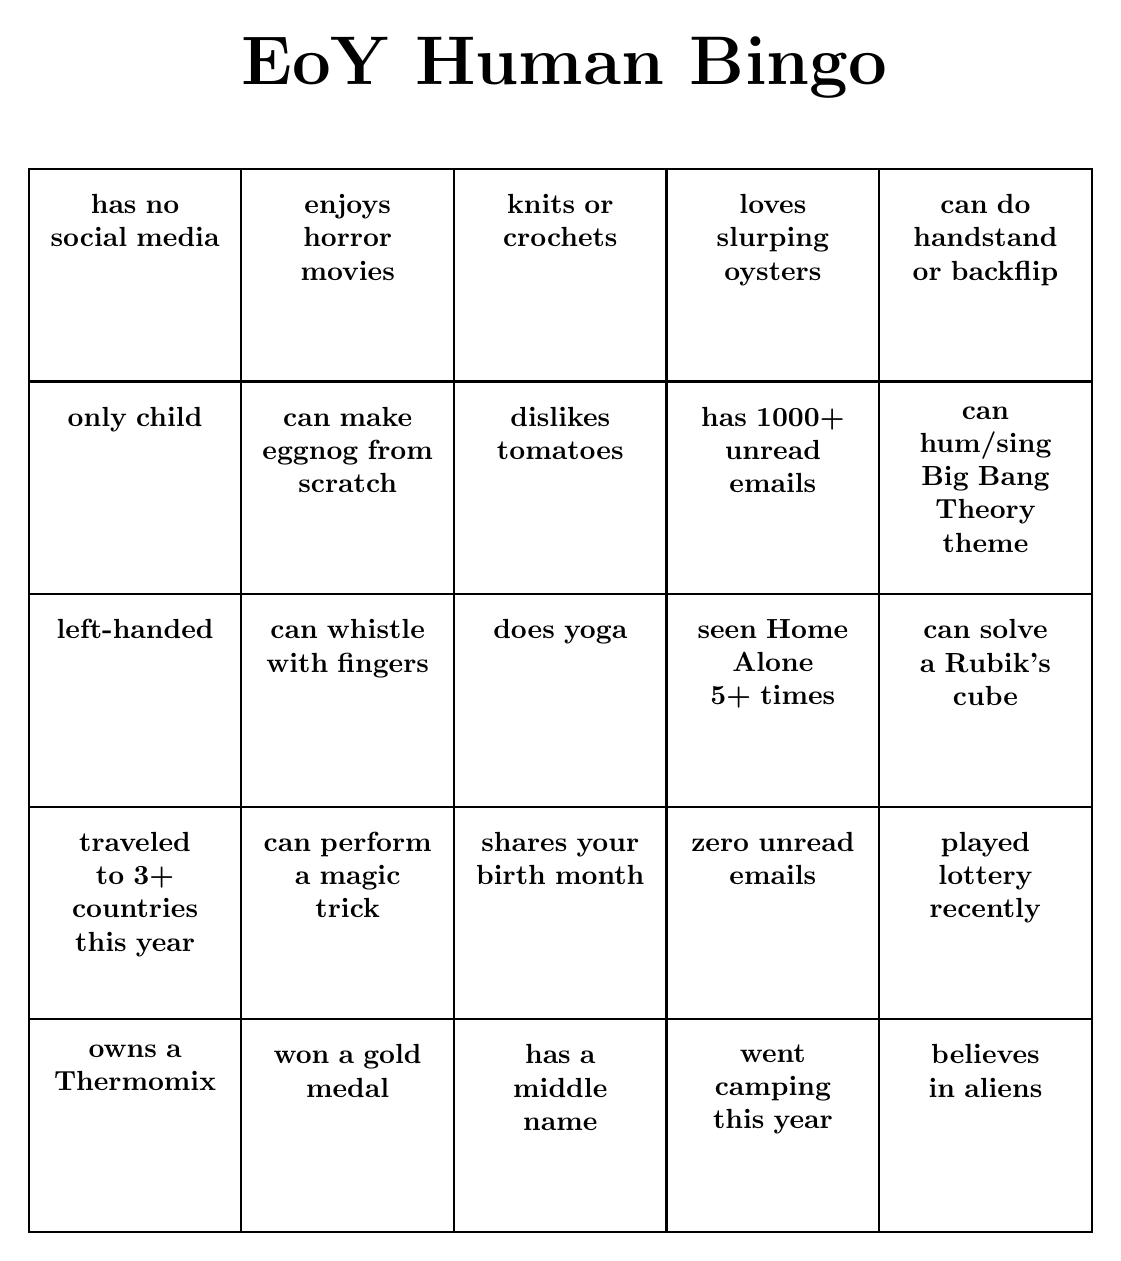
\begin{tikzpicture}
% Set the grid dimensions
\def\cellsize{2.7cm} % Each cell will be 2x2 cm

% Draw the grid and insert the numbers
\draw[thick] (0.0, 0.0) rectangle +(2.7, 2.7);
\node[anchor=north, align=center, text width=2.2cm] at (1.35, 2.5) {\textbf{has no social media}};
\draw[thick] (2.7, 0.0) rectangle +(2.7, 2.7);
\node[anchor=north, align=center, text width=2.2cm] at (4.050000000000001, 2.5) {\textbf{enjoys horror movies}};
\draw[thick] (5.4, 0.0) rectangle +(2.7, 2.7);
\node[anchor=north, align=center, text width=2.2cm] at (6.75, 2.5) {\textbf{knits or crochets}};
\draw[thick] (8.100000000000001, 0.0) rectangle +(2.7, 2.7);
\node[anchor=north, align=center, text width=2.2cm] at (9.450000000000001, 2.5) {\textbf{loves slurping oysters}};
\draw[thick] (10.8, 0.0) rectangle +(2.7, 2.7);
\node[anchor=north, align=center, text width=2.2cm] at (12.15, 2.5) {\textbf{can do handstand or backflip}};
\draw[thick] (0.0, -2.7) rectangle +(2.7, 2.7);
\node[anchor=north, align=center, text width=2.2cm] at (1.35, -0.2) {\textbf{only child}};
\draw[thick] (2.7, -2.7) rectangle +(2.7, 2.7);
\node[anchor=north, align=center, text width=2.2cm] at (4.050000000000001, -0.2) {\textbf{can make eggnog from scratch}};
\draw[thick] (5.4, -2.7) rectangle +(2.7, 2.7);
\node[anchor=north, align=center, text width=2.2cm] at (6.75, -0.2) {\textbf{dislikes tomatoes}};
\draw[thick] (8.100000000000001, -2.7) rectangle +(2.7, 2.7);
\node[anchor=north, align=center, text width=2.2cm] at (9.450000000000001, -0.2) {\textbf{has 1000+ unread emails}};
\draw[thick] (10.8, -2.7) rectangle +(2.7, 2.7);
\node[anchor=north, align=center, text width=2.2cm] at (12.15, -0.2) {\textbf{can hum/sing Big Bang Theory theme}};
\draw[thick] (0.0, -5.4) rectangle +(2.7, 2.7);
\node[anchor=north, align=center, text width=2.2cm] at (1.35, -2.9000000000000004) {\textbf{left-handed}};
\draw[thick] (2.7, -5.4) rectangle +(2.7, 2.7);
\node[anchor=north, align=center, text width=2.2cm] at (4.050000000000001, -2.9000000000000004) {\textbf{can whistle with fingers}};
\draw[thick] (5.4, -5.4) rectangle +(2.7, 2.7);
\node[anchor=north, align=center, text width=2.2cm] at (6.75, -2.9000000000000004) {\textbf{does yoga}};
\draw[thick] (8.100000000000001, -5.4) rectangle +(2.7, 2.7);
\node[anchor=north, align=center, text width=2.2cm] at (9.450000000000001, -2.9000000000000004) {\textbf{seen Home Alone 5+ times}};
\draw[thick] (10.8, -5.4) rectangle +(2.7, 2.7);
\node[anchor=north, align=center, text width=2.2cm] at (12.15, -2.9000000000000004) {\textbf{can solve a Rubik's cube}};
\draw[thick] (0.0, -8.100000000000001) rectangle +(2.7, 2.7);
\node[anchor=north, align=center, text width=2.2cm] at (1.35, -5.600000000000001) {\textbf{traveled to 3+ countries this year}};
\draw[thick] (2.7, -8.100000000000001) rectangle +(2.7, 2.7);
\node[anchor=north, align=center, text width=2.2cm] at (4.050000000000001, -5.600000000000001) {\textbf{can perform a magic trick}};
\draw[thick] (5.4, -8.100000000000001) rectangle +(2.7, 2.7);
\node[anchor=north, align=center, text width=2.2cm] at (6.75, -5.600000000000001) {\textbf{shares your birth month}};
\draw[thick] (8.100000000000001, -8.100000000000001) rectangle +(2.7, 2.7);
\node[anchor=north, align=center, text width=2.2cm] at (9.450000000000001, -5.600000000000001) {\textbf{zero unread emails}};
\draw[thick] (10.8, -8.100000000000001) rectangle +(2.7, 2.7);
\node[anchor=north, align=center, text width=2.2cm] at (12.15, -5.600000000000001) {\textbf{played lottery recently}};
\draw[thick] (0.0, -10.8) rectangle +(2.7, 2.7);
\node[anchor=north, align=center, text width=2.2cm] at (1.35, -8.3) {\textbf{owns a Thermomix}};
\draw[thick] (2.7, -10.8) rectangle +(2.7, 2.7);
\node[anchor=north, align=center, text width=2.2cm] at (4.050000000000001, -8.3) {\textbf{won a gold medal}};
\draw[thick] (5.4, -10.8) rectangle +(2.7, 2.7);
\node[anchor=north, align=center, text width=2.2cm] at (6.75, -8.3) {\textbf{has a middle name}};
\draw[thick] (8.100000000000001, -10.8) rectangle +(2.7, 2.7);
\node[anchor=north, align=center, text width=2.2cm] at (9.450000000000001, -8.3) {\textbf{went camping this year}};
\draw[thick] (10.8, -10.8) rectangle +(2.7, 2.7);
\node[anchor=north, align=center, text width=2.2cm] at (12.15, -8.3) {\textbf{believes in aliens}};
\node[anchor=north, font = \Huge] at (6.8, 4.5){\textbf{EoY Human Bingo}};
\end{tikzpicture}
\end{center}
\newpage\begin{center}
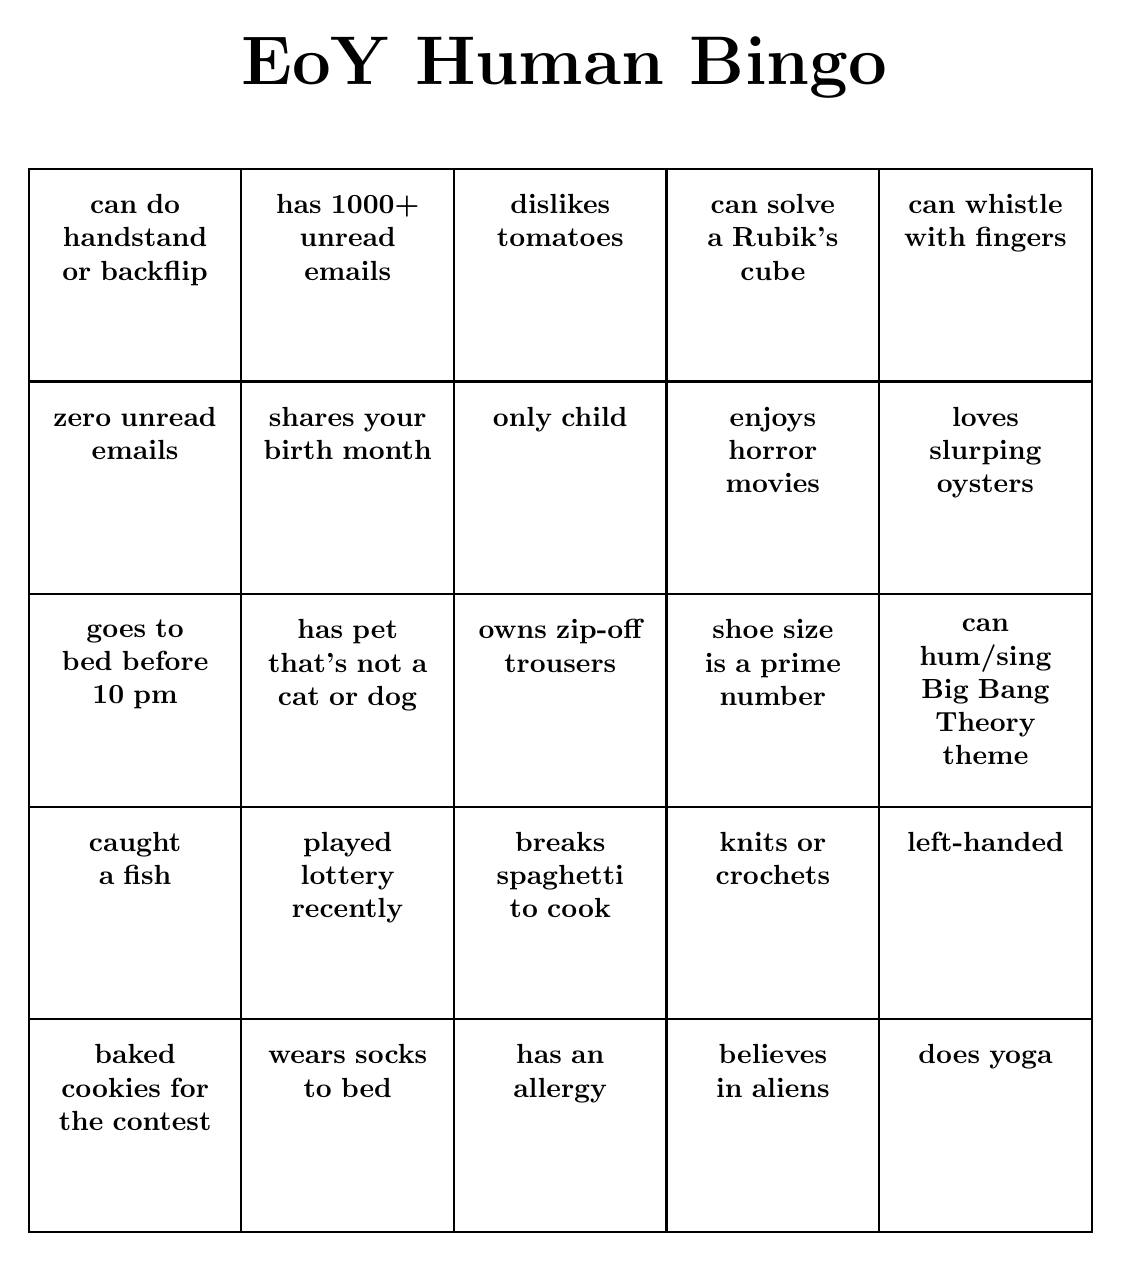
\begin{tikzpicture}
% Set the grid dimensions
\def\cellsize{2.7cm} % Each cell will be 2x2 cm

% Draw the grid and insert the numbers
\draw[thick] (0.0, 0.0) rectangle +(2.7, 2.7);
\node[anchor=north, align=center, text width=2.2cm] at (1.35, 2.5) {\textbf{can do handstand or backflip}};
\draw[thick] (2.7, 0.0) rectangle +(2.7, 2.7);
\node[anchor=north, align=center, text width=2.2cm] at (4.050000000000001, 2.5) {\textbf{has 1000+ unread emails}};
\draw[thick] (5.4, 0.0) rectangle +(2.7, 2.7);
\node[anchor=north, align=center, text width=2.2cm] at (6.75, 2.5) {\textbf{dislikes tomatoes}};
\draw[thick] (8.100000000000001, 0.0) rectangle +(2.7, 2.7);
\node[anchor=north, align=center, text width=2.2cm] at (9.450000000000001, 2.5) {\textbf{can solve a Rubik's cube}};
\draw[thick] (10.8, 0.0) rectangle +(2.7, 2.7);
\node[anchor=north, align=center, text width=2.2cm] at (12.15, 2.5) {\textbf{can whistle with fingers}};
\draw[thick] (0.0, -2.7) rectangle +(2.7, 2.7);
\node[anchor=north, align=center, text width=2.2cm] at (1.35, -0.2) {\textbf{zero unread emails}};
\draw[thick] (2.7, -2.7) rectangle +(2.7, 2.7);
\node[anchor=north, align=center, text width=2.2cm] at (4.050000000000001, -0.2) {\textbf{shares your birth month}};
\draw[thick] (5.4, -2.7) rectangle +(2.7, 2.7);
\node[anchor=north, align=center, text width=2.2cm] at (6.75, -0.2) {\textbf{only child}};
\draw[thick] (8.100000000000001, -2.7) rectangle +(2.7, 2.7);
\node[anchor=north, align=center, text width=2.2cm] at (9.450000000000001, -0.2) {\textbf{enjoys horror movies}};
\draw[thick] (10.8, -2.7) rectangle +(2.7, 2.7);
\node[anchor=north, align=center, text width=2.2cm] at (12.15, -0.2) {\textbf{loves slurping oysters}};
\draw[thick] (0.0, -5.4) rectangle +(2.7, 2.7);
\node[anchor=north, align=center, text width=2.2cm] at (1.35, -2.9000000000000004) {\textbf{goes to bed before 10 pm}};
\draw[thick] (2.7, -5.4) rectangle +(2.7, 2.7);
\node[anchor=north, align=center, text width=2.2cm] at (4.050000000000001, -2.9000000000000004) {\textbf{has pet that's not a cat or dog}};
\draw[thick] (5.4, -5.4) rectangle +(2.7, 2.7);
\node[anchor=north, align=center, text width=2.2cm] at (6.75, -2.9000000000000004) {\textbf{owns zip-off trousers}};
\draw[thick] (8.100000000000001, -5.4) rectangle +(2.7, 2.7);
\node[anchor=north, align=center, text width=2.2cm] at (9.450000000000001, -2.9000000000000004) {\textbf{shoe size is a prime number}};
\draw[thick] (10.8, -5.4) rectangle +(2.7, 2.7);
\node[anchor=north, align=center, text width=2.2cm] at (12.15, -2.9000000000000004) {\textbf{can hum/sing Big Bang Theory theme}};
\draw[thick] (0.0, -8.100000000000001) rectangle +(2.7, 2.7);
\node[anchor=north, align=center, text width=2.2cm] at (1.35, -5.600000000000001) {\textbf{caught a fish}};
\draw[thick] (2.7, -8.100000000000001) rectangle +(2.7, 2.7);
\node[anchor=north, align=center, text width=2.2cm] at (4.050000000000001, -5.600000000000001) {\textbf{played lottery recently}};
\draw[thick] (5.4, -8.100000000000001) rectangle +(2.7, 2.7);
\node[anchor=north, align=center, text width=2.2cm] at (6.75, -5.600000000000001) {\textbf{breaks spaghetti to cook}};
\draw[thick] (8.100000000000001, -8.100000000000001) rectangle +(2.7, 2.7);
\node[anchor=north, align=center, text width=2.2cm] at (9.450000000000001, -5.600000000000001) {\textbf{knits or crochets}};
\draw[thick] (10.8, -8.100000000000001) rectangle +(2.7, 2.7);
\node[anchor=north, align=center, text width=2.2cm] at (12.15, -5.600000000000001) {\textbf{left-handed}};
\draw[thick] (0.0, -10.8) rectangle +(2.7, 2.7);
\node[anchor=north, align=center, text width=2.2cm] at (1.35, -8.3) {\textbf{baked cookies for the contest}};
\draw[thick] (2.7, -10.8) rectangle +(2.7, 2.7);
\node[anchor=north, align=center, text width=2.2cm] at (4.050000000000001, -8.3) {\textbf{wears socks to bed}};
\draw[thick] (5.4, -10.8) rectangle +(2.7, 2.7);
\node[anchor=north, align=center, text width=2.2cm] at (6.75, -8.3) {\textbf{has an allergy}};
\draw[thick] (8.100000000000001, -10.8) rectangle +(2.7, 2.7);
\node[anchor=north, align=center, text width=2.2cm] at (9.450000000000001, -8.3) {\textbf{believes in aliens}};
\draw[thick] (10.8, -10.8) rectangle +(2.7, 2.7);
\node[anchor=north, align=center, text width=2.2cm] at (12.15, -8.3) {\textbf{does yoga}};
\node[anchor=north, font = \Huge] at (6.8, 4.5){\textbf{EoY Human Bingo}};
\end{tikzpicture}
\end{center}
\newpage\begin{center}
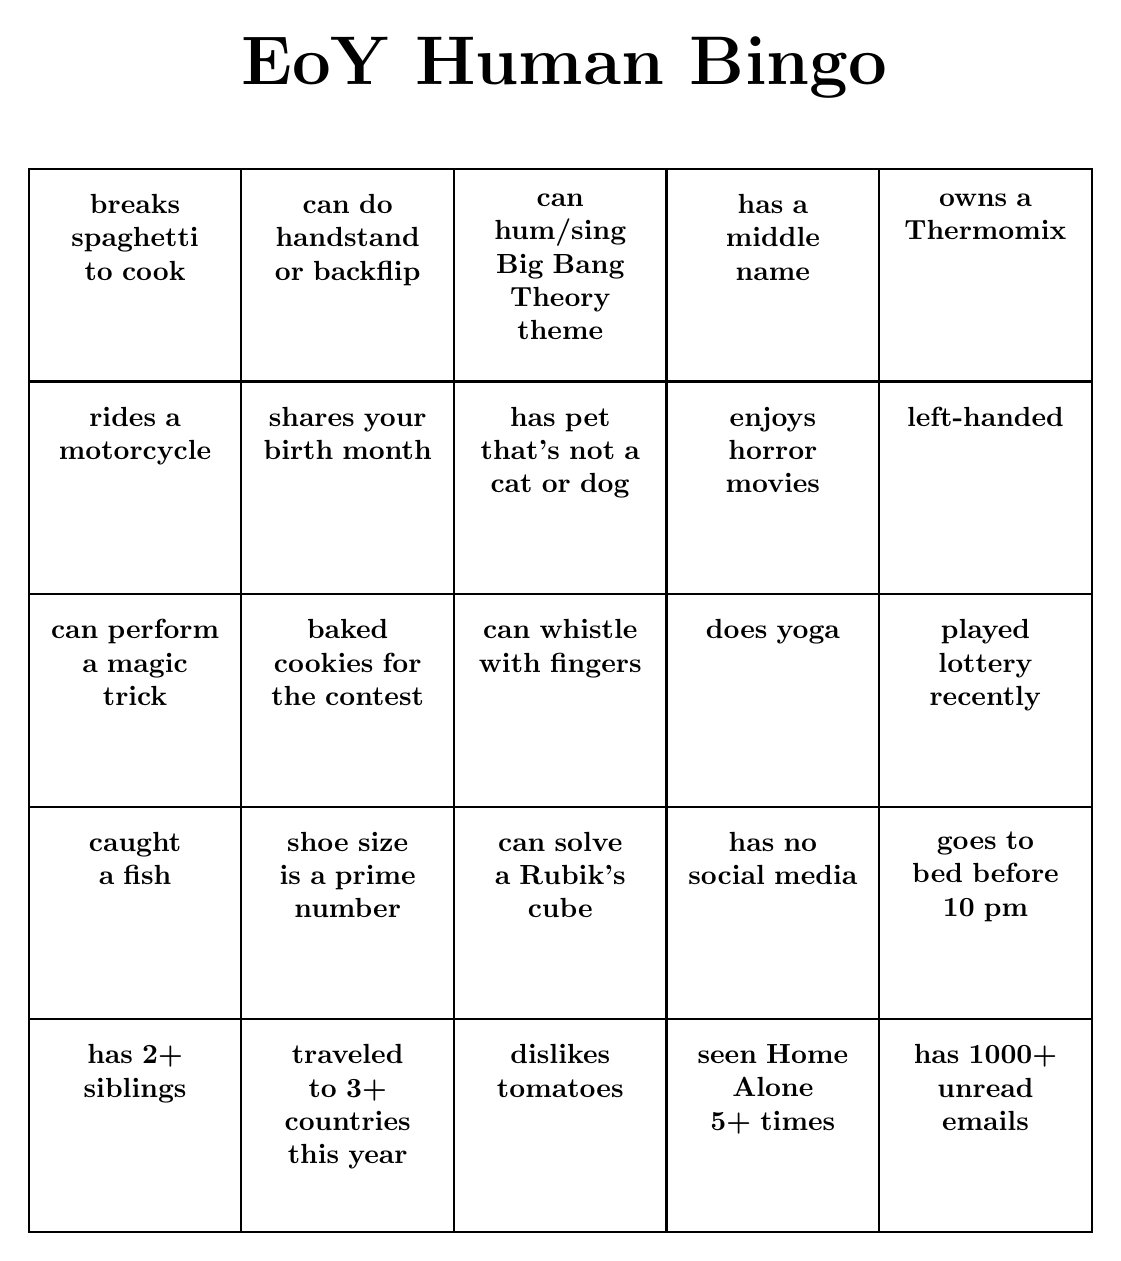
\begin{tikzpicture}
% Set the grid dimensions
\def\cellsize{2.7cm} % Each cell will be 2x2 cm

% Draw the grid and insert the numbers
\draw[thick] (0.0, 0.0) rectangle +(2.7, 2.7);
\node[anchor=north, align=center, text width=2.2cm] at (1.35, 2.5) {\textbf{breaks spaghetti to cook}};
\draw[thick] (2.7, 0.0) rectangle +(2.7, 2.7);
\node[anchor=north, align=center, text width=2.2cm] at (4.050000000000001, 2.5) {\textbf{can do handstand or backflip}};
\draw[thick] (5.4, 0.0) rectangle +(2.7, 2.7);
\node[anchor=north, align=center, text width=2.2cm] at (6.75, 2.5) {\textbf{can hum/sing Big Bang Theory theme}};
\draw[thick] (8.100000000000001, 0.0) rectangle +(2.7, 2.7);
\node[anchor=north, align=center, text width=2.2cm] at (9.450000000000001, 2.5) {\textbf{has a middle name}};
\draw[thick] (10.8, 0.0) rectangle +(2.7, 2.7);
\node[anchor=north, align=center, text width=2.2cm] at (12.15, 2.5) {\textbf{owns a Thermomix}};
\draw[thick] (0.0, -2.7) rectangle +(2.7, 2.7);
\node[anchor=north, align=center, text width=2.2cm] at (1.35, -0.2) {\textbf{rides a motorcycle}};
\draw[thick] (2.7, -2.7) rectangle +(2.7, 2.7);
\node[anchor=north, align=center, text width=2.2cm] at (4.050000000000001, -0.2) {\textbf{shares your birth month}};
\draw[thick] (5.4, -2.7) rectangle +(2.7, 2.7);
\node[anchor=north, align=center, text width=2.2cm] at (6.75, -0.2) {\textbf{has pet that's not a cat or dog}};
\draw[thick] (8.100000000000001, -2.7) rectangle +(2.7, 2.7);
\node[anchor=north, align=center, text width=2.2cm] at (9.450000000000001, -0.2) {\textbf{enjoys horror movies}};
\draw[thick] (10.8, -2.7) rectangle +(2.7, 2.7);
\node[anchor=north, align=center, text width=2.2cm] at (12.15, -0.2) {\textbf{left-handed}};
\draw[thick] (0.0, -5.4) rectangle +(2.7, 2.7);
\node[anchor=north, align=center, text width=2.2cm] at (1.35, -2.9000000000000004) {\textbf{can perform a magic trick}};
\draw[thick] (2.7, -5.4) rectangle +(2.7, 2.7);
\node[anchor=north, align=center, text width=2.2cm] at (4.050000000000001, -2.9000000000000004) {\textbf{baked cookies for the contest}};
\draw[thick] (5.4, -5.4) rectangle +(2.7, 2.7);
\node[anchor=north, align=center, text width=2.2cm] at (6.75, -2.9000000000000004) {\textbf{can whistle with fingers}};
\draw[thick] (8.100000000000001, -5.4) rectangle +(2.7, 2.7);
\node[anchor=north, align=center, text width=2.2cm] at (9.450000000000001, -2.9000000000000004) {\textbf{does yoga}};
\draw[thick] (10.8, -5.4) rectangle +(2.7, 2.7);
\node[anchor=north, align=center, text width=2.2cm] at (12.15, -2.9000000000000004) {\textbf{played lottery recently}};
\draw[thick] (0.0, -8.100000000000001) rectangle +(2.7, 2.7);
\node[anchor=north, align=center, text width=2.2cm] at (1.35, -5.600000000000001) {\textbf{caught a fish}};
\draw[thick] (2.7, -8.100000000000001) rectangle +(2.7, 2.7);
\node[anchor=north, align=center, text width=2.2cm] at (4.050000000000001, -5.600000000000001) {\textbf{shoe size is a prime number}};
\draw[thick] (5.4, -8.100000000000001) rectangle +(2.7, 2.7);
\node[anchor=north, align=center, text width=2.2cm] at (6.75, -5.600000000000001) {\textbf{can solve a Rubik's cube}};
\draw[thick] (8.100000000000001, -8.100000000000001) rectangle +(2.7, 2.7);
\node[anchor=north, align=center, text width=2.2cm] at (9.450000000000001, -5.600000000000001) {\textbf{has no social media}};
\draw[thick] (10.8, -8.100000000000001) rectangle +(2.7, 2.7);
\node[anchor=north, align=center, text width=2.2cm] at (12.15, -5.600000000000001) {\textbf{goes to bed before 10 pm}};
\draw[thick] (0.0, -10.8) rectangle +(2.7, 2.7);
\node[anchor=north, align=center, text width=2.2cm] at (1.35, -8.3) {\textbf{has 2+ siblings}};
\draw[thick] (2.7, -10.8) rectangle +(2.7, 2.7);
\node[anchor=north, align=center, text width=2.2cm] at (4.050000000000001, -8.3) {\textbf{traveled to 3+ countries this year}};
\draw[thick] (5.4, -10.8) rectangle +(2.7, 2.7);
\node[anchor=north, align=center, text width=2.2cm] at (6.75, -8.3) {\textbf{dislikes tomatoes}};
\draw[thick] (8.100000000000001, -10.8) rectangle +(2.7, 2.7);
\node[anchor=north, align=center, text width=2.2cm] at (9.450000000000001, -8.3) {\textbf{seen Home Alone 5+ times}};
\draw[thick] (10.8, -10.8) rectangle +(2.7, 2.7);
\node[anchor=north, align=center, text width=2.2cm] at (12.15, -8.3) {\textbf{has 1000+ unread emails}};
\node[anchor=north, font = \Huge] at (6.8, 4.5){\textbf{EoY Human Bingo}};
\end{tikzpicture}
\end{center}
\newpage\begin{center}
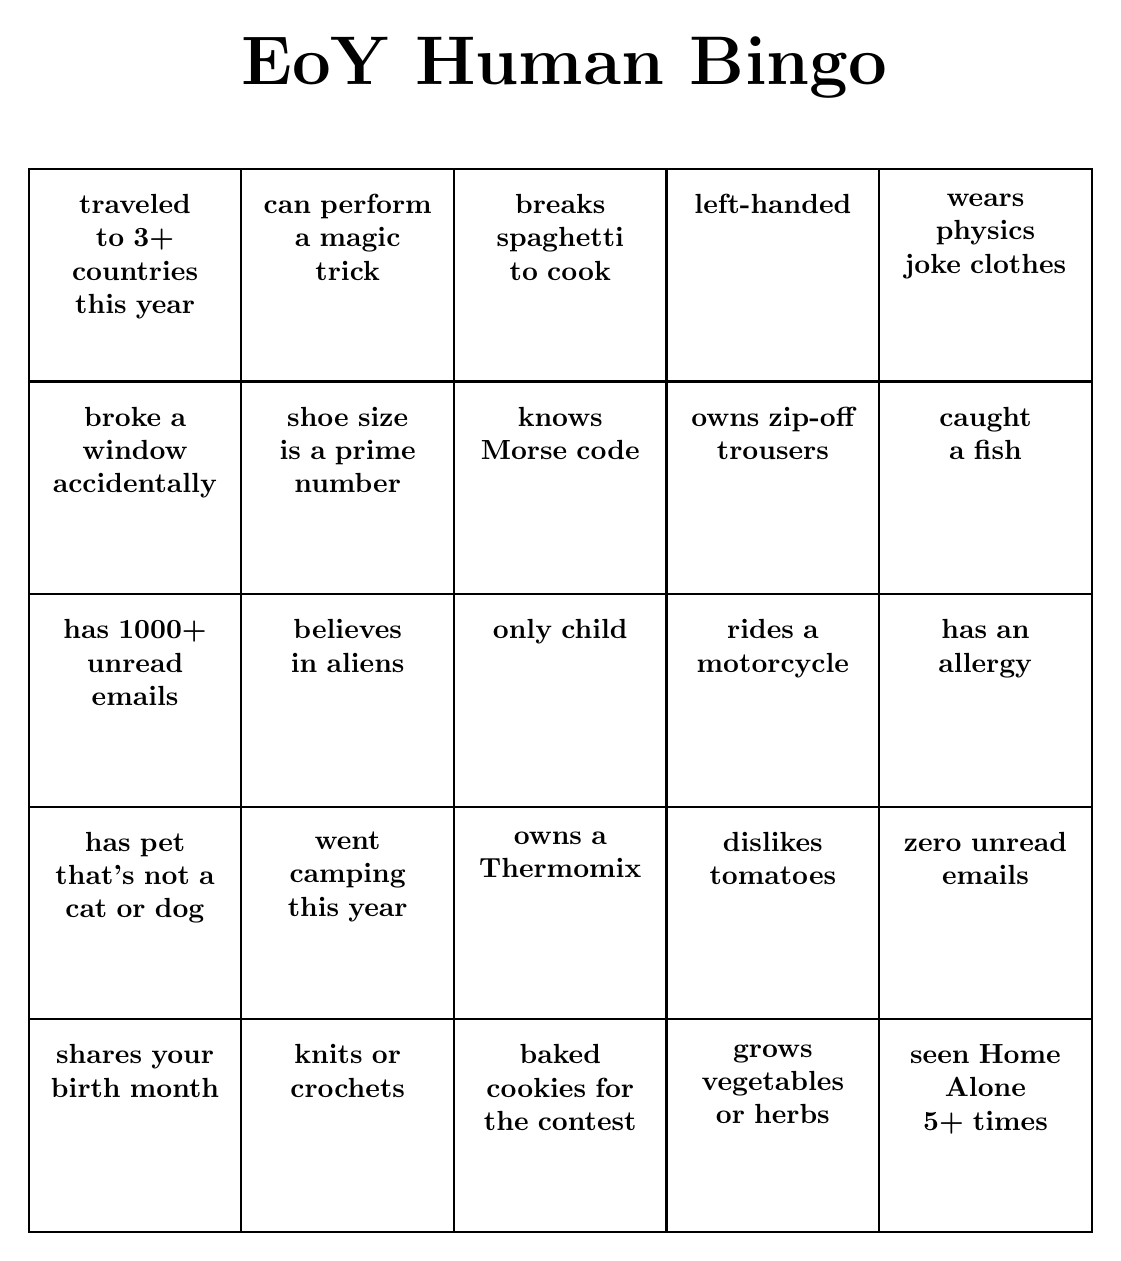
\begin{tikzpicture}
% Set the grid dimensions
\def\cellsize{2.7cm} % Each cell will be 2x2 cm

% Draw the grid and insert the numbers
\draw[thick] (0.0, 0.0) rectangle +(2.7, 2.7);
\node[anchor=north, align=center, text width=2.2cm] at (1.35, 2.5) {\textbf{traveled to 3+ countries this year}};
\draw[thick] (2.7, 0.0) rectangle +(2.7, 2.7);
\node[anchor=north, align=center, text width=2.2cm] at (4.050000000000001, 2.5) {\textbf{can perform a magic trick}};
\draw[thick] (5.4, 0.0) rectangle +(2.7, 2.7);
\node[anchor=north, align=center, text width=2.2cm] at (6.75, 2.5) {\textbf{breaks spaghetti to cook}};
\draw[thick] (8.100000000000001, 0.0) rectangle +(2.7, 2.7);
\node[anchor=north, align=center, text width=2.2cm] at (9.450000000000001, 2.5) {\textbf{left-handed}};
\draw[thick] (10.8, 0.0) rectangle +(2.7, 2.7);
\node[anchor=north, align=center, text width=2.2cm] at (12.15, 2.5) {\textbf{wears physics joke clothes}};
\draw[thick] (0.0, -2.7) rectangle +(2.7, 2.7);
\node[anchor=north, align=center, text width=2.2cm] at (1.35, -0.2) {\textbf{broke a window accidentally}};
\draw[thick] (2.7, -2.7) rectangle +(2.7, 2.7);
\node[anchor=north, align=center, text width=2.2cm] at (4.050000000000001, -0.2) {\textbf{shoe size is a prime number}};
\draw[thick] (5.4, -2.7) rectangle +(2.7, 2.7);
\node[anchor=north, align=center, text width=2.2cm] at (6.75, -0.2) {\textbf{knows Morse code}};
\draw[thick] (8.100000000000001, -2.7) rectangle +(2.7, 2.7);
\node[anchor=north, align=center, text width=2.2cm] at (9.450000000000001, -0.2) {\textbf{owns zip-off trousers}};
\draw[thick] (10.8, -2.7) rectangle +(2.7, 2.7);
\node[anchor=north, align=center, text width=2.2cm] at (12.15, -0.2) {\textbf{caught a fish}};
\draw[thick] (0.0, -5.4) rectangle +(2.7, 2.7);
\node[anchor=north, align=center, text width=2.2cm] at (1.35, -2.9000000000000004) {\textbf{has 1000+ unread emails}};
\draw[thick] (2.7, -5.4) rectangle +(2.7, 2.7);
\node[anchor=north, align=center, text width=2.2cm] at (4.050000000000001, -2.9000000000000004) {\textbf{believes in aliens}};
\draw[thick] (5.4, -5.4) rectangle +(2.7, 2.7);
\node[anchor=north, align=center, text width=2.2cm] at (6.75, -2.9000000000000004) {\textbf{only child}};
\draw[thick] (8.100000000000001, -5.4) rectangle +(2.7, 2.7);
\node[anchor=north, align=center, text width=2.2cm] at (9.450000000000001, -2.9000000000000004) {\textbf{rides a motorcycle}};
\draw[thick] (10.8, -5.4) rectangle +(2.7, 2.7);
\node[anchor=north, align=center, text width=2.2cm] at (12.15, -2.9000000000000004) {\textbf{has an allergy}};
\draw[thick] (0.0, -8.100000000000001) rectangle +(2.7, 2.7);
\node[anchor=north, align=center, text width=2.2cm] at (1.35, -5.600000000000001) {\textbf{has pet that's not a cat or dog}};
\draw[thick] (2.7, -8.100000000000001) rectangle +(2.7, 2.7);
\node[anchor=north, align=center, text width=2.2cm] at (4.050000000000001, -5.600000000000001) {\textbf{went camping this year}};
\draw[thick] (5.4, -8.100000000000001) rectangle +(2.7, 2.7);
\node[anchor=north, align=center, text width=2.2cm] at (6.75, -5.600000000000001) {\textbf{owns a Thermomix}};
\draw[thick] (8.100000000000001, -8.100000000000001) rectangle +(2.7, 2.7);
\node[anchor=north, align=center, text width=2.2cm] at (9.450000000000001, -5.600000000000001) {\textbf{dislikes tomatoes}};
\draw[thick] (10.8, -8.100000000000001) rectangle +(2.7, 2.7);
\node[anchor=north, align=center, text width=2.2cm] at (12.15, -5.600000000000001) {\textbf{zero unread emails}};
\draw[thick] (0.0, -10.8) rectangle +(2.7, 2.7);
\node[anchor=north, align=center, text width=2.2cm] at (1.35, -8.3) {\textbf{shares your birth month}};
\draw[thick] (2.7, -10.8) rectangle +(2.7, 2.7);
\node[anchor=north, align=center, text width=2.2cm] at (4.050000000000001, -8.3) {\textbf{knits or crochets}};
\draw[thick] (5.4, -10.8) rectangle +(2.7, 2.7);
\node[anchor=north, align=center, text width=2.2cm] at (6.75, -8.3) {\textbf{baked cookies for the contest}};
\draw[thick] (8.100000000000001, -10.8) rectangle +(2.7, 2.7);
\node[anchor=north, align=center, text width=2.2cm] at (9.450000000000001, -8.3) {\textbf{grows vegetables or herbs}};
\draw[thick] (10.8, -10.8) rectangle +(2.7, 2.7);
\node[anchor=north, align=center, text width=2.2cm] at (12.15, -8.3) {\textbf{seen Home Alone 5+ times}};
\node[anchor=north, font = \Huge] at (6.8, 4.5){\textbf{EoY Human Bingo}};
\end{tikzpicture}
\end{center}
\newpage\begin{center}
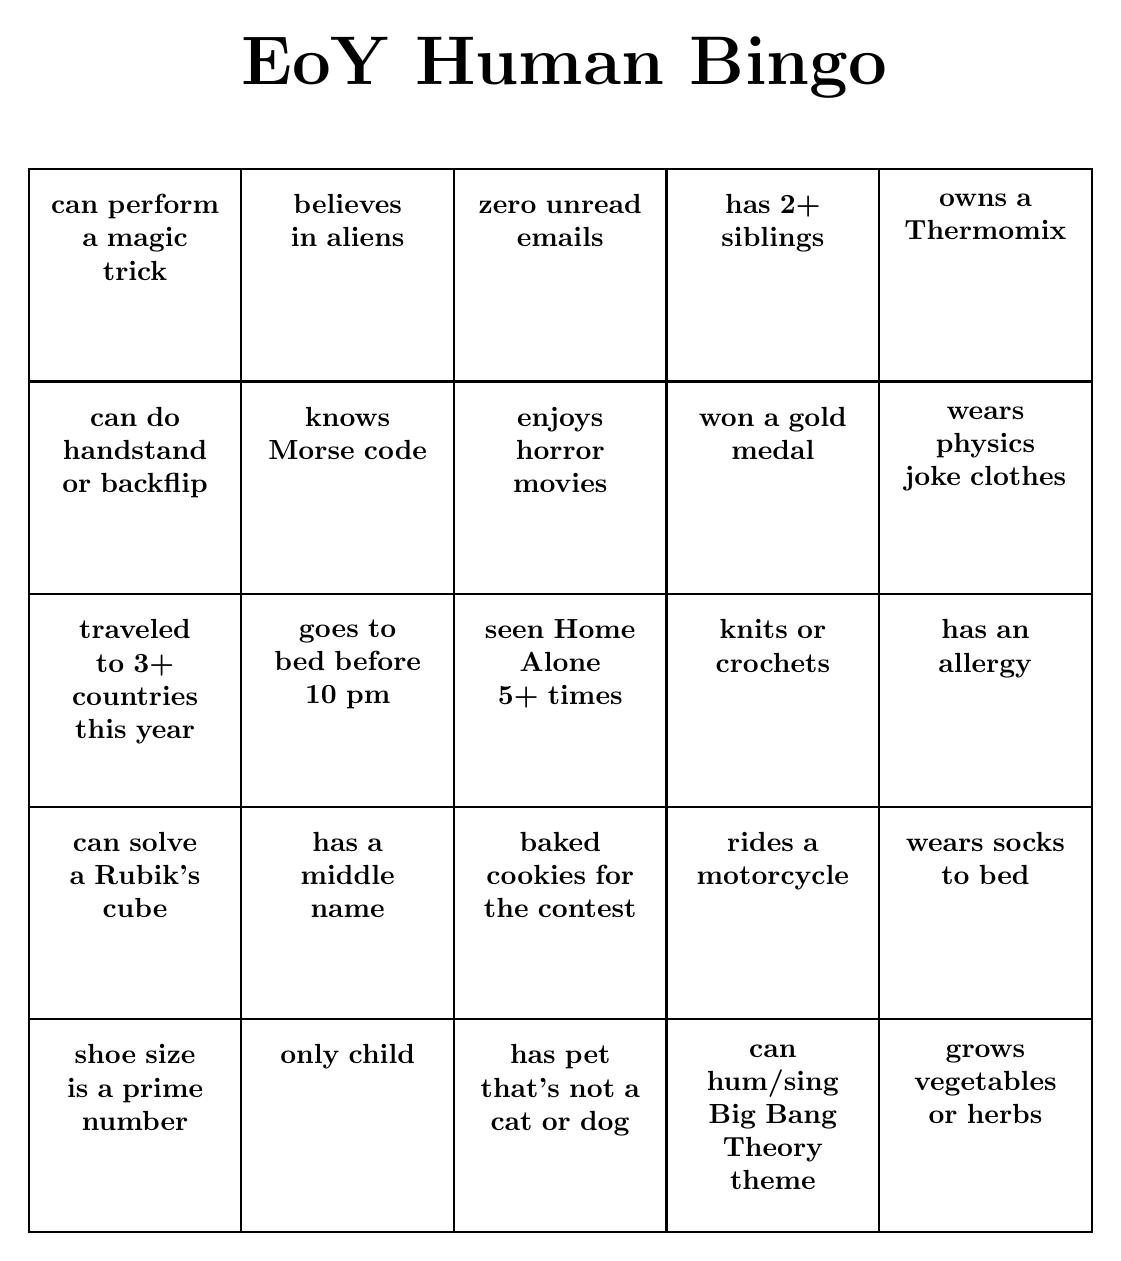
\begin{tikzpicture}
% Set the grid dimensions
\def\cellsize{2.7cm} % Each cell will be 2x2 cm

% Draw the grid and insert the numbers
\draw[thick] (0.0, 0.0) rectangle +(2.7, 2.7);
\node[anchor=north, align=center, text width=2.2cm] at (1.35, 2.5) {\textbf{can perform a magic trick}};
\draw[thick] (2.7, 0.0) rectangle +(2.7, 2.7);
\node[anchor=north, align=center, text width=2.2cm] at (4.050000000000001, 2.5) {\textbf{believes in aliens}};
\draw[thick] (5.4, 0.0) rectangle +(2.7, 2.7);
\node[anchor=north, align=center, text width=2.2cm] at (6.75, 2.5) {\textbf{zero unread emails}};
\draw[thick] (8.100000000000001, 0.0) rectangle +(2.7, 2.7);
\node[anchor=north, align=center, text width=2.2cm] at (9.450000000000001, 2.5) {\textbf{has 2+ siblings}};
\draw[thick] (10.8, 0.0) rectangle +(2.7, 2.7);
\node[anchor=north, align=center, text width=2.2cm] at (12.15, 2.5) {\textbf{owns a Thermomix}};
\draw[thick] (0.0, -2.7) rectangle +(2.7, 2.7);
\node[anchor=north, align=center, text width=2.2cm] at (1.35, -0.2) {\textbf{can do handstand or backflip}};
\draw[thick] (2.7, -2.7) rectangle +(2.7, 2.7);
\node[anchor=north, align=center, text width=2.2cm] at (4.050000000000001, -0.2) {\textbf{knows Morse code}};
\draw[thick] (5.4, -2.7) rectangle +(2.7, 2.7);
\node[anchor=north, align=center, text width=2.2cm] at (6.75, -0.2) {\textbf{enjoys horror movies}};
\draw[thick] (8.100000000000001, -2.7) rectangle +(2.7, 2.7);
\node[anchor=north, align=center, text width=2.2cm] at (9.450000000000001, -0.2) {\textbf{won a gold medal}};
\draw[thick] (10.8, -2.7) rectangle +(2.7, 2.7);
\node[anchor=north, align=center, text width=2.2cm] at (12.15, -0.2) {\textbf{wears physics joke clothes}};
\draw[thick] (0.0, -5.4) rectangle +(2.7, 2.7);
\node[anchor=north, align=center, text width=2.2cm] at (1.35, -2.9000000000000004) {\textbf{traveled to 3+ countries this year}};
\draw[thick] (2.7, -5.4) rectangle +(2.7, 2.7);
\node[anchor=north, align=center, text width=2.2cm] at (4.050000000000001, -2.9000000000000004) {\textbf{goes to bed before 10 pm}};
\draw[thick] (5.4, -5.4) rectangle +(2.7, 2.7);
\node[anchor=north, align=center, text width=2.2cm] at (6.75, -2.9000000000000004) {\textbf{seen Home Alone 5+ times}};
\draw[thick] (8.100000000000001, -5.4) rectangle +(2.7, 2.7);
\node[anchor=north, align=center, text width=2.2cm] at (9.450000000000001, -2.9000000000000004) {\textbf{knits or crochets}};
\draw[thick] (10.8, -5.4) rectangle +(2.7, 2.7);
\node[anchor=north, align=center, text width=2.2cm] at (12.15, -2.9000000000000004) {\textbf{has an allergy}};
\draw[thick] (0.0, -8.100000000000001) rectangle +(2.7, 2.7);
\node[anchor=north, align=center, text width=2.2cm] at (1.35, -5.600000000000001) {\textbf{can solve a Rubik's cube}};
\draw[thick] (2.7, -8.100000000000001) rectangle +(2.7, 2.7);
\node[anchor=north, align=center, text width=2.2cm] at (4.050000000000001, -5.600000000000001) {\textbf{has a middle name}};
\draw[thick] (5.4, -8.100000000000001) rectangle +(2.7, 2.7);
\node[anchor=north, align=center, text width=2.2cm] at (6.75, -5.600000000000001) {\textbf{baked cookies for the contest}};
\draw[thick] (8.100000000000001, -8.100000000000001) rectangle +(2.7, 2.7);
\node[anchor=north, align=center, text width=2.2cm] at (9.450000000000001, -5.600000000000001) {\textbf{rides a motorcycle}};
\draw[thick] (10.8, -8.100000000000001) rectangle +(2.7, 2.7);
\node[anchor=north, align=center, text width=2.2cm] at (12.15, -5.600000000000001) {\textbf{wears socks to bed}};
\draw[thick] (0.0, -10.8) rectangle +(2.7, 2.7);
\node[anchor=north, align=center, text width=2.2cm] at (1.35, -8.3) {\textbf{shoe size is a prime number}};
\draw[thick] (2.7, -10.8) rectangle +(2.7, 2.7);
\node[anchor=north, align=center, text width=2.2cm] at (4.050000000000001, -8.3) {\textbf{only child}};
\draw[thick] (5.4, -10.8) rectangle +(2.7, 2.7);
\node[anchor=north, align=center, text width=2.2cm] at (6.75, -8.3) {\textbf{has pet that's not a cat or dog}};
\draw[thick] (8.100000000000001, -10.8) rectangle +(2.7, 2.7);
\node[anchor=north, align=center, text width=2.2cm] at (9.450000000000001, -8.3) {\textbf{can hum/sing Big Bang Theory theme}};
\draw[thick] (10.8, -10.8) rectangle +(2.7, 2.7);
\node[anchor=north, align=center, text width=2.2cm] at (12.15, -8.3) {\textbf{grows vegetables or herbs}};
\node[anchor=north, font = \Huge] at (6.8, 4.5){\textbf{EoY Human Bingo}};
\end{tikzpicture}
\end{center}
\newpage\begin{center}
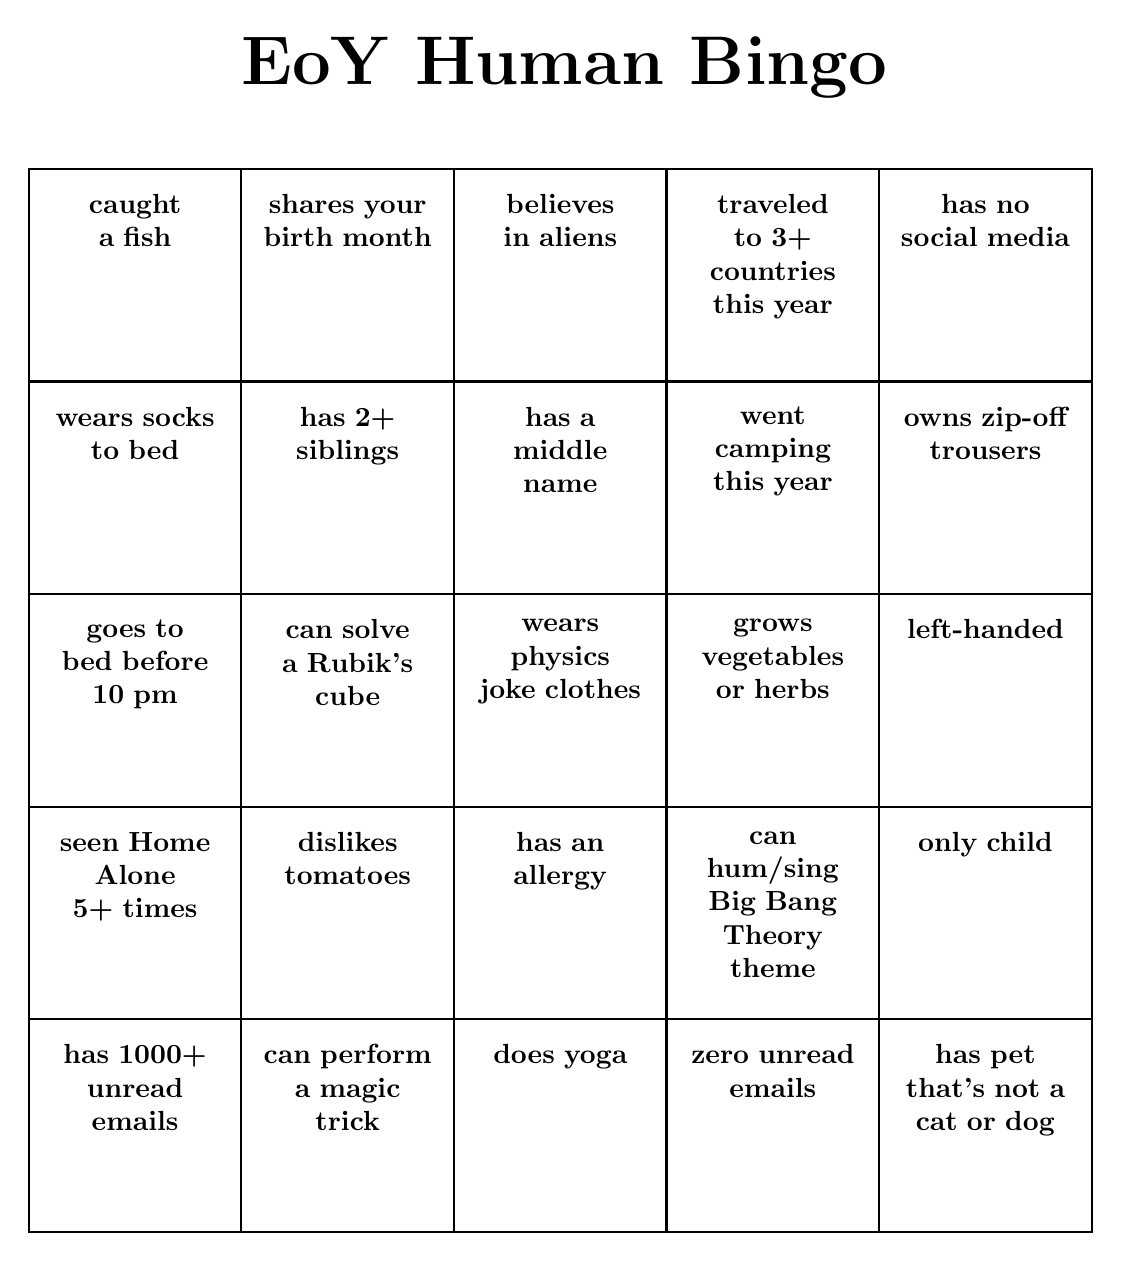
\begin{tikzpicture}
% Set the grid dimensions
\def\cellsize{2.7cm} % Each cell will be 2x2 cm

% Draw the grid and insert the numbers
\draw[thick] (0.0, 0.0) rectangle +(2.7, 2.7);
\node[anchor=north, align=center, text width=2.2cm] at (1.35, 2.5) {\textbf{caught a fish}};
\draw[thick] (2.7, 0.0) rectangle +(2.7, 2.7);
\node[anchor=north, align=center, text width=2.2cm] at (4.050000000000001, 2.5) {\textbf{shares your birth month}};
\draw[thick] (5.4, 0.0) rectangle +(2.7, 2.7);
\node[anchor=north, align=center, text width=2.2cm] at (6.75, 2.5) {\textbf{believes in aliens}};
\draw[thick] (8.100000000000001, 0.0) rectangle +(2.7, 2.7);
\node[anchor=north, align=center, text width=2.2cm] at (9.450000000000001, 2.5) {\textbf{traveled to 3+ countries this year}};
\draw[thick] (10.8, 0.0) rectangle +(2.7, 2.7);
\node[anchor=north, align=center, text width=2.2cm] at (12.15, 2.5) {\textbf{has no social media}};
\draw[thick] (0.0, -2.7) rectangle +(2.7, 2.7);
\node[anchor=north, align=center, text width=2.2cm] at (1.35, -0.2) {\textbf{wears socks to bed}};
\draw[thick] (2.7, -2.7) rectangle +(2.7, 2.7);
\node[anchor=north, align=center, text width=2.2cm] at (4.050000000000001, -0.2) {\textbf{has 2+ siblings}};
\draw[thick] (5.4, -2.7) rectangle +(2.7, 2.7);
\node[anchor=north, align=center, text width=2.2cm] at (6.75, -0.2) {\textbf{has a middle name}};
\draw[thick] (8.100000000000001, -2.7) rectangle +(2.7, 2.7);
\node[anchor=north, align=center, text width=2.2cm] at (9.450000000000001, -0.2) {\textbf{went camping this year}};
\draw[thick] (10.8, -2.7) rectangle +(2.7, 2.7);
\node[anchor=north, align=center, text width=2.2cm] at (12.15, -0.2) {\textbf{owns zip-off trousers}};
\draw[thick] (0.0, -5.4) rectangle +(2.7, 2.7);
\node[anchor=north, align=center, text width=2.2cm] at (1.35, -2.9000000000000004) {\textbf{goes to bed before 10 pm}};
\draw[thick] (2.7, -5.4) rectangle +(2.7, 2.7);
\node[anchor=north, align=center, text width=2.2cm] at (4.050000000000001, -2.9000000000000004) {\textbf{can solve a Rubik's cube}};
\draw[thick] (5.4, -5.4) rectangle +(2.7, 2.7);
\node[anchor=north, align=center, text width=2.2cm] at (6.75, -2.9000000000000004) {\textbf{wears physics joke clothes}};
\draw[thick] (8.100000000000001, -5.4) rectangle +(2.7, 2.7);
\node[anchor=north, align=center, text width=2.2cm] at (9.450000000000001, -2.9000000000000004) {\textbf{grows vegetables or herbs}};
\draw[thick] (10.8, -5.4) rectangle +(2.7, 2.7);
\node[anchor=north, align=center, text width=2.2cm] at (12.15, -2.9000000000000004) {\textbf{left-handed}};
\draw[thick] (0.0, -8.100000000000001) rectangle +(2.7, 2.7);
\node[anchor=north, align=center, text width=2.2cm] at (1.35, -5.600000000000001) {\textbf{seen Home Alone 5+ times}};
\draw[thick] (2.7, -8.100000000000001) rectangle +(2.7, 2.7);
\node[anchor=north, align=center, text width=2.2cm] at (4.050000000000001, -5.600000000000001) {\textbf{dislikes tomatoes}};
\draw[thick] (5.4, -8.100000000000001) rectangle +(2.7, 2.7);
\node[anchor=north, align=center, text width=2.2cm] at (6.75, -5.600000000000001) {\textbf{has an allergy}};
\draw[thick] (8.100000000000001, -8.100000000000001) rectangle +(2.7, 2.7);
\node[anchor=north, align=center, text width=2.2cm] at (9.450000000000001, -5.600000000000001) {\textbf{can hum/sing Big Bang Theory theme}};
\draw[thick] (10.8, -8.100000000000001) rectangle +(2.7, 2.7);
\node[anchor=north, align=center, text width=2.2cm] at (12.15, -5.600000000000001) {\textbf{only child}};
\draw[thick] (0.0, -10.8) rectangle +(2.7, 2.7);
\node[anchor=north, align=center, text width=2.2cm] at (1.35, -8.3) {\textbf{has 1000+ unread emails}};
\draw[thick] (2.7, -10.8) rectangle +(2.7, 2.7);
\node[anchor=north, align=center, text width=2.2cm] at (4.050000000000001, -8.3) {\textbf{can perform a magic trick}};
\draw[thick] (5.4, -10.8) rectangle +(2.7, 2.7);
\node[anchor=north, align=center, text width=2.2cm] at (6.75, -8.3) {\textbf{does yoga}};
\draw[thick] (8.100000000000001, -10.8) rectangle +(2.7, 2.7);
\node[anchor=north, align=center, text width=2.2cm] at (9.450000000000001, -8.3) {\textbf{zero unread emails}};
\draw[thick] (10.8, -10.8) rectangle +(2.7, 2.7);
\node[anchor=north, align=center, text width=2.2cm] at (12.15, -8.3) {\textbf{has pet that's not a cat or dog}};
\node[anchor=north, font = \Huge] at (6.8, 4.5){\textbf{EoY Human Bingo}};
\end{tikzpicture}
\end{center}
\newpage\begin{center}
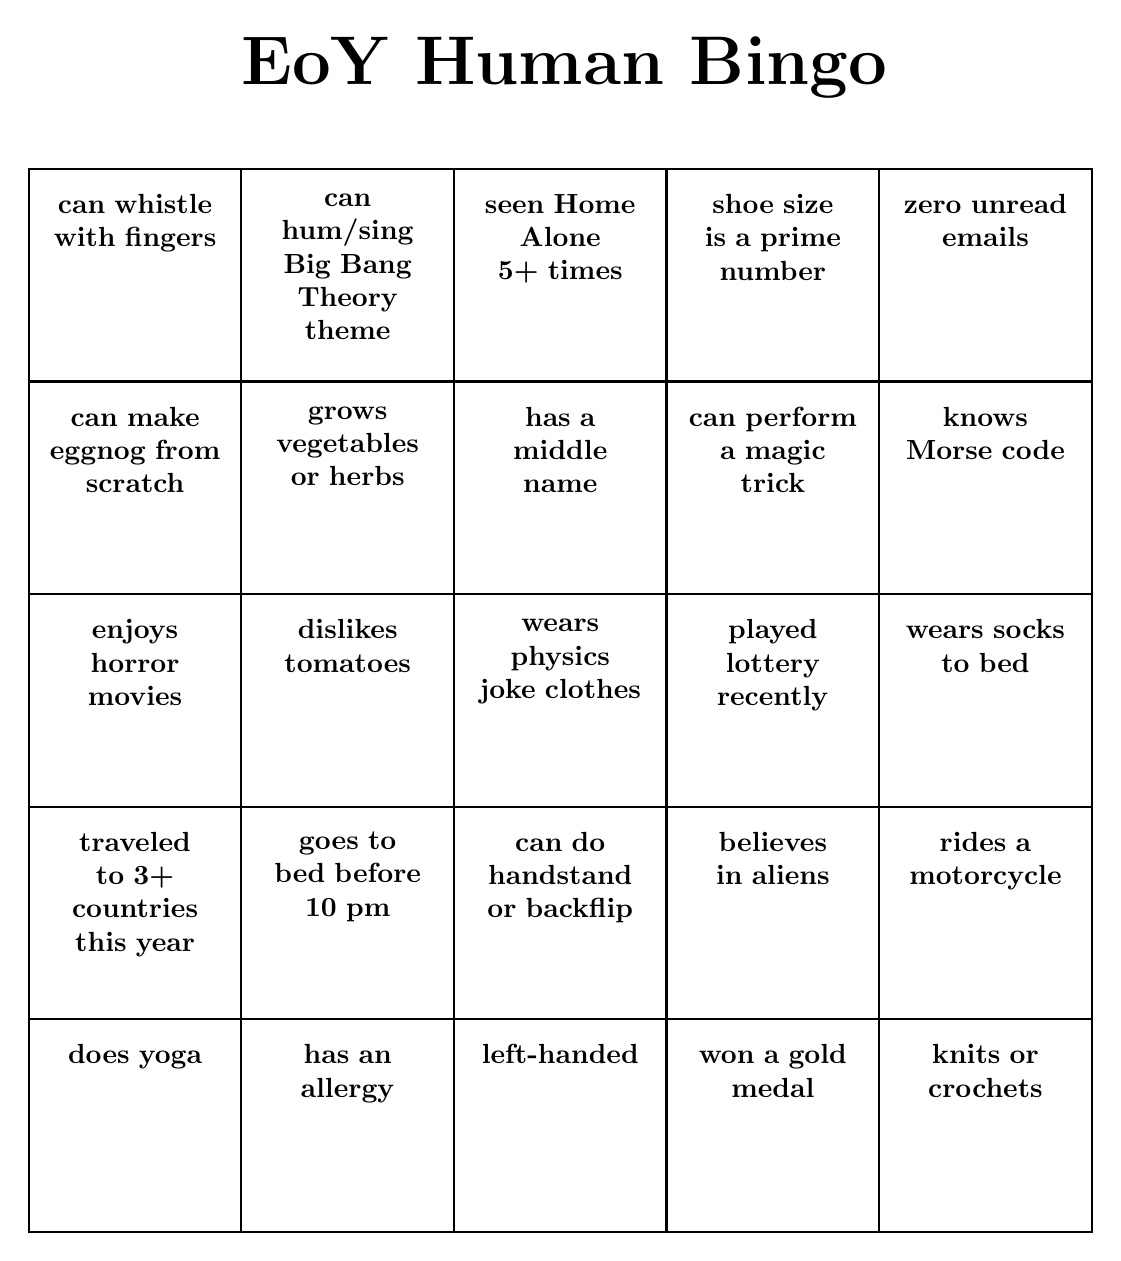
\begin{tikzpicture}
% Set the grid dimensions
\def\cellsize{2.7cm} % Each cell will be 2x2 cm

% Draw the grid and insert the numbers
\draw[thick] (0.0, 0.0) rectangle +(2.7, 2.7);
\node[anchor=north, align=center, text width=2.2cm] at (1.35, 2.5) {\textbf{can whistle with fingers}};
\draw[thick] (2.7, 0.0) rectangle +(2.7, 2.7);
\node[anchor=north, align=center, text width=2.2cm] at (4.050000000000001, 2.5) {\textbf{can hum/sing Big Bang Theory theme}};
\draw[thick] (5.4, 0.0) rectangle +(2.7, 2.7);
\node[anchor=north, align=center, text width=2.2cm] at (6.75, 2.5) {\textbf{seen Home Alone 5+ times}};
\draw[thick] (8.100000000000001, 0.0) rectangle +(2.7, 2.7);
\node[anchor=north, align=center, text width=2.2cm] at (9.450000000000001, 2.5) {\textbf{shoe size is a prime number}};
\draw[thick] (10.8, 0.0) rectangle +(2.7, 2.7);
\node[anchor=north, align=center, text width=2.2cm] at (12.15, 2.5) {\textbf{zero unread emails}};
\draw[thick] (0.0, -2.7) rectangle +(2.7, 2.7);
\node[anchor=north, align=center, text width=2.2cm] at (1.35, -0.2) {\textbf{can make eggnog from scratch}};
\draw[thick] (2.7, -2.7) rectangle +(2.7, 2.7);
\node[anchor=north, align=center, text width=2.2cm] at (4.050000000000001, -0.2) {\textbf{grows vegetables or herbs}};
\draw[thick] (5.4, -2.7) rectangle +(2.7, 2.7);
\node[anchor=north, align=center, text width=2.2cm] at (6.75, -0.2) {\textbf{has a middle name}};
\draw[thick] (8.100000000000001, -2.7) rectangle +(2.7, 2.7);
\node[anchor=north, align=center, text width=2.2cm] at (9.450000000000001, -0.2) {\textbf{can perform a magic trick}};
\draw[thick] (10.8, -2.7) rectangle +(2.7, 2.7);
\node[anchor=north, align=center, text width=2.2cm] at (12.15, -0.2) {\textbf{knows Morse code}};
\draw[thick] (0.0, -5.4) rectangle +(2.7, 2.7);
\node[anchor=north, align=center, text width=2.2cm] at (1.35, -2.9000000000000004) {\textbf{enjoys horror movies}};
\draw[thick] (2.7, -5.4) rectangle +(2.7, 2.7);
\node[anchor=north, align=center, text width=2.2cm] at (4.050000000000001, -2.9000000000000004) {\textbf{dislikes tomatoes}};
\draw[thick] (5.4, -5.4) rectangle +(2.7, 2.7);
\node[anchor=north, align=center, text width=2.2cm] at (6.75, -2.9000000000000004) {\textbf{wears physics joke clothes}};
\draw[thick] (8.100000000000001, -5.4) rectangle +(2.7, 2.7);
\node[anchor=north, align=center, text width=2.2cm] at (9.450000000000001, -2.9000000000000004) {\textbf{played lottery recently}};
\draw[thick] (10.8, -5.4) rectangle +(2.7, 2.7);
\node[anchor=north, align=center, text width=2.2cm] at (12.15, -2.9000000000000004) {\textbf{wears socks to bed}};
\draw[thick] (0.0, -8.100000000000001) rectangle +(2.7, 2.7);
\node[anchor=north, align=center, text width=2.2cm] at (1.35, -5.600000000000001) {\textbf{traveled to 3+ countries this year}};
\draw[thick] (2.7, -8.100000000000001) rectangle +(2.7, 2.7);
\node[anchor=north, align=center, text width=2.2cm] at (4.050000000000001, -5.600000000000001) {\textbf{goes to bed before 10 pm}};
\draw[thick] (5.4, -8.100000000000001) rectangle +(2.7, 2.7);
\node[anchor=north, align=center, text width=2.2cm] at (6.75, -5.600000000000001) {\textbf{can do handstand or backflip}};
\draw[thick] (8.100000000000001, -8.100000000000001) rectangle +(2.7, 2.7);
\node[anchor=north, align=center, text width=2.2cm] at (9.450000000000001, -5.600000000000001) {\textbf{believes in aliens}};
\draw[thick] (10.8, -8.100000000000001) rectangle +(2.7, 2.7);
\node[anchor=north, align=center, text width=2.2cm] at (12.15, -5.600000000000001) {\textbf{rides a motorcycle}};
\draw[thick] (0.0, -10.8) rectangle +(2.7, 2.7);
\node[anchor=north, align=center, text width=2.2cm] at (1.35, -8.3) {\textbf{does yoga}};
\draw[thick] (2.7, -10.8) rectangle +(2.7, 2.7);
\node[anchor=north, align=center, text width=2.2cm] at (4.050000000000001, -8.3) {\textbf{has an allergy}};
\draw[thick] (5.4, -10.8) rectangle +(2.7, 2.7);
\node[anchor=north, align=center, text width=2.2cm] at (6.75, -8.3) {\textbf{left-handed}};
\draw[thick] (8.100000000000001, -10.8) rectangle +(2.7, 2.7);
\node[anchor=north, align=center, text width=2.2cm] at (9.450000000000001, -8.3) {\textbf{won a gold medal}};
\draw[thick] (10.8, -10.8) rectangle +(2.7, 2.7);
\node[anchor=north, align=center, text width=2.2cm] at (12.15, -8.3) {\textbf{knits or crochets}};
\node[anchor=north, font = \Huge] at (6.8, 4.5){\textbf{EoY Human Bingo}};
\end{tikzpicture}
\end{center}
\newpage\begin{center}
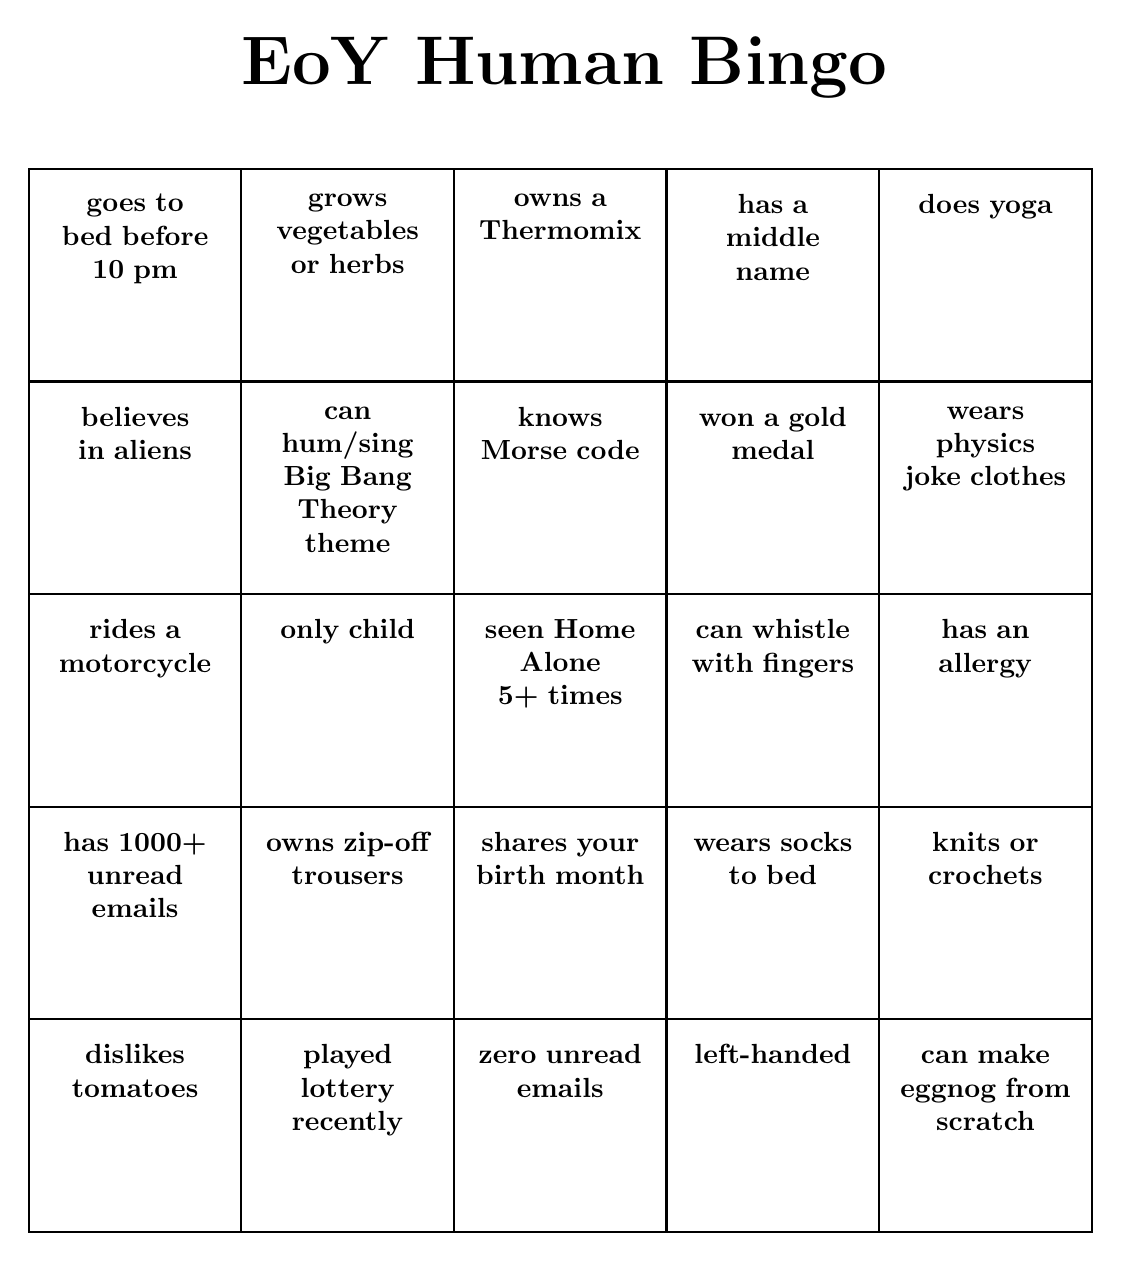
\begin{tikzpicture}
% Set the grid dimensions
\def\cellsize{2.7cm} % Each cell will be 2x2 cm

% Draw the grid and insert the numbers
\draw[thick] (0.0, 0.0) rectangle +(2.7, 2.7);
\node[anchor=north, align=center, text width=2.2cm] at (1.35, 2.5) {\textbf{goes to bed before 10 pm}};
\draw[thick] (2.7, 0.0) rectangle +(2.7, 2.7);
\node[anchor=north, align=center, text width=2.2cm] at (4.050000000000001, 2.5) {\textbf{grows vegetables or herbs}};
\draw[thick] (5.4, 0.0) rectangle +(2.7, 2.7);
\node[anchor=north, align=center, text width=2.2cm] at (6.75, 2.5) {\textbf{owns a Thermomix}};
\draw[thick] (8.100000000000001, 0.0) rectangle +(2.7, 2.7);
\node[anchor=north, align=center, text width=2.2cm] at (9.450000000000001, 2.5) {\textbf{has a middle name}};
\draw[thick] (10.8, 0.0) rectangle +(2.7, 2.7);
\node[anchor=north, align=center, text width=2.2cm] at (12.15, 2.5) {\textbf{does yoga}};
\draw[thick] (0.0, -2.7) rectangle +(2.7, 2.7);
\node[anchor=north, align=center, text width=2.2cm] at (1.35, -0.2) {\textbf{believes in aliens}};
\draw[thick] (2.7, -2.7) rectangle +(2.7, 2.7);
\node[anchor=north, align=center, text width=2.2cm] at (4.050000000000001, -0.2) {\textbf{can hum/sing Big Bang Theory theme}};
\draw[thick] (5.4, -2.7) rectangle +(2.7, 2.7);
\node[anchor=north, align=center, text width=2.2cm] at (6.75, -0.2) {\textbf{knows Morse code}};
\draw[thick] (8.100000000000001, -2.7) rectangle +(2.7, 2.7);
\node[anchor=north, align=center, text width=2.2cm] at (9.450000000000001, -0.2) {\textbf{won a gold medal}};
\draw[thick] (10.8, -2.7) rectangle +(2.7, 2.7);
\node[anchor=north, align=center, text width=2.2cm] at (12.15, -0.2) {\textbf{wears physics joke clothes}};
\draw[thick] (0.0, -5.4) rectangle +(2.7, 2.7);
\node[anchor=north, align=center, text width=2.2cm] at (1.35, -2.9000000000000004) {\textbf{rides a motorcycle}};
\draw[thick] (2.7, -5.4) rectangle +(2.7, 2.7);
\node[anchor=north, align=center, text width=2.2cm] at (4.050000000000001, -2.9000000000000004) {\textbf{only child}};
\draw[thick] (5.4, -5.4) rectangle +(2.7, 2.7);
\node[anchor=north, align=center, text width=2.2cm] at (6.75, -2.9000000000000004) {\textbf{seen Home Alone 5+ times}};
\draw[thick] (8.100000000000001, -5.4) rectangle +(2.7, 2.7);
\node[anchor=north, align=center, text width=2.2cm] at (9.450000000000001, -2.9000000000000004) {\textbf{can whistle with fingers}};
\draw[thick] (10.8, -5.4) rectangle +(2.7, 2.7);
\node[anchor=north, align=center, text width=2.2cm] at (12.15, -2.9000000000000004) {\textbf{has an allergy}};
\draw[thick] (0.0, -8.100000000000001) rectangle +(2.7, 2.7);
\node[anchor=north, align=center, text width=2.2cm] at (1.35, -5.600000000000001) {\textbf{has 1000+ unread emails}};
\draw[thick] (2.7, -8.100000000000001) rectangle +(2.7, 2.7);
\node[anchor=north, align=center, text width=2.2cm] at (4.050000000000001, -5.600000000000001) {\textbf{owns zip-off trousers}};
\draw[thick] (5.4, -8.100000000000001) rectangle +(2.7, 2.7);
\node[anchor=north, align=center, text width=2.2cm] at (6.75, -5.600000000000001) {\textbf{shares your birth month}};
\draw[thick] (8.100000000000001, -8.100000000000001) rectangle +(2.7, 2.7);
\node[anchor=north, align=center, text width=2.2cm] at (9.450000000000001, -5.600000000000001) {\textbf{wears socks to bed}};
\draw[thick] (10.8, -8.100000000000001) rectangle +(2.7, 2.7);
\node[anchor=north, align=center, text width=2.2cm] at (12.15, -5.600000000000001) {\textbf{knits or crochets}};
\draw[thick] (0.0, -10.8) rectangle +(2.7, 2.7);
\node[anchor=north, align=center, text width=2.2cm] at (1.35, -8.3) {\textbf{dislikes tomatoes}};
\draw[thick] (2.7, -10.8) rectangle +(2.7, 2.7);
\node[anchor=north, align=center, text width=2.2cm] at (4.050000000000001, -8.3) {\textbf{played lottery recently}};
\draw[thick] (5.4, -10.8) rectangle +(2.7, 2.7);
\node[anchor=north, align=center, text width=2.2cm] at (6.75, -8.3) {\textbf{zero unread emails}};
\draw[thick] (8.100000000000001, -10.8) rectangle +(2.7, 2.7);
\node[anchor=north, align=center, text width=2.2cm] at (9.450000000000001, -8.3) {\textbf{left-handed}};
\draw[thick] (10.8, -10.8) rectangle +(2.7, 2.7);
\node[anchor=north, align=center, text width=2.2cm] at (12.15, -8.3) {\textbf{can make eggnog from scratch}};
\node[anchor=north, font = \Huge] at (6.8, 4.5){\textbf{EoY Human Bingo}};
\end{tikzpicture}
\end{center}
\newpage\begin{center}
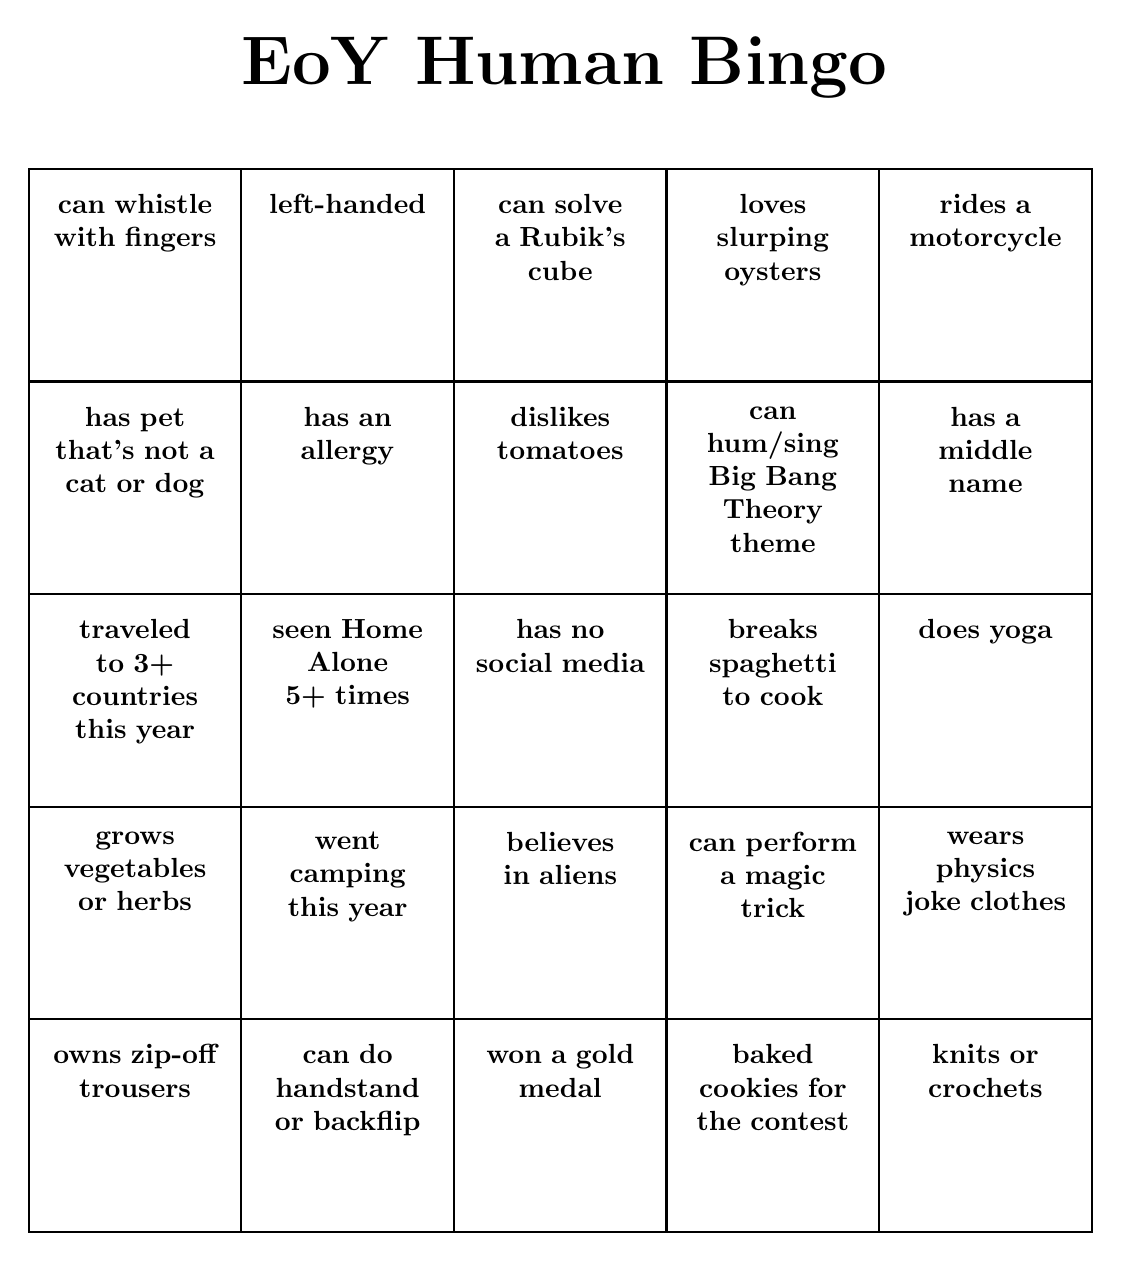
\begin{tikzpicture}
% Set the grid dimensions
\def\cellsize{2.7cm} % Each cell will be 2x2 cm

% Draw the grid and insert the numbers
\draw[thick] (0.0, 0.0) rectangle +(2.7, 2.7);
\node[anchor=north, align=center, text width=2.2cm] at (1.35, 2.5) {\textbf{can whistle with fingers}};
\draw[thick] (2.7, 0.0) rectangle +(2.7, 2.7);
\node[anchor=north, align=center, text width=2.2cm] at (4.050000000000001, 2.5) {\textbf{left-handed}};
\draw[thick] (5.4, 0.0) rectangle +(2.7, 2.7);
\node[anchor=north, align=center, text width=2.2cm] at (6.75, 2.5) {\textbf{can solve a Rubik's cube}};
\draw[thick] (8.100000000000001, 0.0) rectangle +(2.7, 2.7);
\node[anchor=north, align=center, text width=2.2cm] at (9.450000000000001, 2.5) {\textbf{loves slurping oysters}};
\draw[thick] (10.8, 0.0) rectangle +(2.7, 2.7);
\node[anchor=north, align=center, text width=2.2cm] at (12.15, 2.5) {\textbf{rides a motorcycle}};
\draw[thick] (0.0, -2.7) rectangle +(2.7, 2.7);
\node[anchor=north, align=center, text width=2.2cm] at (1.35, -0.2) {\textbf{has pet that's not a cat or dog}};
\draw[thick] (2.7, -2.7) rectangle +(2.7, 2.7);
\node[anchor=north, align=center, text width=2.2cm] at (4.050000000000001, -0.2) {\textbf{has an allergy}};
\draw[thick] (5.4, -2.7) rectangle +(2.7, 2.7);
\node[anchor=north, align=center, text width=2.2cm] at (6.75, -0.2) {\textbf{dislikes tomatoes}};
\draw[thick] (8.100000000000001, -2.7) rectangle +(2.7, 2.7);
\node[anchor=north, align=center, text width=2.2cm] at (9.450000000000001, -0.2) {\textbf{can hum/sing Big Bang Theory theme}};
\draw[thick] (10.8, -2.7) rectangle +(2.7, 2.7);
\node[anchor=north, align=center, text width=2.2cm] at (12.15, -0.2) {\textbf{has a middle name}};
\draw[thick] (0.0, -5.4) rectangle +(2.7, 2.7);
\node[anchor=north, align=center, text width=2.2cm] at (1.35, -2.9000000000000004) {\textbf{traveled to 3+ countries this year}};
\draw[thick] (2.7, -5.4) rectangle +(2.7, 2.7);
\node[anchor=north, align=center, text width=2.2cm] at (4.050000000000001, -2.9000000000000004) {\textbf{seen Home Alone 5+ times}};
\draw[thick] (5.4, -5.4) rectangle +(2.7, 2.7);
\node[anchor=north, align=center, text width=2.2cm] at (6.75, -2.9000000000000004) {\textbf{has no social media}};
\draw[thick] (8.100000000000001, -5.4) rectangle +(2.7, 2.7);
\node[anchor=north, align=center, text width=2.2cm] at (9.450000000000001, -2.9000000000000004) {\textbf{breaks spaghetti to cook}};
\draw[thick] (10.8, -5.4) rectangle +(2.7, 2.7);
\node[anchor=north, align=center, text width=2.2cm] at (12.15, -2.9000000000000004) {\textbf{does yoga}};
\draw[thick] (0.0, -8.100000000000001) rectangle +(2.7, 2.7);
\node[anchor=north, align=center, text width=2.2cm] at (1.35, -5.600000000000001) {\textbf{grows vegetables or herbs}};
\draw[thick] (2.7, -8.100000000000001) rectangle +(2.7, 2.7);
\node[anchor=north, align=center, text width=2.2cm] at (4.050000000000001, -5.600000000000001) {\textbf{went camping this year}};
\draw[thick] (5.4, -8.100000000000001) rectangle +(2.7, 2.7);
\node[anchor=north, align=center, text width=2.2cm] at (6.75, -5.600000000000001) {\textbf{believes in aliens}};
\draw[thick] (8.100000000000001, -8.100000000000001) rectangle +(2.7, 2.7);
\node[anchor=north, align=center, text width=2.2cm] at (9.450000000000001, -5.600000000000001) {\textbf{can perform a magic trick}};
\draw[thick] (10.8, -8.100000000000001) rectangle +(2.7, 2.7);
\node[anchor=north, align=center, text width=2.2cm] at (12.15, -5.600000000000001) {\textbf{wears physics joke clothes}};
\draw[thick] (0.0, -10.8) rectangle +(2.7, 2.7);
\node[anchor=north, align=center, text width=2.2cm] at (1.35, -8.3) {\textbf{owns zip-off trousers}};
\draw[thick] (2.7, -10.8) rectangle +(2.7, 2.7);
\node[anchor=north, align=center, text width=2.2cm] at (4.050000000000001, -8.3) {\textbf{can do handstand or backflip}};
\draw[thick] (5.4, -10.8) rectangle +(2.7, 2.7);
\node[anchor=north, align=center, text width=2.2cm] at (6.75, -8.3) {\textbf{won a gold medal}};
\draw[thick] (8.100000000000001, -10.8) rectangle +(2.7, 2.7);
\node[anchor=north, align=center, text width=2.2cm] at (9.450000000000001, -8.3) {\textbf{baked cookies for the contest}};
\draw[thick] (10.8, -10.8) rectangle +(2.7, 2.7);
\node[anchor=north, align=center, text width=2.2cm] at (12.15, -8.3) {\textbf{knits or crochets}};
\node[anchor=north, font = \Huge] at (6.8, 4.5){\textbf{EoY Human Bingo}};
\end{tikzpicture}
\end{center}
\newpage\begin{center}
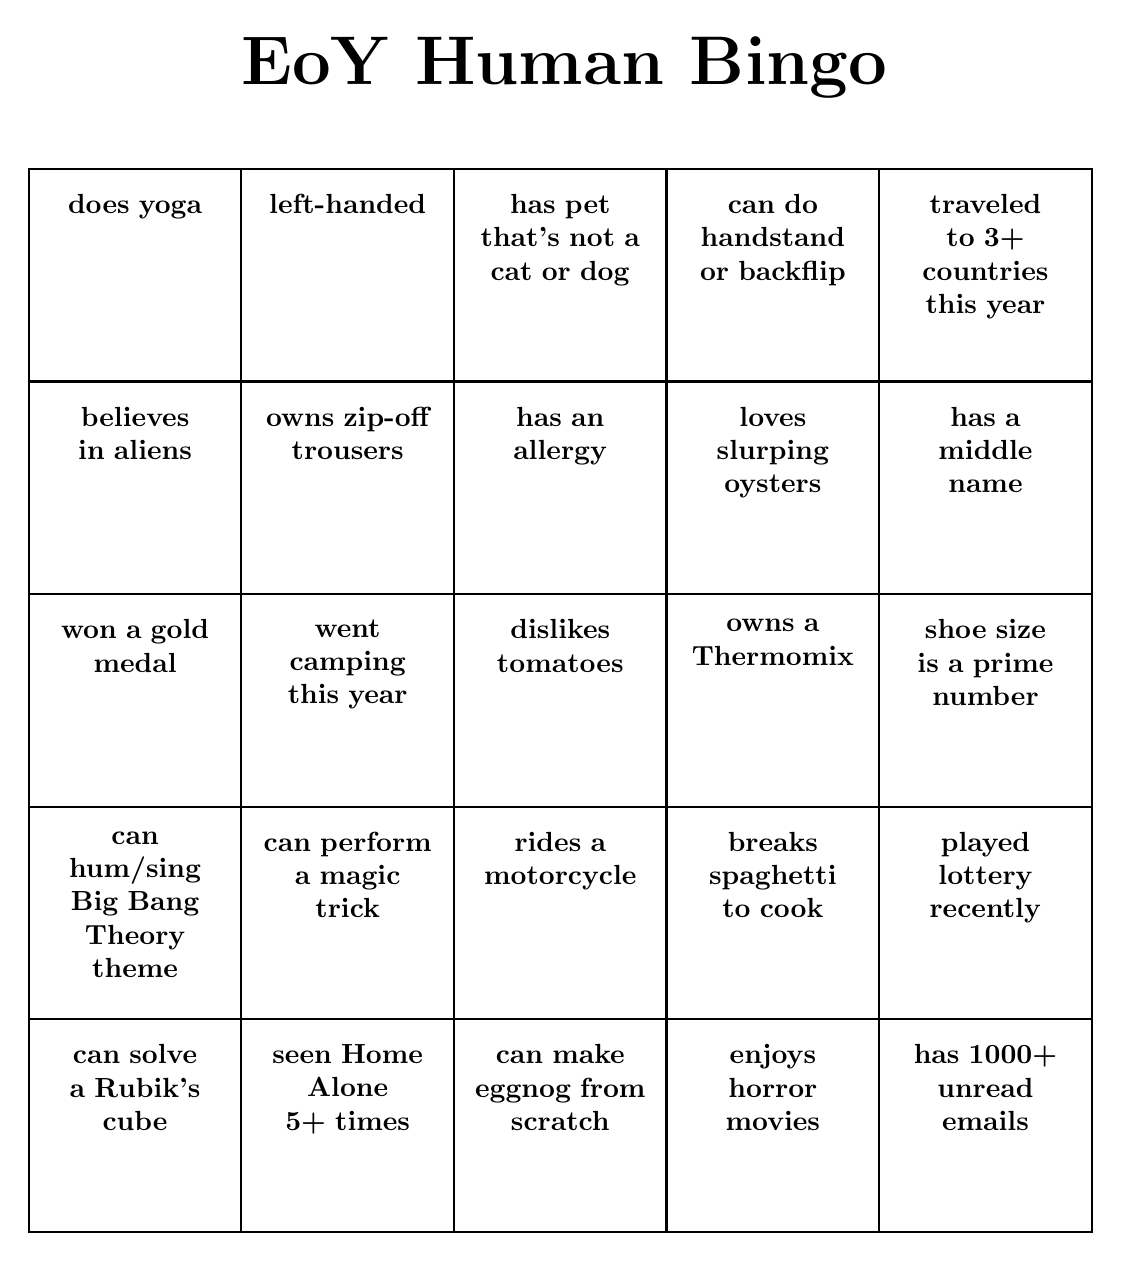
\begin{tikzpicture}
% Set the grid dimensions
\def\cellsize{2.7cm} % Each cell will be 2x2 cm

% Draw the grid and insert the numbers
\draw[thick] (0.0, 0.0) rectangle +(2.7, 2.7);
\node[anchor=north, align=center, text width=2.2cm] at (1.35, 2.5) {\textbf{does yoga}};
\draw[thick] (2.7, 0.0) rectangle +(2.7, 2.7);
\node[anchor=north, align=center, text width=2.2cm] at (4.050000000000001, 2.5) {\textbf{left-handed}};
\draw[thick] (5.4, 0.0) rectangle +(2.7, 2.7);
\node[anchor=north, align=center, text width=2.2cm] at (6.75, 2.5) {\textbf{has pet that's not a cat or dog}};
\draw[thick] (8.100000000000001, 0.0) rectangle +(2.7, 2.7);
\node[anchor=north, align=center, text width=2.2cm] at (9.450000000000001, 2.5) {\textbf{can do handstand or backflip}};
\draw[thick] (10.8, 0.0) rectangle +(2.7, 2.7);
\node[anchor=north, align=center, text width=2.2cm] at (12.15, 2.5) {\textbf{traveled to 3+ countries this year}};
\draw[thick] (0.0, -2.7) rectangle +(2.7, 2.7);
\node[anchor=north, align=center, text width=2.2cm] at (1.35, -0.2) {\textbf{believes in aliens}};
\draw[thick] (2.7, -2.7) rectangle +(2.7, 2.7);
\node[anchor=north, align=center, text width=2.2cm] at (4.050000000000001, -0.2) {\textbf{owns zip-off trousers}};
\draw[thick] (5.4, -2.7) rectangle +(2.7, 2.7);
\node[anchor=north, align=center, text width=2.2cm] at (6.75, -0.2) {\textbf{has an allergy}};
\draw[thick] (8.100000000000001, -2.7) rectangle +(2.7, 2.7);
\node[anchor=north, align=center, text width=2.2cm] at (9.450000000000001, -0.2) {\textbf{loves slurping oysters}};
\draw[thick] (10.8, -2.7) rectangle +(2.7, 2.7);
\node[anchor=north, align=center, text width=2.2cm] at (12.15, -0.2) {\textbf{has a middle name}};
\draw[thick] (0.0, -5.4) rectangle +(2.7, 2.7);
\node[anchor=north, align=center, text width=2.2cm] at (1.35, -2.9000000000000004) {\textbf{won a gold medal}};
\draw[thick] (2.7, -5.4) rectangle +(2.7, 2.7);
\node[anchor=north, align=center, text width=2.2cm] at (4.050000000000001, -2.9000000000000004) {\textbf{went camping this year}};
\draw[thick] (5.4, -5.4) rectangle +(2.7, 2.7);
\node[anchor=north, align=center, text width=2.2cm] at (6.75, -2.9000000000000004) {\textbf{dislikes tomatoes}};
\draw[thick] (8.100000000000001, -5.4) rectangle +(2.7, 2.7);
\node[anchor=north, align=center, text width=2.2cm] at (9.450000000000001, -2.9000000000000004) {\textbf{owns a Thermomix}};
\draw[thick] (10.8, -5.4) rectangle +(2.7, 2.7);
\node[anchor=north, align=center, text width=2.2cm] at (12.15, -2.9000000000000004) {\textbf{shoe size is a prime number}};
\draw[thick] (0.0, -8.100000000000001) rectangle +(2.7, 2.7);
\node[anchor=north, align=center, text width=2.2cm] at (1.35, -5.600000000000001) {\textbf{can hum/sing Big Bang Theory theme}};
\draw[thick] (2.7, -8.100000000000001) rectangle +(2.7, 2.7);
\node[anchor=north, align=center, text width=2.2cm] at (4.050000000000001, -5.600000000000001) {\textbf{can perform a magic trick}};
\draw[thick] (5.4, -8.100000000000001) rectangle +(2.7, 2.7);
\node[anchor=north, align=center, text width=2.2cm] at (6.75, -5.600000000000001) {\textbf{rides a motorcycle}};
\draw[thick] (8.100000000000001, -8.100000000000001) rectangle +(2.7, 2.7);
\node[anchor=north, align=center, text width=2.2cm] at (9.450000000000001, -5.600000000000001) {\textbf{breaks spaghetti to cook}};
\draw[thick] (10.8, -8.100000000000001) rectangle +(2.7, 2.7);
\node[anchor=north, align=center, text width=2.2cm] at (12.15, -5.600000000000001) {\textbf{played lottery recently}};
\draw[thick] (0.0, -10.8) rectangle +(2.7, 2.7);
\node[anchor=north, align=center, text width=2.2cm] at (1.35, -8.3) {\textbf{can solve a Rubik's cube}};
\draw[thick] (2.7, -10.8) rectangle +(2.7, 2.7);
\node[anchor=north, align=center, text width=2.2cm] at (4.050000000000001, -8.3) {\textbf{seen Home Alone 5+ times}};
\draw[thick] (5.4, -10.8) rectangle +(2.7, 2.7);
\node[anchor=north, align=center, text width=2.2cm] at (6.75, -8.3) {\textbf{can make eggnog from scratch}};
\draw[thick] (8.100000000000001, -10.8) rectangle +(2.7, 2.7);
\node[anchor=north, align=center, text width=2.2cm] at (9.450000000000001, -8.3) {\textbf{enjoys horror movies}};
\draw[thick] (10.8, -10.8) rectangle +(2.7, 2.7);
\node[anchor=north, align=center, text width=2.2cm] at (12.15, -8.3) {\textbf{has 1000+ unread emails}};
\node[anchor=north, font = \Huge] at (6.8, 4.5){\textbf{EoY Human Bingo}};
\end{tikzpicture}
\end{center}
\newpage\begin{center}
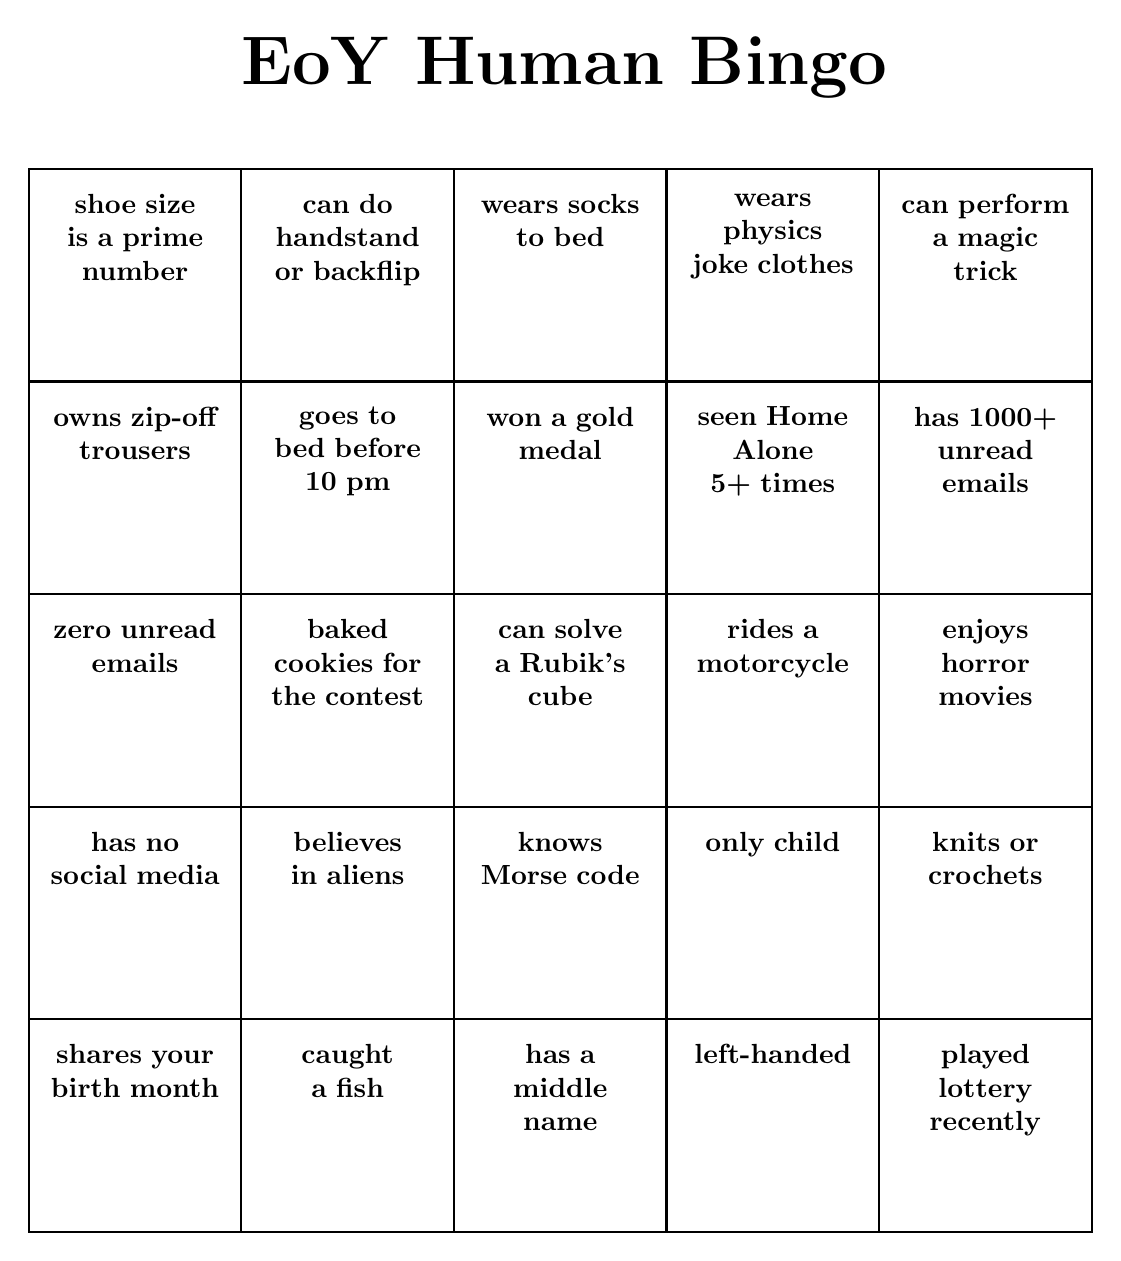
\begin{tikzpicture}
% Set the grid dimensions
\def\cellsize{2.7cm} % Each cell will be 2x2 cm

% Draw the grid and insert the numbers
\draw[thick] (0.0, 0.0) rectangle +(2.7, 2.7);
\node[anchor=north, align=center, text width=2.2cm] at (1.35, 2.5) {\textbf{shoe size is a prime number}};
\draw[thick] (2.7, 0.0) rectangle +(2.7, 2.7);
\node[anchor=north, align=center, text width=2.2cm] at (4.050000000000001, 2.5) {\textbf{can do handstand or backflip}};
\draw[thick] (5.4, 0.0) rectangle +(2.7, 2.7);
\node[anchor=north, align=center, text width=2.2cm] at (6.75, 2.5) {\textbf{wears socks to bed}};
\draw[thick] (8.100000000000001, 0.0) rectangle +(2.7, 2.7);
\node[anchor=north, align=center, text width=2.2cm] at (9.450000000000001, 2.5) {\textbf{wears physics joke clothes}};
\draw[thick] (10.8, 0.0) rectangle +(2.7, 2.7);
\node[anchor=north, align=center, text width=2.2cm] at (12.15, 2.5) {\textbf{can perform a magic trick}};
\draw[thick] (0.0, -2.7) rectangle +(2.7, 2.7);
\node[anchor=north, align=center, text width=2.2cm] at (1.35, -0.2) {\textbf{owns zip-off trousers}};
\draw[thick] (2.7, -2.7) rectangle +(2.7, 2.7);
\node[anchor=north, align=center, text width=2.2cm] at (4.050000000000001, -0.2) {\textbf{goes to bed before 10 pm}};
\draw[thick] (5.4, -2.7) rectangle +(2.7, 2.7);
\node[anchor=north, align=center, text width=2.2cm] at (6.75, -0.2) {\textbf{won a gold medal}};
\draw[thick] (8.100000000000001, -2.7) rectangle +(2.7, 2.7);
\node[anchor=north, align=center, text width=2.2cm] at (9.450000000000001, -0.2) {\textbf{seen Home Alone 5+ times}};
\draw[thick] (10.8, -2.7) rectangle +(2.7, 2.7);
\node[anchor=north, align=center, text width=2.2cm] at (12.15, -0.2) {\textbf{has 1000+ unread emails}};
\draw[thick] (0.0, -5.4) rectangle +(2.7, 2.7);
\node[anchor=north, align=center, text width=2.2cm] at (1.35, -2.9000000000000004) {\textbf{zero unread emails}};
\draw[thick] (2.7, -5.4) rectangle +(2.7, 2.7);
\node[anchor=north, align=center, text width=2.2cm] at (4.050000000000001, -2.9000000000000004) {\textbf{baked cookies for the contest}};
\draw[thick] (5.4, -5.4) rectangle +(2.7, 2.7);
\node[anchor=north, align=center, text width=2.2cm] at (6.75, -2.9000000000000004) {\textbf{can solve a Rubik's cube}};
\draw[thick] (8.100000000000001, -5.4) rectangle +(2.7, 2.7);
\node[anchor=north, align=center, text width=2.2cm] at (9.450000000000001, -2.9000000000000004) {\textbf{rides a motorcycle}};
\draw[thick] (10.8, -5.4) rectangle +(2.7, 2.7);
\node[anchor=north, align=center, text width=2.2cm] at (12.15, -2.9000000000000004) {\textbf{enjoys horror movies}};
\draw[thick] (0.0, -8.100000000000001) rectangle +(2.7, 2.7);
\node[anchor=north, align=center, text width=2.2cm] at (1.35, -5.600000000000001) {\textbf{has no social media}};
\draw[thick] (2.7, -8.100000000000001) rectangle +(2.7, 2.7);
\node[anchor=north, align=center, text width=2.2cm] at (4.050000000000001, -5.600000000000001) {\textbf{believes in aliens}};
\draw[thick] (5.4, -8.100000000000001) rectangle +(2.7, 2.7);
\node[anchor=north, align=center, text width=2.2cm] at (6.75, -5.600000000000001) {\textbf{knows Morse code}};
\draw[thick] (8.100000000000001, -8.100000000000001) rectangle +(2.7, 2.7);
\node[anchor=north, align=center, text width=2.2cm] at (9.450000000000001, -5.600000000000001) {\textbf{only child}};
\draw[thick] (10.8, -8.100000000000001) rectangle +(2.7, 2.7);
\node[anchor=north, align=center, text width=2.2cm] at (12.15, -5.600000000000001) {\textbf{knits or crochets}};
\draw[thick] (0.0, -10.8) rectangle +(2.7, 2.7);
\node[anchor=north, align=center, text width=2.2cm] at (1.35, -8.3) {\textbf{shares your birth month}};
\draw[thick] (2.7, -10.8) rectangle +(2.7, 2.7);
\node[anchor=north, align=center, text width=2.2cm] at (4.050000000000001, -8.3) {\textbf{caught a fish}};
\draw[thick] (5.4, -10.8) rectangle +(2.7, 2.7);
\node[anchor=north, align=center, text width=2.2cm] at (6.75, -8.3) {\textbf{has a middle name}};
\draw[thick] (8.100000000000001, -10.8) rectangle +(2.7, 2.7);
\node[anchor=north, align=center, text width=2.2cm] at (9.450000000000001, -8.3) {\textbf{left-handed}};
\draw[thick] (10.8, -10.8) rectangle +(2.7, 2.7);
\node[anchor=north, align=center, text width=2.2cm] at (12.15, -8.3) {\textbf{played lottery recently}};
\node[anchor=north, font = \Huge] at (6.8, 4.5){\textbf{EoY Human Bingo}};
\end{tikzpicture}
\end{center}
\newpage\begin{center}
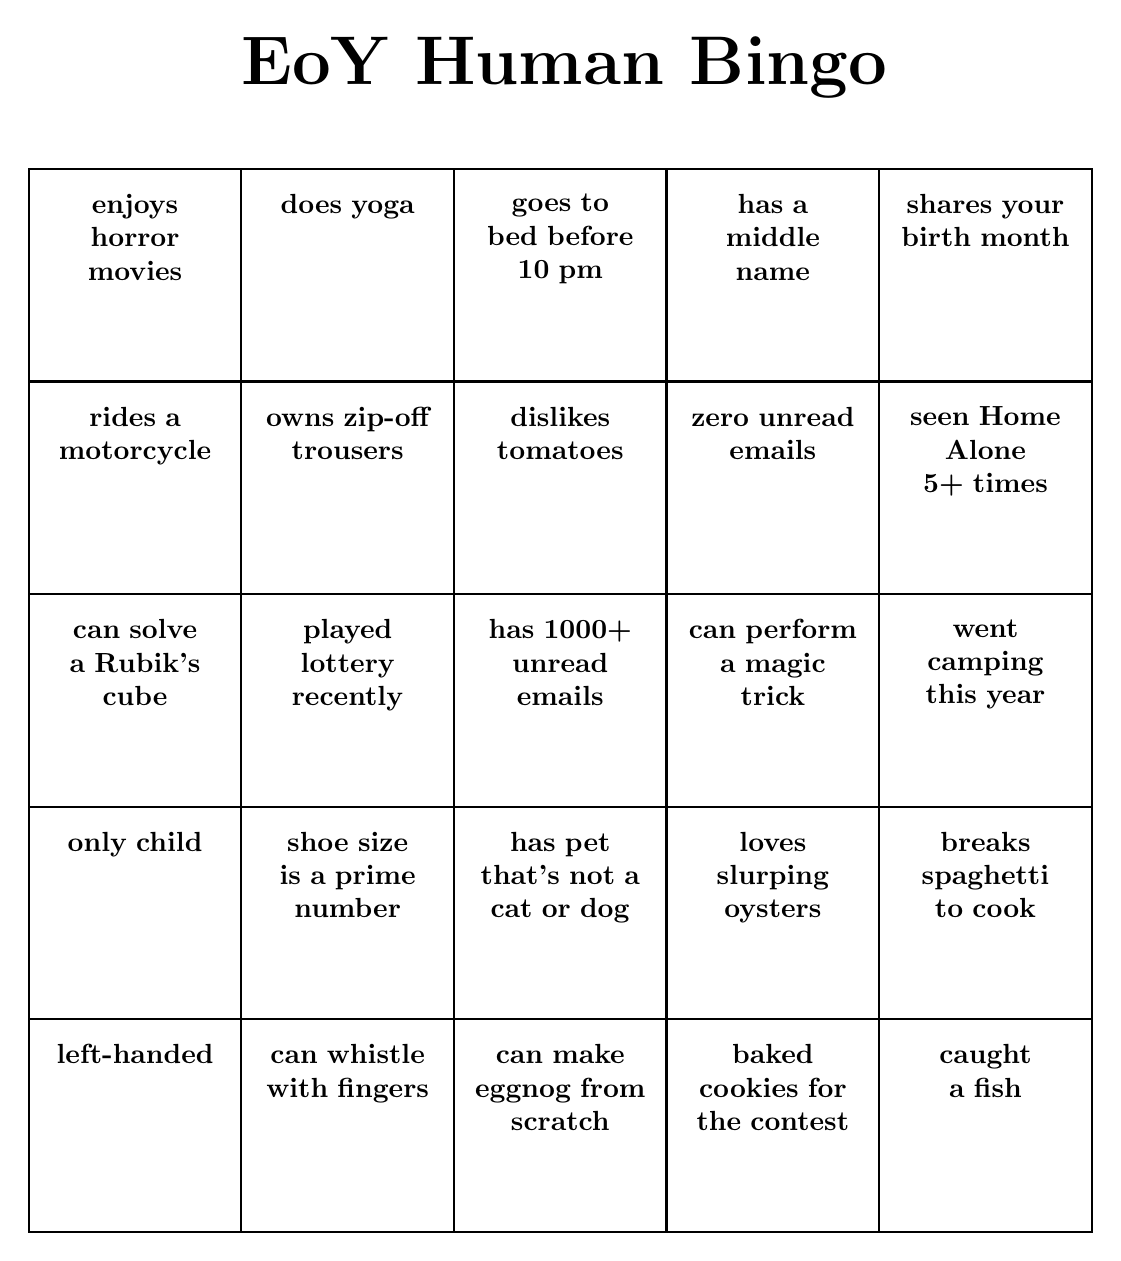
\begin{tikzpicture}
% Set the grid dimensions
\def\cellsize{2.7cm} % Each cell will be 2x2 cm

% Draw the grid and insert the numbers
\draw[thick] (0.0, 0.0) rectangle +(2.7, 2.7);
\node[anchor=north, align=center, text width=2.2cm] at (1.35, 2.5) {\textbf{enjoys horror movies}};
\draw[thick] (2.7, 0.0) rectangle +(2.7, 2.7);
\node[anchor=north, align=center, text width=2.2cm] at (4.050000000000001, 2.5) {\textbf{does yoga}};
\draw[thick] (5.4, 0.0) rectangle +(2.7, 2.7);
\node[anchor=north, align=center, text width=2.2cm] at (6.75, 2.5) {\textbf{goes to bed before 10 pm}};
\draw[thick] (8.100000000000001, 0.0) rectangle +(2.7, 2.7);
\node[anchor=north, align=center, text width=2.2cm] at (9.450000000000001, 2.5) {\textbf{has a middle name}};
\draw[thick] (10.8, 0.0) rectangle +(2.7, 2.7);
\node[anchor=north, align=center, text width=2.2cm] at (12.15, 2.5) {\textbf{shares your birth month}};
\draw[thick] (0.0, -2.7) rectangle +(2.7, 2.7);
\node[anchor=north, align=center, text width=2.2cm] at (1.35, -0.2) {\textbf{rides a motorcycle}};
\draw[thick] (2.7, -2.7) rectangle +(2.7, 2.7);
\node[anchor=north, align=center, text width=2.2cm] at (4.050000000000001, -0.2) {\textbf{owns zip-off trousers}};
\draw[thick] (5.4, -2.7) rectangle +(2.7, 2.7);
\node[anchor=north, align=center, text width=2.2cm] at (6.75, -0.2) {\textbf{dislikes tomatoes}};
\draw[thick] (8.100000000000001, -2.7) rectangle +(2.7, 2.7);
\node[anchor=north, align=center, text width=2.2cm] at (9.450000000000001, -0.2) {\textbf{zero unread emails}};
\draw[thick] (10.8, -2.7) rectangle +(2.7, 2.7);
\node[anchor=north, align=center, text width=2.2cm] at (12.15, -0.2) {\textbf{seen Home Alone 5+ times}};
\draw[thick] (0.0, -5.4) rectangle +(2.7, 2.7);
\node[anchor=north, align=center, text width=2.2cm] at (1.35, -2.9000000000000004) {\textbf{can solve a Rubik's cube}};
\draw[thick] (2.7, -5.4) rectangle +(2.7, 2.7);
\node[anchor=north, align=center, text width=2.2cm] at (4.050000000000001, -2.9000000000000004) {\textbf{played lottery recently}};
\draw[thick] (5.4, -5.4) rectangle +(2.7, 2.7);
\node[anchor=north, align=center, text width=2.2cm] at (6.75, -2.9000000000000004) {\textbf{has 1000+ unread emails}};
\draw[thick] (8.100000000000001, -5.4) rectangle +(2.7, 2.7);
\node[anchor=north, align=center, text width=2.2cm] at (9.450000000000001, -2.9000000000000004) {\textbf{can perform a magic trick}};
\draw[thick] (10.8, -5.4) rectangle +(2.7, 2.7);
\node[anchor=north, align=center, text width=2.2cm] at (12.15, -2.9000000000000004) {\textbf{went camping this year}};
\draw[thick] (0.0, -8.100000000000001) rectangle +(2.7, 2.7);
\node[anchor=north, align=center, text width=2.2cm] at (1.35, -5.600000000000001) {\textbf{only child}};
\draw[thick] (2.7, -8.100000000000001) rectangle +(2.7, 2.7);
\node[anchor=north, align=center, text width=2.2cm] at (4.050000000000001, -5.600000000000001) {\textbf{shoe size is a prime number}};
\draw[thick] (5.4, -8.100000000000001) rectangle +(2.7, 2.7);
\node[anchor=north, align=center, text width=2.2cm] at (6.75, -5.600000000000001) {\textbf{has pet that's not a cat or dog}};
\draw[thick] (8.100000000000001, -8.100000000000001) rectangle +(2.7, 2.7);
\node[anchor=north, align=center, text width=2.2cm] at (9.450000000000001, -5.600000000000001) {\textbf{loves slurping oysters}};
\draw[thick] (10.8, -8.100000000000001) rectangle +(2.7, 2.7);
\node[anchor=north, align=center, text width=2.2cm] at (12.15, -5.600000000000001) {\textbf{breaks spaghetti to cook}};
\draw[thick] (0.0, -10.8) rectangle +(2.7, 2.7);
\node[anchor=north, align=center, text width=2.2cm] at (1.35, -8.3) {\textbf{left-handed}};
\draw[thick] (2.7, -10.8) rectangle +(2.7, 2.7);
\node[anchor=north, align=center, text width=2.2cm] at (4.050000000000001, -8.3) {\textbf{can whistle with fingers}};
\draw[thick] (5.4, -10.8) rectangle +(2.7, 2.7);
\node[anchor=north, align=center, text width=2.2cm] at (6.75, -8.3) {\textbf{can make eggnog from scratch}};
\draw[thick] (8.100000000000001, -10.8) rectangle +(2.7, 2.7);
\node[anchor=north, align=center, text width=2.2cm] at (9.450000000000001, -8.3) {\textbf{baked cookies for the contest}};
\draw[thick] (10.8, -10.8) rectangle +(2.7, 2.7);
\node[anchor=north, align=center, text width=2.2cm] at (12.15, -8.3) {\textbf{caught a fish}};
\node[anchor=north, font = \Huge] at (6.8, 4.5){\textbf{EoY Human Bingo}};
\end{tikzpicture}
\end{center}
\newpage\begin{center}
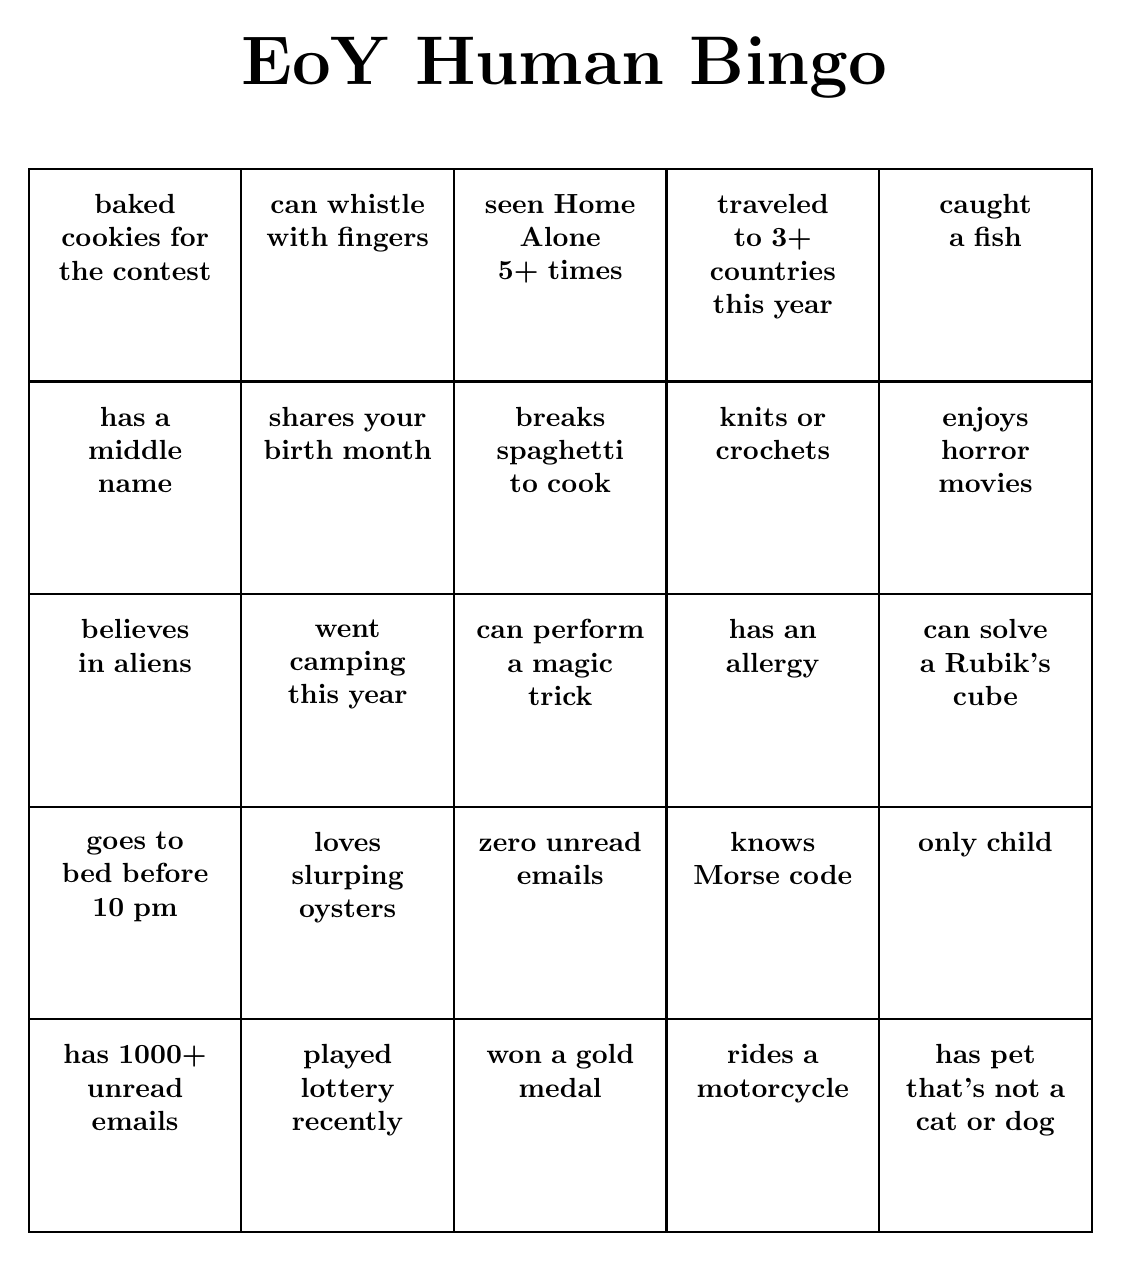
\begin{tikzpicture}
% Set the grid dimensions
\def\cellsize{2.7cm} % Each cell will be 2x2 cm

% Draw the grid and insert the numbers
\draw[thick] (0.0, 0.0) rectangle +(2.7, 2.7);
\node[anchor=north, align=center, text width=2.2cm] at (1.35, 2.5) {\textbf{baked cookies for the contest}};
\draw[thick] (2.7, 0.0) rectangle +(2.7, 2.7);
\node[anchor=north, align=center, text width=2.2cm] at (4.050000000000001, 2.5) {\textbf{can whistle with fingers}};
\draw[thick] (5.4, 0.0) rectangle +(2.7, 2.7);
\node[anchor=north, align=center, text width=2.2cm] at (6.75, 2.5) {\textbf{seen Home Alone 5+ times}};
\draw[thick] (8.100000000000001, 0.0) rectangle +(2.7, 2.7);
\node[anchor=north, align=center, text width=2.2cm] at (9.450000000000001, 2.5) {\textbf{traveled to 3+ countries this year}};
\draw[thick] (10.8, 0.0) rectangle +(2.7, 2.7);
\node[anchor=north, align=center, text width=2.2cm] at (12.15, 2.5) {\textbf{caught a fish}};
\draw[thick] (0.0, -2.7) rectangle +(2.7, 2.7);
\node[anchor=north, align=center, text width=2.2cm] at (1.35, -0.2) {\textbf{has a middle name}};
\draw[thick] (2.7, -2.7) rectangle +(2.7, 2.7);
\node[anchor=north, align=center, text width=2.2cm] at (4.050000000000001, -0.2) {\textbf{shares your birth month}};
\draw[thick] (5.4, -2.7) rectangle +(2.7, 2.7);
\node[anchor=north, align=center, text width=2.2cm] at (6.75, -0.2) {\textbf{breaks spaghetti to cook}};
\draw[thick] (8.100000000000001, -2.7) rectangle +(2.7, 2.7);
\node[anchor=north, align=center, text width=2.2cm] at (9.450000000000001, -0.2) {\textbf{knits or crochets}};
\draw[thick] (10.8, -2.7) rectangle +(2.7, 2.7);
\node[anchor=north, align=center, text width=2.2cm] at (12.15, -0.2) {\textbf{enjoys horror movies}};
\draw[thick] (0.0, -5.4) rectangle +(2.7, 2.7);
\node[anchor=north, align=center, text width=2.2cm] at (1.35, -2.9000000000000004) {\textbf{believes in aliens}};
\draw[thick] (2.7, -5.4) rectangle +(2.7, 2.7);
\node[anchor=north, align=center, text width=2.2cm] at (4.050000000000001, -2.9000000000000004) {\textbf{went camping this year}};
\draw[thick] (5.4, -5.4) rectangle +(2.7, 2.7);
\node[anchor=north, align=center, text width=2.2cm] at (6.75, -2.9000000000000004) {\textbf{can perform a magic trick}};
\draw[thick] (8.100000000000001, -5.4) rectangle +(2.7, 2.7);
\node[anchor=north, align=center, text width=2.2cm] at (9.450000000000001, -2.9000000000000004) {\textbf{has an allergy}};
\draw[thick] (10.8, -5.4) rectangle +(2.7, 2.7);
\node[anchor=north, align=center, text width=2.2cm] at (12.15, -2.9000000000000004) {\textbf{can solve a Rubik's cube}};
\draw[thick] (0.0, -8.100000000000001) rectangle +(2.7, 2.7);
\node[anchor=north, align=center, text width=2.2cm] at (1.35, -5.600000000000001) {\textbf{goes to bed before 10 pm}};
\draw[thick] (2.7, -8.100000000000001) rectangle +(2.7, 2.7);
\node[anchor=north, align=center, text width=2.2cm] at (4.050000000000001, -5.600000000000001) {\textbf{loves slurping oysters}};
\draw[thick] (5.4, -8.100000000000001) rectangle +(2.7, 2.7);
\node[anchor=north, align=center, text width=2.2cm] at (6.75, -5.600000000000001) {\textbf{zero unread emails}};
\draw[thick] (8.100000000000001, -8.100000000000001) rectangle +(2.7, 2.7);
\node[anchor=north, align=center, text width=2.2cm] at (9.450000000000001, -5.600000000000001) {\textbf{knows Morse code}};
\draw[thick] (10.8, -8.100000000000001) rectangle +(2.7, 2.7);
\node[anchor=north, align=center, text width=2.2cm] at (12.15, -5.600000000000001) {\textbf{only child}};
\draw[thick] (0.0, -10.8) rectangle +(2.7, 2.7);
\node[anchor=north, align=center, text width=2.2cm] at (1.35, -8.3) {\textbf{has 1000+ unread emails}};
\draw[thick] (2.7, -10.8) rectangle +(2.7, 2.7);
\node[anchor=north, align=center, text width=2.2cm] at (4.050000000000001, -8.3) {\textbf{played lottery recently}};
\draw[thick] (5.4, -10.8) rectangle +(2.7, 2.7);
\node[anchor=north, align=center, text width=2.2cm] at (6.75, -8.3) {\textbf{won a gold medal}};
\draw[thick] (8.100000000000001, -10.8) rectangle +(2.7, 2.7);
\node[anchor=north, align=center, text width=2.2cm] at (9.450000000000001, -8.3) {\textbf{rides a motorcycle}};
\draw[thick] (10.8, -10.8) rectangle +(2.7, 2.7);
\node[anchor=north, align=center, text width=2.2cm] at (12.15, -8.3) {\textbf{has pet that's not a cat or dog}};
\node[anchor=north, font = \Huge] at (6.8, 4.5){\textbf{EoY Human Bingo}};
\end{tikzpicture}
\end{center}
\newpage\begin{center}
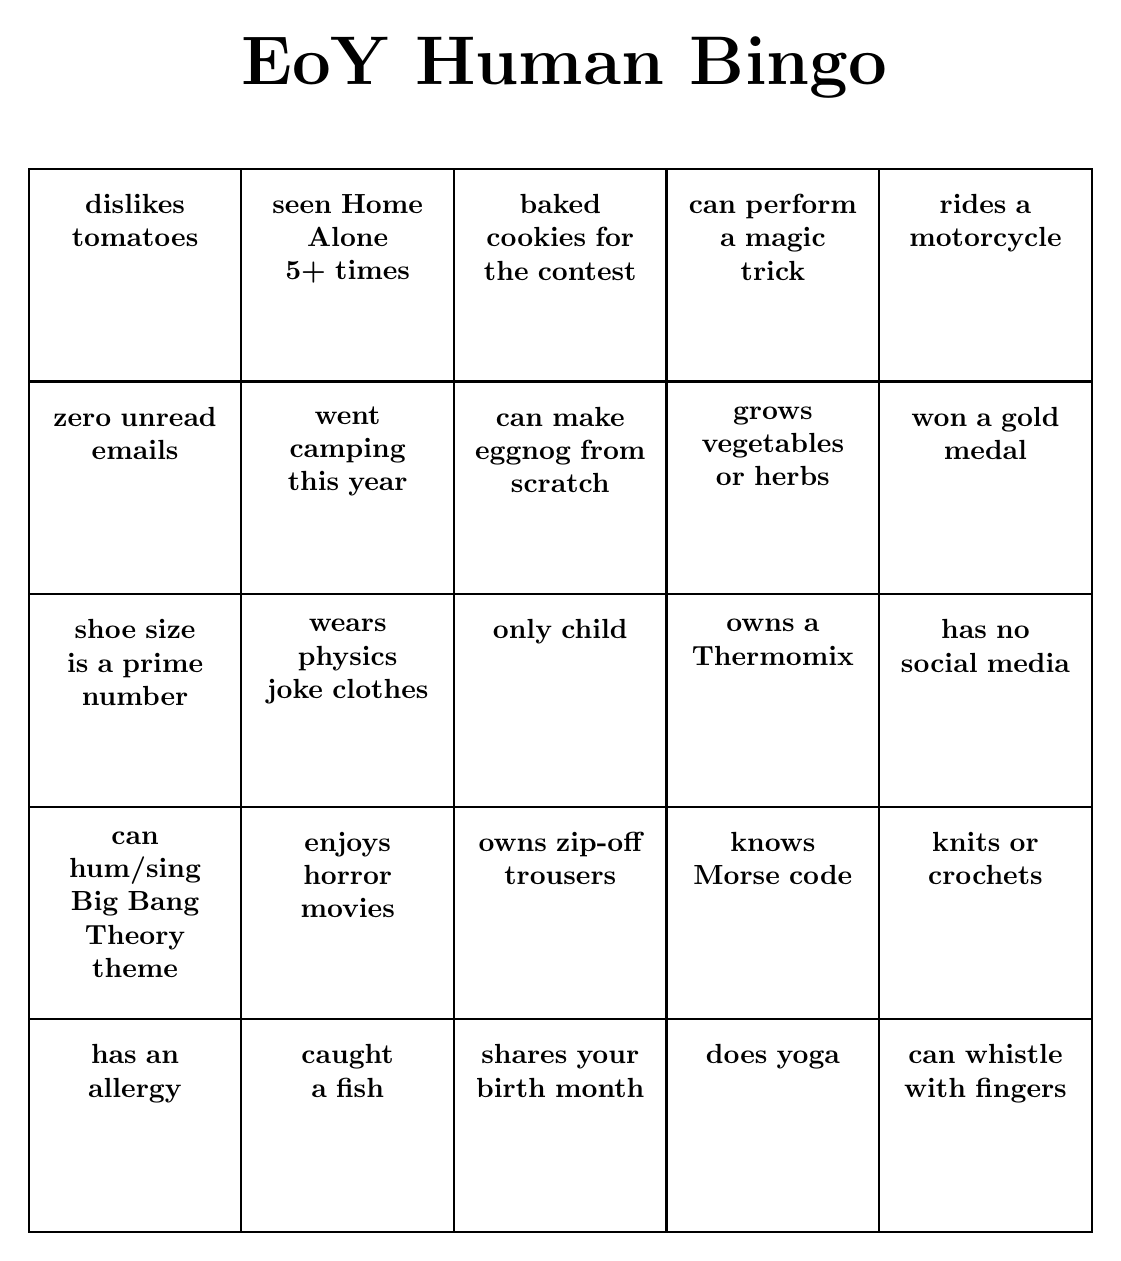
\begin{tikzpicture}
% Set the grid dimensions
\def\cellsize{2.7cm} % Each cell will be 2x2 cm

% Draw the grid and insert the numbers
\draw[thick] (0.0, 0.0) rectangle +(2.7, 2.7);
\node[anchor=north, align=center, text width=2.2cm] at (1.35, 2.5) {\textbf{dislikes tomatoes}};
\draw[thick] (2.7, 0.0) rectangle +(2.7, 2.7);
\node[anchor=north, align=center, text width=2.2cm] at (4.050000000000001, 2.5) {\textbf{seen Home Alone 5+ times}};
\draw[thick] (5.4, 0.0) rectangle +(2.7, 2.7);
\node[anchor=north, align=center, text width=2.2cm] at (6.75, 2.5) {\textbf{baked cookies for the contest}};
\draw[thick] (8.100000000000001, 0.0) rectangle +(2.7, 2.7);
\node[anchor=north, align=center, text width=2.2cm] at (9.450000000000001, 2.5) {\textbf{can perform a magic trick}};
\draw[thick] (10.8, 0.0) rectangle +(2.7, 2.7);
\node[anchor=north, align=center, text width=2.2cm] at (12.15, 2.5) {\textbf{rides a motorcycle}};
\draw[thick] (0.0, -2.7) rectangle +(2.7, 2.7);
\node[anchor=north, align=center, text width=2.2cm] at (1.35, -0.2) {\textbf{zero unread emails}};
\draw[thick] (2.7, -2.7) rectangle +(2.7, 2.7);
\node[anchor=north, align=center, text width=2.2cm] at (4.050000000000001, -0.2) {\textbf{went camping this year}};
\draw[thick] (5.4, -2.7) rectangle +(2.7, 2.7);
\node[anchor=north, align=center, text width=2.2cm] at (6.75, -0.2) {\textbf{can make eggnog from scratch}};
\draw[thick] (8.100000000000001, -2.7) rectangle +(2.7, 2.7);
\node[anchor=north, align=center, text width=2.2cm] at (9.450000000000001, -0.2) {\textbf{grows vegetables or herbs}};
\draw[thick] (10.8, -2.7) rectangle +(2.7, 2.7);
\node[anchor=north, align=center, text width=2.2cm] at (12.15, -0.2) {\textbf{won a gold medal}};
\draw[thick] (0.0, -5.4) rectangle +(2.7, 2.7);
\node[anchor=north, align=center, text width=2.2cm] at (1.35, -2.9000000000000004) {\textbf{shoe size is a prime number}};
\draw[thick] (2.7, -5.4) rectangle +(2.7, 2.7);
\node[anchor=north, align=center, text width=2.2cm] at (4.050000000000001, -2.9000000000000004) {\textbf{wears physics joke clothes}};
\draw[thick] (5.4, -5.4) rectangle +(2.7, 2.7);
\node[anchor=north, align=center, text width=2.2cm] at (6.75, -2.9000000000000004) {\textbf{only child}};
\draw[thick] (8.100000000000001, -5.4) rectangle +(2.7, 2.7);
\node[anchor=north, align=center, text width=2.2cm] at (9.450000000000001, -2.9000000000000004) {\textbf{owns a Thermomix}};
\draw[thick] (10.8, -5.4) rectangle +(2.7, 2.7);
\node[anchor=north, align=center, text width=2.2cm] at (12.15, -2.9000000000000004) {\textbf{has no social media}};
\draw[thick] (0.0, -8.100000000000001) rectangle +(2.7, 2.7);
\node[anchor=north, align=center, text width=2.2cm] at (1.35, -5.600000000000001) {\textbf{can hum/sing Big Bang Theory theme}};
\draw[thick] (2.7, -8.100000000000001) rectangle +(2.7, 2.7);
\node[anchor=north, align=center, text width=2.2cm] at (4.050000000000001, -5.600000000000001) {\textbf{enjoys horror movies}};
\draw[thick] (5.4, -8.100000000000001) rectangle +(2.7, 2.7);
\node[anchor=north, align=center, text width=2.2cm] at (6.75, -5.600000000000001) {\textbf{owns zip-off trousers}};
\draw[thick] (8.100000000000001, -8.100000000000001) rectangle +(2.7, 2.7);
\node[anchor=north, align=center, text width=2.2cm] at (9.450000000000001, -5.600000000000001) {\textbf{knows Morse code}};
\draw[thick] (10.8, -8.100000000000001) rectangle +(2.7, 2.7);
\node[anchor=north, align=center, text width=2.2cm] at (12.15, -5.600000000000001) {\textbf{knits or crochets}};
\draw[thick] (0.0, -10.8) rectangle +(2.7, 2.7);
\node[anchor=north, align=center, text width=2.2cm] at (1.35, -8.3) {\textbf{has an allergy}};
\draw[thick] (2.7, -10.8) rectangle +(2.7, 2.7);
\node[anchor=north, align=center, text width=2.2cm] at (4.050000000000001, -8.3) {\textbf{caught a fish}};
\draw[thick] (5.4, -10.8) rectangle +(2.7, 2.7);
\node[anchor=north, align=center, text width=2.2cm] at (6.75, -8.3) {\textbf{shares your birth month}};
\draw[thick] (8.100000000000001, -10.8) rectangle +(2.7, 2.7);
\node[anchor=north, align=center, text width=2.2cm] at (9.450000000000001, -8.3) {\textbf{does yoga}};
\draw[thick] (10.8, -10.8) rectangle +(2.7, 2.7);
\node[anchor=north, align=center, text width=2.2cm] at (12.15, -8.3) {\textbf{can whistle with fingers}};
\node[anchor=north, font = \Huge] at (6.8, 4.5){\textbf{EoY Human Bingo}};
\end{tikzpicture}
\end{center}
